% Options for packages loaded elsewhere
\PassOptionsToPackage{unicode}{hyperref}
\PassOptionsToPackage{hyphens}{url}
%
\documentclass[
  letterpaper,
]{scrbook}

\usepackage{amsmath,amssymb}
\usepackage{lmodern}
\usepackage{iftex}
\ifPDFTeX
  \usepackage[T1]{fontenc}
  \usepackage[utf8]{inputenc}
  \usepackage{textcomp} % provide euro and other symbols
\else % if luatex or xetex
  \usepackage{unicode-math}
  \defaultfontfeatures{Scale=MatchLowercase}
  \defaultfontfeatures[\rmfamily]{Ligatures=TeX,Scale=1}
\fi
% Use upquote if available, for straight quotes in verbatim environments
\IfFileExists{upquote.sty}{\usepackage{upquote}}{}
\IfFileExists{microtype.sty}{% use microtype if available
  \usepackage[]{microtype}
  \UseMicrotypeSet[protrusion]{basicmath} % disable protrusion for tt fonts
}{}
\makeatletter
\@ifundefined{KOMAClassName}{% if non-KOMA class
  \IfFileExists{parskip.sty}{%
    \usepackage{parskip}
  }{% else
    \setlength{\parindent}{0pt}
    \setlength{\parskip}{6pt plus 2pt minus 1pt}}
}{% if KOMA class
  \KOMAoptions{parskip=half}}
\makeatother
\usepackage{xcolor}
\setlength{\emergencystretch}{3em} % prevent overfull lines
\setcounter{secnumdepth}{5}
% Make \paragraph and \subparagraph free-standing
\ifx\paragraph\undefined\else
  \let\oldparagraph\paragraph
  \renewcommand{\paragraph}[1]{\oldparagraph{#1}\mbox{}}
\fi
\ifx\subparagraph\undefined\else
  \let\oldsubparagraph\subparagraph
  \renewcommand{\subparagraph}[1]{\oldsubparagraph{#1}\mbox{}}
\fi


\providecommand{\tightlist}{%
  \setlength{\itemsep}{0pt}\setlength{\parskip}{0pt}}\usepackage{longtable,booktabs,array}
\usepackage{calc} % for calculating minipage widths
% Correct order of tables after \paragraph or \subparagraph
\usepackage{etoolbox}
\makeatletter
\patchcmd\longtable{\par}{\if@noskipsec\mbox{}\fi\par}{}{}
\makeatother
% Allow footnotes in longtable head/foot
\IfFileExists{footnotehyper.sty}{\usepackage{footnotehyper}}{\usepackage{footnote}}
\makesavenoteenv{longtable}
\usepackage{graphicx}
\makeatletter
\def\maxwidth{\ifdim\Gin@nat@width>\linewidth\linewidth\else\Gin@nat@width\fi}
\def\maxheight{\ifdim\Gin@nat@height>\textheight\textheight\else\Gin@nat@height\fi}
\makeatother
% Scale images if necessary, so that they will not overflow the page
% margins by default, and it is still possible to overwrite the defaults
% using explicit options in \includegraphics[width, height, ...]{}
\setkeys{Gin}{width=\maxwidth,height=\maxheight,keepaspectratio}
% Set default figure placement to htbp
\makeatletter
\def\fps@figure{htbp}
\makeatother
\newlength{\cslhangindent}
\setlength{\cslhangindent}{1.5em}
\newlength{\csllabelwidth}
\setlength{\csllabelwidth}{3em}
\newlength{\cslentryspacingunit} % times entry-spacing
\setlength{\cslentryspacingunit}{\parskip}
\newenvironment{CSLReferences}[2] % #1 hanging-ident, #2 entry spacing
 {% don't indent paragraphs
  \setlength{\parindent}{0pt}
  % turn on hanging indent if param 1 is 1
  \ifodd #1
  \let\oldpar\par
  \def\par{\hangindent=\cslhangindent\oldpar}
  \fi
  % set entry spacing
  \setlength{\parskip}{#2\cslentryspacingunit}
 }%
 {}
\usepackage{calc}
\newcommand{\CSLBlock}[1]{#1\hfill\break}
\newcommand{\CSLLeftMargin}[1]{\parbox[t]{\csllabelwidth}{#1}}
\newcommand{\CSLRightInline}[1]{\parbox[t]{\linewidth - \csllabelwidth}{#1}\break}
\newcommand{\CSLIndent}[1]{\hspace{\cslhangindent}#1}

\usepackage{makeidx}
\makeindex
\makeatletter
\@ifpackageloaded{tcolorbox}{}{\usepackage[many]{tcolorbox}}
\@ifpackageloaded{fontawesome5}{}{\usepackage{fontawesome5}}
\definecolor{quarto-callout-color}{HTML}{909090}
\definecolor{quarto-callout-note-color}{HTML}{0758E5}
\definecolor{quarto-callout-important-color}{HTML}{CC1914}
\definecolor{quarto-callout-warning-color}{HTML}{EB9113}
\definecolor{quarto-callout-tip-color}{HTML}{00A047}
\definecolor{quarto-callout-caution-color}{HTML}{FC5300}
\definecolor{quarto-callout-color-frame}{HTML}{acacac}
\definecolor{quarto-callout-note-color-frame}{HTML}{4582ec}
\definecolor{quarto-callout-important-color-frame}{HTML}{d9534f}
\definecolor{quarto-callout-warning-color-frame}{HTML}{f0ad4e}
\definecolor{quarto-callout-tip-color-frame}{HTML}{02b875}
\definecolor{quarto-callout-caution-color-frame}{HTML}{fd7e14}
\makeatother
\makeatletter
\makeatother
\makeatletter
\@ifpackageloaded{bookmark}{}{\usepackage{bookmark}}
\makeatother
\makeatletter
\@ifpackageloaded{caption}{}{\usepackage{caption}}
\AtBeginDocument{%
\ifdefined\contentsname
  \renewcommand*\contentsname{Table of contents}
\else
  \newcommand\contentsname{Table of contents}
\fi
\ifdefined\listfigurename
  \renewcommand*\listfigurename{List of Figures}
\else
  \newcommand\listfigurename{List of Figures}
\fi
\ifdefined\listtablename
  \renewcommand*\listtablename{List of Tables}
\else
  \newcommand\listtablename{List of Tables}
\fi
\ifdefined\figurename
  \renewcommand*\figurename{Figure}
\else
  \newcommand\figurename{Figure}
\fi
\ifdefined\tablename
  \renewcommand*\tablename{Table}
\else
  \newcommand\tablename{Table}
\fi
}
\@ifpackageloaded{float}{}{\usepackage{float}}
\floatstyle{ruled}
\@ifundefined{c@chapter}{\newfloat{codelisting}{h}{lop}}{\newfloat{codelisting}{h}{lop}[chapter]}
\floatname{codelisting}{Listing}
\newcommand*\listoflistings{\listof{codelisting}{List of Listings}}
\makeatother
\makeatletter
\@ifpackageloaded{caption}{}{\usepackage{caption}}
\@ifpackageloaded{subcaption}{}{\usepackage{subcaption}}
\makeatother
\makeatletter
\@ifpackageloaded{tcolorbox}{}{\usepackage[many]{tcolorbox}}
\makeatother
\makeatletter
\@ifundefined{shadecolor}{\definecolor{shadecolor}{rgb}{.97, .97, .97}}
\makeatother
\makeatletter
\makeatother
\makeatletter
\@ifpackageloaded{fontawesome5}{}{\usepackage{fontawesome5}}
\makeatother
\ifLuaTeX
  \usepackage{selnolig}  % disable illegal ligatures
\fi
\IfFileExists{bookmark.sty}{\usepackage{bookmark}}{\usepackage{hyperref}}
\IfFileExists{xurl.sty}{\usepackage{xurl}}{} % add URL line breaks if available
\urlstyle{same} % disable monospaced font for URLs
\hypersetup{
  pdftitle={Spracherwerb},
  pdfauthor={Teodor Petrič},
  hidelinks,
  pdfcreator={LaTeX via pandoc}}

\title{Spracherwerb}
\usepackage{etoolbox}
\makeatletter
\providecommand{\subtitle}[1]{% add subtitle to \maketitle
  \apptocmd{\@title}{\par {\large #1 \par}}{}{}
}
\makeatother
\subtitle{Usvajanje jezikaLanguage Acquisition}
\author{Teodor Petrič}
\date{16.02.23}

\begin{document}
\frontmatter
\maketitle
\ifdefined\Shaded\renewenvironment{Shaded}{\begin{tcolorbox}[frame hidden, boxrule=0pt, enhanced, interior hidden, breakable, borderline west={3pt}{0pt}{shadecolor}, sharp corners]}{\end{tcolorbox}}\fi

\renewcommand*\contentsname{Table of contents}
{
\setcounter{tocdepth}{2}
\tableofcontents
}
\mainmatter
\bookmarksetup{startatroot}

\hypertarget{section}{%
\chapter*{.}\label{section}}
\addcontentsline{toc}{chapter}{.}

\markboth{.}{.}

\begin{figure}

{\centering 

\href{https://www.clipartmax.com/middle/m2i8K9m2b1d3A0d3_alphabet-song-cartoon-clip-art-babys-babble\%21-babys-first-sight-words-baby/}{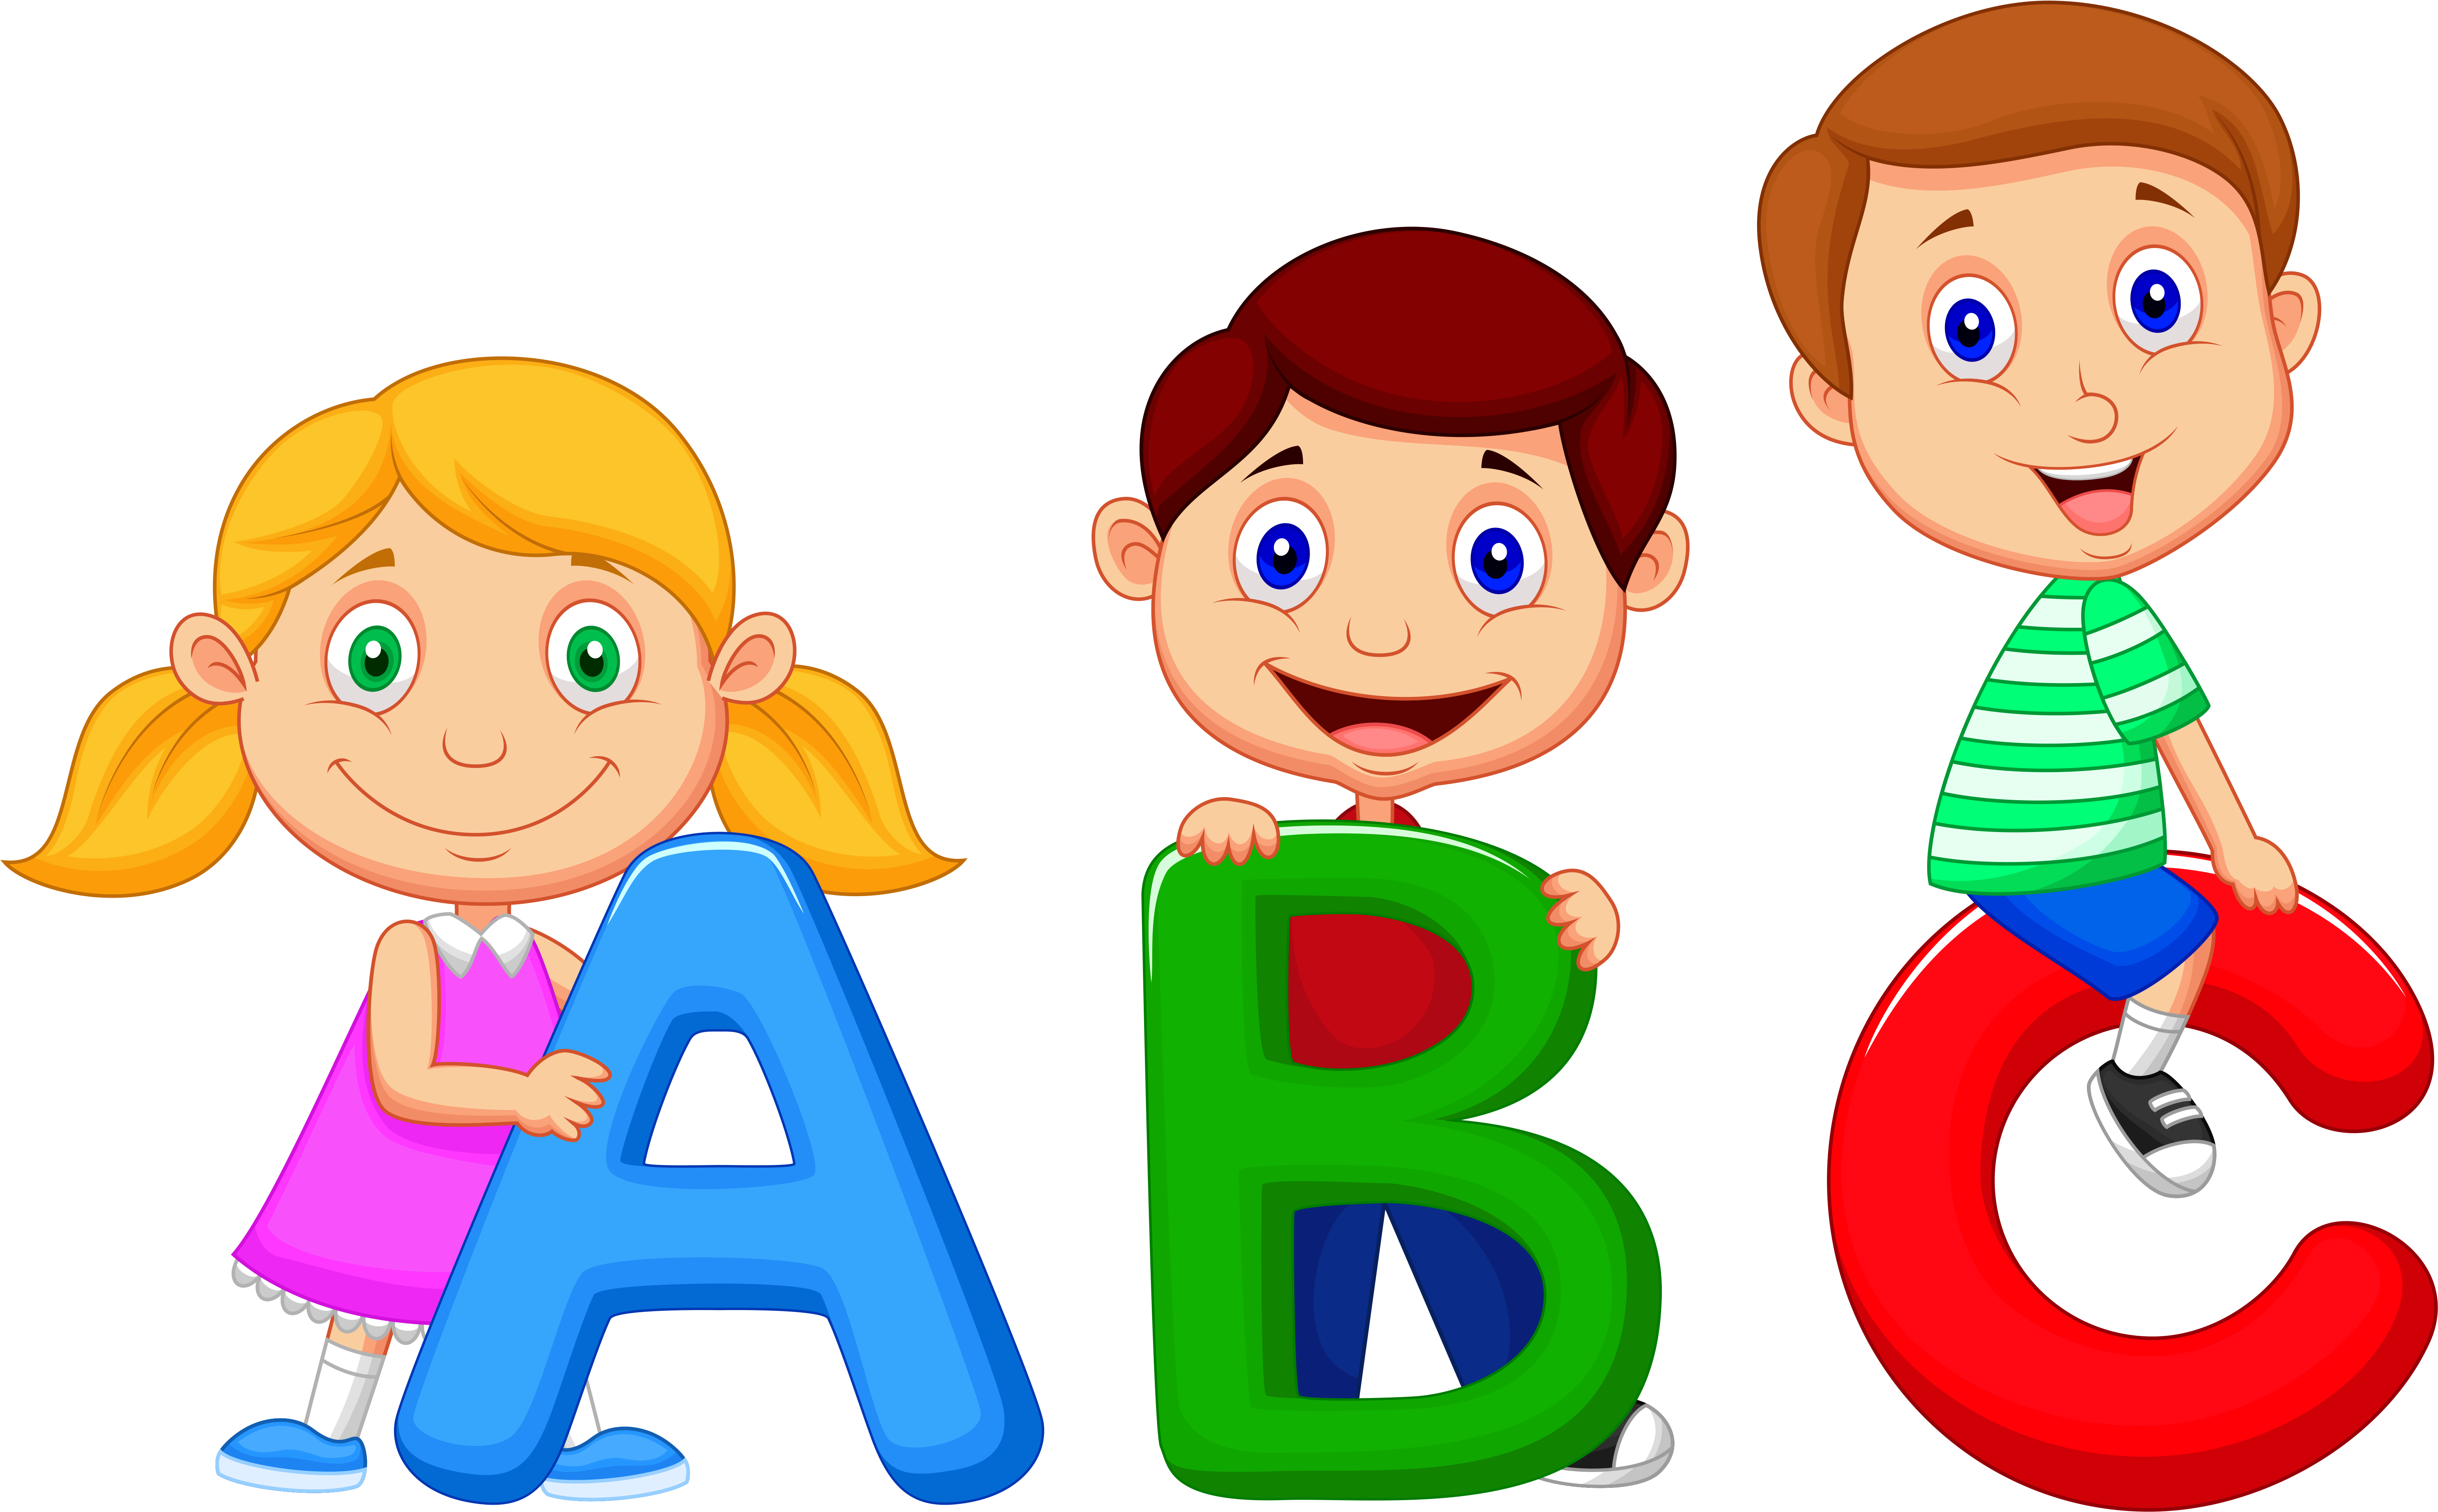
\includegraphics[width=1\textwidth,height=\textheight]{./pictures/clipart145720.png}}

}

\end{figure}

\bookmarksetup{startatroot}

\hypertarget{sec-vorwort}{%
\chapter*{Vorwort}\label{sec-vorwort}}
\addcontentsline{toc}{chapter}{Vorwort}

\markboth{Vorwort}{Vorwort}

Dieses Buch enthält Begleittexte und Übungsvorschläge für das
Studienfach \emph{Spracherwerb} (sl. \emph{Usvajanje jezika}, en.
\emph{Language acquisition}), das im Rahmen des Germanistikstudiums an
der Universität Maribor als Wahl- und Pflichtfach angeboten wird.

Das Buch wurde mit Hilfe der Programmierungssprache \texttt{R}
\url{https://www.r-project.org/} und der von \texttt{RStudio}
\url{https://www.rstudio.com/} entwickelten Skriptsprache
\texttt{Rmarkdown} \url{https://rmarkdown.rstudio.com/} auf der
Entwickler-Platform \texttt{Github} \url{https://github.com/} als
\texttt{Quarto\ Book} \url{https://quarto.org/} veröffentlicht.

\part{Grundlagen}

\hypertarget{sec-einfuhrung}{%
\chapter{Einführung}\label{sec-einfuhrung}}

In diesem Buch besprechen wir Entwicklungsabläufe, Tendenzen und
Paradigmen im Erst- und Zweit-/Fremdspracherwerb des Deutschen
(teilweise auch im Slowenischen), die im Rahmen verschiedener
Forschungsbereiche (Psycho- und Neurolinguistik, Spracherwerb,
Sprachvarietäten, \ldots) diskutiert werden und auch für germanistische
Studien von Interesse sein können. Die verwendeten Methoden und
praktischen Aufgaben sind zum Teil verallgemeinerbar und übertragbar auf
andere intellektuelle Arbeitsbereiche.\footnote{Dieses Buch wurde mit
  \texttt{Quarto} \url{https://quarto.org/docs/books/} zusammengestellt.}

Die vorgesehenen \emph{Themenbereiche}:\\

\begin{itemize}
\tightlist
\item
  Leitfragen in der Spracherwerbsforschung,\\
\item
  Merkmale verschiedenener Spracherwerbstypen,\\
\item
  Vor- und Nachteile der Mehrsprachigkeit,\\
\item
  Neurobiologische und kognitive Grundlagen des Spracherwerbs,\\
\item
  Markante Thesen einflussreicher Spracherwerbstheorien,\\
\item
  Spracherwerbsstadien am Beispiel deutscher Kinder,\\
\item
  Entwicklungsverläufe und Paradigmen am Beispiel deutscher
  Spracherwerbskorpora,\\
\item
  Sprachproduktion und -rezeption im Zweit-/Fremdspracherwerb,\\
\item
  Entwicklungsbedingte und transferbedingte sprachliche Konstruktionen
  im Zweit-/Fremdspracherwerb (v.a. am Beispiel slowenischer
  Lernender).\\
\end{itemize}

In diesem Einführungskurs machen wir Sie mit einigen der grundlegenden
Methoden zur Erfassung der linguistischen Merkmale in deutschen (und in
einigen Abschnitten auch mit slowenischen) Texten bekannt.

Hinweise\footnote{Clipart von \url{https://www.clipartmax.com/}}:

Das ist eine Definition (rmdnote).

Das ist ein Tip oder eine Info (rmdtip).

Das ist ein Arbeitsvorschlag (rmdrobot).

Das ist der RStudio Logotyp (rmdrstudio).

Das ist eine Warnung (rmdwarning).

Das ist eine Fehlermeldung (rmderror).

\hypertarget{sec-gegenstand}{%
\chapter{Leitfragen in der
Spracherwerbsforschung}\label{sec-gegenstand}}

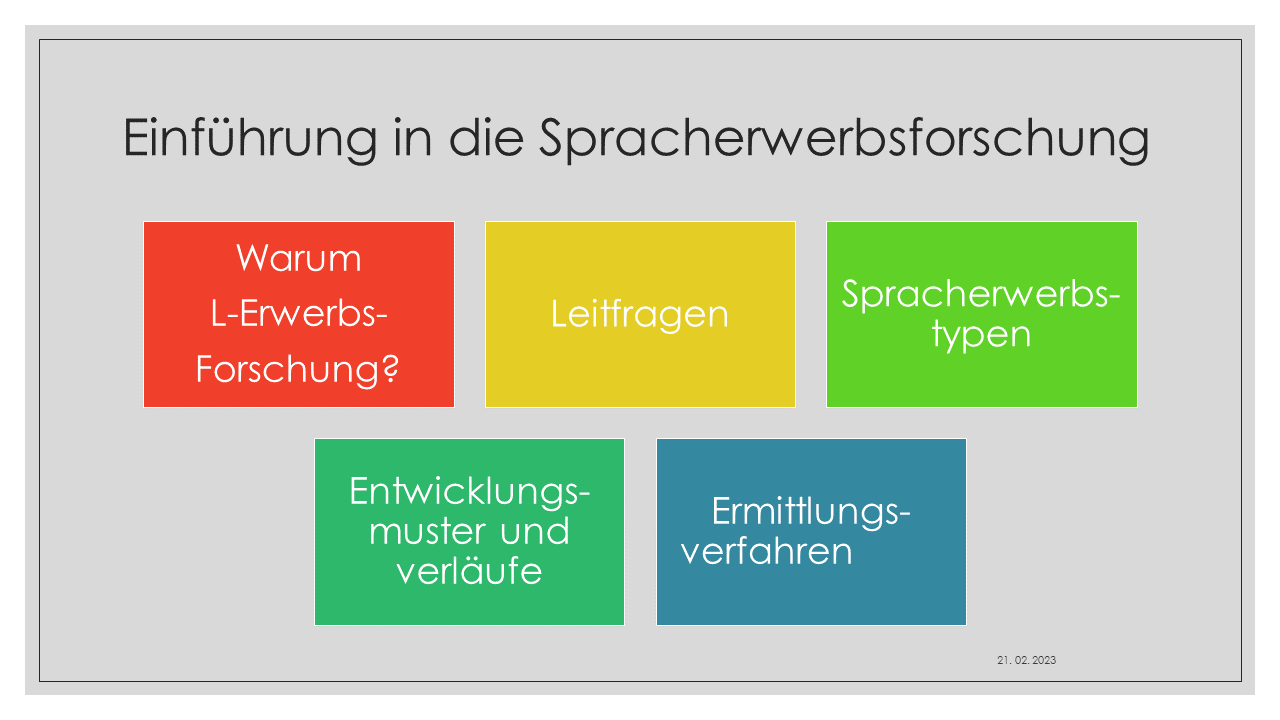
\includegraphics[width=1\textwidth,height=\textheight]{./pictures/UJ_Intro_2023_02.png}

Die Kernthemen der Spracherwerbsforschung lassen sich gemäß Kauschke
(2012) anhand von drei \textbf{Grundfragen} umreißen:

1. Was macht sprachliches Wissen, was macht die Beherrschung einer
Sprache aus?

2. Ist sprachliches Wissen angeboren oder wird es erlernt?

3. Wird Sprache über sprachspezifische oder über allgemein-kognitive
Mechanismen erworben?

\hypertarget{sprachbeherrschung}{%
\section{Sprachbeherrschung}\label{sprachbeherrschung}}

\textbf{Begriff des sprachlichen Wissens}

Sprache ist Bestandteil der menschlichen \textbf{Kognition}: Prozesse
der mentalen Speicherung, Aufnahme und Verarbeitung von Informationen.

Diesen Prozessen kann das \textbf{Bewusstsein} zugeschaltet sein oder
nicht.

Menge der gespeicherten Informationen (\textbf{deklaratives Wissen},
auch »Wissen, dass«)

Verfügbarkeit von informationsverarbeitenden Prozessen
(\textbf{prozedurales Wissen}, auch »Wissen, wie«).

Was macht nun sprachliches Wissen in diesem Sinne aus? Versteht man
Sprache als \textbf{gegliedertes System} von Einheiten, die durch ihre
Analysierbarkeit und ihre Kombinierbarkeit gekennzeichnet sind, so
bildet die \textbf{Entwicklung der Fähigkeit, sprachliche Einheiten zu
segmentieren und miteinander zu kombinieren, den Kern des
Spracherwerbs}.

Über den Aufbau sprachstrukturellen Wissens hinaus ist Wissen über die
\textbf{Gebrauchsbedingungen} von Sprache, ihre kommunikative Funktion
und ihren reziproken Charakter ebenfalls Gegenstand des Spracherwerbs.
Derartige anwendungsbezogene Aspekte von Sprache werden bereits
\textbf{im ersten Lebensjahr} in Austauschprozessen zwischen dem Kind
und seinen \textbf{Bezugspersonen} angebahnt und im weiteren Verlauf
ausdifferenziert.

\hypertarget{ist-sprachliches-wissen-angeboren-oder-wird-es-erlernt}{%
\section{Ist sprachliches Wissen angeboren oder wird es
erlernt?}\label{ist-sprachliches-wissen-angeboren-oder-wird-es-erlernt}}

Seit langem als Kernthema der Spracherwerbsforschung und immer wieder
neu diskutiert. Debatte um den Einfluss von Erbe und Umwelt auf die
Entwicklung von Individuen. Ausbildung dieser humanspezifischen
Fähigkeit nur möglich, wenn die sprachlernenden Menschen einer
Umgebungssprache ausgesetzt sind. Kontrovers wird diskutiert, welche
Rolle und welches Gewicht anlagebedingten Faktoren auf der einen Seite
und dem Sprachangebot der Umwelt auf der anderen Seite zukommt. Kommt
das Kind vorgeprägt für Sprache auf die Welt, ausgestattet mit
spezifischen Fähigkeiten, die in der menschlichen Entwicklungsgeschichte
entstanden sind? Entwickelt sich Sprache gemäß angeborener innerer
Voraussetzungen und vorgeprägter Reifungsprozesse entwickelt. Geht man
dagegen davon aus, dass das Kind Sprache aktiv und vorrangig durch
Kontakt und Kommunikation mit anderen Sprechern lernt.  

\hypertarget{domuxe4nenspezifik-von-sprache.}{%
\section{Domänenspezifik von
Sprache.}\label{domuxe4nenspezifik-von-sprache.}}

Wird Sprache über sprachspezifische oder allgemein-kognitive Mechanismen
erworben? Denkbar ist, dass allgemeine kognitive Prozesse auf
verschiedene Wissens- und Aufgabenbereiche anwendbar sind.

Eine andere Position besteht in der Annahme, dass für den Spracherwerb
domänenspezifisches Wissen notwendig ist, das darauf spezialisiert ist,
nur einen bestimmten Typus von Informationen zu verarbeiten.

In der Spracherwerbsforschung lassen sich drei große, traditionelle
Erklärungsparadigmen unterscheiden:

\begin{itemize}
\tightlist
\item
  Nativismus,
\item
  Interaktionismus und
\item
  Kognitivismus.
\end{itemize}

Neuere Erklärungsmodelle arbeiten auf eine Synthese hin.

\hypertarget{sec-zungenbrecher}{%
\chapter{Spracherwerbstypen}\label{sec-zungenbrecher}}

\begin{figure}

{\centering 

\href{https://www.clipartmax.com/middle/m2i8K9K9N4m2A0A0_fall-leaves-clip-art-september-writing/}{
\includegraphics[width=1\textwidth,height=\textheight]{./pictures/clipart49430.png}}

}

\end{figure}

\hypertarget{terminologische-unterscheidung}{%
\section{Terminologische
Unterscheidung}\label{terminologische-unterscheidung}}

In der Sprachewerbsforschung ist es möglich und üblich, verschiedene
Verben und Nomina zu verwenden, um auf verschiedene Spracherwerbstypen
Bezug zu nehmen.

\emph{Verben}: (eine Sprache) erwerben, sich (eine Sprache) aneignen,
(eine Sprache) lernen.

\emph{Nomina}: der Erwerb einer Sprache, die Aneignung einer Sprache,
das Lernen einer Sprache.

Welche semantischen Unterschiede bestehen zwischen den genannten Verben
und Nomina?

Vorschlag: Schauen Sie mal im \emph{DWDS} \url{https://www.dwds.de/}
nach und versuchen Sie festzustellen, in welchen Kontexten die Verben /
Nomina vorkommen!

Vergleichen Sie die Bedeutungen auch mit den Bedeutungen entsprechender
slowenischer und englischer Ausdrücke:

\emph{Slowenisch}: pridobiti (jezik), usvojiti (jezik), se učiti
(jezika).\\
\emph{Englisch}: acquire, learn (a language), \ldots{}

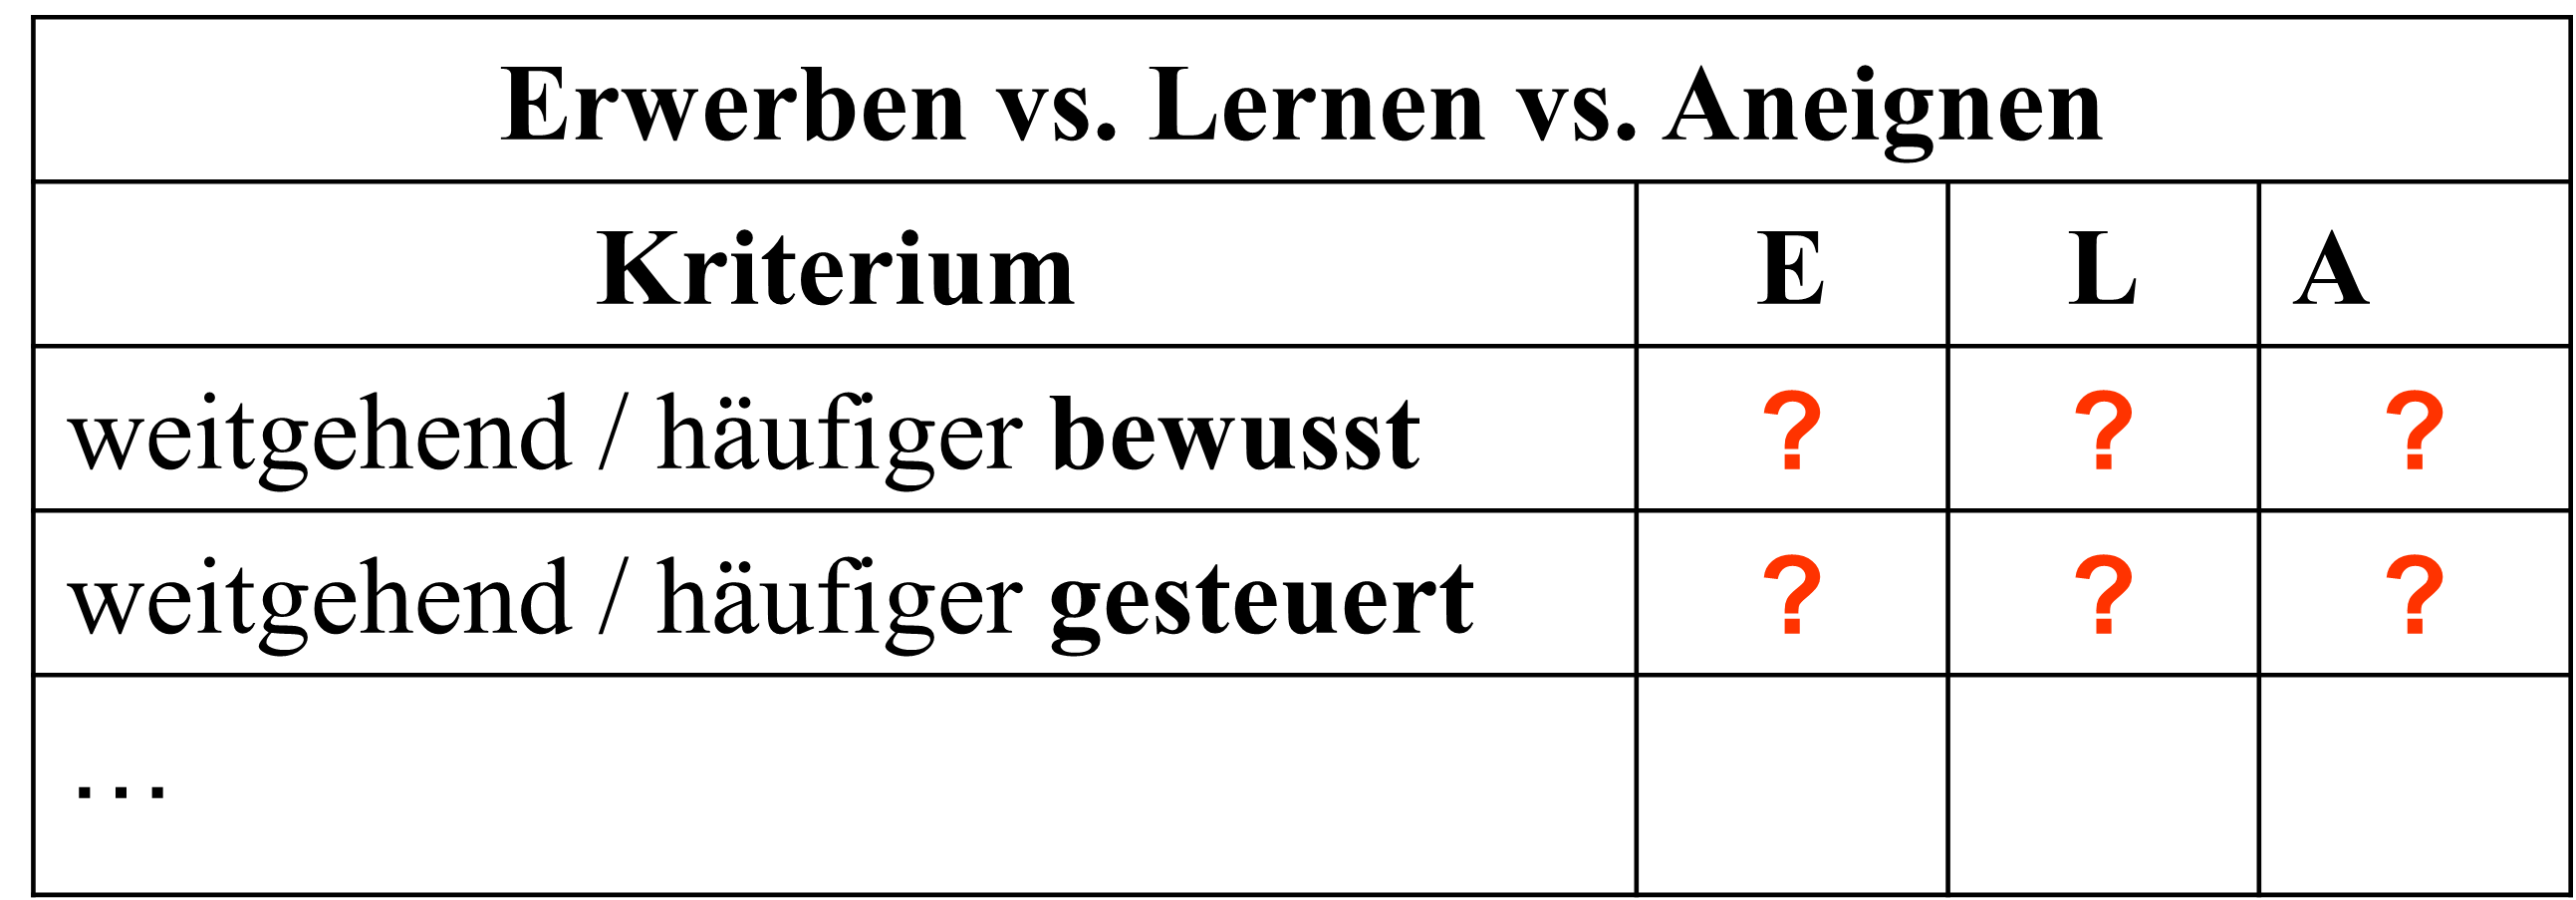
\includegraphics[width=8.62in,height=\textheight]{./pictures/termini_verben_nomen.png}

\emph{Aneignung} (A) soll als \emph{Oberbegriff} für Erwerb und Lernen
dienen. Die Aneignung einer Erstsprache ist stärker von
\emph{Erwerbsprozessen} geprägt. Die Aneignung einer Fremdsprache ist
stärker von \emph{Lernprozessen} geprägt. Die Aneignung einer
Zweitsprache (im engeren Sinne) ist je nach Fall stärker von
\emph{Erwerbs}- bzw. \emph{Lern}prozessen geprägt.

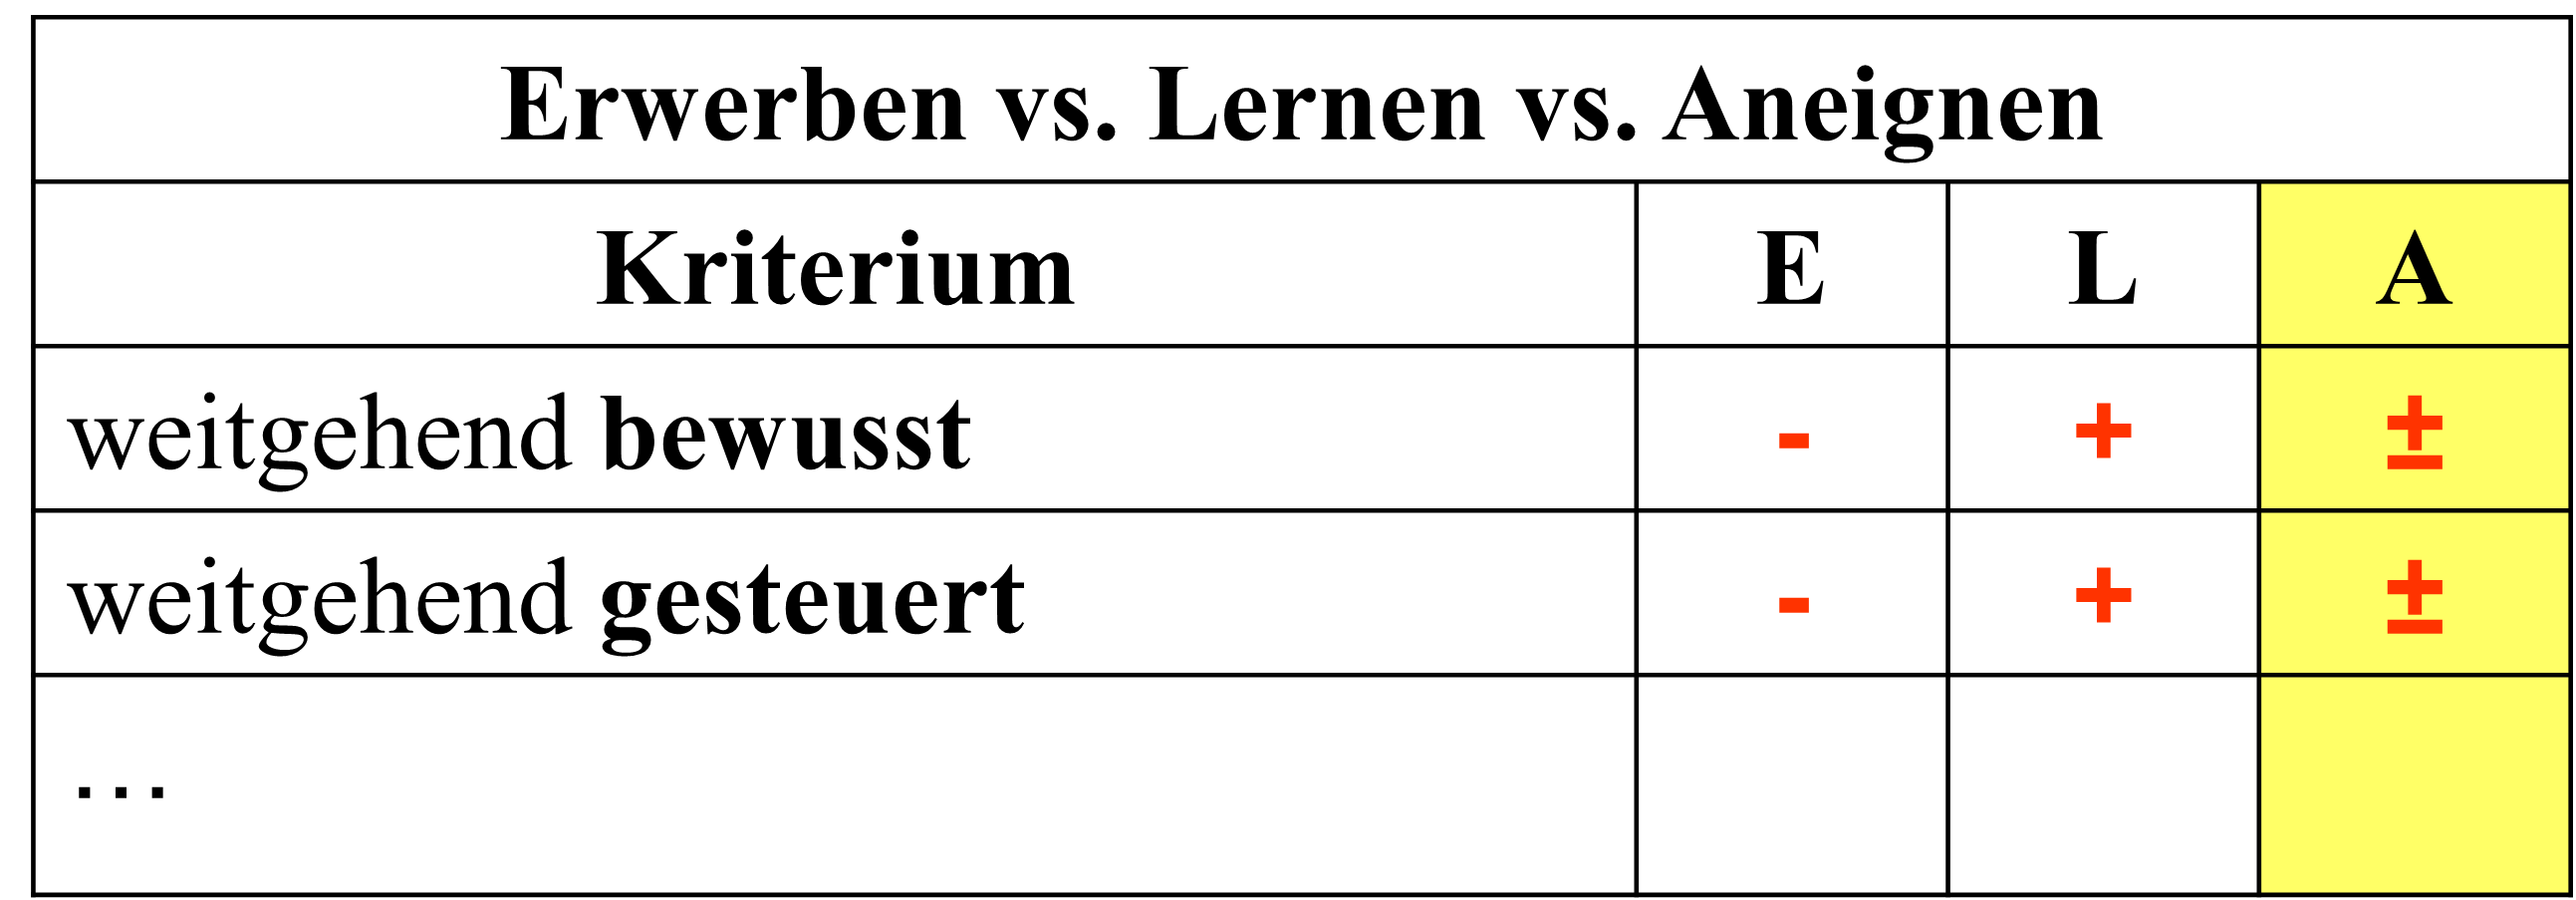
\includegraphics[width=8.62in,height=\textheight]{./pictures/termini_verben_nomen2.png}

Ihnen werden nun ein paar Videoausschnitte gezeigt, in denen die Art und
Weise beschrieben wird, wie sich Menschen eine Sprache aneignen.

Versuchen Sie, die wesentlichen Unterschiede und eventuelle
Gemeinsamkeiten herauszufinden !

\href{https://www.youtube.com/watch?v=cS_aH5wJGME}{Easy German} (Dauer:
11:07 Minuten):

\url{https://www.youtube.com/embed/cS_aH5wJGME}

\hypertarget{unterscheidungskriterien}{%
\section{Unterscheidungskriterien}\label{unterscheidungskriterien}}

Wir können eine Reihe von Kriterien verwenden, um drei
Spracherwerbstypen zu unterscheiden.

\emph{L1} steht für \emph{Erstsprache} (oft auch als
\emph{Muttersprache} bezeichnet), \emph{L2} bezieht sich auf die
\emph{Zweitsprache} und\\
\emph{FL} wird in der Tabelle für \emph{Fremdsprache} verwendet.

Der Ausdruck \emph{Muttersprache} ist bei bilingualen (d.h.
zweisprachigen) Personen nicht unbedingt zutreffend (\emph{warum?}),
darum ist \emph{Erstsprache} als Fachterminus zu bevorzugen.

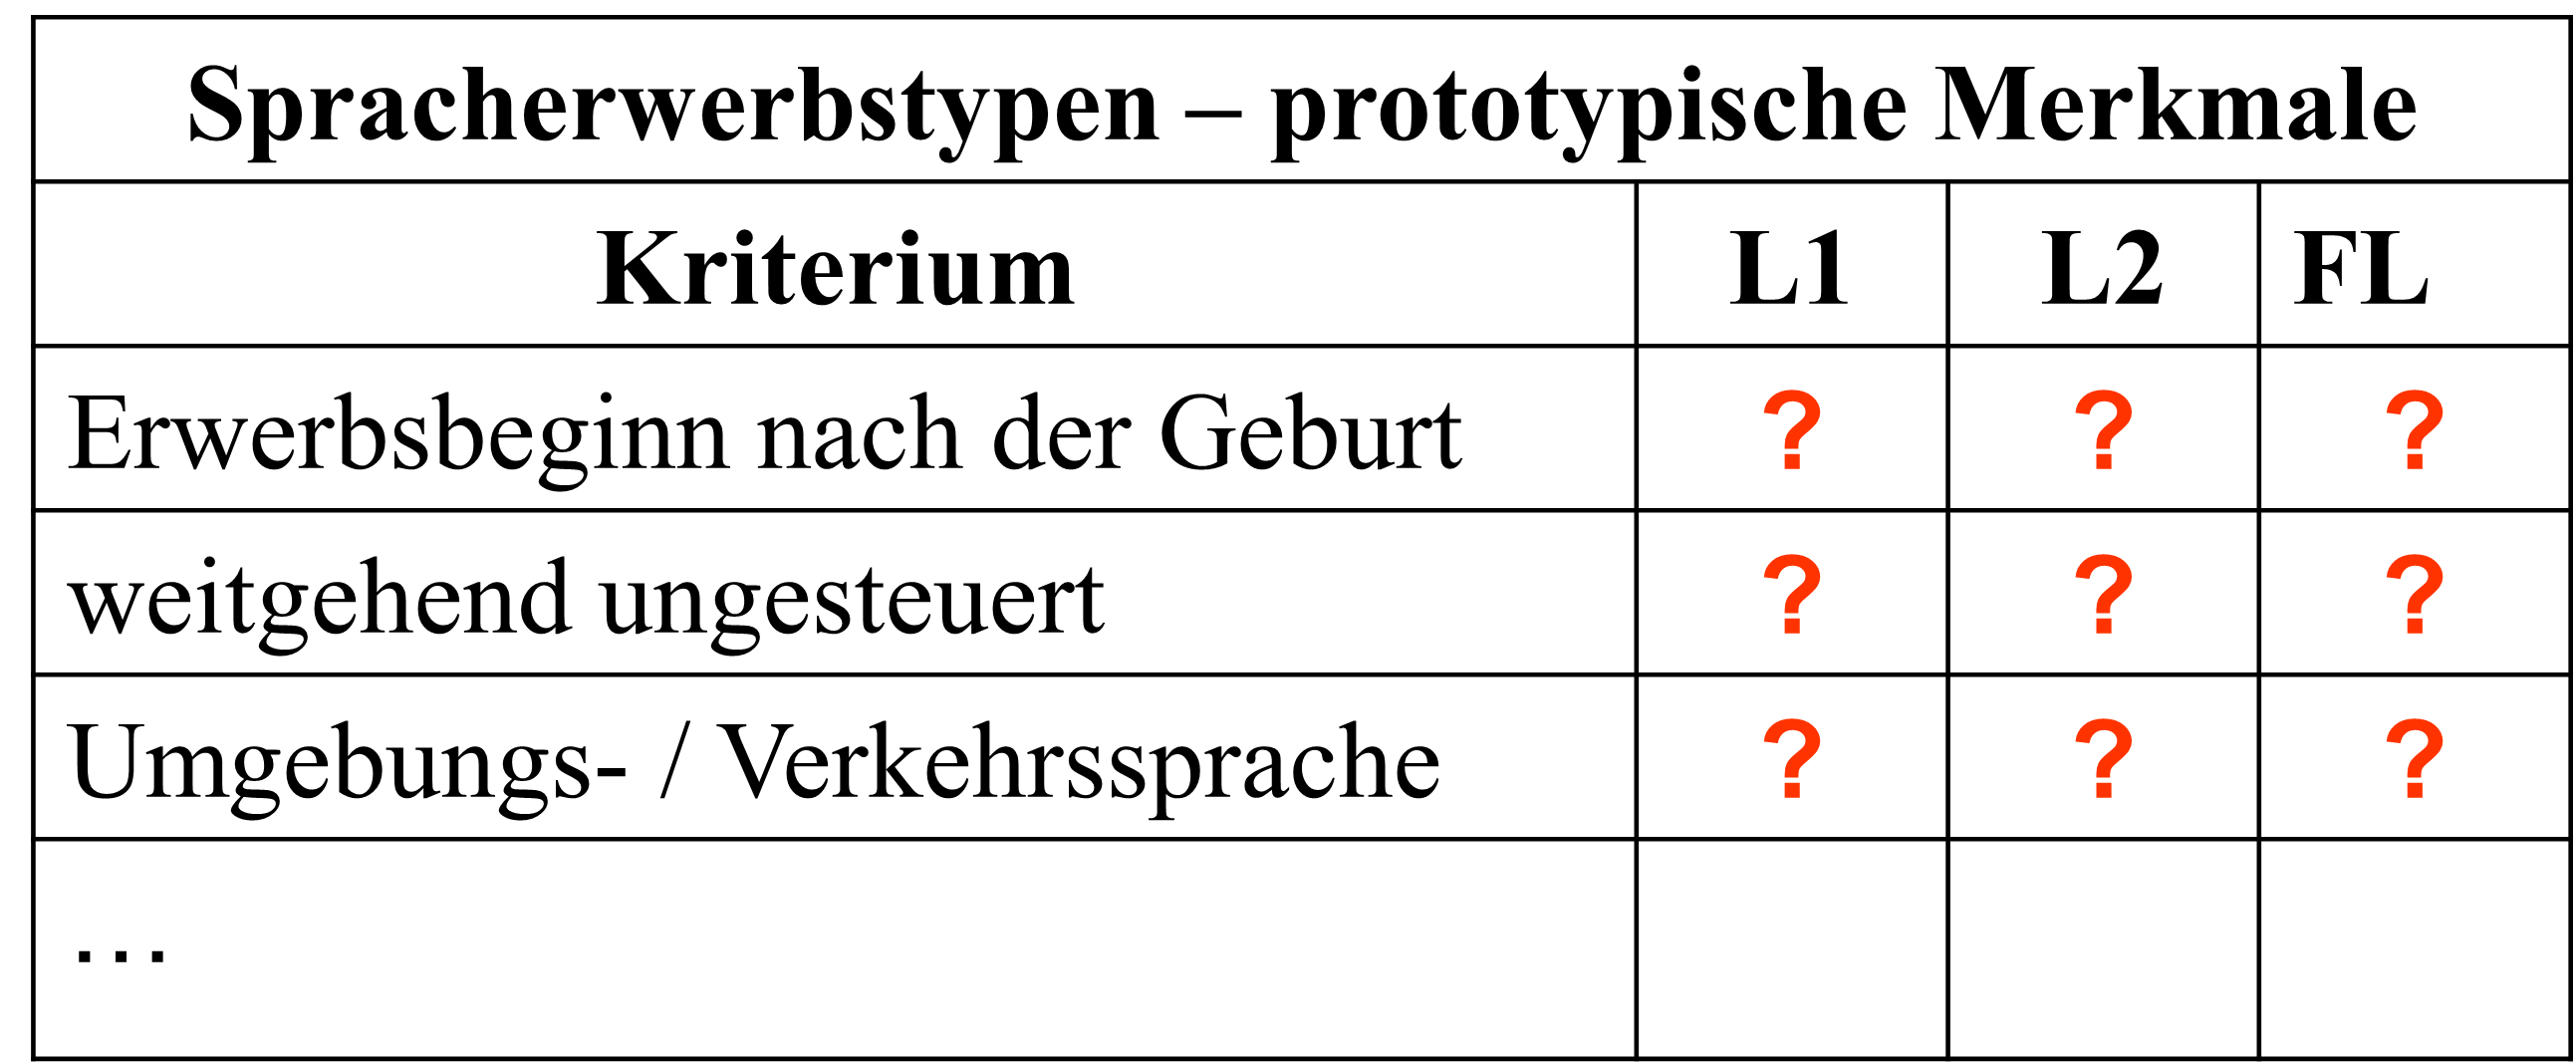
\includegraphics[width=8.62in,height=\textheight]{./pictures/spracherwerbstypen.png}

Ihnen werden nun ein paar Videoausschnitte gezeigt, in denen die Art und
Weise beschrieben wird, wie sich Menschen eine Sprache aneignen.

Versuchen Sie, die wesentlichen Unterschiede und eventuelle
Gemeinsamkeiten herauszufinden !

\href{https://www.youtube.com/watch?v=ZqObBG-NYPI}{Easy German} (Dauer:
8:46 Minuten):

\url{https://www.youtube.com/embed/ZqObBG-NYPI}

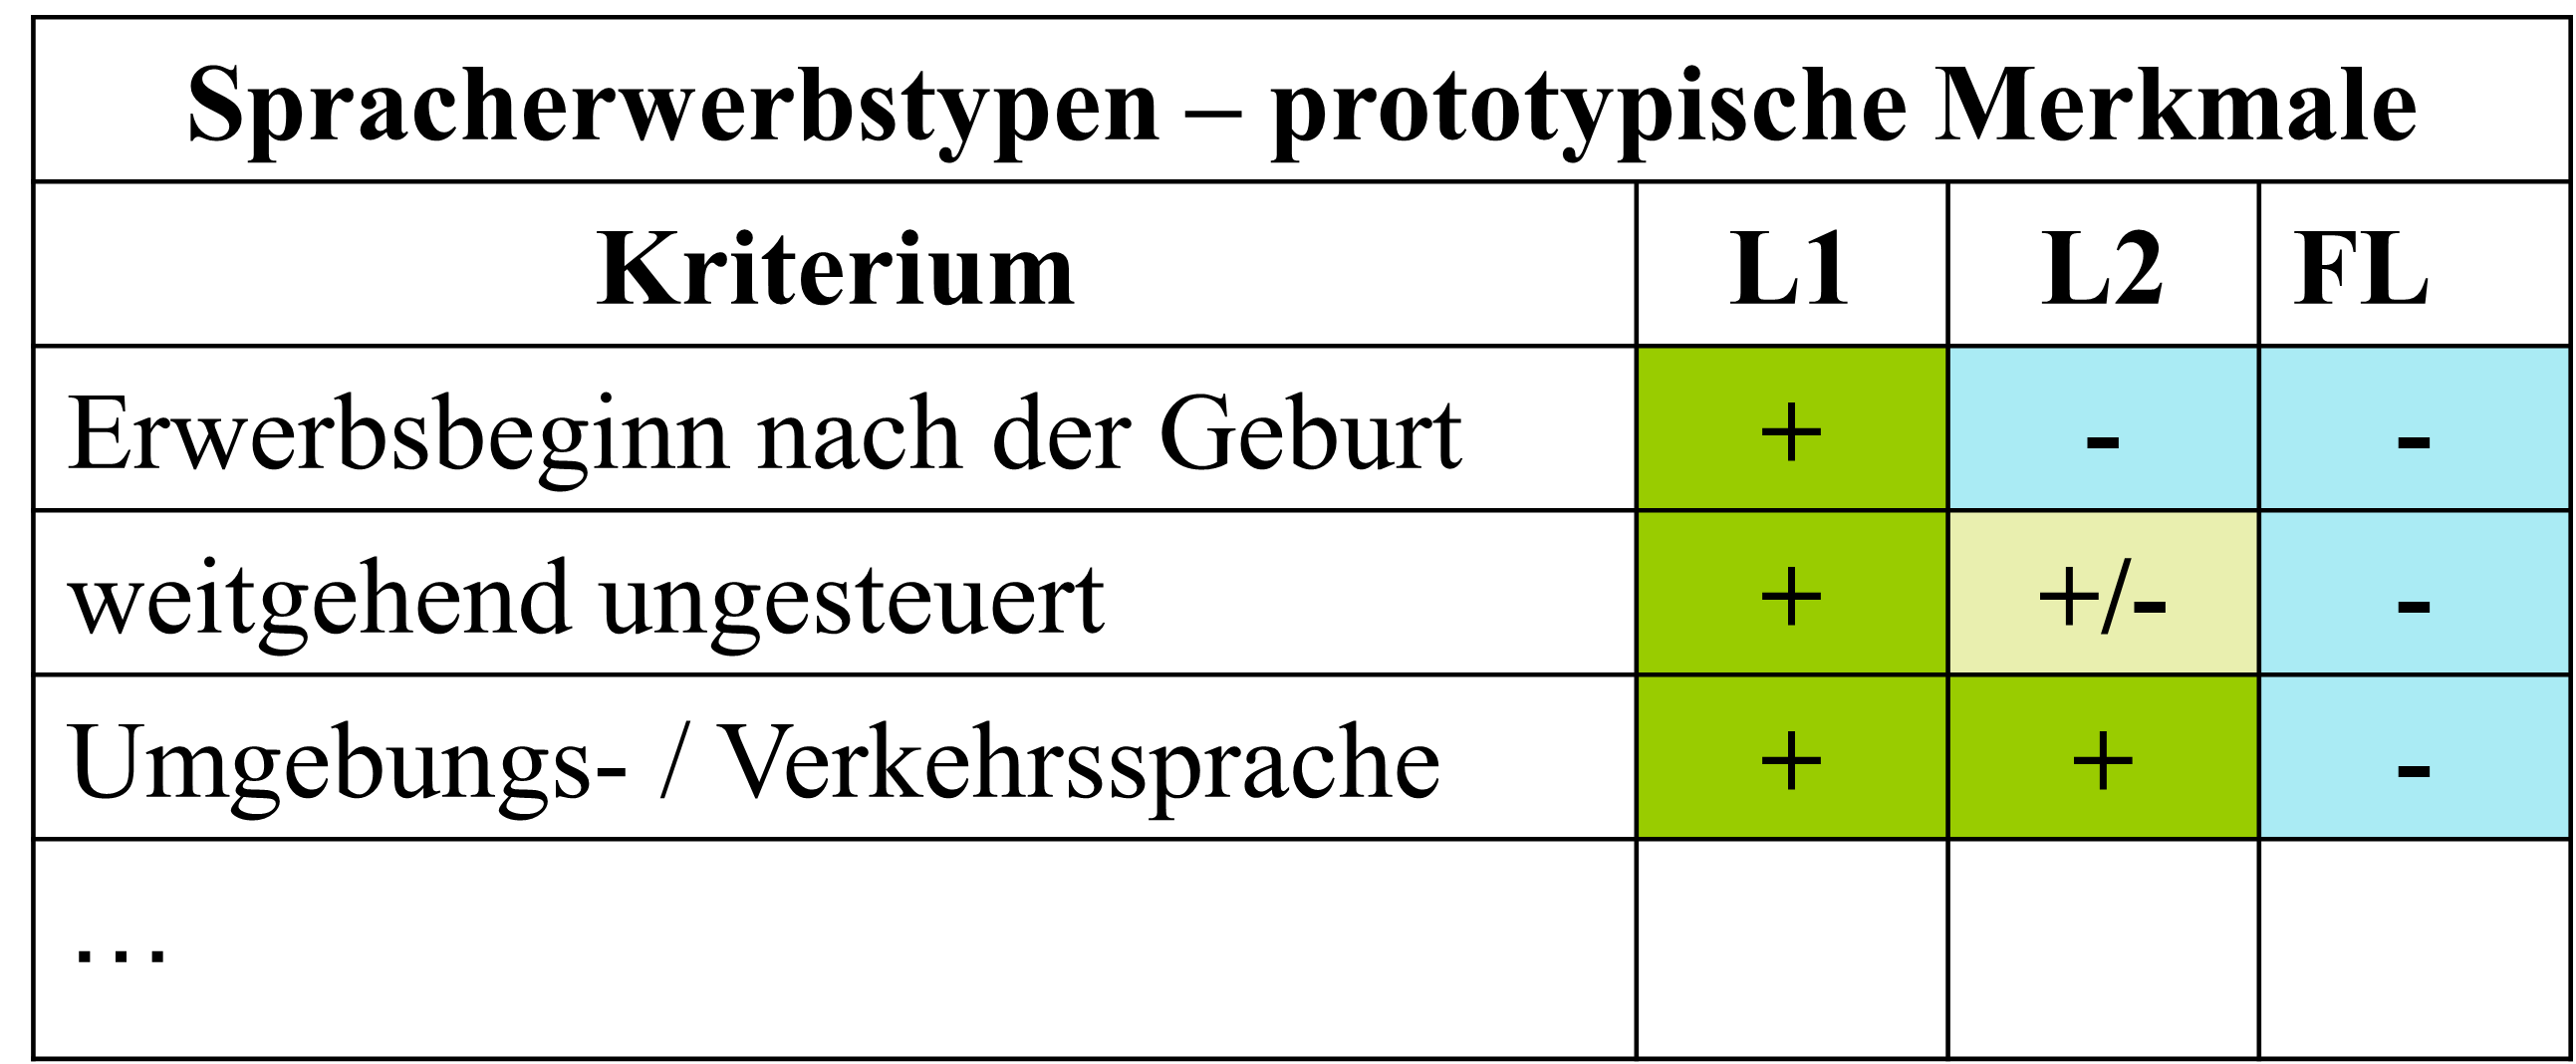
\includegraphics[width=8.62in,height=\textheight]{./pictures/spracherwerbstypen2.png}

In der Forschungsliteratur wird der Begriff \textbf{Zweitspracherwerb}

\begin{itemize}
\item
  \emph{im engeren Sinne} (wie in der zuvor gezeigten Tabelle),
\item
  bisweilen aber auch \emph{im weiteren Sinne} verwendet.
\end{itemize}

Im zweiten Fall werden Fremdspracherwerb und Zweitspracherwerb (im
engeren Sinne) als Zweitspracherwerb \textbf{zusammengefasst}. Welche
wichtige \textbf{Gemeinsamkeit} ist dafür wohl \textbf{ausschlaggebend}
?

Der Erstspracherwerb kann auch in der Form eines \textbf{doppelten
Erstspracherwerbs} (oder mehrfachen L1-Erwerbs) vorkommen.

Im Fall von bilingulaen Personen ist es auch aus neurobiologischer
Perspektive sinnvoll, zwischen \textbf{frühem} und \textbf{späten
Bilingualismus} zu unterscheiden.

\hypertarget{sec-bilingual}{%
\chapter{Vor- und Nachteile der Mehrsprachigkeit}\label{sec-bilingual}}

\begin{figure}

{\centering 

\href{https://www.clipartmax.com/middle/m2H7m2i8Z5A0N4Z5_lounge-style-sunglasses-retro-interlude-png-image-high-glasses-clipart-retro/}{
\includegraphics[width=1\textwidth,height=\textheight]{./pictures/clipart4776991.png}}

}

\end{figure}

Zwei- oder Mehrsprachigkeit hat nach Ansicht vieler Menschen mehrere
Vorteile. Aber viele Menschen wachsen nicht zwei- oder mehrsprachig auf.
Deshalb erhebt sich nicht nur die Frage, welche Vorteile
Mehrsprachigkeit hat, sondern auch, ob es gewisse Nachteile gibt, die
Mehrsprachigkeitsbestreben hemmen oder sogar verhindern.

Hier folgt eine Liste von Behauptungen zur Mehrsprachigkeit. Beurteilen
Sie, welche Behauptungen Sie für richtig halten und welche für nicht
haltbar.

\emph{Mobilitätsaspekte}:

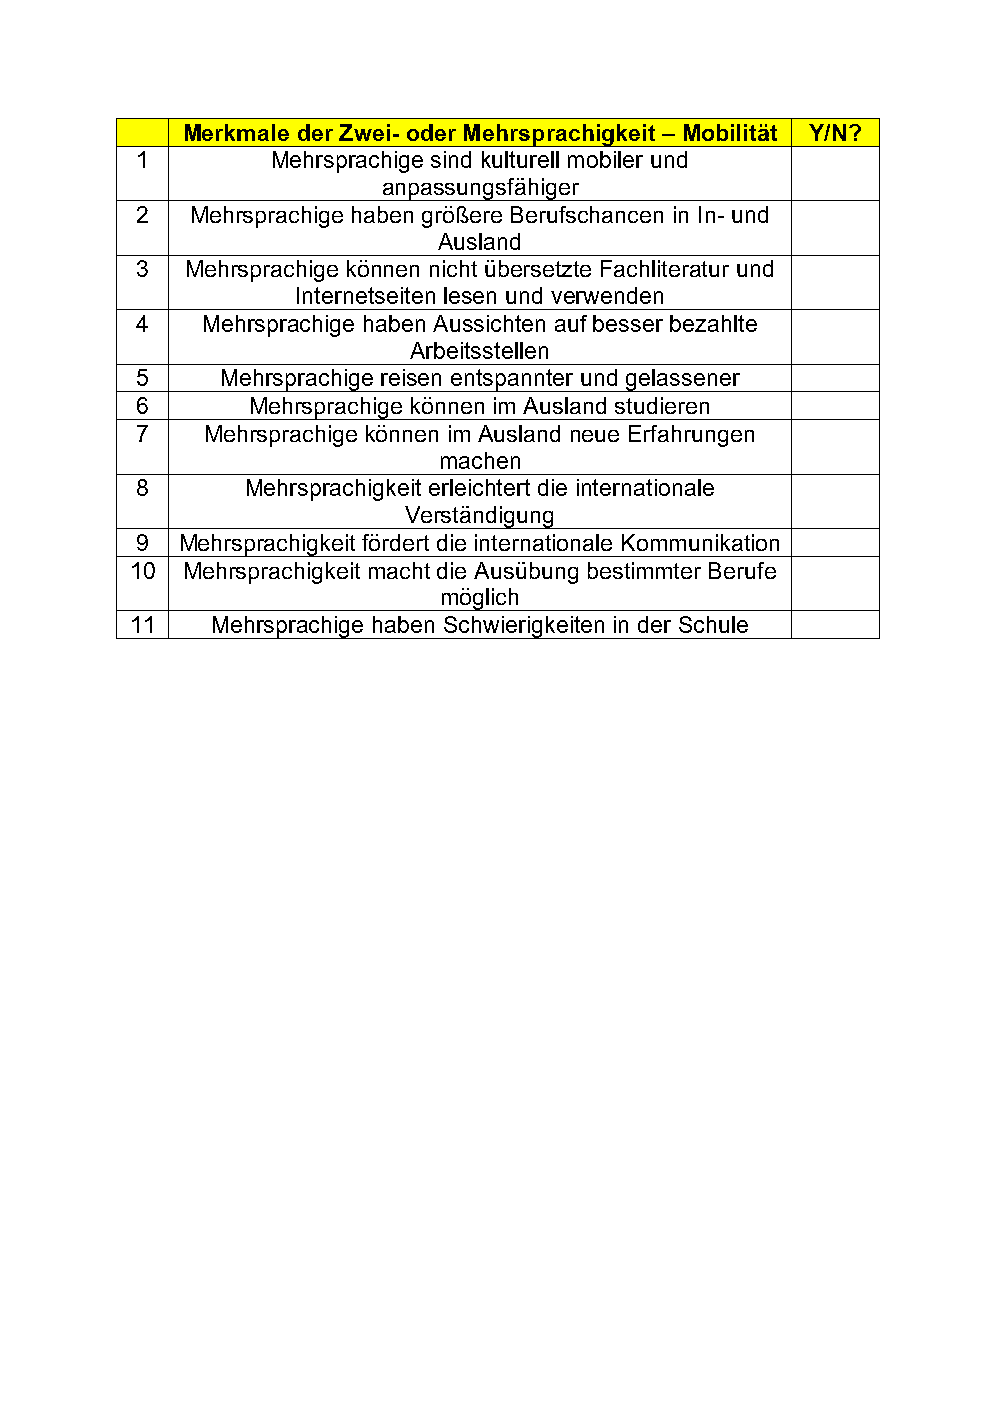
\includegraphics[width=3.31in,height=\textheight]{./pictures/Mehrsprachigkeit_Behauptungen_Page1.png}

\emph{Kulturelle Aspekte}:

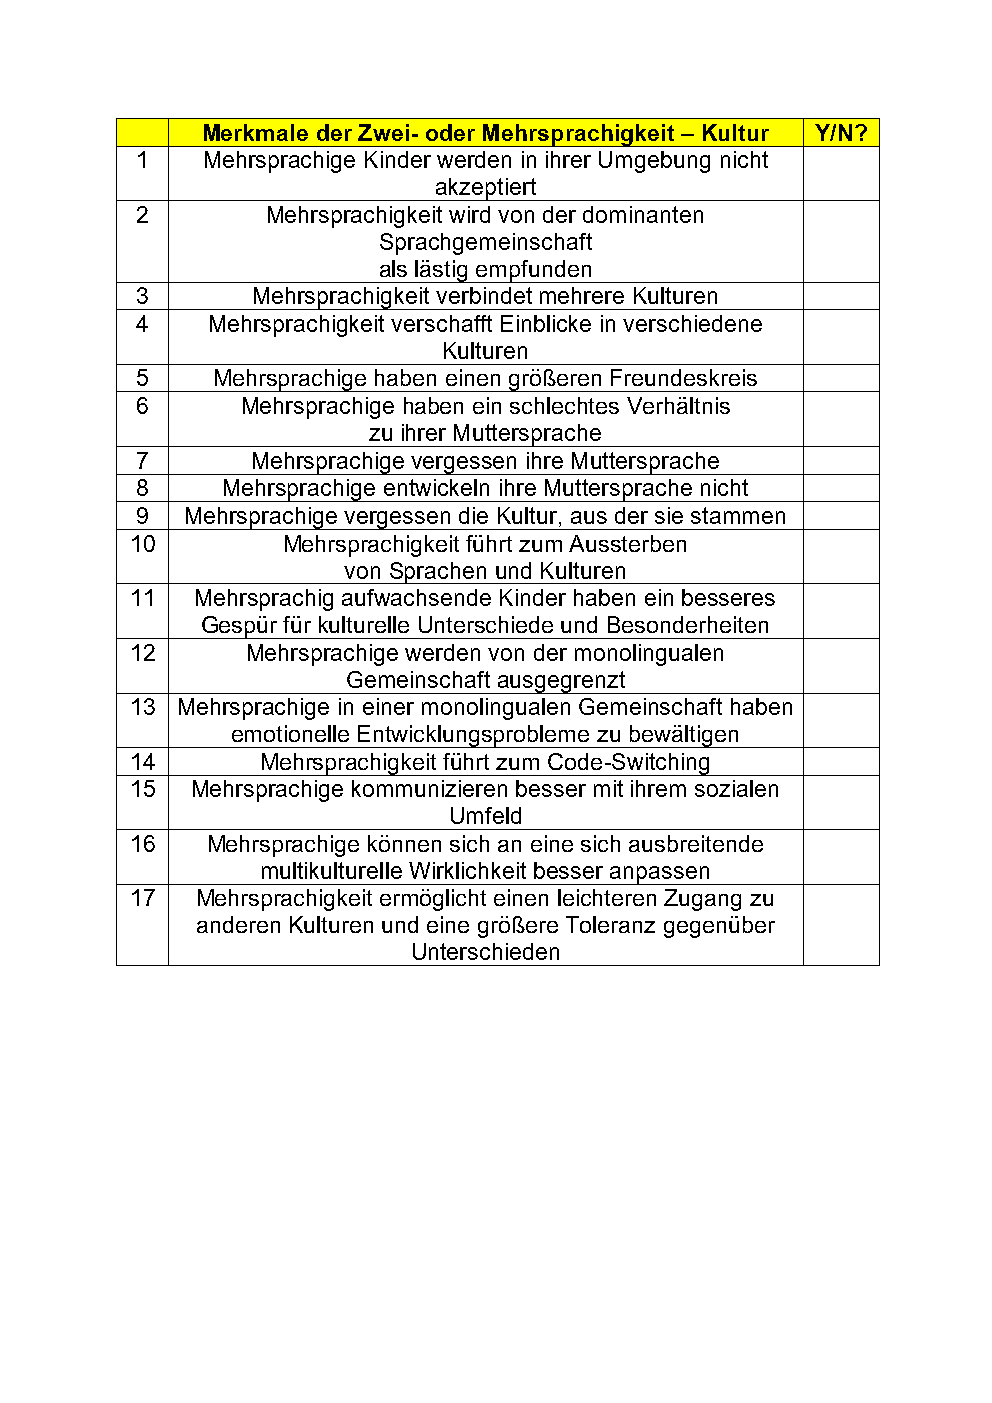
\includegraphics[width=3.31in,height=\textheight]{./pictures/Mehrsprachigkeit_Behauptungen_Page2.png}

\emph{Kognitive Aspekte}:

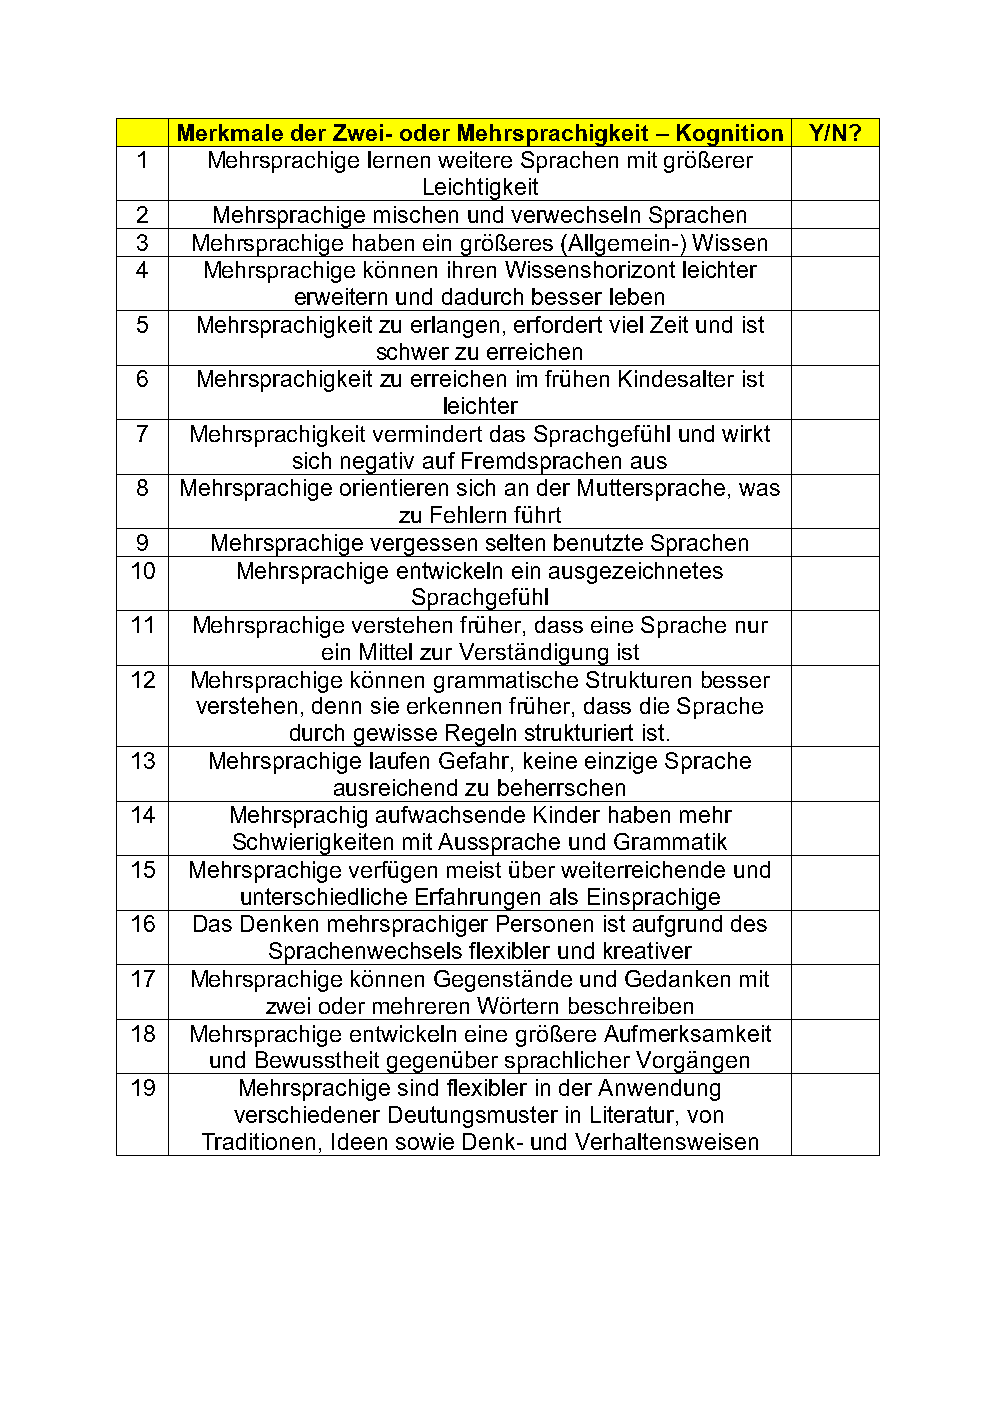
\includegraphics[width=3.31in,height=\textheight]{./pictures/Mehrsprachigkeit_Behauptungen_Page3.png}

In einem Artikel von \emph{Peter Ecke} Ecke (2008) werden \textbf{einige
Nachteile der Zwei- oder Mehrsprachigkeit} anhand von wissenschaftlichen
Studien diskutiert. Die Web-Adresse des Artikels:
\href{http://www.u.arizona.edu/~eckep/Ecke\%2008\%20Kosten\%20der\%20MS.pdf}{University
of Arizona}. Hier ist ein Abdruck der ersten Seite:

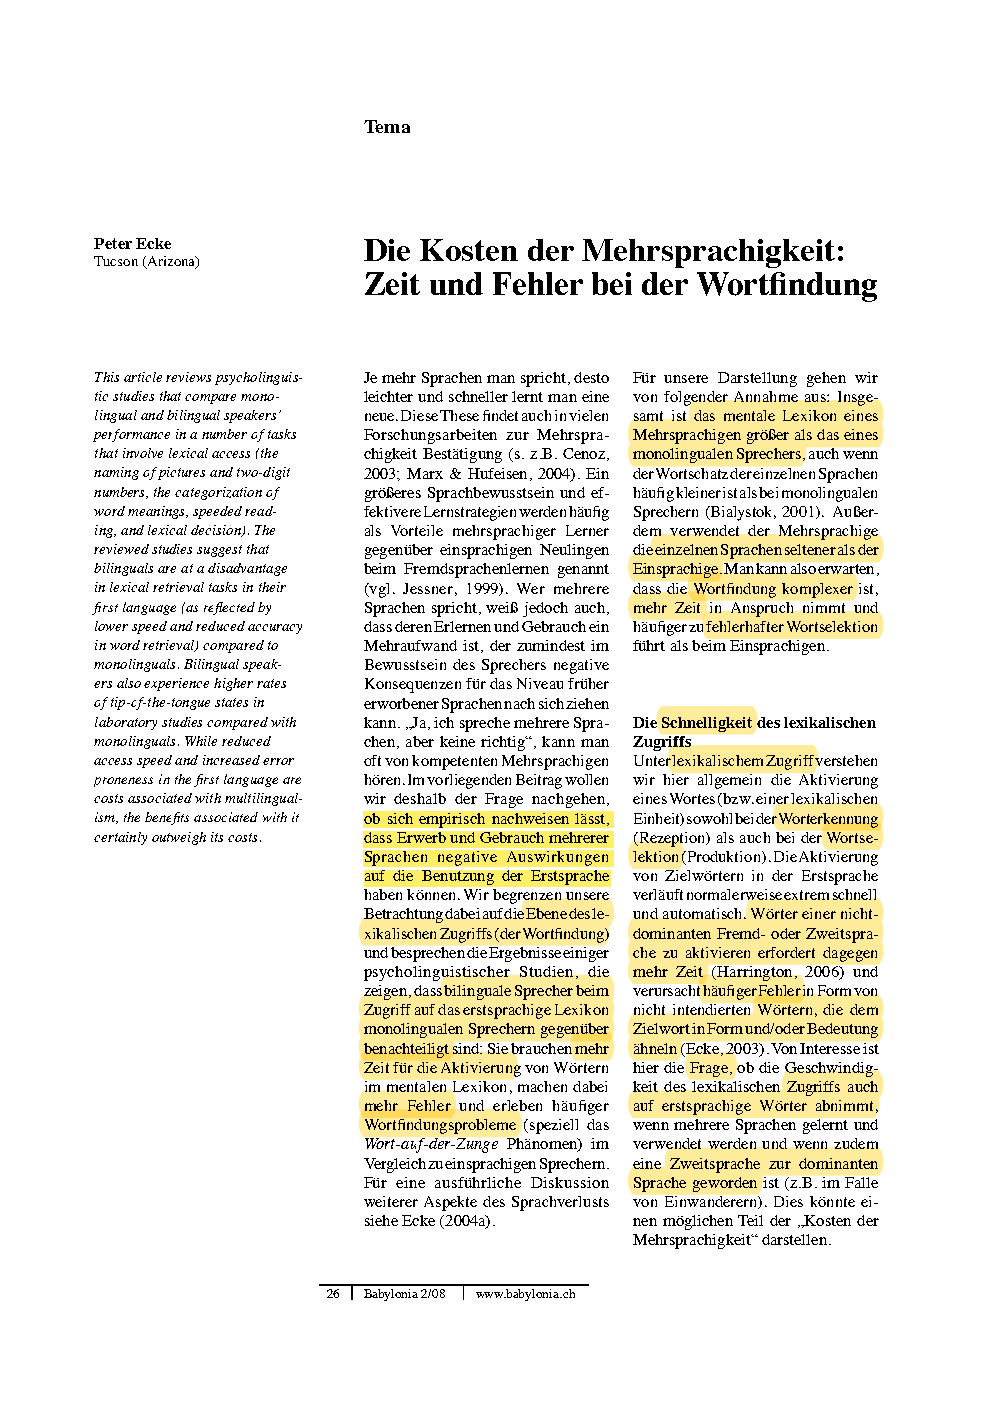
\includegraphics[width=3.31in,height=\textheight]{./pictures/TOT_bilangual_baby2_08ecke_annotated_Page1.png}

Ihnen werden nun Videos gezeigt, in denen Vorteile der
Zwei-/Mehrsprachigkeit und (vermeintliche) Nachteile erläutern werden.

Stellen Sie eine Liste der Vor- und Nachteile zusammen, damit Sie über
das Thema Mehrsprachigkeit diskutieren und entsprechend argumentieren
könen!

\href{https://www.youtube.com/watch?v=35XkRMBT28c}{Herzenssprache}
(Dauer: 7:53 Minuten):

\url{https://www.youtube.com/embed/35XkRMBT28c}

Ein weiteres Video zum Thema \emph{Mehrsprachigkeit}.

Stellen Sie eine Liste der Vor- und Nachteile zusammen, damit Sie über
das Thema Mehrsprachigkeit diskutieren und entsprechend argumentieren
könen!

\href{https://www.youtube.com/watch?v=0lJKipFitnA}{Wanderlust Monica}
(Dauer: 12:34 Minuten):

\url{https://www.youtube.com/embed/0lJKipFitnA}

Ein längeres Gespräch mit \emph{Prof.~Dr.~Jürgen Meisel} zum Thema
\emph{Mehrsprachigkeit}.

Stellen Sie eine Liste der Vor- und Nachteile zusammen, damit Sie über
das Thema Mehrsprachigkeit diskutieren und entsprechend argumentieren
könen!

\href{https://www.youtube.com/watch?v=a2Iw0jDkwYI}{Gabriel Gelman
Sprachheld} (Dauer: 43:53 Minuten):

\url{https://www.youtube.com/embed/a2Iw0jDkwYI}

Ein kürzeres Gespräch mit \emph{Prof.~Dr.~Rosemarie Tracy} über das
Thema \emph{Mehrsprachigkeit}.

Stellen Sie eine Liste der Vor- und Nachteile zusammen, damit Sie über
das Thema Mehrsprachigkeit diskutieren und entsprechend argumentieren
könen!

\href{https://www.youtube.com/watch?v=SAlTrh_76p0}{Universität Mannheim}
(Dauer: 10:51 Minuten):

\url{https://www.youtube.com/embed/SAlTrh_76p0}

Ein Vortrag von \emph{Prof.~Dr.~Rosemarie Tracy} über das Thema
\emph{Mehrsprachigkeit}.

\href{https://www.youtube.com/watch?v=vTK5-HSjbjs}{BildungsTV} (Dauer:
53:15 Minuten):

\url{https://www.youtube.com/embed/vTK5-HSjbjs}

Ein Vortrag von \emph{Prof.~Dr.~Rosemarie Tracy} über das Thema
\emph{Spracherwerb}.

\href{https://www.youtube.com/watch?v=prCbpoi-3KI}{BildungsTV} (Dauer:
1:04:48):

\url{https://www.youtube.com/embed/prCbpoi-3KI}

\hypertarget{sec-spracherwerb}{%
\chapter{Methoden in der
Spracherwerbsforschung}\label{sec-spracherwerb}}

\begin{figure}

{\centering 

\href{https://www.clipartmax.com/middle/m2i8K9i8K9m2i8A0_solutions-for-reducing-leadership-burnout-technology-doesn-t-work/}{
\includegraphics[width=1\textwidth,height=\textheight]{./pictures/clipart55029.png}}

}

\end{figure}

In jeder wissenschaftlichen Disziplin müssen Daten erhoben werden, um
Erklärungsansätze empirisch überprüfen zu können. Zu diesem Zweck werden
verschiedene Methoden eingesetzt, einen theoretischen Ansatz zu
falsifizieren. In Kauschke (2012): 6-22 werden verschiedene Verfahren
für die Gewinnung von Daten beschrieben, die in Untersuchungen zum
Erstspracherwerb eingesetzt werden. Viele davon finden jedoch auch in
Untersuchungen zum Zweit- und Fremdspracherwerb Anwendung.

Welche Methoden werden in Kauschke (2012) beschrieben?\\
Welche Anwendungsbereiche finden sie?\\
Welche Vor- und Nachteile zeigen sich bei ihrer Anwendung?

Stellen Sie eine Präsentation zum Thema zusammen und illustrieren Sie
sie auch mit Abbildungen und Beispielen, die Sie im Internet ausfindig
gemacht haben!

\begin{figure}

{\centering 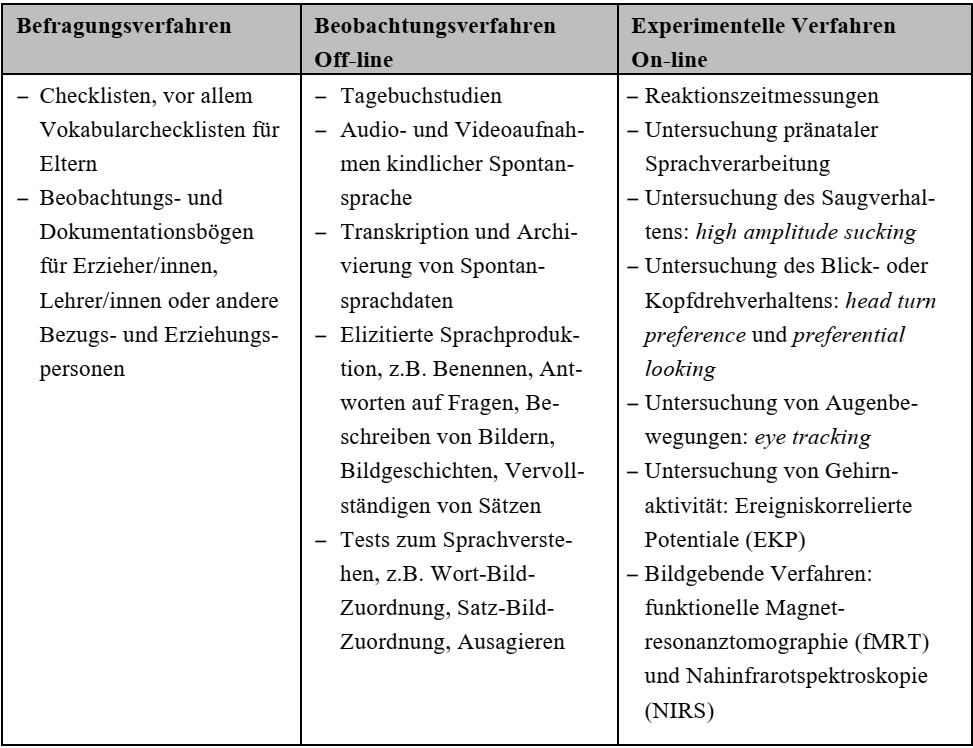
\includegraphics[width=1\textwidth,height=\textheight]{./pictures/methoden.png}

}

\caption{Übersicht über Methoden der Spracherwerbsforschung in Kauschke
(2012): 6}

\end{figure}

\hypertarget{sec-neuro}{%
\chapter{Neurobiologische und kognitive Grundlagen des
Spracherwerbs}\label{sec-neuro}}

\begin{figure}

{\centering 

\href{https://www.kissclipart.com/tongue-twister-cartoon-comics-stop-consonant-m2n92r/}{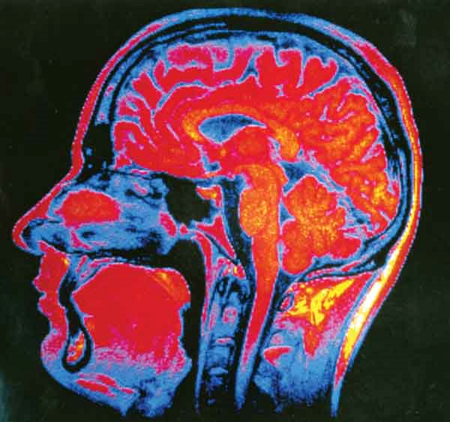
\includegraphics[width=1\textwidth,height=\textheight]{./pictures/brain_scan.png}}

}

\end{figure}

\hypertarget{hirnmasse}{%
\section{Hirnmasse}\label{hirnmasse}}

Das Gehirn eines Menschen ist vergleichsweise klein.

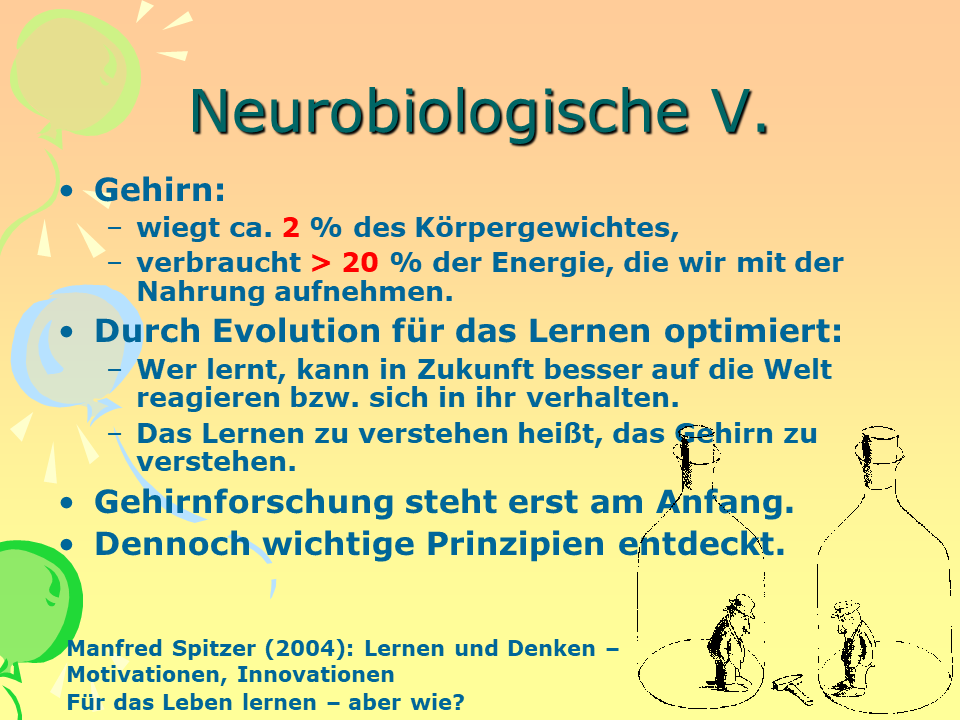
\includegraphics[width=1\textwidth,height=\textheight]{./pictures/neuro/Diapozitiv9.PNG}

Wie viel Hirnmasse hat der Mensch im Vergleich zu anderen Tieren?

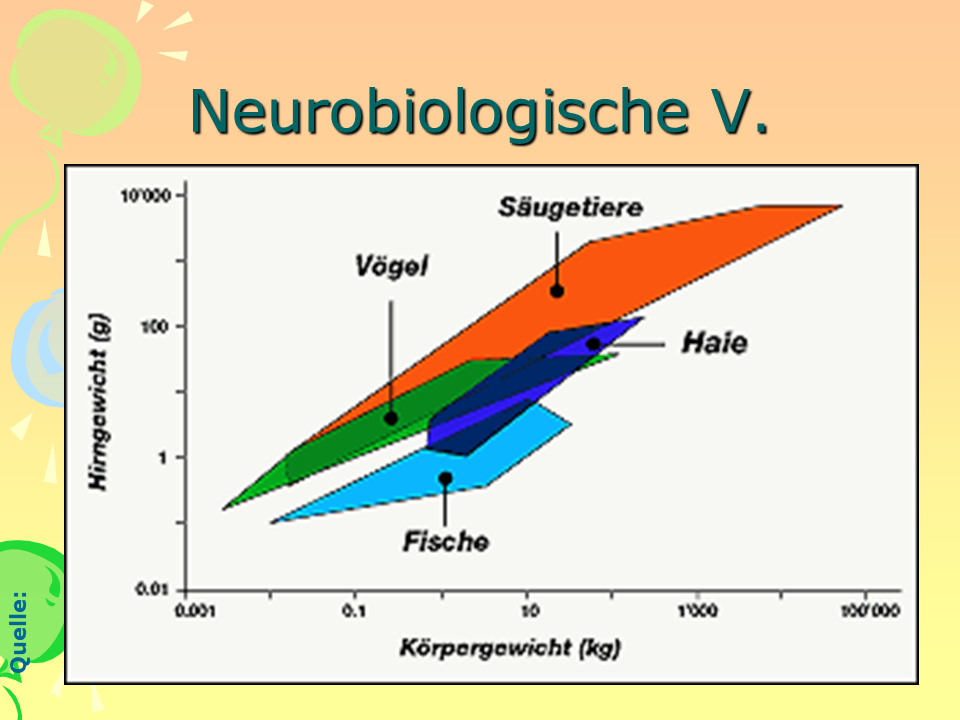
\includegraphics[width=1\textwidth,height=\textheight]{./pictures/neuro/Diapozitiv10.PNG}

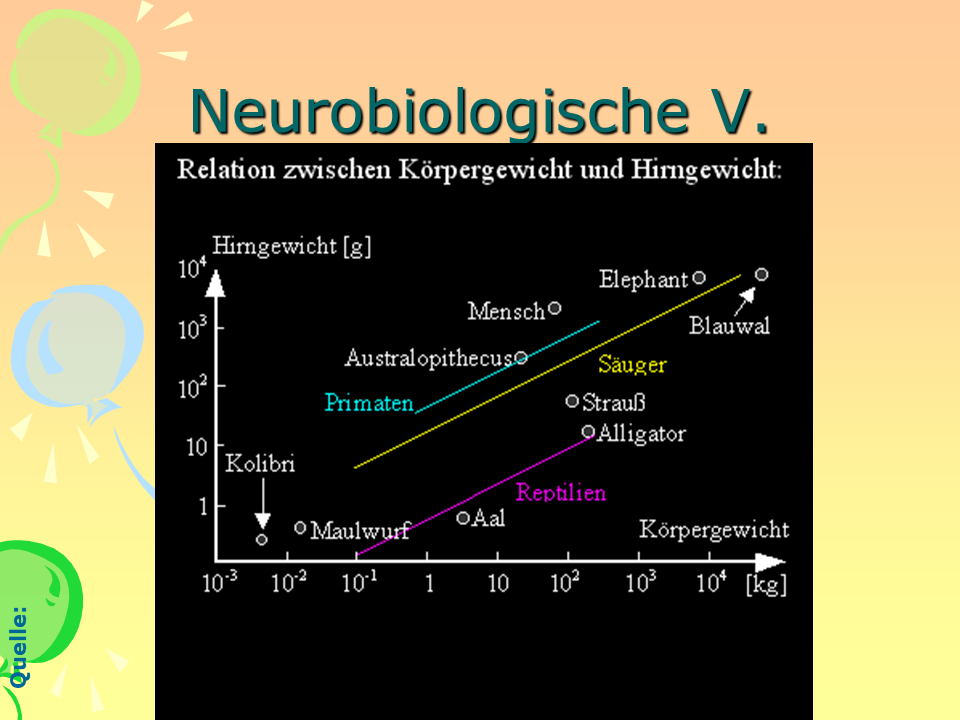
\includegraphics[width=1\textwidth,height=\textheight]{./pictures/neuro/Diapozitiv11.PNG}

\hypertarget{immer-online}{%
\section{Immer Online}\label{immer-online}}

Unser Gehirn ruht nie - ist immer ONLINE.

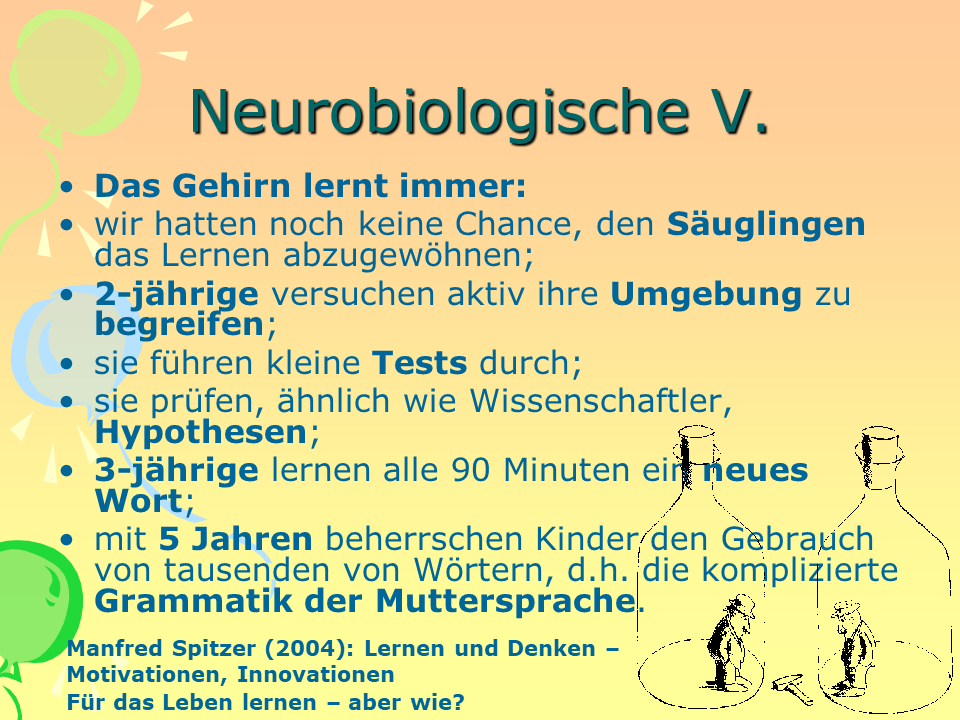
\includegraphics[width=1\textwidth,height=\textheight]{./pictures/neuro/Diapozitiv16.PNG}

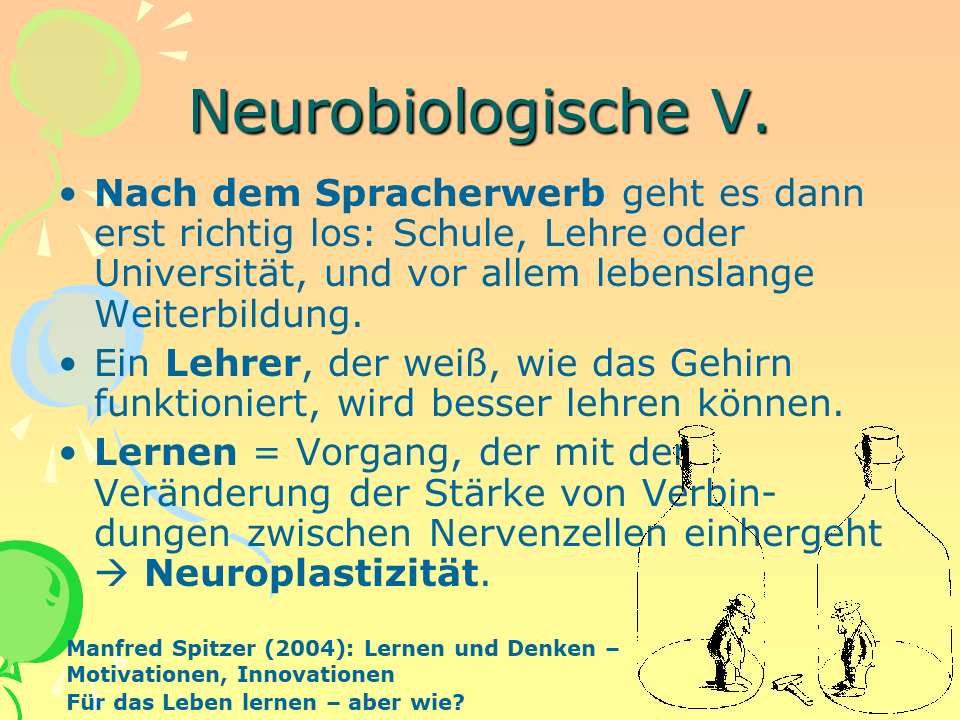
\includegraphics[width=1\textwidth,height=\textheight]{./pictures/neuro/Diapozitiv17.PNG}

\hypertarget{neuronale-netzwerke}{%
\section{Neuronale Netzwerke}\label{neuronale-netzwerke}}

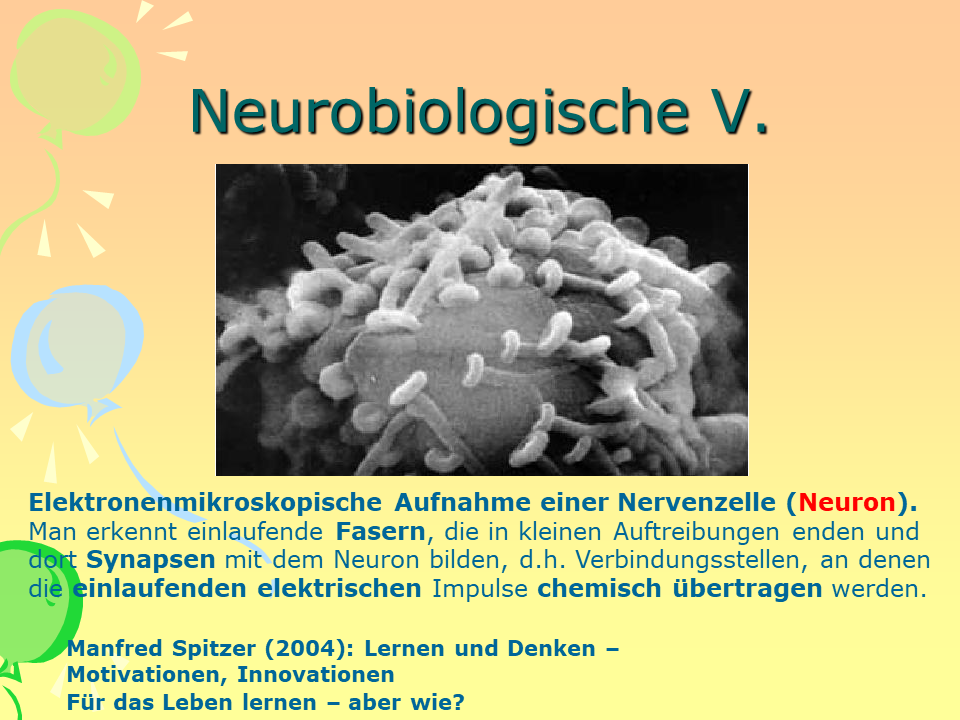
\includegraphics[width=1\textwidth,height=\textheight]{./pictures/neuro/Diapozitiv20.PNG}

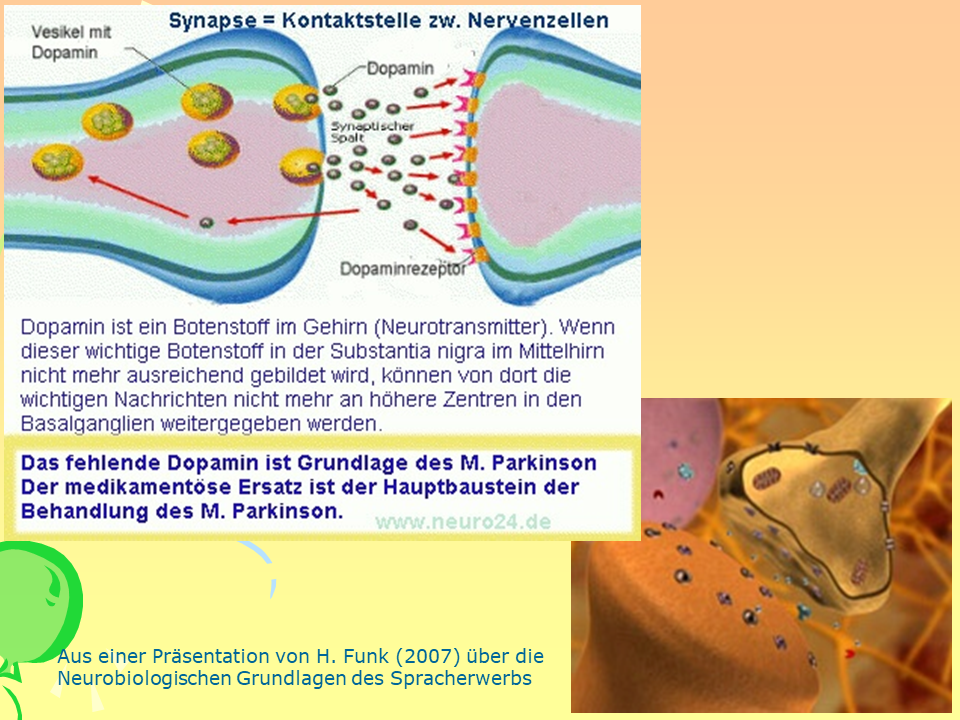
\includegraphics[width=1\textwidth,height=\textheight]{./pictures/neuro/Diapozitiv23.PNG}

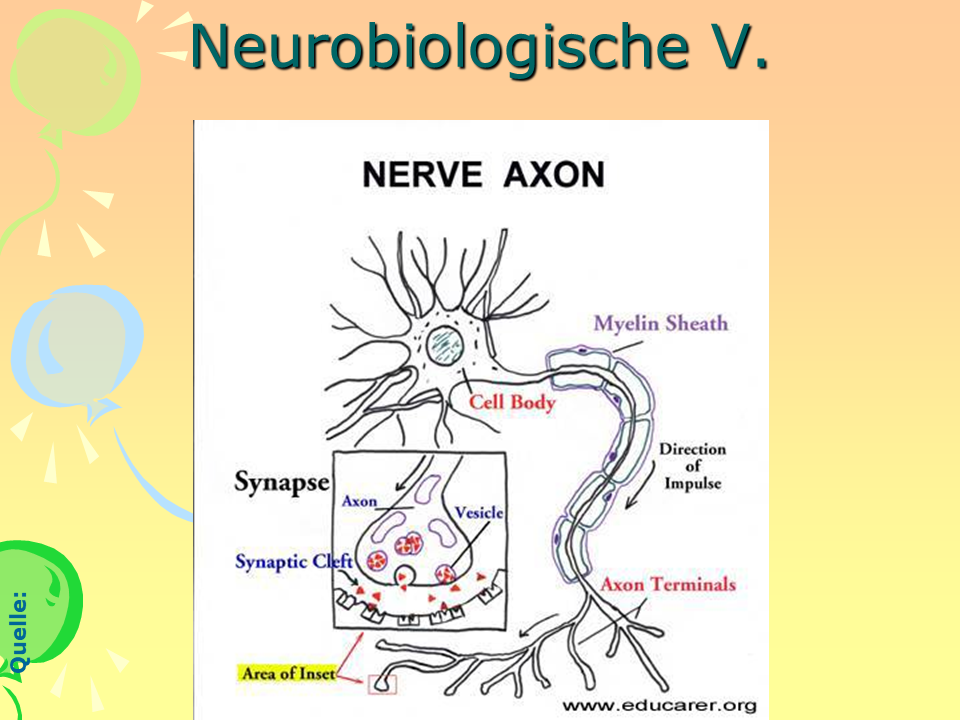
\includegraphics[width=1\textwidth,height=\textheight]{./pictures/neuro/Diapozitiv24.PNG}

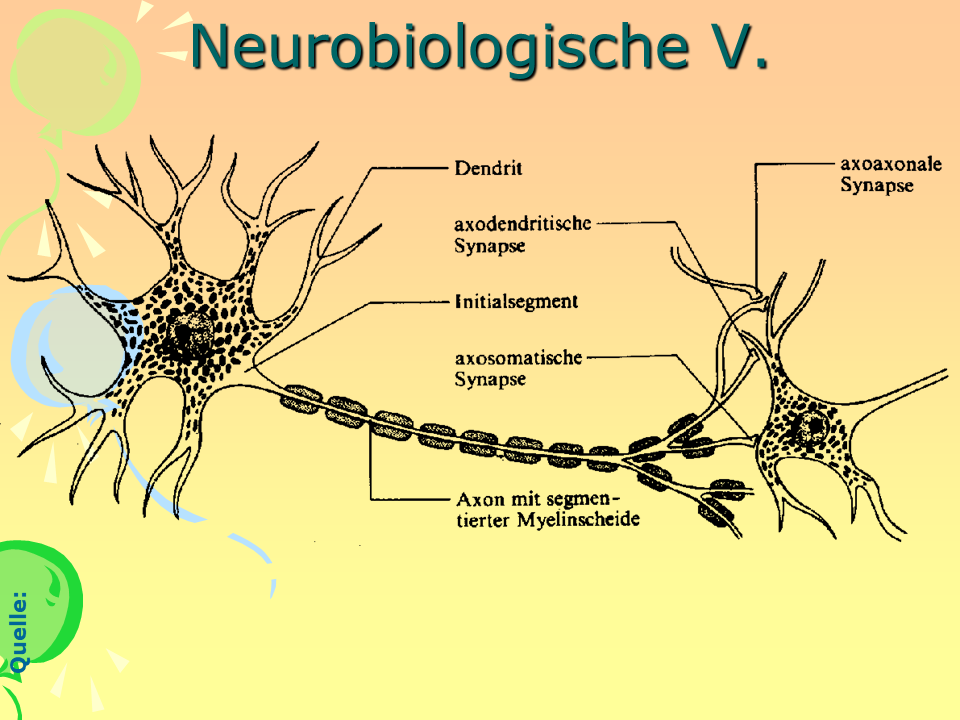
\includegraphics[width=1\textwidth,height=\textheight]{./pictures/neuro/Diapozitiv25.PNG}

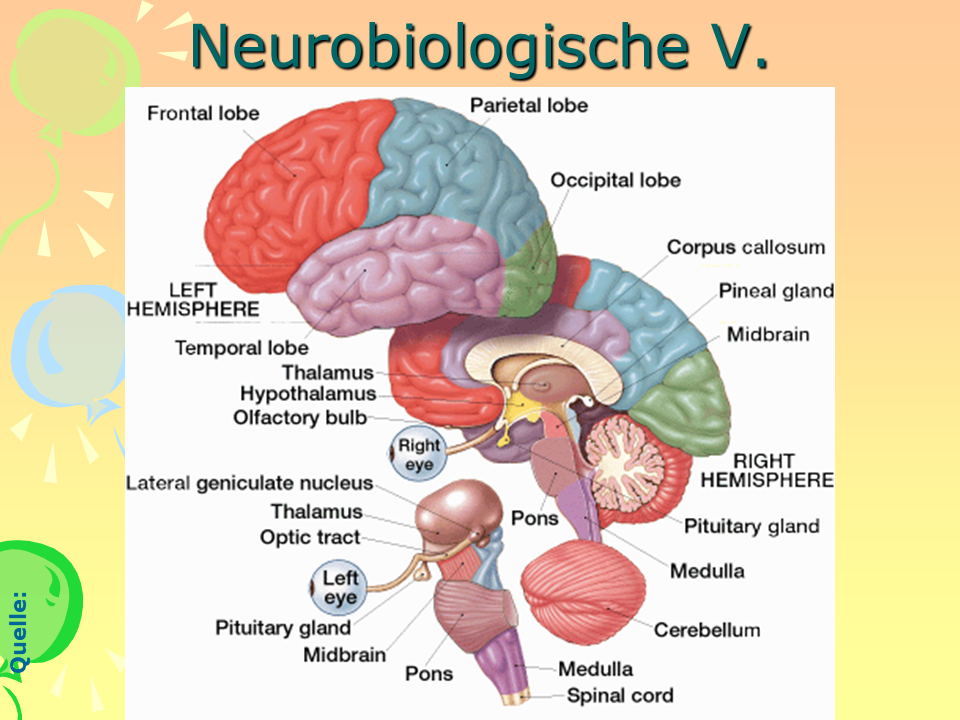
\includegraphics[width=1\textwidth,height=\textheight]{./pictures/neuro/Diapozitiv26.PNG}

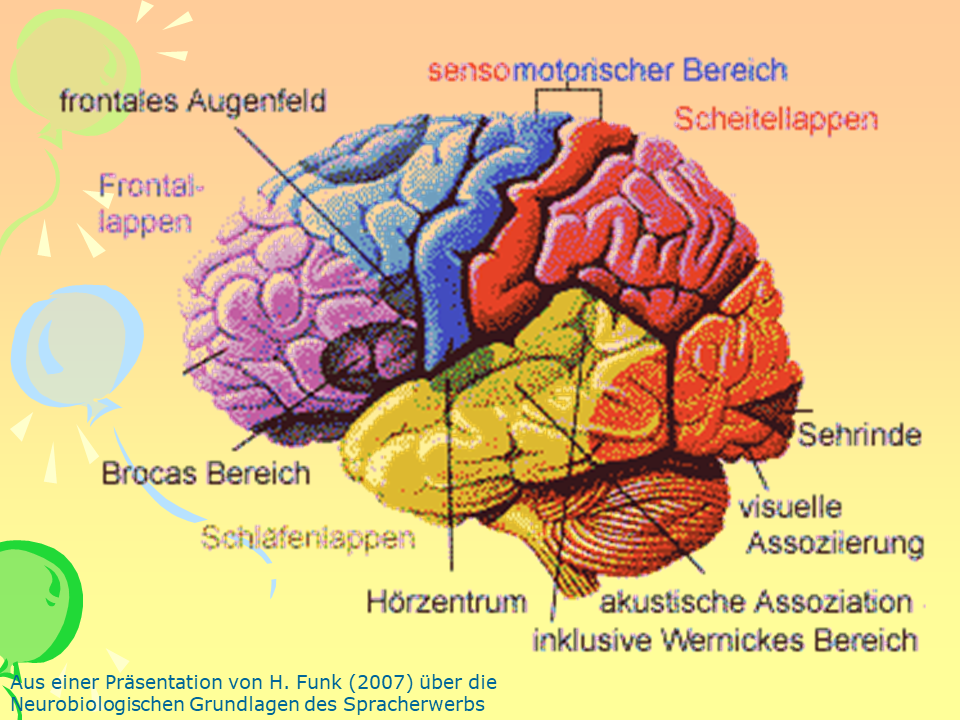
\includegraphics[width=1\textwidth,height=\textheight]{./pictures/neuro/Diapozitiv27.PNG}

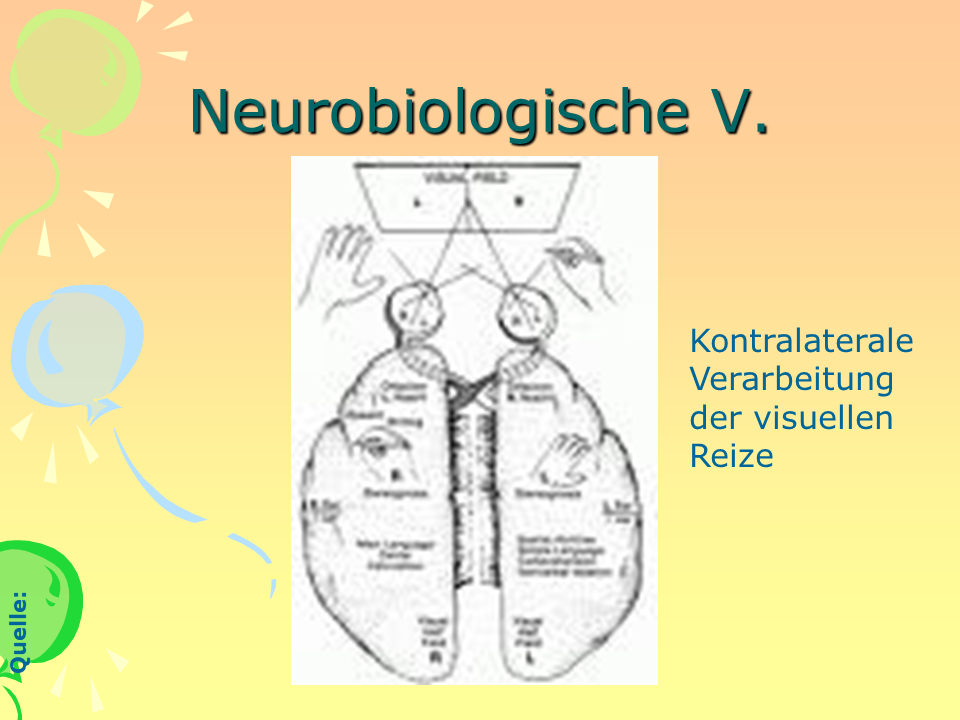
\includegraphics[width=1\textwidth,height=\textheight]{./pictures/neuro/Diapozitiv28.PNG}

\hypertarget{kortikale-landkarten}{%
\section{Kortikale Landkarten}\label{kortikale-landkarten}}

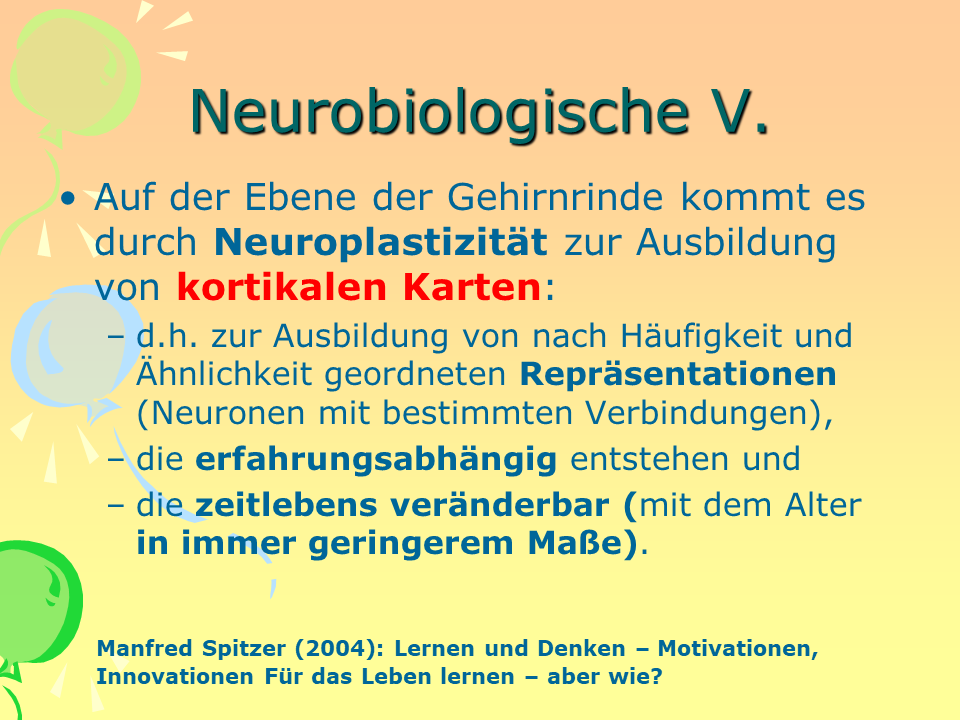
\includegraphics[width=1\textwidth,height=\textheight]{./pictures/neuro/Diapozitiv30.PNG}

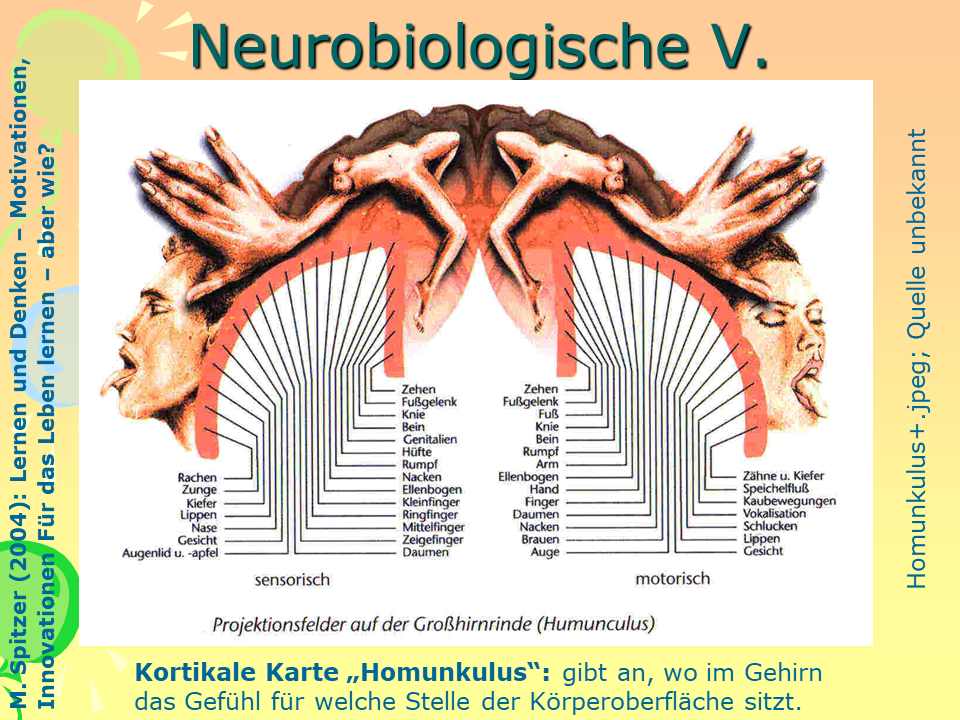
\includegraphics[width=1\textwidth,height=\textheight]{./pictures/neuro/Diapozitiv31.PNG}

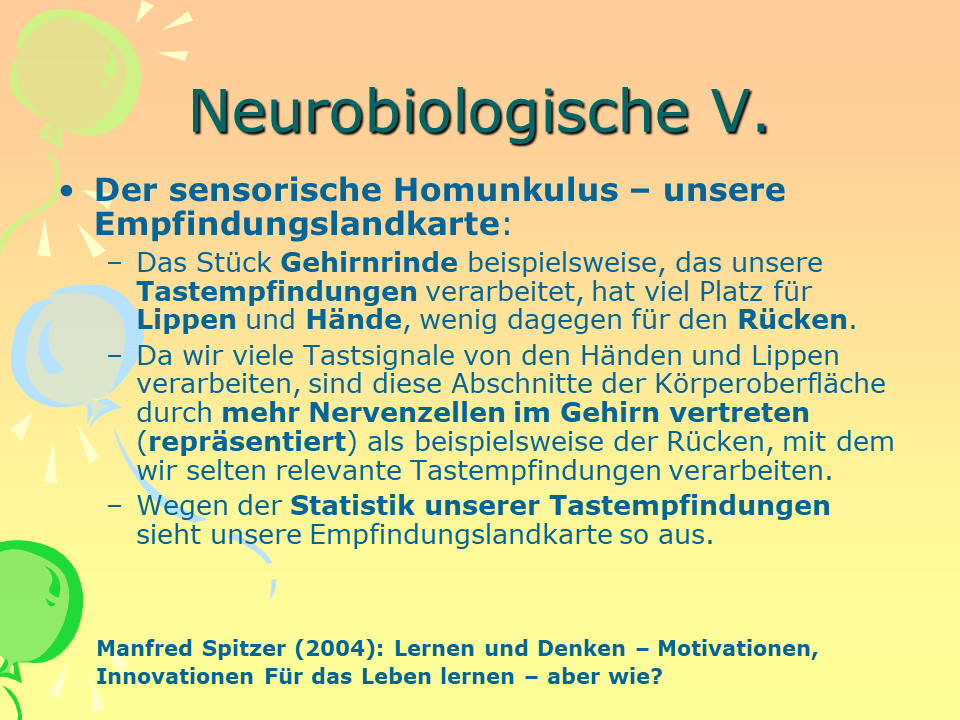
\includegraphics[width=1\textwidth,height=\textheight]{./pictures/neuro/Diapozitiv32.PNG}

\hypertarget{muster-und-intentionen}{%
\section{Muster und Intentionen}\label{muster-und-intentionen}}

Das Auge: Die rund 126 Mio. Zellen der Netzhaut liefern eine
unglaubliche Datenmenge ins Gehirn: pro Sekunde etwa 1,2 Megabyte. Das
entspricht einer Informationsmenge von 10.000 Seiten eines Buches.

Unser Gehirn versucht in den visuellen Reizen Muster zu erkennen, die an
bereits bekannte anknüpfen.

\textbf{Visuelle Muster}: Gestaltheorie - Figur vs.~Grund (Foregrounding
\& Backgrounding Processes)

\begin{figure}

{\centering 

\href{https://bildnerisches-gestalten.ch/index.php/wahrnehmung/}{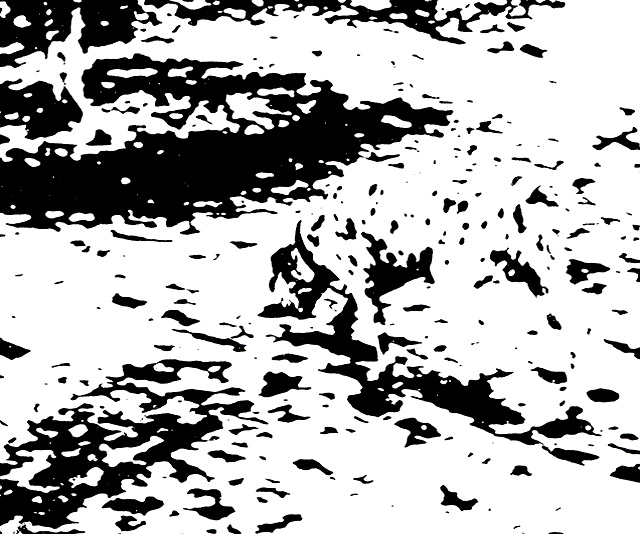
\includegraphics[width=1\textwidth,height=\textheight]{./pictures/dalmatiner.jpg}}

}

\end{figure}

Unser Gehirn versucht (holistische) Gestalten - Muster - zu erkennen,
wobei es sich auf Erfahrungswerte stützt und demnach zwischen
\textbf{Figur und Grund} unterscheidet (Vordergrund / Hintergrund). Die
Unterscheidung zwischen Figur und Grund fällt bei hohem Kontrast
leichter als bei geringem. Aus der anthropozentrischen Perspektive des
Menschen stellt stellt der Hund in dem Fleckenbild die Figur (den
Vordergrund) dar, die Umgebung dagegen den Hintergrund. Lebewesen werden
gewöhnlich als Figur interpretiert, da Lebewesen für Menschen
interessant bzw. besonders relevant sind und sich bewegen, während die
größere, statische Größe den Hintergrund bildet.

Akustische Reize (auch sprachliche) werden nach denselben Prinzipien
verarbeitet wie die visuellen Reize. In einem Satz, z.B. \emph{Der
Dalmatiner läuft durch den Wald,} wäre die Phrase \emph{der Dalmatiner}
dementsprechend die (wichtigere) Figur (der Vordergrund) und die Phrase
\emph{durch den Wald} der (weniger wichtige) Hintergrund der Aktion
(\emph{laufen}).

Zusammengestellt anhand von: - Stoll (2008)

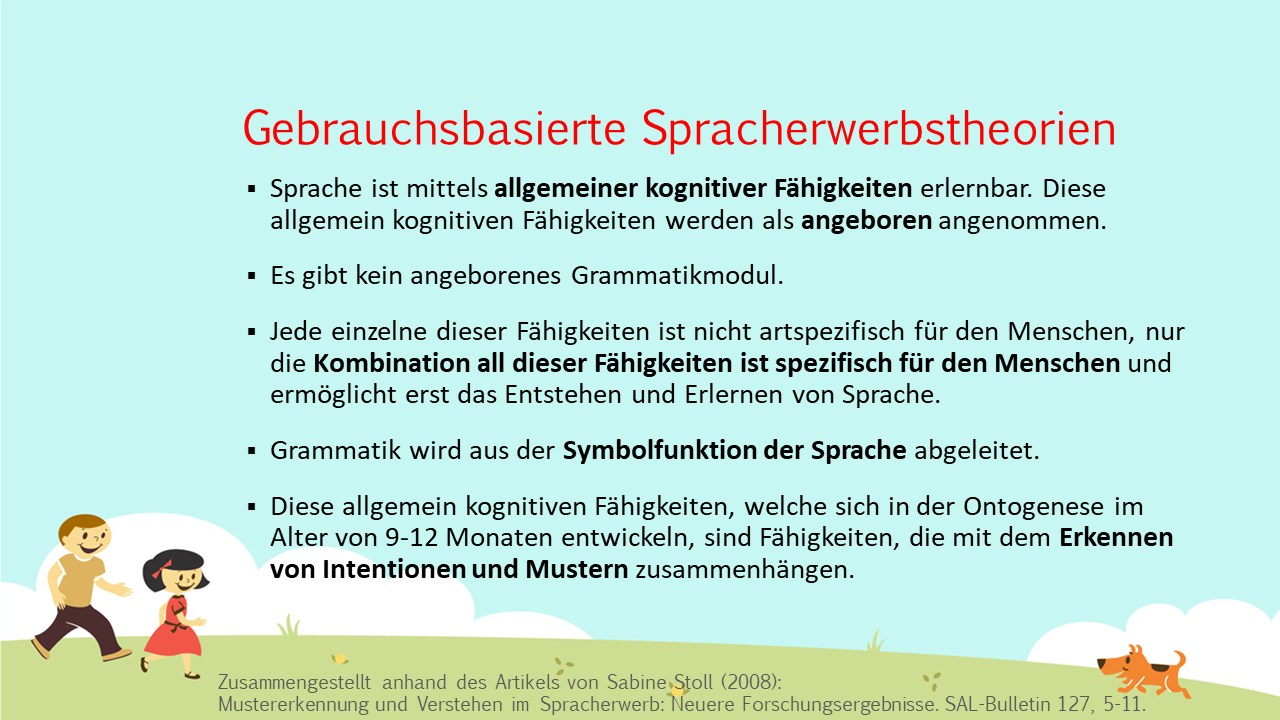
\includegraphics[width=1\textwidth,height=\textheight]{./pictures/muster_intentionen/Diapozitiv5.PNG}

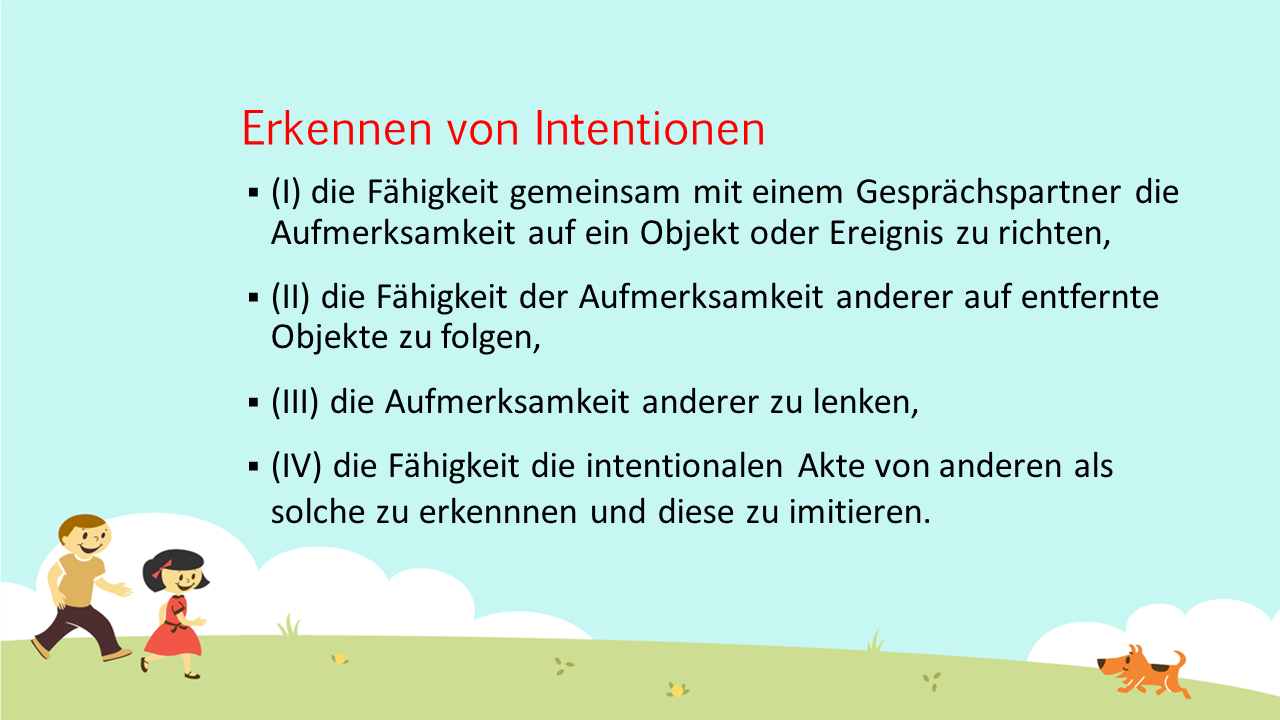
\includegraphics[width=1\textwidth,height=\textheight]{./pictures/muster_intentionen/Diapozitiv6.PNG}

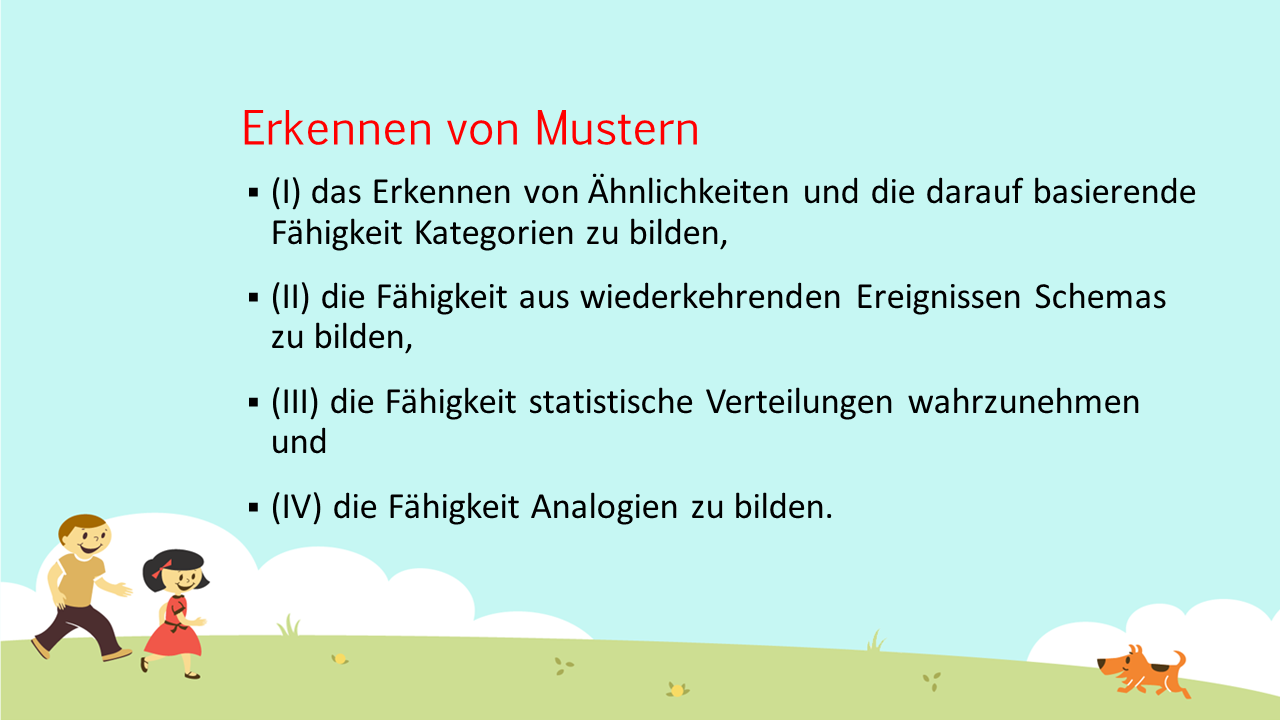
\includegraphics[width=1\textwidth,height=\textheight]{./pictures/muster_intentionen/Diapozitiv7.PNG}

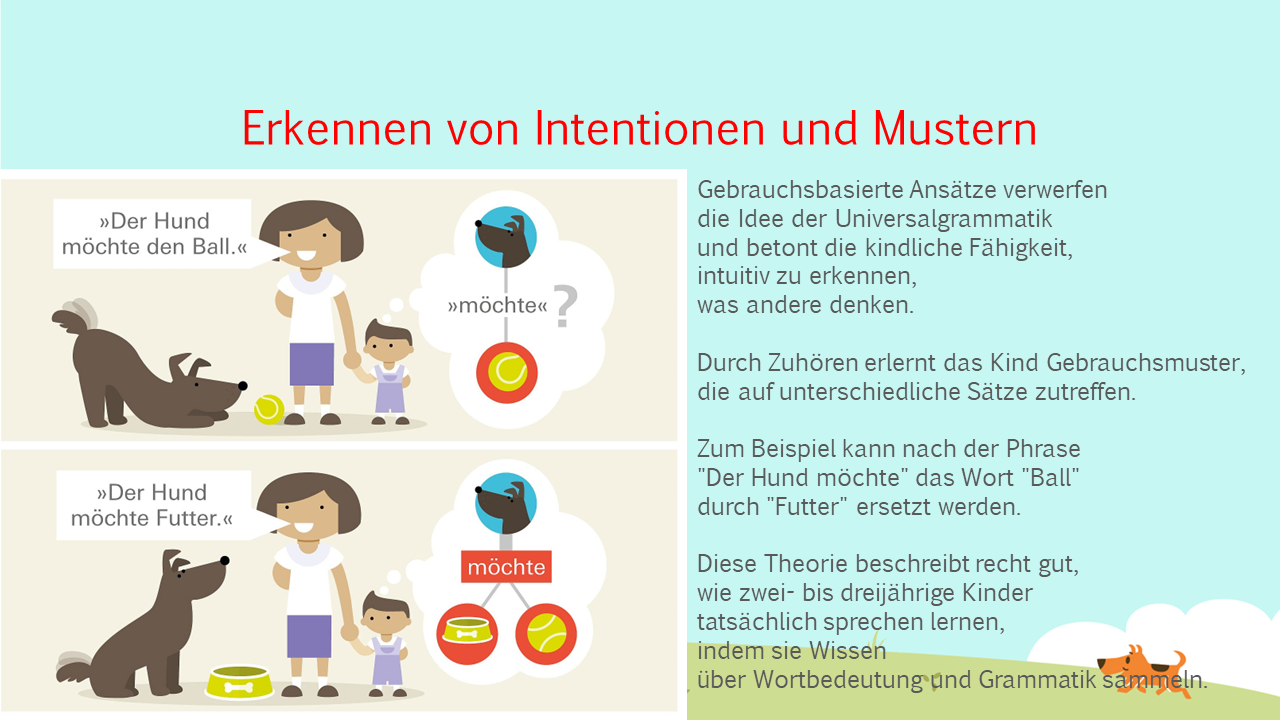
\includegraphics[width=1\textwidth,height=\textheight]{./pictures/muster_intentionen/Diapozitiv8.PNG}

\hypertarget{kategorienbildung}{%
\section{Kategorienbildung}\label{kategorienbildung}}

Beim Lernen bilden wir Kategorien, in die verschiedene Erscheinungen in
unserer Umwelt eingeordnet werden. Kategorien erleichtern Menschen den
Umgang mit ihrer Umwelt.

``\textbf{Kategorisierung} oder Kategorienbildung bezeichnet in der
Psychologie den Prozess, Objekte in Untergruppen oder Begriffsklassen
einzuteilen. (Stangl, 2023).''\\
\strut \\
Stangl, W. (2023, 13. März).
\href{https://lexikon.stangl.eu/7003/kategorisierung-kategorienbildung}{\emph{Kategorisierung
-- Kategorienbildung -- Online Lexikon für Psychologie \& Pädagogik}}.\\

\textbf{Kategorisierung} oder \textbf{kategoriales Denken} bezeichnet
die \href{https://de.wikipedia.org/wiki/Kognition}{kognitive} Fähigkeit,
unterschiedliche
\href{https://de.wikipedia.org/wiki/Entit\%C3\%A4t}{Entitäten}
(Gegenstände, Lebewesen, Vorgänge,
\href{https://de.wikipedia.org/wiki/Abstraktum}{Abstrakta})
\href{https://de.wikipedia.org/wiki/Intuition}{intuitiv} zu sortieren
und entsprechenden Sammelbegriffen (Kategorien) unterzuordnen. Diese
Kategorien basieren auf bestimmten Ähnlichkeiten oder auf dem Abgleich
mit dem theoretischen
Vor\href{https://de.wikipedia.org/wiki/Wissen}{wissen}. Die
Kategorienbildung ist ein fundamentaler Vorgang bei der Interpretation
und Bewertung von
\href{https://de.wikipedia.org/wiki/Wahrnehmung}{Wahrnehmungsinhalten},
dem Verständnis von Konzepten und
\href{https://de.wikipedia.org/wiki/Objekt_(Philosophie)}{Objekten}, bei
\href{https://de.wikipedia.org/wiki/Entscheidung}{Entscheidungsprozessen}
und bei allen Arten der Interaktion mit der
Umwelt.\textsuperscript{\href{https://de.wikipedia.org/wiki/Kategorisierung_(Kognitionswissenschaft)\#cite_note-Categorization-1}{{[}1{]}}}
Demzufolge sind Kategorien die „Grundbegriffe unseres
Denkens''.\textsuperscript{\href{https://de.wikipedia.org/wiki/Kategorisierung_(Kognitionswissenschaft)\#cite_note-Austeda-2}{{[}2{]}}}
{[}Kategorisierung{]}(https://de.wikipedia.org/wiki/Kategorisierung\_(Kognitionswissenschaft)

\begin{figure}

{\centering 

\href{https://www.keramikdeko.de/blog/alles-ueber-keramiktassen-und-keramikbecher-b74.html}{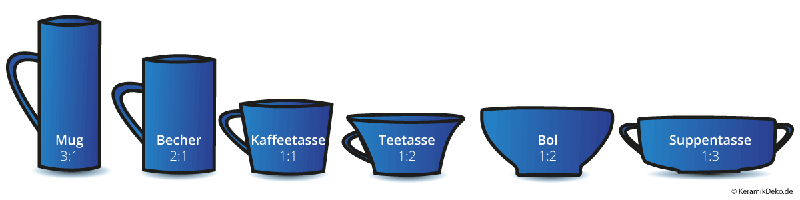
\includegraphics[width=1\textwidth,height=\textheight]{./pictures/Arten_von_Tassen_800.png}}

}

\end{figure}

\emph{Kategorielle Perzeption} von sprachlichen Stimuli: Die Suche nach
akustischen Hinweisen (engl. cues), die bei der Segmentierung größerer
Einheiten notwendig sind und die Aufdeckung von Kontrasten ermöglichen
(und damit Bedeutungsfindung). Gesucht wird nach distinktiven Merkmalen.
Akustische Signale sind (so wie visuelle Reize) höchstvariabel. Menschen
(bereits im Säuglingsalter) können sehr feine Unterschiede zwischen
akustischen Stimuli erkennen und sie für sprachliche Kategorisierung
nutzen.

\href{https://www.youtube.com/watch?v=8-fMLs-xCaA}{ListenLab} (Dauer:
15:00 Minuten):

\url{https://www.youtube.com/embed/8-fMLs-xCaA}

\href{https://www.youtube.com/watch?v=nNYhCP6NiUg}{ListenLab} (Dauer:
9:53 Minuten):

\url{https://www.youtube.com/embed/nNYhCP6NiUg}

\emph{Voice Onset Timing} im Englischen (vgl. mit Deutsch und
Slowenisch):\\
\href{https://www.youtube.com/watch?v=xR6FieNmWfg}{Isabel Cooke McKay}
(Dauer: 19:21 Minuten):

\url{https://www.youtube.com/embed/xR6FieNmWfg}

\href{https://www.youtube.com/watch?v=Kv6WBQVkHTo}{NPTEL IIT Guwahati}
(Dauer: 19:14 Minuten):

\url{https://www.youtube.com/embed/Kv6WBQVkHTo}

\hfill\break
Das Kleinkind ist schon früh in der Lage (vermutlich aufgrund seiner
genetischen Veranlagung) zwischen \textbf{sprachlichen und
nicht-sprachlichen Reizen} (Geräuschen) zu unterscheiden. Angeboren
scheint auch die \textbf{Denkfähigkeit}, also Begriffe zu entwickeln und
zu verarbeiten. Ebenfalls zur kognitiven Kapazität im weiteren Sinne
zählt die genetisch verankerte kognitive Anlage gehören (vermutlich
angeborene) \textbf{Mechanismen der Segmentierung} des sprachlichen
Schallstroms anhand bestimmter akustischer Eigenschaften, die Fähigkeit
zur \textbf{Kategorisierung} sprachlicher, etwa formal und/oder
funktional identischer Eigenschaften wahrscheinlich unter Anwendung
distributioneller Analyseverfahren, die Voraussetzung für die
Entwicklung von Strategien zur Analyse struktureller Eigenschaften von
Äußerungen aus den Morphemen und ihrer linearen Anordnung etc. Man wird
diesen Teil der kognitiven Ausstattung in der Literatur auch unter der
Bezeichnung \textbf{Angeborenes sprachliches Wissen} antreffen. Weniger
direkt als alle bisher erwähnten kognitiven Voraussetzungen, aber
vielleicht für die Sprachfähigkeit am ehesten eine Schlüsselfähigkeit
stellt das leistungsfähige \textbf{Gedächtnis} des Menschen dar. Eine
Schlüsselrolle kommt ihm insofern zu, als es die Begriffsbildung und die
komplizierten Analysevorgänge überhaupt erst möglich macht.\\

\hypertarget{sprachliches-wissen}{%
\section{Sprachliches Wissen}\label{sprachliches-wissen}}

``Viele Arten haben die Fähigkeit zweckmäßig und eindeutig zu
kommunizieren und jede verwendet dazu ein je artspezifisches System. Die
Kommunikationsverfahren sind bestimmt von biologischen, sozialen und
kognitiven Voraussetzungen der jeweiligen Art und ihrer Lebenswelt. Und
die artspezifischen Sprachen sind es auch -- aber anders; Hauser (1996).
Die Kommunikationsverfahren sind angepasst einerseits an die peripheren
Organe der Produktion und Rezeption, andererseits an die psychischen
Repräsentationen der jeweiligen Organismen.'' - Dietrich (2002)

``Das \textbf{sprachliche Wissen} stellt dem Menschen die Mittel für die
sprachliche Kommunikation über nicht-sprachliche psychische Dinge
bereit, und die Organisation dieses Wissensbestandes prägt alle
Modalitäten der sprachlichen Verständigung.'' - Dietrich (2002)

Zum sprachlichen Wissen gehören Kenntnisse der Inhalts- und der
Ausdrucksseite:

\begin{itemize}
\item
  semantische Kenntnisse (Konzepte),
\item
  das Erkennen und die Unterscheidung von Äußerungsabsichten,
\item
  die Kenntnis der Worteigenschaften (syntaktische, morphologische,
  phonologische, graphematische Eigenschaften von Wörtern und ihren
  Verbindungen zu größeren Einheiten),
\item
  Textmusterwissen.
\end{itemize}

\hypertarget{das-mentale-lexikon}{%
\subsection{Das mentale Lexikon}\label{das-mentale-lexikon}}

Mit dem \textbf{mentalen Lexikon} meint man das sprachliche Wissen im
Langzeitgedächtnis.

Sind sprachliche Einheiten (Informationsbündel - chunks) wirklich als
\textbf{Einheiten} im \textbf{Langzeitgedächtnis} gespeichert? Wenn das
der Fall ist, so müssten sie auch als Einheit verarbeitet werden, also
anders als die im Informationsbündel enthaltenen Bestandteile. -
Dietrich (2002)

Wird eine so grundlegende sprachliche Einheit wie das \textbf{Wort als
Einheit} in unserem Langzeitgedächtnis gespeichert?

\textbf{Worthaftigkeitseffekt} (Wortüberlegenheitseffekt - Word
Superiority Effect):

Die Sprachrezeption erlaubt eher einen kontrollierten Zugang zu den
Verarbeitungsprozessen im Gehirn als die Sprachproduktion. Insbesondere
das Lesen ist relativ leicht zu kontrollieren und zu beobachten. Das
Lesen beginnt mit der visuellen Wahrnehmung der Buchstaben. Diese müssen
kurzfristig in einem begrenzten Speicher aufgenommen werden. Dies nimmt
Zeit in Anspruch. Eine einfache Annahme ist, das Lesen eines Buchstaben
schneller geht als das Lesen von zwei oder mehreren. Aber man hat
beobachtet, dass in manchen Fällen die Verarbeitung eines Buchstaben
länger dauern kann als die von zwei oder mehreren. Dies hat man vor
allem bei Buchstabenfolgen bemerkt, die kurze Wörter darstellen. Handelt
es sich nun um einen allgemeinen Worthaftigkeitseffekt oder nur um eine
Eigenschaft spezieller Wörter?

Bei der Überprüfung zeigt sich zunächst, dass die Lesegeschwindigkeit
für Buchstabenfolgen, die Wörter bilden, kürzer ist als für Nichtwörter.
Dies kann mit der \textbf{Worthaftigkeit} erklärt werden \textbf{oder}
auch mit der \textbf{Wahrscheinlichkeit} der Abfolge von Buchstaben in
einer Sprache. Im letzteren Fall würde es sich um einen
\textbf{Häufigkeitseffekt} auf Buchstabenebene handeln und nicht um
einen Worthaftigkeitseffekt.

\textbf{Experiment zum Nachweis des Wortüberlegenheitseffekts} (Reicher
1969):

In schneller Folge und sehr kurz werden eine Buchstabenfolge, MAUS (=
Wortbedingung) oder AMUS (Non-Wort-Bedingung) und sodann eine
entsprechende maskierte Buchstabenfolge, z.B. MAU bzw. AMU gezeigt.

Welcher Buchstabe an der maskierten Position stand, kann nach sehr
kurzer Lesezeit (\textless= 100 ms) nicht aus der Erinnerung abgerufen
werden.

Dann folgt die Aufgabe: Es wird der Buchstabe S oder L gezeigt und die
Entscheidung verlangt, ob es der letzte Buchstabe der zuerst gesehenen
Folge, also MAUS bzw. AMUS war.

\textbf{Ergebnis}: Die Entscheidung ist unter Wort-Bedingung signifikant
häufiger korrekt als unter Nicht-Wort-Bedingung, und zwar obwohl beide
Buchstaben (S und L) auf den Buchstaben ``a'' gleich häufig folgen und
zu einem Wort ergänzen. Bei Wahrnehmung eines Wortes wird das
lexikalische Wissen abgerufen. Dadurch wird das Lesen von Wörtern
beschleunigt.\\

Versuchspersonen lasen Buchstabenfolgen (\textbf{Wörter}, Non-Wörter und
sog. Pseudo-Wörter), die jeweils sehr kurz visuell präsentiert wurden
(Ripamonti et al.~(2014)). Sie lasen die Buchstabenfolgen einmal mit dem
linken Auge (kontralaterale Verarbeitung über die rechte Gehirnhälfte),
einmal mit dem rechten (kontralaterale linkshemisphärische
Verarbeitung).

Ein \textbf{Pseudo-Wort} ist eine Buchstabenfolge, die nach den
phonotaktischen Regeln in der jeweiligen Sprache ein Wort darstellen
könnte, aber keine Bedeutung hat und nicht im mentalen Lexikon enthalten
ist. Ein \textbf{Nicht-Wort} ist eines, das ebenfalls ohne Bedeutung und
nicht im mentalen Lexikon vorhanden ist und dessen Buchstabenfolge nicht
den phonotaktischen Regeln folgt.

Im Deutschen ist z. B.

\begin{itemize}
\item
  h-a-u-s ein Wort,
\item
  h-a-u-m ein Pseudowort und
\item
  h-s-u-a ein Nicht-Wort.
\end{itemize}

\textbf{Ergebnis}: An Nicht-Wörter erinnerten sich die Versuchspersonen
schlechter als an Wörter und Pseudowörter. Zwischen Wörtern und
Pseudowörtern (des Italienischen) fand man keinen wesentlichen
Unterschied.

\textbf{Schlussfolgerung}: Beim Lesen sind \textbf{prälexikalische}
Prozesse beteiligt (d.h. ein Zugriff auf das mentale Lexikon ist nicht
notwendig). Dies wird dadurch bestätigt, dass es zwischen linkem und
rechtem Auge keinen wesentlichen Unterschied gab (also Prozesse über die
linke als auch über die rechte Gehirnhälfte ablaufen können).

\textbf{Stroop-Effekt}: Dieser Effekt bestätigt ebenfalls den
Worthaftigkeitseffekt, denn Buchstabenfolgen, die ein Wort ergeben,
werden automatisch als Wort verarbeitet. Die Verarbeitung ist so stark
automatisiert, dass man die Verarbeitung kaum unterdrücken kann.

Mit der Bezeichnung \emph{Stroop-Effekt} bezieht man sich auf mehrere
Reaktionsmuster bei Aufgaben:

\begin{enumerate}
\def\labelenumi{\arabic{enumi}.}
\item
  die Farbe einer Fläche zu nennen,
\item
  eine Farbbezeichnung zu lesen, die mit der Schriftfarbe kongruiert
  (übereinstimmt),
\item
  eine Farbbezeichnung zu lesen, die mit der Schriftfarbe nicht
  kongruiert (kontrastiert),
\item
  die Schriftfarbe einer nicht-kongruenten Farbbezeichnung zu nennen.
\end{enumerate}

Der Vergleich der Bedingungen 2 und 3 zeigt den (geringen) Effekt der
Farbe auf das Lesen eines Wortes, der Vergleich von 1 und 4 den
Interferenzeffekt, der durch die Bedeutung des Farbwortes ausgelöst wird
und die Benennung der Farbe beeinträchtigt.

Verglichen werden die Lesezeiten unter den vier verschiedenen
Bedingungen.

Zwischen Wortbedeutung und Farbvorstellung gibt es demnach einen
Interferenzeffekt. Die sprachliche Einheit des Wortes zwingt das Denken,
sich mit seiner Verarbeitung zu beschäftigen und beeinträchtigt die
Verarbeitung der Farbwahrnehmung. - Dietrich (2002)

Es gibt zahlreiche Versionen des Stroop-Experiments, der
Interferenzeffekte aufdeckt. --\textgreater{} Pinkers Vortrag bei Google
(YouTube).

Dietrich (2002): Bearbeiten !!!!

\textbf{Lauterkennung im Wortkontext} und Phonemrestauration: Auch die
Verarbeitung von Lauten wird davon beeinflusst, ob der Laut als
Bestandteil eines Wortes gehört wird oder nicht. Unter anderem wird die
Fähigkeit davon beeinflusst, Urteile über auditiv Wahrgenommenes zu
fällen. Wird in einem gehörten Wort ein Laut einmal mit Geräusch
überlagert, ein andermal durch Geräusch vollständig ersetzt, so wird
letzteres schlechter erkannt. Dieser Effekt tritt nicht auf beim Hören
gleichartig unterschiedener Nicht-Wort-Paare (vgl. Samuel 1986).

Der Effekt der sog. \textbf{Phonemrestauration} (phonemic restoration
effect) liefert Evidenz für dieselbe Annahme (vgl. Warren 1970;
Sivonen/Maess/ Lattner/Friederici 2006; Kashino 2006). Wird ein Laut
eines Wortes vollständig von einem nicht-sprachlichen Laut überlagert,
fällt dies Hörern bei der Wahrnehmung nicht notwendigerweise auf.
Versuchspersonen geben sogar an, den Laut deutlich gehört zu haben. Je
nach Kontext, ersetzen Hörer einen fehlenden Laut sogar in verschiedener
Weise (s. Kapitel 5 für eine detaillierte Erläuterung)\\

\textbf{Wortfrequenz}: Auch der Frequenzeffekt stützt die Annahme von
der kognitiven Realität des Wortes. Ein Wort, das in der täglichen
Kommunikation zwischen Mitgliedern der Sprachgemeinschaft häufig
verwendet wird, wird vom Einzelnen schneller verarbeitet. Die Frequenz
ist also eine Eigenschaft des Wortes und sie lässt sich nicht aus der
Frequenz seiner Laute ableiten. Der Frequenzeffekt zählt mit zu den
stabilsten Phänomenen lexikalischer Verarbeitung (vgl. Jescheniak/Levelt
1994; Jescheniak 2002; Graf/ Nagler/Jacobs 2005; jedoch auch
Jescheniak/Meyer/Levelt 2003b).\\

\hfill\break

\hypertarget{sprachareale}{%
\section{Sprachareale}\label{sprachareale}}

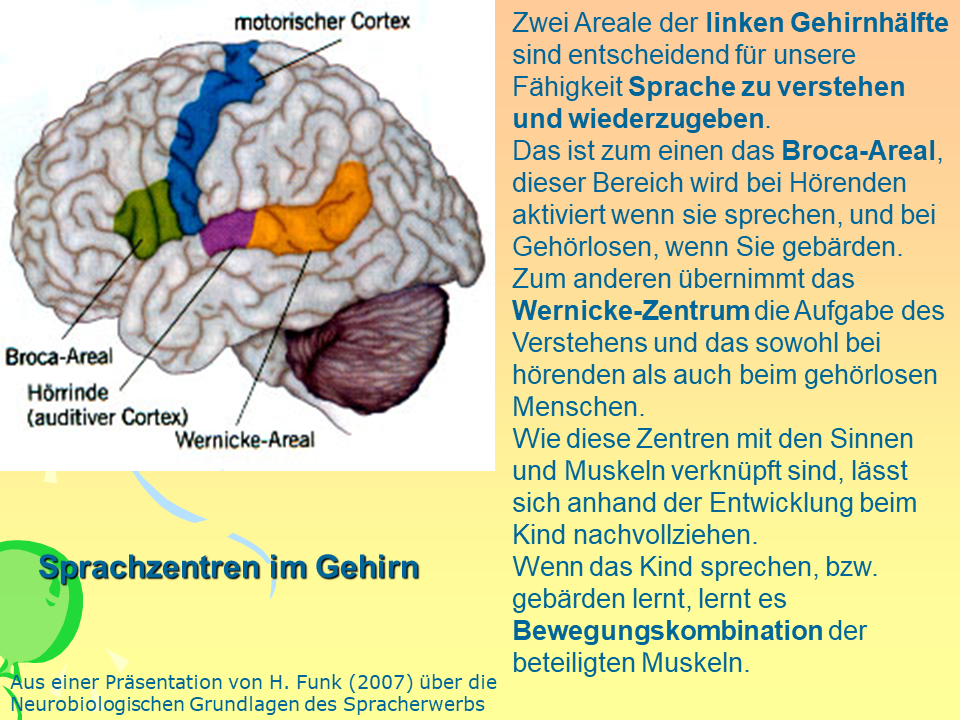
\includegraphics[width=1\textwidth,height=\textheight]{./pictures/neuro/Diapozitiv35.PNG}

\hypertarget{geduxe4chtnissysteme}{%
\section{Gedächtnissysteme}\label{geduxe4chtnissysteme}}

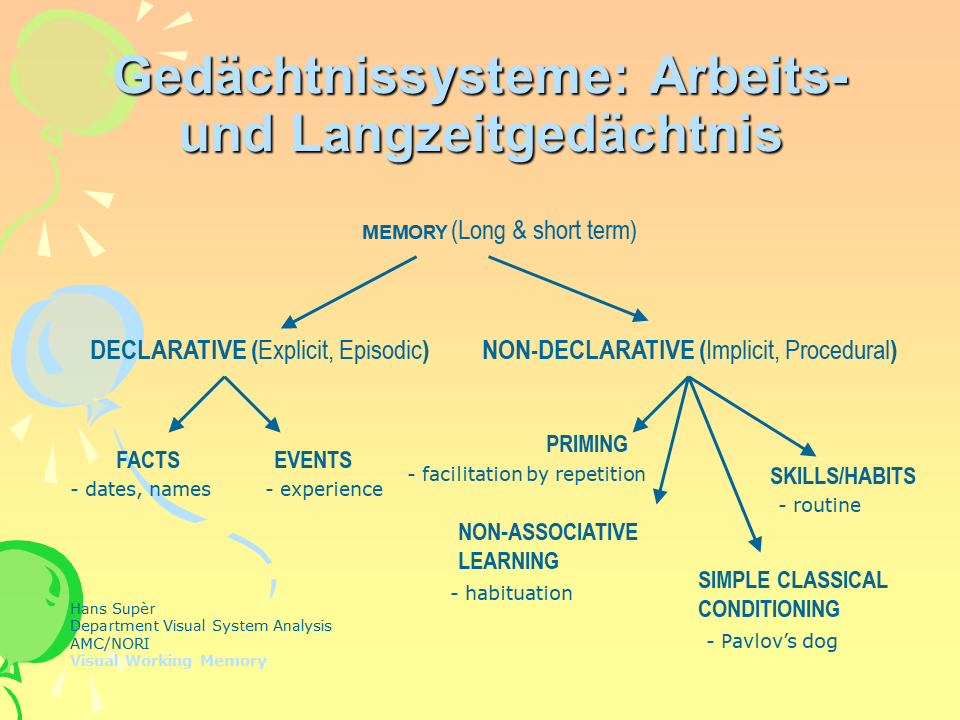
\includegraphics[width=1\textwidth,height=\textheight]{./pictures/neuro/Diapozitiv37.PNG}

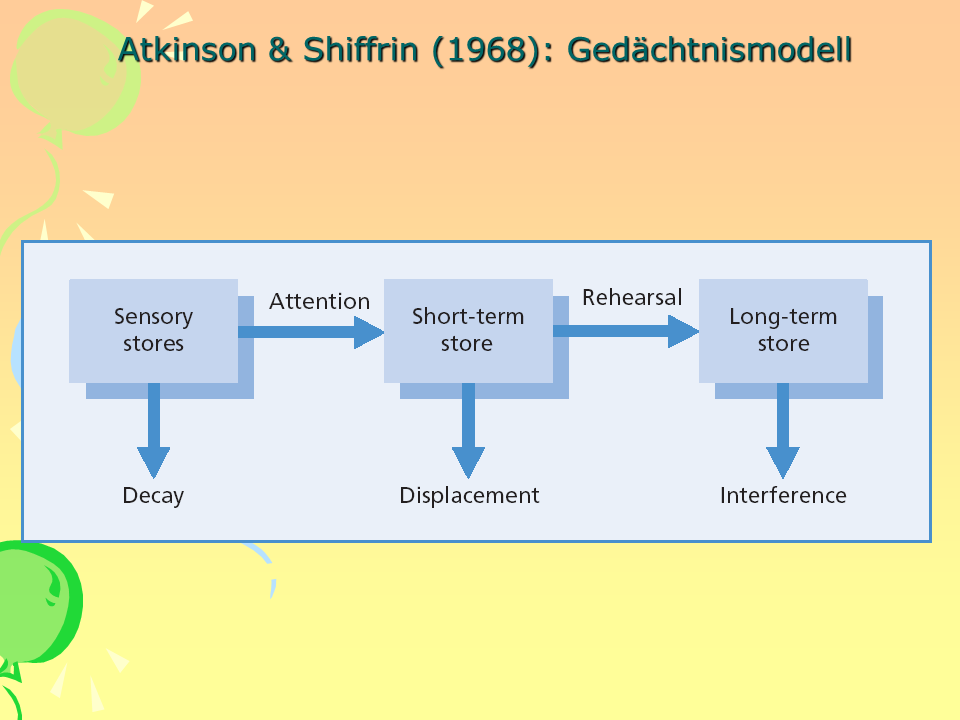
\includegraphics[width=1\textwidth,height=\textheight]{./pictures/neuro/Diapozitiv38.PNG}

\hypertarget{sensorisches-geduxe4chtnis}{%
\subsection{Sensorisches Gedächtnis}\label{sensorisches-geduxe4chtnis}}

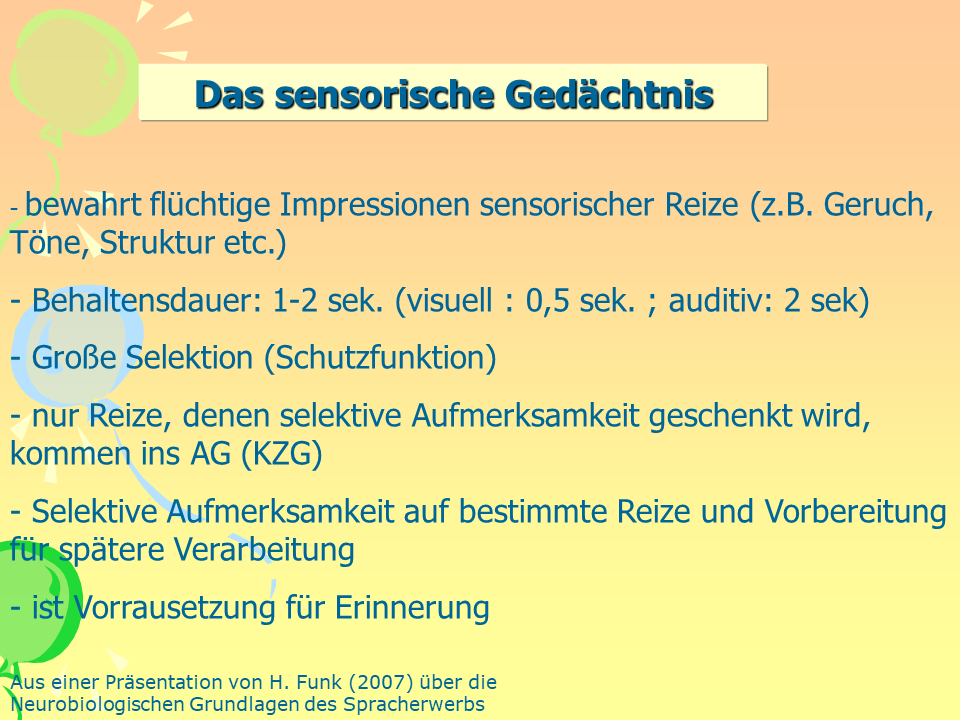
\includegraphics[width=1\textwidth,height=\textheight]{./pictures/neuro/Diapozitiv39.PNG}

\hypertarget{arbeitsgeduxe4chtnis}{%
\subsection{Arbeitsgedächtnis}\label{arbeitsgeduxe4chtnis}}

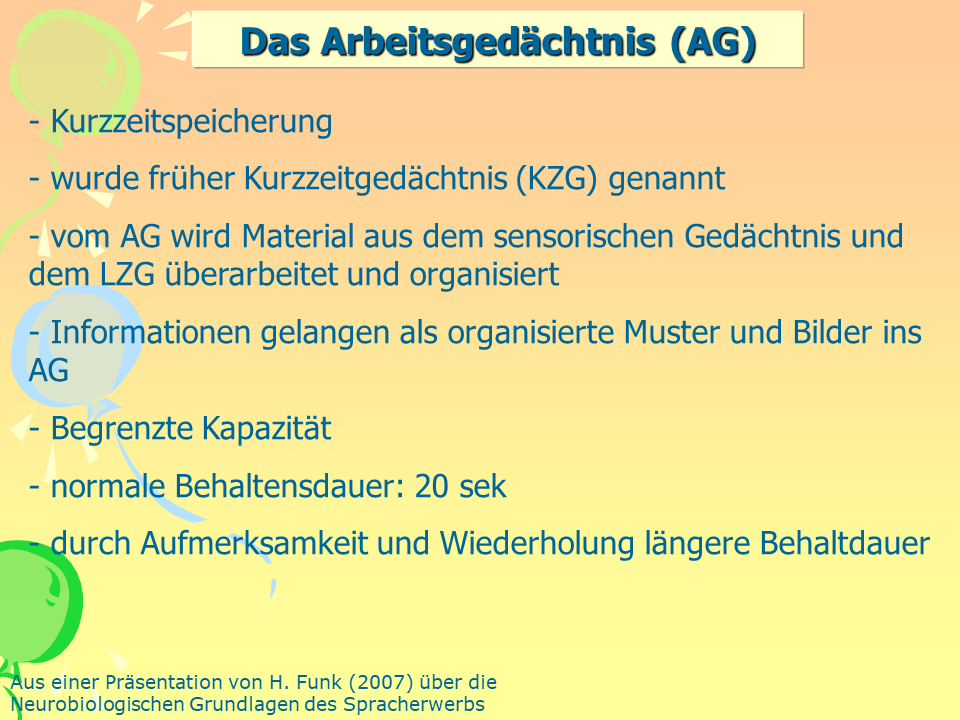
\includegraphics[width=1\textwidth,height=\textheight]{./pictures/neuro/Diapozitiv40.PNG}

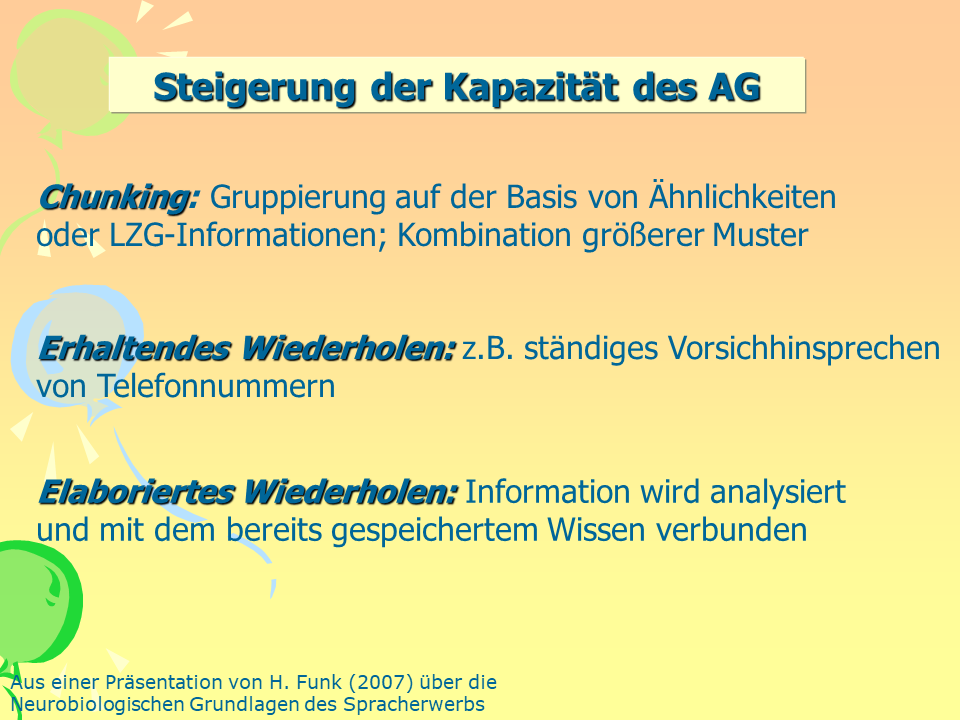
\includegraphics[width=1\textwidth,height=\textheight]{./pictures/neuro/Diapozitiv41.PNG}

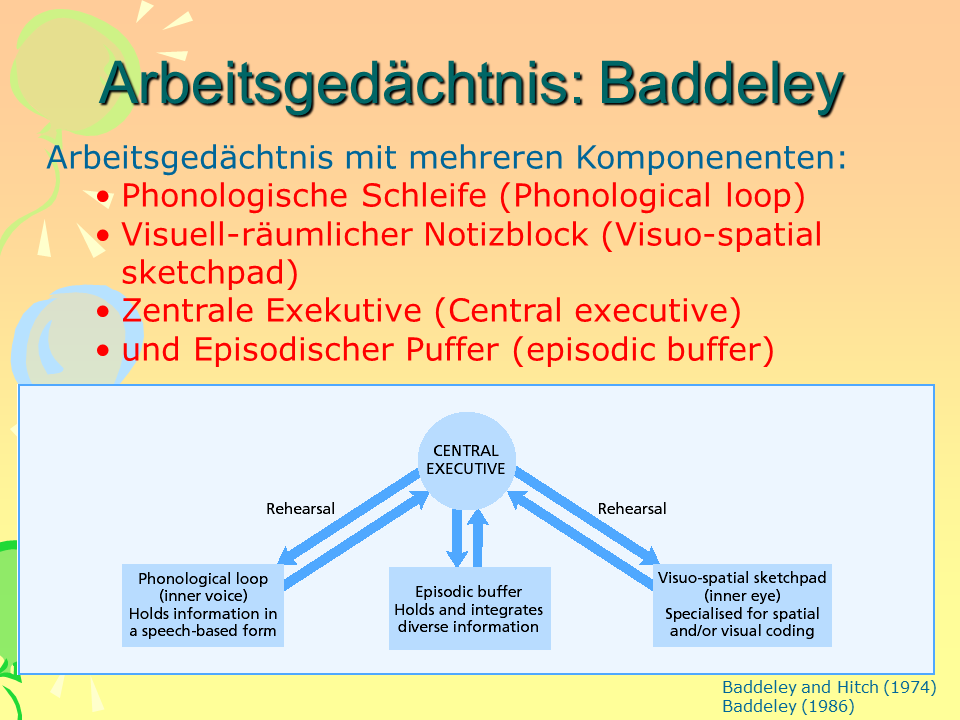
\includegraphics[width=1\textwidth,height=\textheight]{./pictures/neuro/Diapozitiv42.PNG}

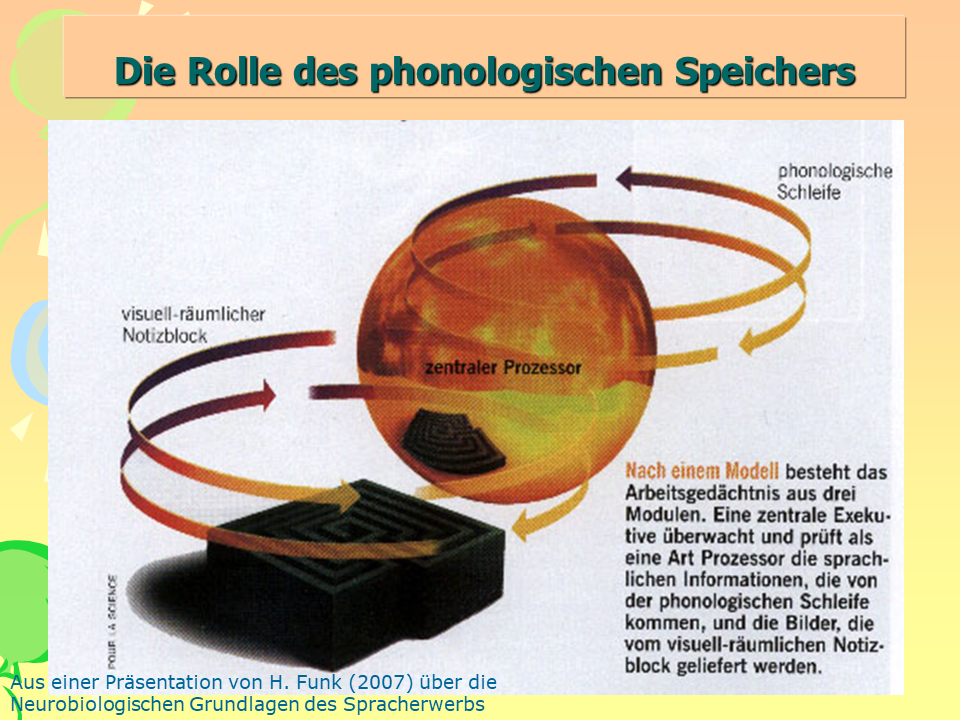
\includegraphics[width=1\textwidth,height=\textheight]{./pictures/neuro/Diapozitiv43.PNG}

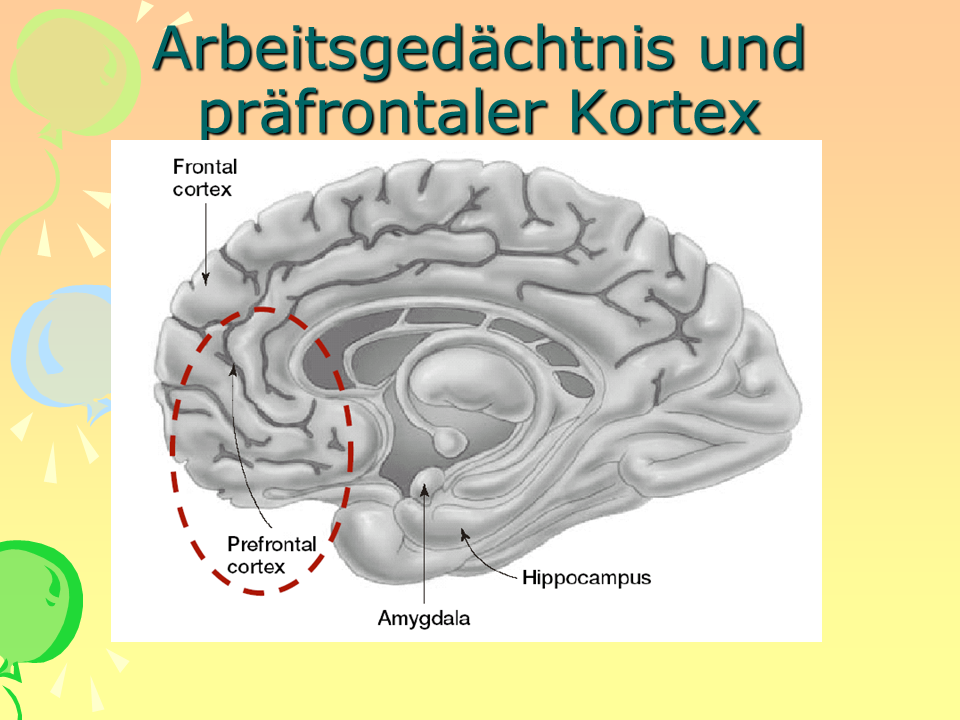
\includegraphics[width=1\textwidth,height=\textheight]{./pictures/neuro/Diapozitiv44.PNG}

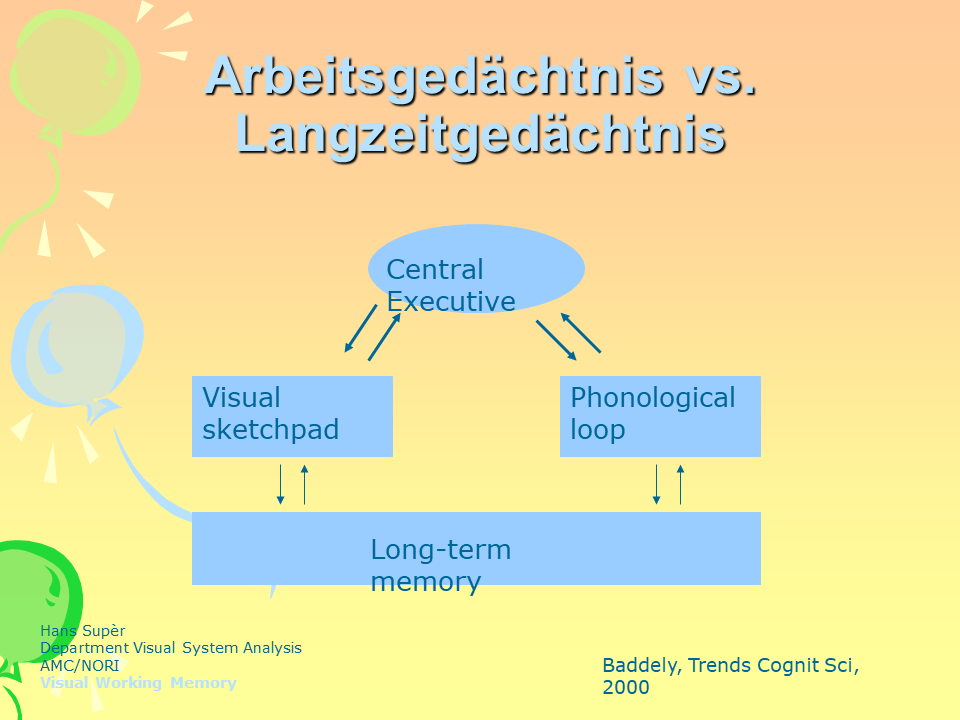
\includegraphics[width=1\textwidth,height=\textheight]{./pictures/neuro/Diapozitiv45.PNG}

\hypertarget{langzeitgeduxe4chtnis}{%
\subsection{Langzeitgedächtnis}\label{langzeitgeduxe4chtnis}}

\hypertarget{regeln}{%
\subsubsection{Regeln}\label{regeln}}

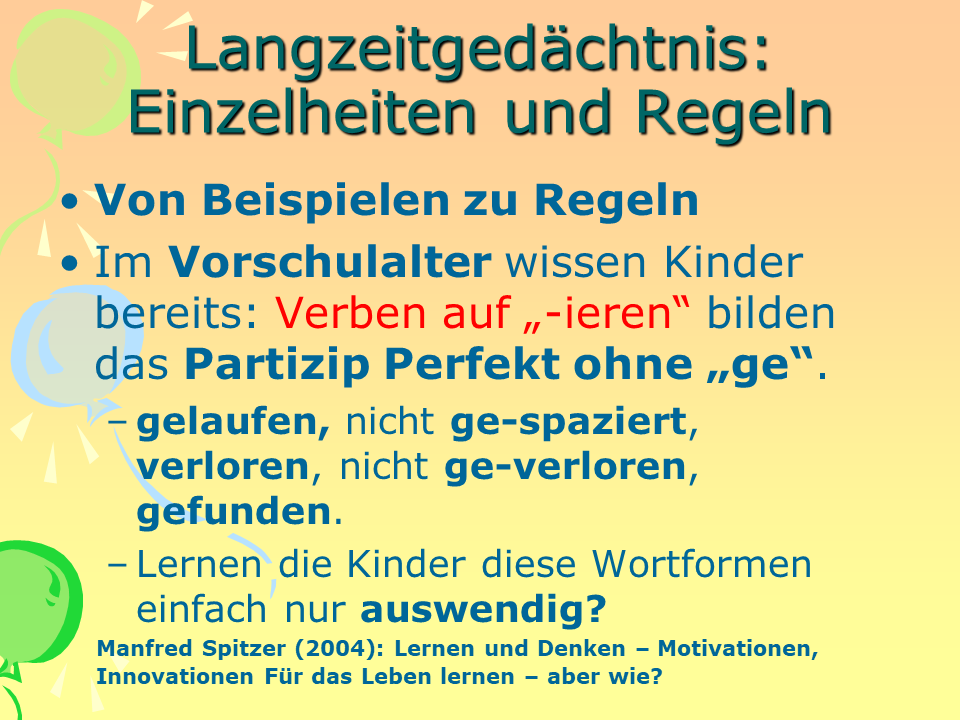
\includegraphics[width=1\textwidth,height=\textheight]{./pictures/neuro/Diapozitiv46.PNG}

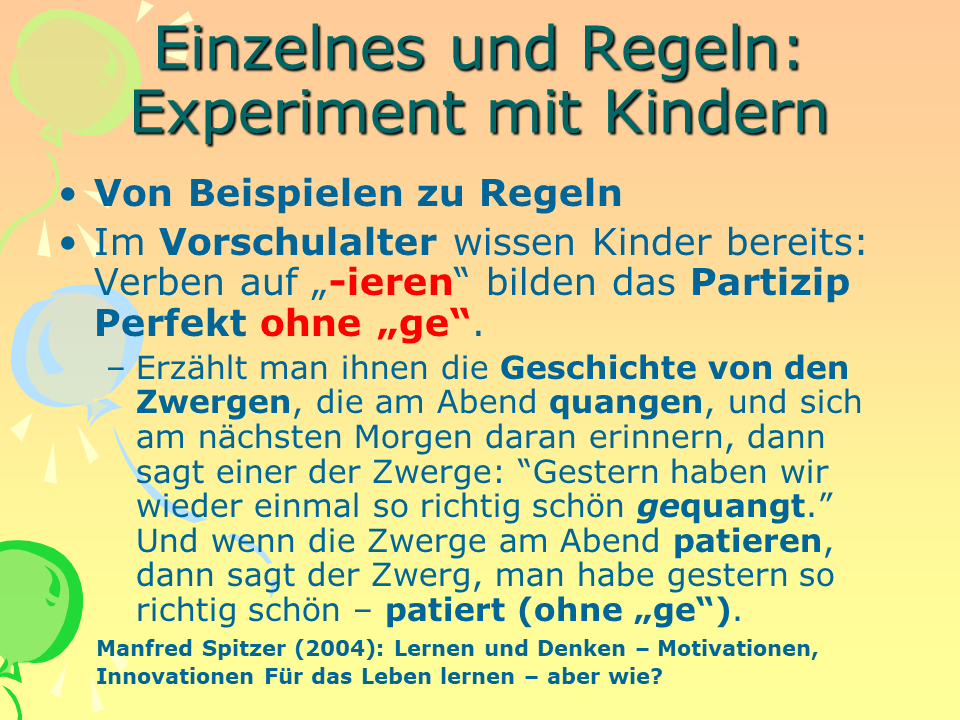
\includegraphics[width=1\textwidth,height=\textheight]{./pictures/neuro/Diapozitiv47.PNG}

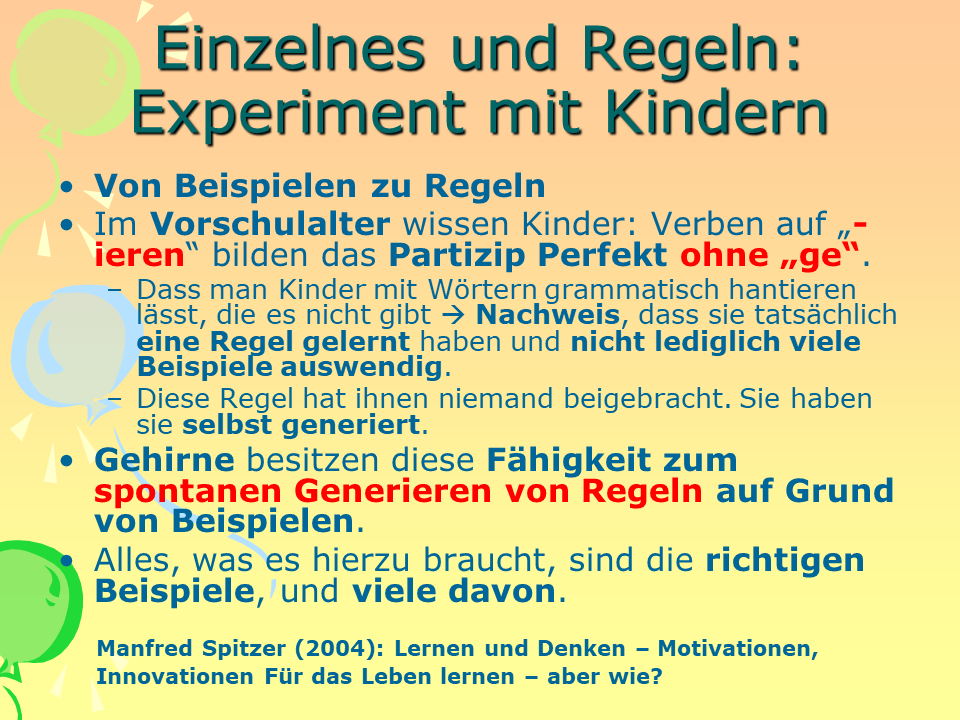
\includegraphics[width=1\textwidth,height=\textheight]{./pictures/neuro/Diapozitiv48.PNG}

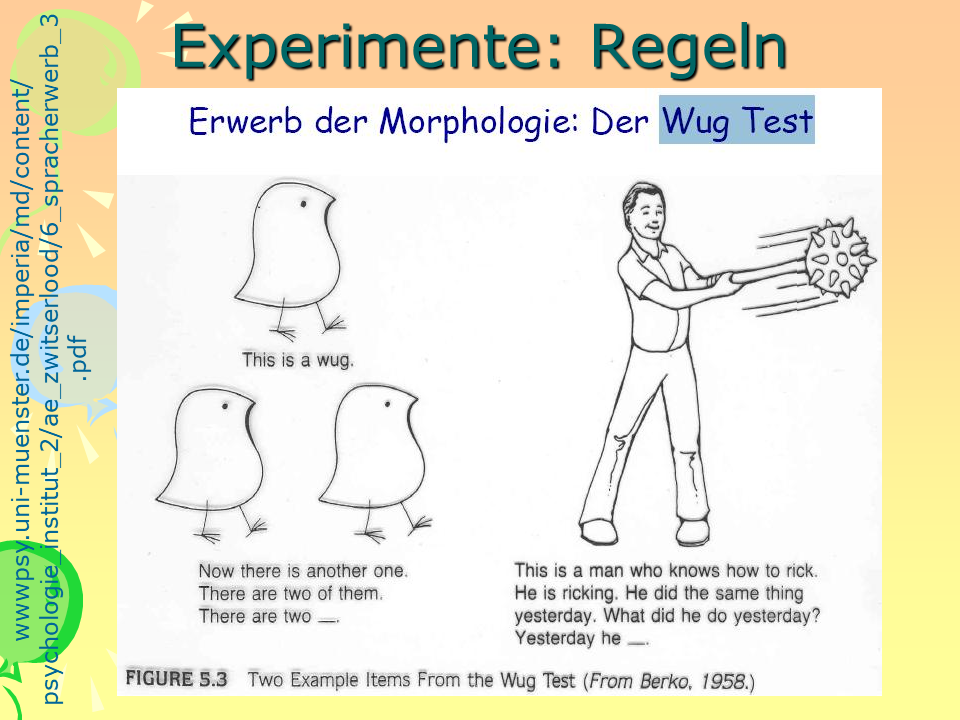
\includegraphics[width=1\textwidth,height=\textheight]{./pictures/neuro/Diapozitiv49.PNG}

\includegraphics[width=1\textwidth,height=\textheight]{./pictures/neuro/Diapozitiv50.PNG}

\hypertarget{einzelheiten}{%
\subsubsection{Einzelheiten}\label{einzelheiten}}

\includegraphics[width=1\textwidth,height=\textheight]{./pictures/neuro/Diapozitiv53.PNG}

\includegraphics[width=1\textwidth,height=\textheight]{./pictures/neuro/Diapozitiv54.PNG}

\includegraphics[width=1\textwidth,height=\textheight]{./pictures/neuro/Diapozitiv55.PNG}

\hypertarget{emotionen}{%
\subsubsection{Emotionen}\label{emotionen}}

Welche Rolle spielen Emotionen beim Lernen?

\includegraphics[width=1\textwidth,height=\textheight]{./pictures/neuro/Diapozitiv57.PNG}

\includegraphics[width=1\textwidth,height=\textheight]{./pictures/neuro/Diapozitiv58.PNG}

\includegraphics[width=1\textwidth,height=\textheight]{./pictures/neuro/Diapozitiv59.PNG}

\includegraphics[width=1\textwidth,height=\textheight]{./pictures/neuro/Diapozitiv60.PNG}

\hypertarget{limbisches-system}{%
\subsubsection{Limbisches System}\label{limbisches-system}}

\includegraphics[width=1\textwidth,height=\textheight]{./pictures/neuro/Diapozitiv61.PNG}

\includegraphics[width=1\textwidth,height=\textheight]{./pictures/neuro/Diapozitiv62.PNG}

\includegraphics[width=1\textwidth,height=\textheight]{./pictures/neuro/Diapozitiv63.PNG}

\begin{itemize}
\item
  \textbf{Sensorisches Gedächtnis} (welche Funktion hat es?)
\item
  \textbf{Arbeitsgedächtnis} (Welche Beschränkungen hat es? Welche
  Funktion hat nach Baddelys Modell (a) die phonetische Schleife, (b)
  der visuelle Notizblock, (c) die zentrale Exekutive? Welche Rolle
  spielt Aufmerksamkeit für die Aufnahme ins Arbeitsgedächtnis? Wie kann
  man die Kapazizät des Arbeitsgedächtnisses steigern?
\item
  Wissenssysteme im \textbf{Langzeitgedächtnis} (Welche auffällige
  Unterschiede gibt es zwischen dem deklarativen und dem prozeduralen
  Langzeitgedächtnis? Welche (sprachlichen oder nicht-sprachlichen)
  Reize (Stimuli) haben größere Chancen, im Langzeitgedächtnis
  gespeichert zu werden? Welchen Einfluss haben emotional geladene Reize
  auf die Speicherung im Langzeitgedächtnis? Welche Funktion haben der
  Hippokampus, die Amygdala und frontale Hirnrindenbereiche in Bezug auf
  die langzeitige Speicherung von Einzelheiten oder Regelmäßigkeiten?)
\end{itemize}

\hypertarget{lernphasen}{%
\section{Lernphasen}\label{lernphasen}}

Warum gibt es Lernphasen?

\includegraphics[width=1\textwidth,height=\textheight]{./pictures/neuro/Diapozitiv65.PNG}

\includegraphics[width=1\textwidth,height=\textheight]{./pictures/neuro/Diapozitiv66.PNG}

\includegraphics[width=1\textwidth,height=\textheight]{./pictures/neuro/Diapozitiv67.PNG}

\hypertarget{alter}{%
\section{Alter}\label{alter}}

Welcher Zusammenhang besteht zwischen biologischem Alter und
Lerngeschwindigkeit?

\includegraphics[width=1\textwidth,height=\textheight]{./pictures/neuro/Diapozitiv70.PNG}

\includegraphics[width=1\textwidth,height=\textheight]{./pictures/neuro/Diapozitiv71.PNG}

\includegraphics[width=1\textwidth,height=\textheight]{./pictures/neuro/Diapozitiv72.PNG}

\includegraphics[width=1\textwidth,height=\textheight]{./pictures/neuro/Diapozitiv73.PNG}

\includegraphics[width=1\textwidth,height=\textheight]{./pictures/neuro/Diapozitiv74.PNG}

\includegraphics[width=1\textwidth,height=\textheight]{./pictures/neuro/Diapozitiv75.PNG}

\hypertarget{einfluss-des-alters-auf-l2}{%
\subsection{Einfluss des Alters auf
L2}\label{einfluss-des-alters-auf-l2}}

\includegraphics[width=1\textwidth,height=\textheight]{./pictures/neuro/Diapozitiv76.PNG}

\includegraphics[width=1\textwidth,height=\textheight]{./pictures/neuro/Diapozitiv77.PNG}

\includegraphics[width=1\textwidth,height=\textheight]{./pictures/neuro/Diapozitiv78.PNG}

\includegraphics[width=1\textwidth,height=\textheight]{./pictures/neuro/Diapozitiv79.PNG}

\includegraphics[width=1\textwidth,height=\textheight]{./pictures/neuro/Diapozitiv80.PNG}

\includegraphics[width=1\textwidth,height=\textheight]{./pictures/neuro/Diapozitiv81.PNG}

\includegraphics[width=1\textwidth,height=\textheight]{./pictures/neuro/Diapozitiv82.PNG}

\includegraphics[width=1\textwidth,height=\textheight]{./pictures/neuro/Diapozitiv83.PNG}

\includegraphics[width=1\textwidth,height=\textheight]{./pictures/neuro/Diapozitiv84.PNG}

\hypertarget{hirnreifeprozess}{%
\subsection{Hirnreifeprozess}\label{hirnreifeprozess}}

\includegraphics[width=1\textwidth,height=\textheight]{./pictures/neuro/Diapozitiv86.PNG}

Aus dem Kapitel \emph{Sprachlernvoraussetzungen: biologische
Voraussetzungen}, von Apeltauer and Boeckmann (1997): 68-76.

\includegraphics[width=1\textwidth,height=\textheight]{./pictures/neuro/Diapozitiv87.PNG}

\includegraphics[width=1\textwidth,height=\textheight]{./pictures/neuro/Diapozitiv88.PNG}

\includegraphics[width=1\textwidth,height=\textheight]{./pictures/neuro/Diapozitiv89.PNG}

\hypertarget{l1-l2-parallelen}{%
\subsection{L1-L2-Parallelen}\label{l1-l2-parallelen}}

Aus dem Kapitel \emph{Sprachlernvoraussetzungen: biologische
Voraussetzungen}, von Apeltauer and Boeckmann (1997): 68-76.

\includegraphics[width=1\textwidth,height=\textheight]{./pictures/neuro/Diapozitiv90.PNG}

\includegraphics[width=1\textwidth,height=\textheight]{./pictures/neuro/Diapozitiv91.PNG}

\includegraphics[width=1\textwidth,height=\textheight]{./pictures/neuro/Diapozitiv92.PNG}

\hypertarget{section-1}{%
\section{}\label{section-1}}

\hypertarget{sec-theorien}{%
\chapter{Markante Thesen einflussreicher
Spracherwerbstheorien}\label{sec-theorien}}

\begin{figure}

{\centering 

\href{https://www.clipartmax.com/middle/m2K9A0m2i8Z5A0i8_more-technology-icon-png/}{\includegraphics[width=1\textwidth,height=\textheight]{./pictures/clipart10912.png}}

}

\end{figure}

Dietrich (2002): Bearbeiten!!!

\hypertarget{soziale-ausstattung-von-menschenkindern}{%
\section{Soziale Ausstattung von
Menschenkindern}\label{soziale-ausstattung-von-menschenkindern}}

\hypertarget{zeigegesten}{%
\subsection{Zeigegesten}\label{zeigegesten}}

Dass Kinder im Säuglingsalter mit Zeigegesten kommunizieren, ist schon
seit Langem bekannt und seit rund 40 Jahren experimentell untersucht
worden (vgl. Bates/Camaioni/Volterra 1975; Lempers 1979). Im hier
gegebenen Zusammenhang sind drei Befunde bedeutsam.

\begin{itemize}
\item
  Das kommunikative Verwenden von Zeigegesten des Kleinkindes
  unterscheidet sich wesentlich von dem von Menschenaffen generell,
  indem es Mittel kooperativer Kommunikation ist, das von Primaten
  hingegen egozentrisch; ausführlich und entwicklungsgeschichtlich wird
  dies beschrieben in Tomasello et al.~(2005).
\item
  Kinder verwenden Zeigegesten zu zwei verschiedenen Aktivitäten:

  \begin{itemize}
  \item
    zum Auffordern (imperative)
  \item
    und zum Erklären (declarative).

    Nach den Befunden von Camaioni/Perucchini/Bellagamba/Colonnesi
    (2004) tritt letztere deutlich nach der ersteren Funktion auf; so
    auch Liebal/ Behne/Carpenter/Tomasello (2009).
  \end{itemize}
\item
  Zum dritten zeigen beide Verhaltensweisen, dass das Kind ab dem Alter
  von ca. vierzehn Monaten die Fähigkeit hat, kommunikativ mit einem
  Erwachsenen zu interagieren und -- im Alter von etwa 18 Monaten -- die
  Aufmerksamkeit des Erwachsenen auf einen von beiden Beteiligten als
  relevant erachteten Sachverhalt zu lenken. Insbesondere in dieser
  Fähigkeit wird übereinstimmend in der Forschung der Vorläufer
  kooperativer sprachlicher Kommunikation gesehen.
\end{itemize}

\hypertarget{biologische-ausstattung}{%
\section{Biologische Ausstattung}\label{biologische-ausstattung}}

Welche körperlichen Eigenschaften und Fertigkeiten erklären die
Möglichkeit des Erwerbs der Sprachfähigkeit des Menschen?

\begin{itemize}
\item
  \textbf{Phylogenetisch} ist zum Nachweis dieser Voraussetzungen sehr
  weit zurückzuschauen, nämlich etwa sechs Millionen Jahre. Das ist nach
  paläoanthropologischer Schätzung das Erdzeitalter, in dem die Bewohner
  der Region in und westlich von Äthiopien sich vom Vierbeiner zum
  Zweibeiner und damit zum aufrechten Gang hin entwickelt haben. Damit
  war die Voraussetzung für die Entwicklung des sog. Ansatzrohres der
  Hominiden gegeben und damit die Fähigkeit einer Dosierung des
  Ausatmungsstroms, wie sie der Gattung Mensch eigen und für die
  Produktion einer gegliederten sprachlichen Äußerung erforderlich ist
  (vgl. Schrenk 2008).
\item
  Damit verbunden ist die \textbf{ontogenetische} Entwicklung des
  Rachenraumes des Menschen im ersten Lebensjahr, wie oben beschrieben;
  d.~h. die Öffnung der Mundhöhle durch Wölbung des Gaumens und die
  Absenkung des Kehlkopfes im Lauf des ersten Lebensjahres. So lässt
  sich vorhersagen, dass hintere Vokale später als vordere erworben
  werden und der vordere Konsonantismus früher als der pharyngale (s.
  Kap. 3.4.1). Bei letzterem ist zudem erklärend die Tatsache relevant,
  dass die Bildung vorderer Konsonanten visueller Wahrnehmung eher
  zugänglich ist, als die der hinteren.\\
\end{itemize}

\hypertarget{kognitive-ausstattung}{%
\section{Kognitive Ausstattung}\label{kognitive-ausstattung}}

Die wissenschaftliche Diskussion darüber, welche angeborene kognitive
Ausstattung der Sprachfähigkeit des Menschen zugrunde liegt, ist
kontrovers und zwar seit etwa einem halben Jahrhundert.

\begin{itemize}
\item
  Wie erklärt es sich, dass kein anderes Lebewesen als der Mensch ein so
  reichhaltiges und vernetztes lexikalisches \textbf{Wissen} und
  dermaßen differenzierte strukturelle Regelhaftigkeiten erwerben kann
  -- und das in einem sonst so unausgereiften Organismus und \textbf{in
  so kurzer Zeit}? Und ohne eine systematische explizite Unterweisung!
\item
  Als sicher ist anzunehmen, dass das leistungsfähige
  \textbf{Gedächtnis}, die damit operierende Fähigkeit der
  Begriffsbildung und Strukturerkennung für die Entwicklung des
  sprachlichen Wissens wesentlich sind.
\item
  Viele Einzelheiten, auch wesentliche, sind aber nur über die
  Beobachtung der Ergebnisse der \textbf{kognitiven} Aktivität
  zugänglich, das heißt durch Interpretation der Denk- und
  Sprachäußerungen des Kindes im Lauf des Spracherwerbs. Das
  \textbf{sprachliche} Verhalten des Kindes bildet also das Fenster,
  durch das wir einen Blick auf Einzelheiten der kognitiven Ausstattung
  werfen, die das Kind bei der Geburt eben für die Entwicklung desselben
  mitbringt.
\end{itemize}

-\/-\/-

\hypertarget{zwei-verschiedene-perspektiven}{%
\section{Zwei verschiedene
Perspektiven}\label{zwei-verschiedene-perspektiven}}

In der neueren Geschichte der Spracherwerbsforschung, im
deutschsprachigen Raum also etwa von Beginn des 20. Jahrhunderts
(Stern/Stern 1909) bis heute, wurde den genannten Umständen und weiteren
mehr ein verschieden hoher Erklärungswert zugemessen. Bei aller Vielfalt
im Einzelnen, konvergieren die Modelle zu zwei im Ansatz verschiedenen
Sichtweisen. Die eine geht von linguistischen Eigenschaften natürlicher
Sprachen aus, die andere von den Herausforderungen, in einer gegebenen
Situation mit der anzunehmenden kognitiven Fähigkeit des Kindes
sprachlich Sachverhalte und Intentionen zu kommunizieren. In der
Fachliteratur hat sich für die erstere die Bezeichnung
›\textbf{Nativismus}‹, für die zweitgenannte
›\textbf{Sprachgebrauchsmodell}‹ (usage based theory) etabliert.\\

\hypertarget{nativistisches-spracherwerbsmodell}{%
\subsection{Nativistisches
Spracherwerbsmodell}\label{nativistisches-spracherwerbsmodell}}

Die Grundannahme der nativistischen Sprachtheorie besagt: Der Mensch ist
genetisch mit einem Sprachorgan ausgestattet und darin unterscheidet er
sich von allen anderen Lebewesen.

Die Kernbehauptung der nativistischen Sprachtheorie, der Mensch sei
genetisch mit einem Sprachorgan ausgestattet, lässt natürlich sofort
Fragen und Zweifel entstehen. Spezialliteratur über den Spracherwerb ist
au- ßer Chomsky (1980) besonders die umfassende Darstellung in Pinker
(1994) und die einschlägigen Teile in dem Handbook of Child Language
(Fletcher/MacWhinney 1995).\\

Das Sprachorgan: Was hat man unter dem oben postulierten Sprachorgan zu
verstehen? Offensichtlich ist es kein chirurgisch identifizierbares,
abgegrenztes Stück spezialisierten Gewebes mit einer einheitlichen,
komplexen Funktion, eben der, die Sprachfähigkeit zu beherbergen. Man
hat es sich vielmehr als ein genetisch verankertes und
neurophysiologisch repräsentiertes Informationssystem vorzustellen, ein
spezielles Wissenssystem. Es ist dem Bewusstsein nicht zugänglich,
ebenso wenig wie die Fä- higkeit, die dem Menschen das räumliche Sehen
ermöglicht. Es ist universal in dem Sinne, dass es die
Gliederungseigenschaften spezifiziert, die allen und genau den
natürlichen Sprachen gemeinsam sind. Es ist modular; das heißt, dass es
als Ganzes mit dem Denken oder dem Artikulieren interagiert. Es steht
dem Kind von Anbeginn des Spracherwerbs an zur Verfügung, und es prägt
im Zusammenspiel mit den sich entwickelnden Wahrnehmungs- und
Denkfähigkeiten des Kindes den Verlauf des Spracherwerbs.\\

\hypertarget{die-vier-wichtigsten-argumente}{%
\subsubsection{Die vier wichtigsten
Argumente}\label{die-vier-wichtigsten-argumente}}

Betrachten wir die Behauptungen dieses Modells etwas genauer, zunächst
die Argumentation dafür, dass ein solches Modul überhaupt existiert.
Direkte Evidenz in dem Sinne, dass im Zentralnervensystem ein
abgegrenztes Teilsystem von neuronalen Zellen, z. B. in der
Großhirnrinde lokal mit klinischen Verfahren zu bestimmen ist, liegt
nicht vor. Die Annahme der Existenz des universalen Sprachprogramms von
Geburt an stützt sich auf Schlussfolgerungen aus verschiedenen
Beobachtungen, die, so die Argumentation, nicht anders als durch die
genannte Annahme zu erklären sind. Es sind im Wesentlichen
Spracherwerbsbeobachtungen und neuerdings experimentelle Befunde aus
Verhaltensexperimenten mit Kleinkindern.

1. \textbf{Unterdeterminiertheit der Grammatik:} Dafür, dass der
Spracherwerb von Anbeginn durch Strukturprinzipien geleitet ist, wird
angeführt, dass in den Äußerungen des Kindes Formen nicht belegt sind,
die aber auf Grund der Äußerungen, die das Kind hört, theoretisch
erwartbar wä- ren. Ein Beispiel stellt die Bildung von Verb-Erst-Fragen
dar.

\begin{longtable}[]{@{}ll@{}}
\toprule()
(3--1) & Die Puppe liegt im Wagen. \\
\midrule()
\endhead
(3--2) & Liegt die Puppe im Wagen? \\
(3--3) & Die Puppe, die kaputt ist, liegt im Wagen. \\
(3--4) & Liegt die Puppe, die kaputt ist, -- im Wagen? \\
(3--5) & *Ist die Puppe, die kaputt --- , liegt im Wagen? \\
\bottomrule()
\end{longtable}

Würde die Regel für die Bildung der Verb-Erst-Frage nach dem einfachen,
linearen Muster gebildet, so dass das erste Verb nach der Nominalphrase
in der Frage dieser voranzustellen ist, wären Sätze wie (3--5) zu
erwarten. Sie sind aber in der Kindersprache nicht belegt. Das wird als
Evidenz dafür angeführt, dass solche Sätze durch Strukturkenntnis des
Kindes ausgeschlossen werden, die ihrerseits schon vor der Entwicklung
des spezifischen einzelsprachlichen grammatischen Wissens vorhanden ist,
in diesem Fall Wissen über die hierarchische Struktur einer Phrase. Die
Voranstellung des ersten finiten Verbs ist also strukturgeleitet und
wird angewendet auf das erste passende Segment nach der Subjektphrase.\\

\begin{enumerate}
\def\labelenumi{\arabic{enumi}.}
\setcounter{enumi}{1}
\tightlist
\item
  \textbf{Kreativitätsargument}: Eine zweite Erwerbsbeobachtung ist,
  dass Kinder Sätze bilden können, die sie zuvor nicht gehört haben.
  Dieses Faktum, so die Argumentation, spricht für ein Strukturwissen,
  dass diese Kreativität ermöglicht.
\end{enumerate}

3. \textbf{Defizienter Input}: Als weiteres Argument wird daraus
abgeleitet, dass das Ergebnis des Spracherwerbs grammatisches, wiederum
unbewusstes Sprachwissen ist, das den Menschen in die Lage versetzt,
wohlgeformte Sätze von nicht wohlgeformten zu unterscheiden, z. B.
(3--8) gegenüber (3--9).

\begin{longtable}[]{@{}ll@{}}
\toprule()
(3--6) & Wer kommt? \\
\midrule()
\endhead
(3--7) & Wer, glaubt Hans, kommt? \\
(3--8) & Welcher Besuch kommt? \\
(3--9) & *Welcher, glaubt Hans, Besuch kommt? \\
\bottomrule()
\end{longtable}

Das ist deshalb erklärungsbedürftig, weil das Kind im Lauf des
Spracherwerbs durchaus auch viele nicht wohlgeformte Sätze und
abgebrochene Äußerungen hört.

4. Das \textbf{Fehlen negativer Evidenz}: Schließlich ein Argument ex
negativo. Es wurde erwähnt, dass die pure lineare Form der
Inputäußerungen erwarten ließe, dass das Kind daraus Muster von
Äußerungen wie (3--5) ableiten würde. Sie sind aber in der Kindersprache
nicht belegt. Nun könnte dieses Fehlen auch damit erklärt werden, dass
dem Kind Hinweise auf abweichende Äußerungen gegeben werden, die den
Erwerb dann in die Zielrichtung steuern. Nach dem Stand der Kenntnis ist
dem aber nicht so. Und eben dieser Umstand des Fehlens negativer Evidenz
aus der Sicht des Kindes stärkt die Annahme, dass es vor dem
Erwerbsbeginn vorhandenes ›Wissen‹ geben muss, dem das Kind bei der
Verarbeitung des Inputs zu spezifischem sprachlichen Wissen folgt.

Für die Beurteilung der nativistischen Konzeption sind zunehmend Befunde
aus experimentellen Untersuchungen und vom Sprachverhalten geistig
kranker Kinder verfügbar geworden. Sie gelten hauptsächlich den Fragen
nach der Modularität des sprachlichen Systems, besonders in Abgrenzung
von bzw. Interaktion mit dem allgemeinen Denkvermögen (vgl. Weinert
2000, bes. Abschnitt 4) und der Existenz universalen sprachspezifischen
Wissens vor dem Erwerb (vgl. Höhle/Weissenborn 1999). Die die
Modularität betreffenden Befunde stärken weder noch widerlegen sie
unbestreitbar die Grundannahmen der nativistischen Konzeption (vgl.
Weinert 2000, Kap. 5). Die psychopathologischen Befunde sprechen eher
für die Unabhängigkeit der Sprachfähigkeit von der sonstigen
Denkfähigkeit. Direkt auf spezifisches sprachliches Wissen gerichtete
Experimente zur rezeptiven Sprachbeherrschung bestätigen allerdings
wiederum, dass Kleinkinder sehr viel früher, als bisher auf Grund von
Produktionsdaten angenommen, für Strukturunterschiede in sprachlichem
Material sensitiv sind (vgl. Höhle/Weissenborn 1999, Kap. 2.3.4 und
2.3.5). Inwiefern das die nativistische Konzeption bestätigt, bleibt
noch zu zeigen.

Das \textbf{UG-Wissen des Kindes:} Was ist, nach Annahme der
nativistischen Theorie, der Inhalt des angeborenen sprachlichen Wissens?
Wie jede Theorie ist auch diese -- bei aller Kontinuität in den
Grundannahmen -- Veränderungen über die Zeit und Unterschieden infolge
unterschiedlicher Sichtweisen einzelner Wissenschaftler ausgesetzt. Das
liegt daran, dass die Beobachtungsdaten aus dem Spracherwerb
Deutungsspielräume zulassen, und an dem Auftauchen neuer Beobachtungen.
Von Varianten abgesehen, ist das angeborene ›Sprachorgan‹ grammatisches
Wissen. Es enthält (unbewusste) Kenntnis über den Aufbau sprachlicher
Ausdrücke, sog. grammatische Prinzipien.\\
\textbf{Parameter}: Nun sind bekanntlich nicht alle Sprachen einheitlich
gebaut; dem trägt die Theorie dadurch Rechnung, dass angenommen wird,
einige der Prinzipien seien parametrisiert. So unterscheiden sich
Sprachen z. B. in der Reihenfolge von X0 und YP, was durch Annahme einer
Hilfsgröße »Kopfposition« im Strukturwissen theoretisch erfasst wird.
Ein Parameter hat endlich viele Werte, der Kopfparameter z. B. zwei
›kopfinitial‹ und ›kopffinal‹. Eine detaillierte Darstellung der derzeit
anzunehmenden Prinzipien und Parameter liefern Stechow/Sternefeld (1988)
und Chomsky/ Lasnick (1993, Kap. 1). Zusammenfassend: Das logische
Problem des Kindes beim Spracherwerb besteht darin, die Parameterwerte
ausfindig zu machen, die in seiner Umgebungssprache ausgeprägt sind.
Erwerbslogisch stellt die Parametrisierung also so etwas dar, wie das
strukturelle Bindeglied zwischen dem universalen sprachlichen Wissen und
den spezifischen Strukturverhältnissen in der jeweiligen
Umgebungssprache. Abgesehen davon, dass sich das Konzept in der
typologischen Forschung zunehmend bestätigt, wurde seine Wirkung auch in
materialreichen Studien des Spracherwerbs aufgezeigt (vgl. die
Synchronie des Erwerbs von Doppel-Nomen-Zusammensetzungen und
Verb-Partikel-Sätzen in der Kindersprache; Snyder 2007)\\

\textbf{Zwei Positionen zum Erwerbsverlauf}: Wie erklärt schließlich die
nativistische Theorie den beobachteten Erwerbsverlauf? Hierzu ist vorab
etwas Grundsätzliches zu berücksichtigen. Es wird streng unterschieden
zwischen dem sprachlichen Wissen des Kindes und dem Vorgang, die
Inputdaten mit dem UG-Wissen in Verbindung zu bringen, was eine Reihe
von Problemlösungen prozeduraler Art impliziert, z. B. das Segmentieren
des Schallstroms in Laute, Silben und Wörter, das Zuordnen von
Wortformen zu Begriffen, das Klassifizieren von Wörtern etc. Vor diesem
Hintergrund kann nun entweder angenommen werden, dass das genetisch
verankerte Wissen von Anbeginn in Gänze vorhanden ist (zur sog. starken
Kontinuitätsannahme s.Pinker 1994) oder dass es -- genetisch gesteuert
-- in den ersten Monaten und Jahren des Spracherwerbs wächst (zur
schwachen Kontinuitätsannahme s. Borer/Wexler, 1987). Auch neuere
experimentelle Befunde stützen diese Annahme (vgl. Friederici 2005).\\

\hypertarget{sprachgebrauchsmodell}{%
\subsection{Sprachgebrauchsmodell}\label{sprachgebrauchsmodell}}

Um das Wesentliche dieses Forschungsprogramms verständlich zu machen,
ist es ratsam, zunächst die anfänglichen Grundannahmen vorzustellen. Es
sind, wie in allen Spracherwerbstheorien, Annahmen über die spezifische
Relevanz von Erwerbsvoraussetzungen; sie finden sich einführend gelistet
in Tomasello (2009: Kapitel 2).

\hypertarget{grundannahmen}{%
\subsubsection{Grundannahmen}\label{grundannahmen}}

Was besagt das »Usage based-Modell« des Spracherwerbs? Zunächst einmal
wird die Existenz von angeborenem universalem sprachbezogenen Wissen des
Kindes kategorisch bestritten. Das Kind, so die Grundannahme, erwerbe
die Sprachfähigkeit durch die aufmerksame, von Neugier und Wissensdrang
getriebene Verwendung der Sprache mit den Erwachsenen seiner
Brutpflegeumgebung.

\hypertarget{kommunikative-fertigkeiten}{%
\subsubsection{Kommunikative
Fertigkeiten}\label{kommunikative-fertigkeiten}}

Es verfüge dazu über die folgenden kommunikativen Fertigkeiten:

\begin{itemize}
\item
  Die Fertigkeit, Aufmerksamkeit auf Gegenstände und Sachverhalte mit
  Kommunikationspartner zu teilen.
\item
  Die Fertigkeit, der Aufmerksamkeit und der Gestik von Personen zu
  folgen, die sich auf entfernte Gegenstände oder Ereignisse außerhalb
  des Bereichs der unmittelbaren Interaktion befinden.
\item
  Die Fertigkeit, selbst die Aufmerksamkeit anderer auf entfernte
  Objekte und Ereignisse zu lenken.
\item
  Die Fertigkeit, kulturgeleitet die absichtsgeleiteten Handlungen
  anderer zu erlernen, einschließlich kommunikativer Aktivitäten und
  ihrer zugrundeliegenden Absichten.
\end{itemize}

Hier finden sich also die oben genannten Merkmale der »\textbf{sozialen
Ausstattung}« des Säuglings wieder.

\hypertarget{kognitive-fuxe4higkeiten}{%
\subsubsection{Kognitive Fähigkeiten}\label{kognitive-fuxe4higkeiten}}

Des Weiteren notwendig und beteiligt an dem Gelingen des Spracherwerbs
sind nach Tomasello die folgenden kognitiven Fähigkeiten:

\begin{itemize}
\item
  Die Fähigkeit, aus der Ähnlichkeit von wahrgenommenen Reizen
  Kategorien von einander ähnlichen Objekten und Ereignissen zu
  abstrahieren.
\item
  Die Fähigkeit, aus sich wiederholenden Mustern von Wahrnehmung und
  Aktion sensomotorische Schemata zu bilden.
\item
  Die Fähigkeit, anhand von beobachteten Wahrnehmungs- und
  Verhaltenssequenzen häufigkeitsbasierte Verteilungen herauszufinden.
\item
  Die Fähigkeit, aus einander ähnlichen Funktionen von einzelnen
  Bestandteilen komplexer Einheiten Analogien zwischen ihnen abzuleiten.
\end{itemize}

\hypertarget{der-kognitivistische-ansatz}{%
\subsection{Der kognitivistische
Ansatz}\label{der-kognitivistische-ansatz}}

\hypertarget{denkfuxe4higkeit}{%
\subsubsection{Denkfähigkeit}\label{denkfuxe4higkeit}}

Kennzeichnend für diese Theorie ist die Annahme, dass die
Sprachfähigkeit und ihre Entwicklung auf der \textbf{Denkfähigkeit} des
Menschen und deren Entwicklung beruhen. ›Beruhen‹ heißt hier, dass die
Sprachentwicklung die \textbf{Entwicklung der Intelligenz} voraussetzt
und zwar so, dass die Entwicklung von sprachlichen Teilfähigkeiten durch
die Entwicklung entsprechender Intelligenzleistungen bedingt und
determiniert ist. Der Spracherwerb stellt demnach eine spezifische
Denkaktivität des Kindes dar, die auf jeweils vorangehenden
nicht-sprachlichen Intelligenzleistungen aufbaut.

\hypertarget{repruxe4sentationsfunktion}{%
\subsubsection{Repräsentationsfunktion}\label{repruxe4sentationsfunktion}}

Der besondere Nutzen der Sprache für das Denken ergibt sich aus ihrer
\textbf{Repräsentationsfunktion}. Das sprachliche Symbol liefert die
Voraussetzung, Vorstellungen im Geist darzustellen, zu kombinieren und
frei von der aktuellen Situation und Anschauung damit geistig zu
handeln. Forschungslogisch muss also zunächst herausgefunden werden, wie
sich die Intelligenz/das Denken des Kindes entwickelt, von der
Sensomotorik über das mentale Repräsentieren von Anschauungen, das
Operieren mit diesen Repräsentationen bis hin zum abstrakten und
formalen Denken z. B. das Erkennen von und Operieren mit logischen
Relationen. Eben dieses Programm bestimmte die Arbeit von Jean Piaget,
wie er selbst in einer knappen Autobiographie mitteilt (vgl. Piaget
1972).

\hypertarget{schema}{%
\subsubsection{Schema}\label{schema}}

Unter einem \textbf{Schema} versteht man Wissens- oder Verhaltensmuster.
\textless http://www.lern-psychologie.de/kognitiv/Piaget1.pdf\textgreater{}

Beispiel: \textbf{Nahrungsschema}

\includegraphics[width=1\textwidth,height=\textheight]{./pictures/piaget_schema.png}

Ein Schema beschreibt, wie man mit einer Einheit (z.B. Brot) umzugehen
hat.

\hypertarget{adaption}{%
\subsubsection{Adaption}\label{adaption}}

Adaption ist der Prozess der Anpassung. Das Individuum (z.B. das Kind)
versucht sich an die Umwelt anzupassen. Der konstruktivistische Ansatz
zwischen zwei Arten der Anpassung: der Assimilation und der
Akkomodation.

\textbf{Assimilation} bedeutet Eingliederung neuer Erfahrungen in ein
bereits bestehendes Schema, \textbf{Akkommodation} bedeutet dagegen die
Erweiterung bzw. Anpassung eines Schemas (also der kognitiven
Strukturen) an eine wahrgenommene Situation, die mit den vorhandenen
Schemata nicht bewältigt werden kann.

\hypertarget{assimilation}{%
\paragraph{Assimilation}\label{assimilation}}

Assimilation (Schwächungsprozesse, durch die neue Erfahrungen in ein
existierendes Schema eingeordnet werden).

\textbf{Beispiel Assimilation}:

Ein Kind hat bereits gelernt, dass

\begin{itemize}
\item
  ein \textbf{Apfel} zum Mund geführt werden muss,
\item
  der Mund geöffnet werden muss und
\item
  ein Stück herausgebissen werden muss.
\end{itemize}

Trifft dieses Kind nun auf eine \textbf{Birne}, assimiliert das Kind
{[}Apfel und Birne sehen schließlich auch ähnlich aus{]} und geht mit
der Birne genau wie mit einem Apfel um.

\includegraphics[width=1\textwidth,height=\textheight]{./pictures/assimilation.png}

\hypertarget{akkomodation}{%
\paragraph{Akkomodation}\label{akkomodation}}

Akkomodation (Verstärkungsprozesse, die ein wahrgenommenes Problem bei
der Verwendung eines Objekts zu umgehen versuchen, indem das
existierende Schema erweitert wird.)

\textbf{Beispiel Akkommodation}:

Der Versuch eines Kindes an einem \textbf{Bauklotz} zu saugen, wird
durch die Assimilation gestützt, wenn der Bauklotz einem essbaren
Gegenstand ähnlich erscheint. Da der Bauklotz jedoch keine Nahrung
beinhaltet, genügt die Assimilation nicht zur Bewältigung dieser
Situation. Das Kind muss akkommodieren: Das Schema wird erweitert.\\

\includegraphics[width=1\textwidth,height=\textheight]{./pictures/akkomodation.png}

\hfill\break
``Kann eine Situation nicht durch bestehende Schemata erfolgreich
bewältigt werden \protect\hyperlink{assimilation}{Assimilation}, so muss
das entsprechende Schema um die neuen Erkenntnisse erweitert werden
{[}Akkommodation{]}.''

\includegraphics[width=1\textwidth,height=\textheight]{./pictures/peanuts_assimilation_akkomodation.png}

``In diesem Beispiel versucht Linus zunächst zu assimilieren: Er
versucht mit dem Keks so umzugehen, wie er es mit Brot gewöhnt ist: Eine
Scheibe Brot kann man biegen. Nach einigen fehlgeschlagenen Versuchen
akkommodiert er: Ein Keks kann nicht mit Brot gleichgestellt werden. Es
handelt sich zwar bei beiden um etwas Essbares und um eine Backware,
dennoch gibt es Unterschiede. Ein Keks ist etwas anderes, als eine
Scheibe Brot - das vorhandene Schema muss erweitert werden
(Akkommodation), da es nicht ausreicht.''
\url{http://www.lern-psychologie.de/kognitiv/Piaget1.pdf}

\hypertarget{funktional-gesteuerter-spracherwerb}{%
\subsubsection{Funktional gesteuerter
Spracherwerb}\label{funktional-gesteuerter-spracherwerb}}

Die kognitivistisch-konstruktivistische Konzeption der Sprachentwicklung
des Kindes ist demnach grundsätzlich als in die \textbf{Entwicklung der
Intelligenz des Kindes}, seiner Neugier und seiner sozialen
Interaktionsfä- higkeit eingebettet zu sehen. Zwar hat im Werk von
Piaget die Beobachtung des Sprachverhaltens des Kindes am Anfang
gestanden (vgl. Piaget 1923); sie war aber ebenso wie bei Preyer und den
Sterns mehr eine Methode, die Entwicklung der kindlichen Psyche, genauer
die Genese des Denkens beim Kind zu untersuchen. Diese weist nach
\textbf{Piaget vier sukzessive Hauptstufen} auf:

\begin{itemize}
\item
  die sensomotorische Stufe,
\item
  die Stufe des anschaulichen Denkens,
\item
  die Stufe des konkret-operativen Denkens
\item
  und -- beim Erwachsenen schließlich -- die Stufe des formal-operativen
  Denkens.
\end{itemize}

Welche Beobachtungen würden diese Konzeption stützen? Man würde z. B.
erwarten, dass der Verwendung von Sprache in der Interaktion ihre
Verwendung in Vorgängen lauten Denkens in der Entwicklung vorangeht und
dass diese Funktion des Sprechens auch prinzipiell erhalten bleibt. Man
würde weiter erwarten, dass eine sprachliche Ausdruckseinheit erst dann
aus dem Input aufgenommen wird, wenn ihr ein Konzept entspricht. Das
muss natürlich nicht die Bedeutung in der Erwachsenensprache sein, aber
jedenfalls eine Vorstellungseinheit im Wissen des Kindes. Und so müsste
es für alle Bestandteile des Sprachsystems sein, die phonologischen,
morphologischen und syntaktischen Mittel; kurz gesagt, die
kognitivistische Konzeption lässt einen sog. \textbf{funktional
gesteuerten Spracherwerb erwarten}.

\hypertarget{lautes-denken}{%
\subsubsection{\texorpdfstring{\textbf{Lautes
Denken}}{Lautes Denken}}\label{lautes-denken}}

Die erstgenannte Erwartung sah Piaget in dem Phänomen des sog.
\textbf{Monologisierens} des vier- bis siebenjährigen Kindes bestä-
tigt. Die beim selbstorganisierten Spielen beobachteten Kinder einer
Kindertagesstätte redeten vor sich hin, ihre Aktivitäten offenbar eher
sprachlich begleitend als mitteilend, obwohl sich die Äußerungen nach
Form und situativen Gegebenheiten nicht von kommunikativer Interaktion
unterschieden (vgl. Piaget 1973).

\hypertarget{objektpermanenz}{%
\subsubsection{\texorpdfstring{\textbf{Objektpermanenz}}{Objektpermanenz}}\label{objektpermanenz}}

Für die Erwartung eines konzeptgesteuerten Erwerbs sprachlicher Mittel
sprechen Beobachtungen zur zeitlichen Reihenfolge von begrifflicher und
sprachlicher Entwicklung. Von Geburt an bis etwa zum Ende des ersten
Lebensjahres ist dem kindlichen Denken ein Objekt nur so lange präsent,
wie es wahrgenommen wird. Erst zwischen 0;10 und 1;0 entwickelt sich die
kognitive Fähigkeit, eine geistige Vorstellung eines Objekts zu
bewahren, die sog. Objektpermanenz. Zeitlich mit ihr einher, genauer
gesagt geringfügig nachzeitig, geht der Erwerb des ersten
bedeutungshaltigen Wortes vonstatten. Sprachliche Mittel für WarumFragen
sind zeitlich an die begriffliche Erkenntnis des Kausalzusammenhangs
gekoppelt und zahlreiche Beobachtungen in Folgeuntersuchungen im Rahmen
des kognitivistischen Paradigmas haben weitere Zusammenhänge zugunsten
des funktionalistischen Modells erbracht.

\hypertarget{nicht-bestuxe4tigte-annahmen}{%
\subsubsection{Nicht bestätigte
Annahmen}\label{nicht-bestuxe4tigte-annahmen}}

Allerdings haben nicht alle Ergebnisse späterer Untersuchungen die
ursprünglichen Annahmen bestätigt. Den generellen Zusammenhang zwischen
kognitivem Niveau und sprachlicher Entwicklung haben
SchanerWolles/Haider (1987) überprüft. Von rund 60 Kindern zwischen 5
und 9 Jahren wurde mit einer standardisierten Testbatterie die
Entwicklung ihres operativen Denkens ermittelt. Parallel dazu wurde mit
einer Satz-BildMatching-Aufgabe ihr Verstehen von Sätzen mit
unterschiedlich komplexen anaphorischen Relationen gemessen. Die
Ergebnisse zeigten einen signifikanten Zusammenhang zwischen dem Alter
und der kognitiven Entwicklung, aber keinen durchgängigen Zusammenhang
zwischen kognitiver und sprachlicher Entwicklung. Damit bestätigen sich
Befunde frü- herer Experimente, besonders von Sinclair-de Zwart (1971).

\hypertarget{bestuxe4tigte-annahmen}{%
\subsubsection{Bestätigte Annahmen}\label{bestuxe4tigte-annahmen}}

Deutlicher positiv ist die Evidenz über den Zusammenhang zwischen der
Struktur der Entwicklung der sensomotorischen Intelligenz und dem Erwerb
semantischer Sprachmittel. So stehen nach Bloom (1973) und Szagun (2013)
Stufen des Syntaxerwerbs mit Stufen der sensomotorischen Entwicklung in
den ersten zwei Lebensjahren insofern in Analogie, als der syntaktischen
Entwicklung die Entwicklung semantischer Konzepte, nämlich der
Kasusrollen im Sinne von Fillmore (1968) zu Grunde liegen, welche
ihrerseits analog zu den Stufen der Sensomotorikentwicklung abläuft.

\hypertarget{operationsprinzipien}{%
\subsubsection{Operationsprinzipien}\label{operationsprinzipien}}

Die Frage, wie das Kind in der ja nicht vorsegmentierten Folge von
Schall die formalen Einheiten erkennt, denen sensomotorischen
Bedeutungen zuzuordnen sind, eine Frage übrigens, die aus der Sicht
jeder Theorie beantwortet werden muss, hat durch die
sprachvergleichenden Erwerbsuntersuchungen von Slobin (1973) eine
kognitivistisch basierte Antwort gefunden. Die vergleichende Analyse von
Erwerbsdaten aus vierzig Sprachen sowie die darauf bezogene
Kategorisierung der Inputeigenschaften führte zur Annahme kognitiver
Prinzipien, denen alle Kinder bei der Segmentierung, Klassifikation und
beim Erkennen grammatischer Beziehungen wahrscheinlich gefolgt sind:
sog. universale Operationsprinzipien.\\

\hypertarget{spracherwerbsdaten-von-ungarisch-serbokroatischen-bilingualen-kindern-vgl.-slobin-1973}{%
\paragraph{Spracherwerbsdaten von ungarisch-serbokroatischen bilingualen
Kindern (vgl. Slobin
1973)}\label{spracherwerbsdaten-von-ungarisch-serbokroatischen-bilingualen-kindern-vgl.-slobin-1973}}

Die Spracherwerbsdaten ungarisch-serbokroatisch bilingualer Kinder
weisen auf, dass die Ausdrücke für die Bezeichnung von Ortsrelationen im
Ungarischen früher gelernt werden als im Serbokroatischen. Zugleich ist
aber klar, dass die Kinder die entsprechenden Konzepte schon haben
müssen, auch wenn sie die sprachlichen Ausdrücke des Serbokroatischen
nicht erworben haben. Sie kommunizieren sie auf anderen,
lernersprachlichen Wegen, durch Wahl geeigneter Verben, durch Bezug auf
kontextuelle Gegebenheiten o. A. Die Analyse der beteiligten Sprachen
ergibt, dass die Ortsbeziehungen im Ungarischen einheitlich durch
monomorphematische Postpositionen ausgedrückt werden, im
Serbokroatischen durch Präpositionen, Nominalflexion oder beides in
Kombination. Aus diesem und den Befunden aller anderen Daten ergibt sich
eine universale Erwerbsbeobachtung: Postverbale und postnominale lokale
Ausdrücke werden früher gelernt als präverbale und pränominale. (vgl.
Slobin 1973, S. 187 ff.) leitet daraus die Existenz des
Operationsprinzips ab: Richte deine Aufmerksamkeit auf das Ende des
Wortes. Auf die gleiche Weise, abgeleitet aus universalen
Erwerbsbeobachtungen, werden weitere Operationsprinzipien erschlossen
(vgl. Slobin 1973, S. 205--206):

\begin{itemize}
\item
  Vermeide Ausnahmen.
\item
  Der Gebrauch grammatischer Ausdrücke soll semantisch gerechtfertigt
  sein.
\end{itemize}

Die kognitivistische Spracherwerbsforschung weist eine große Zahl von
Einzelergebnissen auf, die die semantische Basis des Formenerwerbs mehr
oder weniger direkt belegen; Entwürfe eines kohärenten Modells des
kindlichen Laut-, Wort- und Syntaxerwerbs wurden erst in jüngster Zeit
durch Budwig (1995) vorgeschlagen. Als problemgeschichtliche Einführung
in das Gebiet empfiehlt sich Weinert (2000)\\

-\/-\/-

\hypertarget{nativismus-vs.-gebrauchstheorien}{%
\subsection{Nativismus
vs.~Gebrauchstheorien}\label{nativismus-vs.-gebrauchstheorien}}

Zusammengestellt anhand von: - Stoll (2008)

\includegraphics[width=4.27in,height=\textheight]{./pictures/muster_intentionen/Diapozitiv2.PNG}

\includegraphics[width=4.27in,height=\textheight]{./pictures/muster_intentionen/Diapozitiv3.PNG}

\includegraphics[width=4.27in,height=\textheight]{./pictures/muster_intentionen/Diapozitiv4.PNG}

\includegraphics[width=4.27in,height=\textheight]{./pictures/muster_intentionen/Diapozitiv5.PNG}

\includegraphics[width=4.27in,height=\textheight]{./pictures/muster_intentionen/Diapozitiv6.PNG}

\includegraphics[width=4.27in,height=\textheight]{./pictures/muster_intentionen/Diapozitiv7.PNG}

\includegraphics[width=4.27in,height=\textheight]{./pictures/muster_intentionen/Diapozitiv8.PNG}

\includegraphics[width=4.27in,height=\textheight]{./pictures/muster_intentionen/Diapozitiv9.PNG}

-\/-\/-

\hfill\break
:::rmdrobot

\begin{itemize}
\item
  In welcher Hinsicht unterscheidet sich Chomskys Nativismus von
  kognivistischen und konstruktivistischen Modellen (Piaget, Tomasello)?
\item
  Welche Rolle spielt soziale Interaktion im Spracherwerb?
\item
  Worin zeigt sich, dass Nachahmungsfähigkeiten zwar wichtig sind im
  Spracherwerb, aber zur Erklärung nicht ausreichen?
\item
  Erläutern Sie die menschlichen Fähigkeiten der Mustererkennung, des
  Perspektivenwechsels und der geteilten Aufmerksamkeit im Spracherwerb!
\item
  Welchen Vorteil hat die Einordnung von Erscheinungen in Kategorien?
  Was unterscheidet Basiskategorien (z.B. Hund ) von anderen Kategorien
  (z.B. Tier, Pudel), prototypische Kategorien (z.B. Spatz) von
  nicht-prototypischen (z.B. Strauß)?
\end{itemize}

(--\textgreater{} Kauschke, Teams, \ldots)

:::

\href{https://www.youtube.com/watch?v=JuRChcbD7FY}{Serious Science}
(Dauer: 11:27 Minuten):

\url{https://www.youtube.com/embed/JuRChcbD7FY}

Language Acquisition in Children Ben Ambridge:

https://www.youtube.com/watch?v=I73Ou2wOyy4

Bilingual First Language Acquisition workshop at the University of York:
Prof.~Ben Ambridge:

https://www.youtube.com/watch?v=0rfU1wlRbwE

\part{Erstspracherwerb}

\hypertarget{sec-stadien}{%
\chapter{Erstspracherwerbsstadien}\label{sec-stadien}}

\begin{figure}

{\centering 

\href{https://www.clipartmax.com/middle/m2i8K9K9G6i8b1A0_apple-tree-technology/}{\includegraphics[width=1\textwidth,height=\textheight]{./pictures/clipart46442.png}}

}

\end{figure}

\begin{itemize}
\tightlist
\item
  Welche typischen Stadien sind im Erstspracherwerb unterscheidbar?
  (--\textgreater{} Vgl. Quarks\&Co, Kauschke, Rainer Dietrich 2016)
\end{itemize}

\begin{figure}

{\centering \includegraphics[width=1\textwidth,height=\textheight]{./pictures/Erstsprachliche_Entwicklung_Tab6_Rainer-Dietrich2016.png}

}

\caption{Rainer Dietrich 2016: Sprachentwicklungsstadien}

\end{figure}

\hypertarget{fruxfche-sprachwahrnehmung}{%
\section{Frühe Sprachwahrnehmung}\label{fruxfche-sprachwahrnehmung}}

Gemäß Kauschke (2012) sind Säuglinge Von Geburt an in der Lage,
spezifische Eigenschaften der Umgebungssprache wahrzunehmen, zu
unterscheiden und allmählich für den Aufbau sprachlichen Wissens zu
nutzen.

\begin{figure}

{\centering \includegraphics[width=1\textwidth,height=\textheight]{./pictures/L1_Entwicklung_kauschke_Tab6.png}

}

\caption{Kauschke (2012):}

\end{figure}

Die Entwicklung der Fähigkeiten beginnt bereits vor der Geburt, denn
bereits wenige Tage alte Kinder zeigen eine besondere Hinwendung zu
sprachlichen Reizen. Nuckelexperimente belegten, dass Neugeborene
menschliche Stimmen gegenüber anderen akustischen Reizen (z.B.
Geräuschen oder Musik) und die Stimme der Mutter gegenüber anderen
Stimmen bevorzugen (DeCasper \& Fifer 1980).

\hypertarget{kategoriale-lautwahrnehmung}{%
\subsection{Kategoriale
Lautwahrnehmung}\label{kategoriale-lautwahrnehmung}}

Gemäß Kauschke (2012) sind Säuglinge fähig, Unterschiede zwischen
einzelnen Lauten wahrzunehmen. Die so genannte kategoriale
Lautwahrnehmung ist bereits im ersten Monat ausgeprägt und im Verlauf
der Entwicklung durch eine allmähliche Abnahme der
Differenzierungsfähigkeit für nicht-muttersprachliche Kontraste
gekennzeichnet (Tees 1984).

Mit dem Begriff der \textbf{kategorialen Lautwahrnehmung} wird darauf
verwiesen, dass kontinuierliche akustische Signale von Hörern in
abgegrenzte Lautkategorien unterteilt werden.

Beispielsweise wird ab einem bestimmten Grad der Stimmhaftigkeit des
Anlauts ein /ba/ statt eines /pa/ wahrgenommen.

\begin{tcolorbox}[enhanced jigsaw, arc=.35mm, left=2mm, bottomrule=.15mm, toprule=.15mm, colframe=quarto-callout-note-color-frame, breakable, rightrule=.15mm, opacityback=0, colback=white, leftrule=.75mm]
\begin{minipage}[t]{5.5mm}
\textcolor{quarto-callout-note-color}{\faInfo}
\end{minipage}%
\begin{minipage}[t]{\textwidth - 5.5mm}

Beispiel Eimas und Kollegen (1971, 1974) präsentierten Säuglingen einen
bestimmten Plosiv, bis durch die Abnahme der Saugrate eine Gewöhnung
angezeigt wurde. Daraufhin wurde der zweite Laut eingespielt und
gemessen, ob bzw. in welchem Ausmaß es zu einer Veränderung der Saugrate
kam. Kinder zwischen einem und vier Monaten konnten stimmhafte und
stimmlose Laute sowie Laute mit verschiedenen Artikulationsorten (/d/
versus /ɡ/) kategorial unterscheiden.

\end{minipage}%
\end{tcolorbox}

Für die Differenzierung von \emph{Frikativen} benötigen sie etwas
länger.

Die Fähigkeit zur kategorialen Lautwahrnehmung bedeutet, dass Säuglinge
phonetische Unterschiede innerhalb einer Phonemkategorie ignorieren,
aber Übergänge von einem Phonem zu einem anderen wahrnehmen, auch wenn
die phonetischen Unterschiede gering sind.

Interessant ist, dass sie sogar lautliche Kontraste unterscheiden
können, die in der eigenen Muttersprache keine bedeutungsunterscheidende
Funktion einnehmen, während diese Fähigkeit bei Erwachsenen nicht mehr
zu beobachten ist. Erwachsene erkennen nur die Kontraste, die für ihre
Sprache relevant sind.

\begin{tcolorbox}[enhanced jigsaw, arc=.35mm, left=2mm, bottomrule=.15mm, toprule=.15mm, colframe=quarto-callout-note-color-frame, breakable, rightrule=.15mm, opacityback=0, colback=white, leftrule=.75mm]
\begin{minipage}[t]{5.5mm}
\textcolor{quarto-callout-note-color}{\faInfo}
\end{minipage}%
\begin{minipage}[t]{\textwidth - 5.5mm}

Beispiel: Im Gegensatz zu japanischen Säuglingen fehlt erwachsenen
japanischen Sprechern die Differenzierungsfähigkeit zwischen den
Phonemen /l/ und /r/, denn diesem Kontrast kommt im Japanischen keine
bedeutungsunterscheidende Funktion zu.

\end{minipage}%
\end{tcolorbox}

Gegen Ende des ersten Lebensjahres vollzieht sich eine \emph{Entwicklung
von der universellen zur einzelsprachlich beeinflussten Wahrnehmung}
(Höhle 2004: 4).

\hypertarget{segmentation}{%
\subsection{Segmentation}\label{segmentation}}

Gemäß Kauschke (2012) ist die \textbf{Segmentation}, also die Zerlegung
des kontinuierlichen Sprachstroms in einzelne Einheitenein weiterer
wesentlicher Schritt, der den Spracherwerb einleitet und ermöglicht.
Auch diese Fähigkeit, die notwendig zum Erkennen von Wortgrenzen und
damit zum Aufbau der grundlegenden Einheiten der Sprache ist, entwickelt
sich im ersten Lebensjahr (für einen Überblick siehe Jusczyk 1999, Höhle
2004).

Die Erwerbsaufgabe der Wortsegmentation ist keineswegs trivial, wenn man
bedenkt, dass Anfang und Ende von Wörtern in der gesprochenen Sprache
nicht explizit durch Pausen oder andere klare Grenzsignale markiert
werden. Die Anforderung an das Kind lässt sich durch die Analogie mit
einem \emph{erwachsenen} Sprecher verdeutlichen, der erstmals eine
gänzlich unbekannte \emph{Fremdsprache} hört und zunächst nicht in der
Lage ist, dem Input Sinneinheiten zu entnehmen (vgl. Höhle 2005).

Das \emph{Segmentieren} des kontinuierlichen Lautstroms und das
Extrahieren von zusammengehörigen Einheiten aus diesem ist eine
notwendige \emph{Voraussetzung für das Wortlernen}, bei dem das Kind
zuvor isolierte und gespeicherte lautliche Einheiten mit Bedeutungen in
Verbindung bringen muss.

Um Grenzen im Sprachstrom zu setzen und Wörter als feste Einheiten zu
erkennen, beachtet das Kind unterschiedliche Hinweisreize, die der Input
bietet, wobei \emph{prosodische Informationen} auch hier zunächst im
Vordergrund stehen. Kinder nutzen vor allem rhythmische Merkmale zur
Gliederung akustischer Signale.

Ab sechs Monaten präferieren sie das \emph{dominante Betonungsmuster}
der Muttersprache und gelangen so zu einem ersten Anhaltspunkt über
mögliche Wortgrenzen. Im Deutschen ist das vorherrschende
Wortbetonungsmuster der \emph{Trochäus}, d.h. eine Abfolge mit einer
betonten und einer unbetonten Silbe.

Das Erkennen der muttersprachlichen Wortbetonung bietet eine
Hilfestellung dahingehend, dass das Kind nun annehmen kann, dass Wörter
in der Regel mit betonten Silben beginnen und eine Wortgrenze daher vor
einer betonten Silbe liegen muss. Diese metrische Strategie erlaubt
einen effektiven Einstieg in die Wortsegmentation, würde aber zu
Fehlinterpretationen führen (z.B. bei Wörtern mit vom Trochäus
abweichenden Betonungsmustern), wenn sie ausschließlich die Wahrnehmung
leitete.

\emph{Weitere}, mit etwa neun Monaten genutzte
\emph{Informationsquellen} für die Segmentierung sind
\emph{phonotaktische Regularitäten.}

Kinder sind in dieser Phase sensitiv dafür, dass nur bestimmte
\emph{Konsonantenfolgen} innerhalb eines Wortes, z.B. als
\emph{wortinitiales} Konsonantencluster, erlaubt sind. Treten davon
abweichende Konsonantenfolgen im Sprachstrom auf, wie z.B. /tk/, so
spricht dies für eine Wortgrenze zwischen diesen Segmenten (wie z.B. in
der Wortfolge ›geht Karl‹, Beispiel aus Pelzer 2011).

Ähnliche Informationen liefern \emph{allophonische Varianten} von
Phonemen. Im Deutschen kann beispielsweise der {[}ç{]}-Laut wortinitial
nicht in der allophonischen Variante des {[}x{]} auftreten, sodass vor
{[}x{]} keine Wortgrenze angenommen werden kann. Somit ist die
distributionelle Analyse des sprachlichen Inputs ein weiteres Mittel,
das zur Segmentierung genutzt werden kann.

\emph{Experimente} mit der Methode des Kopfdrehparadigmas erbrachten
darüber hinaus den Nachweis, dass Kinder mit sieben bis acht Monaten
vorgegebene Inhalts- und hochfrequente \emph{Funktionswörter}
wiedererkennen.

Wurden Kinder eingangs mit einem \emph{Nomen} wie ›\emph{Pinsel}‹ oder
einer \emph{Präposition} wie ›\emph{bis}‹ familiarisiert, so
orientierten sie sich später länger zu Texten hin, die dieses Wort
enthielten (Höhle \& Weissenborn 2003, Höhle 2005). Dies zeigt
eindrücklich, dass sie die Wörter mental speichern und in einem
kontinuierlichen Input wiederentdecken konnten.

Die \emph{Speicherung hochfrequenter Wörter} kann wiederum \emph{als
Segmentierungshilfe} dienen: Erkennt das Kind im Sprachstrom ein bereits
vertrautes und häufig vorkommendes Wort wieder (unabhängig davon, ob ihm
die Bedeutung bekannt ist), so kann es vor und nach diesem Wort eine
Wortgrenze annehmen.

Auch der \emph{eigene Name}, den Kinder mit etwa vier Monaten
wiedererkennen, kann als ein solcher »Ankerpunkt« dienen (Höhle 2004,
Bortfeld et al.~2005).

Nachdem zunächst die rhythmisch-metrische Segmentierungsstrategie
vorherrscht und die Prosodie damit im Sinne des \emph{prosodischen
bootstrappings} den \emph{Einstieg in die Sprachverarbeitung}
ermöglicht, lernt das Kind in der zweiten Hälfte des ersten
Lebensjahres, verschiedene Informationstypen zu integrieren.

Zwischen sieben und elf Monaten schreitet die Fähigkeit,
\emph{vielfältige Hinweise} aus dem Input zur erfolgreichen
Wortsegmentation zu nutzen voran, so dass am Ende dieser
Entwicklungsphase auch Wörter mit einem für die Muttersprache
\emph{untypischen Betonungsmuster} erkannt werden (Jusczyk 1999).

Eine weitere Segmentationsleistung über das Worterkennen hinaus ist das
\emph{Erkennen von größeren syntaktischen Einheiten}. Für den
Grammatikerwerb ist es grundlegend, wichtige strukturelle Einheiten wie
Phrasen und Sätze als zusammengehörig wahrzunehmen.

Innerhalb dieser Domänen werden grammatische Beziehungen wie z.B.
\emph{Subjekt-Verb-Kongruenz} realisiert, die für die Interpretation
eines Satzes von großer Bedeutung sind. Die Grenzen dieser Einheiten
sind \emph{oft durch prosodische Merkmale} wie Pausen, Vokallängung oder
Veränderungen der Stimmfrequenz \emph{gekennzeichnet}.

\begin{tcolorbox}[enhanced jigsaw, arc=.35mm, left=2mm, bottomrule=.15mm, toprule=.15mm, colframe=quarto-callout-note-color-frame, breakable, rightrule=.15mm, opacityback=0, colback=white, leftrule=.75mm]
\begin{minipage}[t]{5.5mm}
\textcolor{quarto-callout-note-color}{\faInfo}
\end{minipage}%
\begin{minipage}[t]{\textwidth - 5.5mm}

Kinder mit unterschiedlichen Muttersprachen präferieren im Alter von
sieben bis zehn Monaten Texte mit natürlichen Pausen an den Satzgrenzen
gegenüber Texten, die künstliche, unsinnige Pausen enthalten
(Hirsh-Pasek et al.~1987).

\end{minipage}%
\end{tcolorbox}

\begin{tcolorbox}[enhanced jigsaw, arc=.35mm, left=2mm, bottomrule=.15mm, toprule=.15mm, colframe=quarto-callout-note-color-frame, breakable, rightrule=.15mm, opacityback=0, colback=white, leftrule=.75mm]
\begin{minipage}[t]{5.5mm}
\textcolor{quarto-callout-note-color}{\faInfo}
\end{minipage}%
\begin{minipage}[t]{\textwidth - 5.5mm}

Schmitz (2009) untersuchte mit dem Kopfdrehparadigma, ob auch Deutsch
lernende Kinder sensitiv gegenüber der Pausendauer sind und das
Vorkommen von \emph{Pausen als Hinweis} auf eine \emph{Satzgrenze}
nutzen. Dazu wurden Satzblöcke mit unterschiedlich langen Pausen
vorgespielt, wobei die Pausen entweder in natürlicher Form zwischen den
Sätzen oder aber mitten in einer Phrase auftraten. Es zeigte sich, dass
sechs Monate alte Kinder zwischen beiden Bedingungen unterscheiden
konnten, also bereits Wissen darüber aufgebaut haben, an welcher Stelle
Pausen adäquat sind. Auch die angemessene Dauer von Pausen wurde
wahrgenommen, denn acht Monate alte Kinder bevorzugten Sätze, in denen
die Pause zwischen zwei Teilsätzen etwas kürzer war als die zwischen
zwei eigenständigen Sätzen, gegenüber Sätzen mit einer umgekehrten und
damit unnatürlichen Abstufung der Pausenlänge. Daraus kann gefolgert
werden, dass \emph{Kinder} in diesem Alter eine »\emph{natürliche
Pausenhierarchie}« (Schmitz 2009: 34) \emph{entdeckt haben}, die ihnen
\emph{helfen} kann, \emph{syntaktisch relevante Einheiten zu erkennen}.

\end{minipage}%
\end{tcolorbox}

\hypertarget{weitere-phonologische-entwicklung}{%
\subsection{Weitere phonologische
Entwicklung}\label{weitere-phonologische-entwicklung}}

\hypertarget{laut--und-phoneminventar}{%
\subsubsection{Laut- und
Phoneminventar}\label{laut--und-phoneminventar}}

Gemäß Kauschke (2012): 34 sind folgende Beobachtungen gemacht worden:

Da \emph{Wortformen} in der frühen Phase \textbf{ganzheitlich} als
holistische Lautgestalten gespeichert werden, erscheinen die
\emph{Phoneme anfangs undeutlich} und unklar, die
\emph{suprasegmentalen} Eigenschaften für das ganze Wort klingen
\emph{jedoch zielsprachlich}. Es kann auch vorkommen, dass einzelne
\emph{Wörter} als ganze Gestalt oder »artikulatorische Geste«
\emph{reproduziert} werden und bereits der korrekten Form der
Zielsprache entsprechen, obwohl sie in der folgenden Phase der
\textbf{segmentorientierten Verarbeitung wieder vereinfacht} werden.
Dieser vermeintliche Rückschritt zeigt einen Umschwung in der Art der
phonologischen Repräsentationen an.

Das anfänglich noch eingeschränke Inventar an Lauten wird allmählich
erweitert.

\begin{tcolorbox}[enhanced jigsaw, arc=.35mm, left=2mm, bottomrule=.15mm, toprule=.15mm, colframe=quarto-callout-note-color-frame, breakable, rightrule=.15mm, opacityback=0, colback=white, leftrule=.75mm]
\begin{minipage}[t]{5.5mm}
\textcolor{quarto-callout-note-color}{\faInfo}
\end{minipage}%
\begin{minipage}[t]{\textwidth - 5.5mm}

Wie sich dies im \emph{Deutschen} vollzieht, zeigen Studien von
Fox-Boyer (Fox-Boyer 2009, siehe auch Fox \& Dodd 1999), in denen Kinder
verschiedener Altersstufen aufgefordert wurden, Bilder zu benennen. Die
Produktionen der Kinder wurden aufgezeichnet und anschließend
transkribiert und bewertet. Auf diese Weise wurde festgestellt, welche
Laute im Inventar der Kinder enthalten waren und in welcher Reihenfolge
phonologische Prozesse überwunden wurden.

\end{minipage}%
\end{tcolorbox}

In Bezug auf das \emph{Lautinventar} wurden das phonetische und das
phonemische Inventar unterschieden. Als \emph{phonetisch erworben} galt
ein Laut, wenn die Mehrzahl der Kinder diesen korrekt artikulieren
konnte, unabhängig davon, ob der Laut in diesem Kontext funktional
angemessen ist (hier wäre das Auftreten von /t/ im Wort ›Tuh‹ statt
›Kuh‹ ein Beleg für die Fähigkeit, den Laut /t/ phonetisch zu
realisieren).

Beim \emph{phonemischen Inventar} hingegen mussten die Kinder den Laut
korrekt in seinem jeweiligen Wortkontext anwenden (z.B. /k/ in ›Kuh‹).
Nach dem Kriterium, dass 90\% der untersuchten Kinder die Laute erworben
haben müssen, ergibt sich folgende \emph{Erwerbsreihenfolge} für die
Vervollständigung des Lautinventars im \emph{Deutschen}:

\begin{figure}

{\centering \includegraphics[width=1\textwidth,height=\textheight]{./pictures/L1_Entwicklung_kauschke_Tab7.png}

}

\caption{Kauschke (2012): 34}

\end{figure}

\emph{Je mehr Laute} produziert werden können, umso \emph{besser} können
\emph{phonologische Prozesse überwunden} werden.

\hypertarget{phonologische-prozesse}{%
\subsubsection{Phonologische Prozesse}\label{phonologische-prozesse}}

In Kauschke (2012): 35 sind folgende Erläuterungen zu finden:

In einem \emph{Reorganisationsprozess}, der mit etwa 18 Monaten beginnt,
weicht die anfänglich holistische Speicherung von Wörtern einer
segmentorientierten Verarbeitung.

Erkennbar ist dies an systematischen \emph{Vereinfachungsprozessen}, die
als regelhafte Abweichungen von den zielsprachlichen Wortformen zu
beschreiben sind. Die Vereinfachungen der Zielsprache lassen sich
systematisch erfassen und mit Hilfe so genannter \emph{phonologischer
Prozesse} klassifizieren (siehe Tabelle 8). Grob gesagt bestehen
phonologische Prozesse darin, dass die korrekte Wortform durch
Auslassung oder Ersetzung von Lauten modifiziert wird.

Bei \emph{Strukturprozessen} wird die gesamte Struktur eines Wortes
verändert, indem z.B. Silben ausgelassen werden; oder die Silbenstruktur
wird durch Auslassung oder Hinzufügung von Lauten modifiziert.

Bei \emph{Substitutionsprozessen} werden Laute durch andere ersetzt.

Wird durch die Lautersetzung eine Angleichung der Lautmerkmale innerhalb
eines Wortes herbeigeführt, spricht man von Harmonisierungs- oder
\emph{Assimilationsprozessen}.

Zu beachten ist, dass phonologische Prozesse hier als Mittel der
Beschreibung zu verstehen sind, mit deren Hilfe die beobachtbaren,
regelhaften Unterschiede zwischen kindlichen und zielsprachgemäßen
Wortformen verdeutlicht und systematisiert werden können (Rothweiler
2002: 261).

\begin{figure}

{\centering \includegraphics[width=1\textwidth,height=\textheight]{./pictures/L1_Entwicklung_kauschke_Tab8.png}

}

\caption{Kauschke (2012): 36}

\end{figure}

In der erwähnten Studie von Fox-Boyer (2009) ergab sich folgende
\emph{Reihenfolge für die Überwindung phonologischer Prozesse}, wobei
hier nur typische Prozesse berücksichtigt wurden, die in der jeweiligen
Altersstufe bei mindestens 10\% aller Kinder auftraten (siehe Tabelle
9).

\begin{figure}

{\centering \includegraphics[width=1\textwidth,height=\textheight]{./pictures/L1_Entwicklung_kauschke_Tab9.png}

}

\caption{Kauschke (2012):}

\end{figure}

\emph{Phonologische Prozesse zeigen} an, dass Abweichungen von der
Zielsprache in der Aussprache von Kindern nicht zufällig sind, sondern
\emph{einem System folgen} (z.B. Vorverlagerung der Velare oder
Plosivierung von Frikativen).

Die \emph{Phase der Inkonsequenz} wird in der zweiten Hälfte des dritten
Lebensjahres überwunden (Schäfer \& Fox 2006), die \emph{Wortformen}
werden danach stabiler und \emph{konsistenter}, auch wenn sie noch von
zielsprachlichen Formen abweichen.

Diese allmähliche Überwindung der phonologischen Vereinfachungsprozesse
bedeutet, dass das phonologische System mehr und mehr zielsprachlich
organisiert wird und die notwendigen distinktiven Merkmale
berücksichtigt werden.

\hypertarget{lexikalische-entwicklung}{%
\subsection{Lexikalische Entwicklung}\label{lexikalische-entwicklung}}

Der Erwerb eines Wortes in seiner Gesamtheit erfordert die aufeinander
bezogene Speicherung von phonologischen, syntaktischen, morphologischen,
semantischen und pragmatischen Informationen. (Kauschke 2012:)

Da der Übergang von der frühen Phase zur darauf folgenden zeitlich mit
der Entwicklung syntaktischen Wissens einhergeht, hat man die beiden
Phasen bezeichnet als:\\
- \emph{vorsyntaktische} (lexikalische, prämorphologische, ca. vor 18.
Lebensmonat) und\\
- \emph{syntaktische Phase des Wortschatzerwerbs} (ca. ab 18.
Lebensmonat). (Dietrich 2016: 79)

\hypertarget{wortverstuxe4ndnis}{%
\subsubsection{Wortverständnis}\label{wortverstuxe4ndnis}}

In den letzten Monaten des ersten Lebensjahres setzt das Wortverständnis
in diesem Sinne ein, nun erkennt das Kind nicht mehr nur die Wortform
wieder, sondern es verknüpft sie mit Bedeutung. (Kauschke 2012:)

\begin{tcolorbox}[enhanced jigsaw, arc=.35mm, left=2mm, bottomrule=.15mm, toprule=.15mm, colframe=quarto-callout-note-color-frame, breakable, rightrule=.15mm, opacityback=0, colback=white, leftrule=.75mm]
\begin{minipage}[t]{5.5mm}
\textcolor{quarto-callout-note-color}{\faInfo}
\end{minipage}%
\begin{minipage}[t]{\textwidth - 5.5mm}

Bates et al.~(1995) stellten durch Elternbefragungsmethoden fest, dass
Kinder mit acht Monaten 36 Wörter und mit 16 Monaten bereits 190 Wörter
verstanden, wobei die individuelle Varianz recht groß war (mit 16
Monaten Spannweite 78 bis 303 Wörter).

\end{minipage}%
\end{tcolorbox}

Der rezeptive Wortschatz von sechsjährigen Kindern wird auf 9000 bis
14000 Wörter geschätzt. Diese quantitative Entwicklung des rezeptiven
Vokabulars zeugt für die beachtliche Fähigkeit von Kindern, schnell und
effektiv eine wachsende Vokabularmenge zu erwerben. (Kauschke 2012:)

Für die Fähigkeit, neue Wörter schnell mit Bedeutungen zu koppeln, auch
wenn der Bedeutungsgehalt noch nicht voll ausdifferenziert ist, führte
Carey (1978) die Bezeichnung \emph{fast mapping} ein. Dieser wirksame
Mechanismus ermöglicht, dass Kinder sofort nach möglichen Bedeutungen
suchen, wenn sie auf eine neue Wortform treffen. Sie legen dann einen
ersten, rudimentären Lexikoneintrag an, der im Laufe der Zeit weiter
ausdifferenziert und durch weitere Informationen angereichert wird.
(Kauschke 2012:)

Im Wortschatzerwerb bezeichnet \emph{fast mapping} die Anwendung einer
speziellen Aufnahmestrategie, die darin besteht, teilweise
unvollständige lautliche Informationen mit teilweise unvollständigen
Bedeutungsvorstellungen zu assoziieren und im mentalen Lexikon zu
speichern. (Dietrich 2016: 83)

Entscheidend sind die \emph{Gedächtnisfunktionen}. Das Kind muss ein in
seiner Umgebung \emph{wiederkehrendes lautliches Gebilde} so gespeichert
haben, dass es dieses in wechselnden Ausprägungen erkennt, mit einer
\emph{konstanten nichtlautlichen Vorstellung} von seiner
\emph{Verwendungsbedingung} (Situation, Ereignistyp, Sache,
Situationsmerkmalen) assoziiert und schließlich auch artikulieren kann.
(Dietrich 2016: 79)

Soweit es Letzteres nicht kann, ist die lexikalische Einheit eben noch
nicht aktiv, sondern nur passiv beherrscht. Alle Beobachtungen sprechen
dafür, dass die \emph{passive Beherrschung der aktiven zeitlich deutlich
vorausgeht}. (Dietrich 2016: 79)

Für die hier geschilderten Prozesse spielen natürlich auch
\emph{Gedächtnisfähigkeiten} eine Rolle. Bevor Informationen ins
Langzeitgedächtnis gelangen, werden sie im \emph{Arbeitsgedächtnis},
auch Kurzzeitgedächtnis genannt (Schwarz 2008: 102f),
zwischengespeichert. (Kauschke 2012:)

Bezogen auf das Wortlernen bedeutet dies, dass dem \emph{phonologischen
Kurzzeitgedächtnis} eine große Bedeutung für den Wortschatzerwerb
zukommt, denn Wortformen müssen hier zunächst verarbeitet werden, bevor
sie in das \emph{mentale Lexikon}, d.h. in den \emph{Langzeitspeicher}
für Wörter, eingehen (zur Rolle des phonologischen Gedächtnisses für den
Lexikonerwerb siehe auch Rothweiler 2001 und Weinert 2004). Das
phonologische Arbeitsgedächtnis stellt damit einerseits eine
\emph{Voraussetzung für den Erwerb und die Speicherung von Wortformen}
dar, wird aber andererseits selbst durch zunehmendes Sprachwissen
beeinflusst. So zeigt Weinert (2004), dass die Arbeitsgedächtnisleistung
sechsjähriger Kinder durch den Wortschatzumfang mit fünf Jahren
vorhergesagt werden kann. (Kauschke 2012:)

Die mit dem Lautgebilde assoziierte Vorstellung ist mit der
Zielbedeutung nicht gleichzusetzen.

\emph{Überdehnung} (Spezialfall der \emph{Übergeneralisierung}): Mit
einem Namen kann sich mehr als die Vorstellung der Person verbinden, die
ihn trägt,\\
- z. B. eine typische Handlung, eine typische Situation; mit einem Wort
wie \emph{heiß} kann sich die Erfahrung des Wehtuns verbinden, das
Verbot, heiße Ding zu berühren oder der Anblick einer offenen
Feuerstelle.\\
\emph{Unterdehnung}: häufiger, aber schwerer nachzuweisen. (Dietrich
2016: 80)

Die \emph{vorsyntaktische (prämorphologische) Phase des
Wortschatzerwerbs} ist gekennzeichnet von einem relativ langsamen Erwerb
von Wörtern, wobei die Aufmerksamkeit des Kindes auf die Wortbedeutung
und weniger auf die morphosyntaktischen Eigenschaften der gelernten
Wörter gerichtet ist. Sie erstreckt sich zeitlich bis zum Alter von ca.
18 Monaten. (Dietrich 2016: 81)

In der \emph{syntaktischen (protomorphologische) Phase des
Wortschatzerwerbs}, die um das Alter von 18 Monaten beginnt und durch
das Auftreten von Mehrwortsätzen gekennzeichnet ist, richtet sich die
Aufmerksamkeit des Kindes verstärkt auf die morphosyntaktischen
Eigenschaften von Wörtern. (Dietrich 2016: 82)

\begin{tcolorbox}[enhanced jigsaw, arc=.35mm, left=2mm, bottomrule=.15mm, toprule=.15mm, colframe=quarto-callout-note-color-frame, breakable, rightrule=.15mm, opacityback=0, colback=white, leftrule=.75mm]
\begin{minipage}[t]{5.5mm}
\textcolor{quarto-callout-note-color}{\faInfo}
\end{minipage}%
\begin{minipage}[t]{\textwidth - 5.5mm}

Feststellungen zur \emph{Überrepräsentation nominaler gegenüber verbaler
Einheiten} (nach Kauschke (2007):\\
- In der Rede von Erwachsenen zu Kindern überwiegen in vielen Sprachen
die Verbtypes.\\
- Unter den gleichen Bedingungen überwiegen innerhalb der Verbtypes die
transitiven gegenüber den intransitiven; vgl. auch
Childers/Tomasello/Hirsh-Pasek/Golinkoff (2006), die spezifisch die
Rolle der Argumentstruktur untersuchen.\\
- Es gibt eine Interaktion zwischen Wortklasse und Aufgabe; die Verb /
Nomen-Differenz ist beim Benennen stärker ausgeprägt als beim
Erkennen.\\
- Bei Kindern gibt es einen Erwerbsfortschritt; die Benenngenauigkeit
nimmt von 2;6 bis 8 zunächst zu, flacht dann aber ab. Die Nomina werden
besser verarbeitet als die Verben.\\
- Genauigkeit und Geschwindigkeit sind beim Benennen mit Nomina besser
als beim Benennen mit Verben, bei Kindern wie bei Erwachsenen.\\
- Auch beim Verstehen gibt es eine Interaktion zwischen Aufgabe und
Wortart. Die Differenz zwischen Verstehen/Produzieren ist für Verben
größer als für Nomina bei durchgehender Nomenüberlegenheit.\\
- Es gibt eine Interaktion zwischen Sprache und Aufgabe; die
Nomen-überlegenheit ist beim Benennen im Türkischen schwächer als im
Deutschen und etwa gleich dem Koreanischen, beim Verstehen aber etwa so
groß wie im Deutschen und größer als im Koreanischen.\\
- Im typologischen Vergleich bestätigt sich die Annahme einer
universalen Nomenüberlegenheit mit einer Reihung von Deutsch (am
stärksten nominal) über Englisch, Koreanisch, Türkisch.\\
- Globale, Wernicke- und Broca-Aphasiker bewahren die Nomenüberlegenheit
im Deutschen.\\
- Es gibt einen Krankeitstyp-Effekt; bei Agrammatikern ist der Rückgang
des Verbanteils größer als der Rückgang des Nomenanteils; bei anomischen
Aphasikern ist es umgekehrt. (Dietrich 2016: 82)

\end{minipage}%
\end{tcolorbox}

\hypertarget{wortproduktion}{%
\subsubsection{Wortproduktion}\label{wortproduktion}}

\hypertarget{lexikalischer-zuwachs}{%
\paragraph{Lexikalischer Zuwachs}\label{lexikalischer-zuwachs}}

Die Wortproduktion beginnt gegen Ende des ersten Lebensjahres mit
Vorläuferformen, den so genannten \emph{Protowörtern}.

Mit etwa 13 Monaten erscheinen dann die ersten \emph{»echten« Wörter},
die sich durch eine stärkere \emph{Loslösung von einem festen
Situationskontext} auszeichnen. In dieser ersten Phase, die etwa ein
halbes Jahr lang anhalten kann, wächst der \emph{Wortschatz} des Kindes
recht \emph{langsam} an, schrittweise und allmählich werden einzelne
neue Wörter hinzugewonnen. Mit 18 bis 19 Monaten ist der Umfang des
produktiven Vokabulars bei den meisten Kindern auf etwa 50 Wörter
angestiegen. (Kauschke 2012:)

\begin{tcolorbox}[enhanced jigsaw, arc=.35mm, left=2mm, bottomrule=.15mm, toprule=.15mm, colframe=quarto-callout-note-color-frame, breakable, rightrule=.15mm, opacityback=0, colback=white, leftrule=.75mm]
\begin{minipage}[t]{5.5mm}
\textcolor{quarto-callout-note-color}{\faInfo}
\end{minipage}%
\begin{minipage}[t]{\textwidth - 5.5mm}

So ermittelten Menyuk und Kollegen (1995) bei 53 Kindern ein
Durchschnittsalter von 18;4 Monaten für das Erreichen des
50-WörterStadiums, mit einer individuellen Variation zwischen 15;8 und
20;9 Monaten.

\end{minipage}%
\end{tcolorbox}

Das Ausmaß der Variabilität in der Vokabulargröße lässt sich anhand der
Werte aus einer umfangreichen Querschnittsstudie von Bates und andere
(1994) veranschaulichen, in die die Daten (Elternbefragung über
Vokabularchecklisten) von mehr als 1800 Kindern eingingen. (Kauschke
2012:)

\begin{tcolorbox}[enhanced jigsaw, arc=.35mm, left=2mm, bottomrule=.15mm, toprule=.15mm, colframe=quarto-callout-note-color-frame, breakable, rightrule=.15mm, opacityback=0, colback=white, leftrule=.75mm]
\begin{minipage}[t]{5.5mm}
\textcolor{quarto-callout-note-color}{\faInfo}
\end{minipage}%
\begin{minipage}[t]{\textwidth - 5.5mm}

Im Alter von 1;4 verfügten die Kinder im Durchschnitt über 44 Wörter,
die Spannbreite lag zwischen 0 und 347 Wörtern. Mit 1;8 Jahren betrug
die durchschnittliche Vokabulargröße 170 Wörter, wobei es sowohl Kinder
mit einem Vokabular von 3, aber auch von 544 Wörtern gab. Das Vokabular
eines in Robinson und Mervis (1998) beschriebenen Jungen umfasste mit 18
Monaten sogar 637 Wörter.

\end{minipage}%
\end{tcolorbox}

\begin{tcolorbox}[enhanced jigsaw, arc=.35mm, left=2mm, bottomrule=.15mm, toprule=.15mm, colframe=quarto-callout-note-color-frame, breakable, rightrule=.15mm, opacityback=0, colback=white, leftrule=.75mm]
\begin{minipage}[t]{5.5mm}
\textcolor{quarto-callout-note-color}{\faInfo}
\end{minipage}%
\begin{minipage}[t]{\textwidth - 5.5mm}

Zum Umfang des Wortschatzes im Deutschen führte Szagun (Szagun et
al.~2006, Szagun 2007) eine Studie durch, die auf einem Elternfragebogen
(FRAKIS, siehe Kapitel 2) beruhte. (Kauschke 2012:)

Für das Alter von 18 Monaten werden durchschnittlich 65 Wörter
berichtet. Zweijährige Kinder erreichten einen Mittelwert von 214
Wörtern mit einer Streubreite zwischen 46 und 458 Wörtern. (Kauschke
2012:)

\end{minipage}%
\end{tcolorbox}

\begin{tcolorbox}[enhanced jigsaw, arc=.35mm, left=2mm, bottomrule=.15mm, toprule=.15mm, colframe=quarto-callout-note-color-frame, breakable, rightrule=.15mm, opacityback=0, colback=white, leftrule=.75mm]
\begin{minipage}[t]{5.5mm}
\textcolor{quarto-callout-note-color}{\faInfo}
\end{minipage}%
\begin{minipage}[t]{\textwidth - 5.5mm}

Mit einer etwas weniger umfangreichen Wortliste stellte von Suchodoletz
(http://www.kjp.med.uni-muenchen.de/sprachstoerungen/DzS.php) durch
Befragung von 683 Eltern fest, dass Kinder mit 20 Monaten im Mittel 134
Wörter produzieren (Spanne 4--406) und mit 24 Monaten bereits 214
Wörter, womit der gleiche Mittelwert wie bei Szagun (2007) gefunden
wurde. (Kauschke 2012:)

\end{minipage}%
\end{tcolorbox}

Vorsichtig verallgemeinert ist somit von einer
\emph{Entwicklungssequenz} im ungestörten Lexikonerwerb auszugehen, nach
der erste Wörter ungefähr mit dem ersten Geburtstag auftreten und der
\emph{Wortschatz} auf etwa \emph{50 Wörter mit} \emph{eineinhalb Jahren}
und \emph{etwa 200 Wörter mit zwei Jahren} anwächst. Bei dieser
Generalisierung sind die massiven interindividuellen Schwankungen nicht
abgebildet. Dass der Wortschatz im zweiten Lebensjahr enorm anwächst,
ist jedoch unstrittig und für verschiedene Sprachen belegt. (Kauschke
2012:)

\hypertarget{wachstumsmuster}{%
\paragraph{Wachstumsmuster}\label{wachstumsmuster}}

Wesentlich kontroverser als die schlichte Feststellung des quantitativen
Wachstums wird die Frage nach dem Wachstumsmuster behandelt. Vielfach
wurde beobachtet, dass nach der ersten Phase des eher langsamen
Wachstums eine merkliche \emph{Beschleunigung} stattfindet, in der die
Geschwindigkeit, mit der neue Wörter erworben werden, deutlich zunimmt.
Diese Beschleunigung, die zu einem sprunghaften Anstieg der
Wortschatzumfangs führt, wurde unter dem Begriff
»\textbf{Vokabularspurt}« Gegenstand zahlreicher Studien und
Erklärungsversuche. (Kauschke 2012:)

Während die 50-Wort-Grenze eine punktuelle Größe ist, die sich auf einen
festgelegten Vokabularumfang in einem bestimmten Alter bezieht, wird mit
dem Vokabularspurt die zeitliche Dimension und damit die
Wachstumsdynamik stärker beachtet. Durch die Ermittlung der Menge neu
erworbener Wörter zu aufeinander folgenden Zeitpunkten können
Veränderungen im Wachstumsprofil festgestellt werden, die im Falle des
Spurts als plötzliche \emph{Beschleunigung der Wachstumsgeschwindigkeit}
erscheinen. (Kauschke 2012:)

Wie viele neue Wörter in welcher Zeit gelernt werden müssen, um als
Beleg für einen Vokabularspurt zu gelten, wird sehr unterschiedlich
gehandhabt; eine Zusammenstellung der bislang verwendeten Maße findet
sich in Ganger und Brent (2004). Meist wurden etwa 10 neue Wörter in
zwei bis drei Wochen verlangt, um einen Spurt zu identifizieren.
(Kauschke 2012:)

\begin{tcolorbox}[enhanced jigsaw, arc=.35mm, left=2mm, bottomrule=.15mm, toprule=.15mm, colframe=quarto-callout-note-color-frame, breakable, rightrule=.15mm, opacityback=0, colback=white, leftrule=.75mm]
\begin{minipage}[t]{5.5mm}
\textcolor{quarto-callout-note-color}{\faInfo}
\end{minipage}%
\begin{minipage}[t]{\textwidth - 5.5mm}

Die 14 in Bloom und Kollegen (1993) untersuchten Kinder durchliefen den
Vokabularspurt mit durchschnittlich 19;7 Monaten bei einer individuellen
Variation von 15;2 bis 25;6 Monaten.

Diese Studie zeigte auch, dass zwischen dem Auftretenszeitpunkt der
ersten Wörter und dem Spurt ein Intervall zwischen einem und acht
Monaten liegen kann. Im Einzelfall kann das sprunghafte Wachstum sehr
drastisch ausfallen, wie das bemerkenswerte Beispiel eines Jungen mit
fortgeschrittener Sprachentwicklung zeigt, der im Alter von etwa 19
Monaten innerhalb einer Woche 83 neue Wörter erwarb (Robinson \& Mervis
1998). Die Lexikonentwicklung dieses Kindes zeigte nach einem anfänglich
langsamen Wachstum diesen markanten Spurt, worauf ein andauerndes, aber
weniger starkes Anwachsen folgte. Nach einem weiteren Abflachen des
Neuerwerbs von Wörtern kam es gegen Ende des zweiten Lebensjahres zu
einer neuen Beschleunigungsphase, die mit 24 Monaten nochmals zu einem
Zuwachs von 62 Wörtern in einer Woche führte.

Dromi (1987) zeigte das sprunghafte Wachstum detailliert an einem
weiteren Einzelfall auf.

\end{minipage}%
\end{tcolorbox}

Diese Beobachtungen ließen zunächst \emph{vermuten}, dass die
\emph{Lexikonentwicklung} aller Kinder \emph{grundsätzlich} durch einen
\emph{Vokabularspurt} gekennzeichnet sei. (Kauschke 2012:)

\begin{tcolorbox}[enhanced jigsaw, arc=.35mm, left=2mm, bottomrule=.15mm, toprule=.15mm, colframe=quarto-callout-note-color-frame, breakable, rightrule=.15mm, opacityback=0, colback=white, leftrule=.75mm]
\begin{minipage}[t]{5.5mm}
\textcolor{quarto-callout-note-color}{\faInfo}
\end{minipage}%
\begin{minipage}[t]{\textwidth - 5.5mm}

Mervis und Bertrand (1995) sehen den Spurt als grundsätzlich
vorliegendes Wachstumsmuster im Spracherwerb an. Da sie in drei Fällen
zeigen konnten, dass ein deutlicher Zuwachs auch später als zuvor
angenommen einsetzte (durchschnittliches Alter 1;8 bei einer mittleren
Wortschatzgröße von 112 Wörtern), gehen sie von einem universellen
Entwicklungsverlauf mit individueller Variation hinsichtlich des
Zeitpunktes aus.

\end{minipage}%
\end{tcolorbox}

\begin{tcolorbox}[enhanced jigsaw, arc=.35mm, left=2mm, bottomrule=.15mm, toprule=.15mm, colframe=quarto-callout-note-color-frame, breakable, rightrule=.15mm, opacityback=0, colback=white, leftrule=.75mm]
\begin{minipage}[t]{5.5mm}
\textcolor{quarto-callout-note-color}{\faInfo}
\end{minipage}%
\begin{minipage}[t]{\textwidth - 5.5mm}

Anisfield und andere (1998) fanden ebenfalls spätere Phasen eines
beschleunigten Zuwachses bei vier Kindern, deren Spurt bei
Vokabulargrößen zwischen 71 und 213 Wörtern erfolgte.

\end{minipage}%
\end{tcolorbox}

\begin{tcolorbox}[enhanced jigsaw, arc=.35mm, left=2mm, bottomrule=.15mm, toprule=.15mm, colframe=quarto-callout-note-color-frame, breakable, rightrule=.15mm, opacityback=0, colback=white, leftrule=.75mm]
\begin{minipage}[t]{5.5mm}
\textcolor{quarto-callout-note-color}{\faInfo}
\end{minipage}%
\begin{minipage}[t]{\textwidth - 5.5mm}

Einen weiteren Beleg für ein spurtartiges Muster im spontanen
Wortgebrauch im Deutschen liefern die Daten von Kauschke (2000, siehe
auch Kauschke \& Hofmeister 2002). In einer längsschnittlichen
Beobachtungsstudie wurden spontansprachliche Daten von 32 Kindern im
Alter von 13, 15, 21 und 36 Monaten analysiert. Alle Wörter, die während
einer zehnminütigen Spielsequenz von den Kindern geäußert wurden, wurden
ermittelt, wobei die Anzahl unterschiedlicher Wörter (Types) und die
Anzahl sämtlicher Wörter (Tokens) separat berechnet wurden. Die
Ergebnisse belegten, dass die Anzahl der von den Kindern produzierten
Wörter mit zunehmendem Alter anstieg. Um das Wachstumsmuster genauer zu
bestimmen, wurden Trendanalysen durchgeführt, die auf einen
\emph{nonlinearen, exponentiellen Anstieg der Types und der Tokens}
zwischen 13 und 21 Monaten hinwiesen. Im Laufe des zweiten Lebensjahres
war somit eine beschleunigte Zunahme auszumachen. Trotz einer
\emph{anschließenden Abflachung der Zuwachsgeschwindigkeit} nahm die
Anzahl produzierter Wörter bis zum Alter von drei Jahren weiterhin
deutlich zu, \emph{nun jedoch nach einem eher linearen Muster}.
Abbildung 2 auf der folgenden Seite illustriert den exponentiellen
Anstieg des Wortgebrauchs im zweiten Lebensjahr. Zu bedenken ist, dass
in dieser Studie nicht die Menge sämtlicher neu erworbener Wörter
erfragt wurde, sondern die Anzahl aller Wörter ermittelt wurde, die in
einem begrenzten Zeitausschnitt tatsächlich produziert wurden.

Wie umfangreich das Lexikon der Kinder insgesamt war, lässt sich durch
diese Beobachtungsdaten nicht feststellen. Die Ergebnisse legen aber
nahe, dass sich Zuwächse im Gesamtlexikon auch in der aktuellen
Wortverwendung niederschlagen.

\end{minipage}%
\end{tcolorbox}

\begin{figure}

{\centering \includegraphics[width=1\textwidth,height=\textheight]{./pictures/L1_Entwicklung_kauschke_abb2.png}

}

\caption{Kauschke (2012):}

\end{figure}

\begin{tcolorbox}[enhanced jigsaw, arc=.35mm, left=2mm, bottomrule=.15mm, toprule=.15mm, colframe=quarto-callout-note-color-frame, breakable, rightrule=.15mm, opacityback=0, colback=white, leftrule=.75mm]
\begin{minipage}[t]{5.5mm}
\textcolor{quarto-callout-note-color}{\faInfo}
\end{minipage}%
\begin{minipage}[t]{\textwidth - 5.5mm}

In einer einflussreichen Studie wiesen Goldfield und Reznick (1990)
jedoch nach, dass ein \emph{abruptes Vokabularwachstum nicht bei allen
Kindern} zu beobachten ist. In ihrer Studie fanden sich sowohl 13
Kinder, die ihr Lexikon sprunghaft erweiterten als auch fünf Kinder mit
einem \emph{graduellen Anstieg} des Wortschatzes bis auf 99 Wörter.

\end{minipage}%
\end{tcolorbox}

\emph{Zusammengefasst} konnten in empirischen Studien bislang
verschiedene \emph{Zuwachsmuster} an Einzelfällen oder Gruppen belegt
werden:\\
- Ein \emph{schnelles und sprunghaftes Anwachsen} (z.B. Goldfield \&
Reznick 1990, Bloom 1993, Robinson \& Mervis 1998, Dromi 1999),\\
- ein \emph{treppenförmiges Muster} mit mehreren kleinen Sprüngen zu
verschiedenen Zeitpunkten (z.B. Clark 1993, Anisfield et al.~1998), eine
ausgedehnte Spurtphase (Goldfield \& Reznick 1990),\\
- eine \emph{exponentielle Wachstumskurve} (z.B. Bates et al.~1995,
Kauschke \& Hofmeister 2002),\\
- ein \emph{graduelles, lineares Wachstum} (z.B. Goldfield \& Reznick
1990, Bloom 1993, Fenson et al.~1994)\\
- oder ein ein \emph{abwechselnder Verlauf von mehr oder weniger
ausgedehnten Spurtintervallen und Plateaus} (z.B. Menyuk et al.~1995,
Goldfield \& Reznick 1996, Robinson \& Mervis 1998).

Diese unterschiedlichen Befunde sprechen dafür, dass es eine große
Variation hinsichtlich der Wachstumsmuster des Lexikon gibt, die zum
Teil sicherlich auf \emph{unterschiedliche Erhebungs- und
Auswertungsmethoden} zurückzuführen ist. Je länger das Intervall
zwischen den Messzeitpunkten ist, umso deutlicher sichtbar können
Veränderungen der Erwerbsgeschwindigkeit hervortreten.

\begin{tcolorbox}[enhanced jigsaw, arc=.35mm, left=2mm, bottomrule=.15mm, toprule=.15mm, colframe=quarto-callout-note-color-frame, breakable, rightrule=.15mm, opacityback=0, colback=white, leftrule=.75mm]
\begin{minipage}[t]{5.5mm}
\textcolor{quarto-callout-note-color}{\faInfo}
\end{minipage}%
\begin{minipage}[t]{\textwidth - 5.5mm}

Goldfield und Reznick (1996) weisen darauf hin, dass selbst die von
ihnen untersuchten Kinder mit graduellem Verlauf kurze Spurtintervalle
gefolgt von längeren Plateauphasen mit einem langsamen Zuwachs zeigten.
Über den gesamten Untersuchungszeitraum hinweg hatten diese Kinder
jedoch ein eher inkrementelles als abrupt verändertes Wachstumsmuster.
Dies bringt die Autoren zu der Vermutung, dass alle Kinder während ihrer
Lexikonentwicklung sowohl sprunghafte als auch graduelle Perioden
durchlaufen. (Kauschke 2012:)

\end{minipage}%
\end{tcolorbox}

Allerdings wird das Vorliegen eines \emph{Vokabularspurts} in einigen
neueren, \emph{mathematisch motivierten Ansätzen} gänzlich \emph{in
Frage gestellt}.

\begin{tcolorbox}[enhanced jigsaw, arc=.35mm, left=2mm, bottomrule=.15mm, toprule=.15mm, colframe=quarto-callout-note-color-frame, breakable, rightrule=.15mm, opacityback=0, colback=white, leftrule=.75mm]
\begin{minipage}[t]{5.5mm}
\textcolor{quarto-callout-note-color}{\faInfo}
\end{minipage}%
\begin{minipage}[t]{\textwidth - 5.5mm}

Ganger und Brent (2004) kritisieren die methodischen Kriterien, nach
denen in den meisten der oben genannten Studien ein Vokabularspurt
identifiziert wurde, als unzureichend. Bei einem echten Spurt müsse ein
klarer Umschlagpunkt ausgemacht werden, der die langsame Lernphase
deutlich von der folgenden schnelleren abgrenzt. Mit Hilfe einer neuen
Berechnungsprozedur, die diesen Umschlagpunkt erfassen kann, wurden
Daten von 20 Kindern ausgewertet und darüber hinaus die Daten von
Goldfield und Reznick (1990) sowie die Einzelfalldaten von Dromi (1987)
reanalysiert. Es stellte sich heraus, dass nur zwei der 13 Fälle, die
von Goldfield und Reznick (1990) als Kinder mit Vokabularspurt
klassifiziert wurden, die strengeren Kriterien erfüllten; ebenso wenig
bestätigte sich der Spurt für das von Dromi beschriebene Kind. Aus ihren
Ergebnissen folgern die Autoren, dass \emph{nur bei etwa einem Fünftel
aller Kinder überhaupt ein Spurtmuster im Lexikonerwerb} vorliege.

\end{minipage}%
\end{tcolorbox}

\begin{tcolorbox}[enhanced jigsaw, arc=.35mm, left=2mm, bottomrule=.15mm, toprule=.15mm, colframe=quarto-callout-note-color-frame, breakable, rightrule=.15mm, opacityback=0, colback=white, leftrule=.75mm]
\begin{minipage}[t]{5.5mm}
\textcolor{quarto-callout-note-color}{\faInfo}
\end{minipage}%
\begin{minipage}[t]{\textwidth - 5.5mm}

Auch McMurray und andere (McMurray 2007, Mitchell \& McMurray 2008)
bezweifeln das Konstrukt des Vokabularspurts und werten die
\emph{vermeintliche Beschleunigung} als mathematische Konsequenz der
Tatsache, dass zahlreiche \emph{Wörter mit unterschiedlichem
Schwierigkeitsgrad parallel gelernt} werden müssen. Über
Simulationsmodelle wurde nachgewiesen, dass sich ein sprunghafter
Anstieg als \emph{statistisch erwartbares Nebenprodukt der Lernaufgabe}
ergeben kann. Folglich wird dem Vokabularspurt auch keine besondere
Qualität im Entwicklungsprozess zugesprochen.

\end{minipage}%
\end{tcolorbox}

Angesichts der Diskussion schlagen Mayor und Plunkett (2010) eine
\emph{mildere Definition} vor:\\
Der \emph{Vokabularspurt} ist durch ein supralineares lexikalisches
Wachstum gekennzeichnet, d.h. auf eine Phase des langsamen Lernens folgt
eine beschleunigte Lernrate. Ein eindeutiger Umschlagpunkt muss dafür
nicht unbedingt auszumachen sein, lediglich ein Wachstum, das schneller
als linear ist. (Kauschke 2012:)

Das Vorliegen von -- wie auch immer im Detail gearteten --
spurtähnlichen Verläufen führte zu der Sichtweise, dass das Wortlernen
vor und nach dem \emph{Vokabularspurt} von qualitativ andersartigen
Mechanismen gesteuert wird (Nazzi \& Bertoncini 2003), d.h., \emph{dass
ein neuer Modus des Wortlernens einsetzt}, der den rapiden Neuerwerb von
Wörtern auslöst. Geht man davon aus, dass das Phänomen eines
supralinearen Wortschatzwachstums existiert und dass der Spurt
tatsächlich eine qualitative Veränderung der Lernkapazitäten
reflektiert, so \emph{muss erklärt werden, welche neuartige Fähigkeit zu
diesem Umschwung führt}. (Kauschke 2012:)

\hypertarget{morphosyntaktische-entwicklung}{%
\subsection{Morphosyntaktische
Entwicklung}\label{morphosyntaktische-entwicklung}}

Das auffallendste äußerliche Merkmal der Entwicklung syntaktischen
Wissens durch das Kind ist, dass seine Äußerungen im Lauf der Zeit von
einem Jahr bis 6 Jahre länger werden, indem sie zunehmend mehr Wörter
enthalten. Die Länge der Äußerung wird durch Mittlung der Zahl der
Wörter aus den Äußerungen des zu charakterisierenden Zeitintervalls
bestimmt und als MLU (mean length of utterance) häufig zur Bezeichnung
von Stadien des Spracherwerbs verwendet. (Dietrich 2016: 84)

\emph{Mean length of utterance (MLU)} ist ein Index für die
durchschnittliche Anzahl der Wörter / Morpheme pro Äußerung in einem
vordefinierten Zeitintervall.

\emph{Einwortphase}: Gegen Ende des ersten Jahres und über die Zeit des
vorsyntaktischen Wortschatzerwerbs sind Einwortäußerungen des Kindes zu
beobachten, zum Beispiel \emph{wauwau, mieze, weg, auf, mehr, auch, da,
nein} (Belege aus Stern/Stern 1920; Miller 1976). (Dietrich 2016: 84)

Ausgedrückt werden mit diesen Äußerungen meist \emph{Wünsche und
Feststellungen}. Sprachlich ausgedrückt ist zumeist der \emph{Bezug auf
Dinge oder Personen, Orte oder Zielorte}, seltener Umstände von Aktionen
und die \emph{Verneinung}.

Direkte Bezeichnungen von \emph{Vorgängen durch Verben sind selten}.
Sofern sie belegt sind, weist das Verb, soweit erkennbar, die
Infinitivform auf, die \emph{Nomina} ebenfalls eine nominativähnliche
SingularGrundform, \emph{Adjektive} die prädikative, unflektierte Form,
wie etwa heiß.

\emph{Mehrwortäußerungen} bilden in dieser Zeit die Ausnahme und
scheinen vom Kind \emph{als feste zusammenhängende Formeln gespeichert}
und eingesetzt zu sein.

Syntaxwissen im engeren Sinne lässt sich den Äußerungen des Kindes nicht
entnehmen, weil eben keine Verknüpfungen stattfinden. Zwischen
produziertem und vorhandenem muss wiederum Wissen unterschieden werden
(vgl. Höhle/Weissenborn 1999). (Dietrich 2016: 85)

\emph{Zweiwortphase}: Auf die Einwortphase des Syntaxerwerbs folgt die
Zweiwortphase, die etwa die zweite Hälfte des zweiten Lebensjahres
dauert (1;6 bis 2).

\begin{tcolorbox}[enhanced jigsaw, arc=.35mm, left=2mm, bottomrule=.15mm, toprule=.15mm, colframe=quarto-callout-note-color-frame, breakable, rightrule=.15mm, opacityback=0, colback=white, leftrule=.75mm]
\begin{minipage}[t]{5.5mm}
\textcolor{quarto-callout-note-color}{\faInfo}
\end{minipage}%
\begin{minipage}[t]{\textwidth - 5.5mm}

Gekennzeichnet ist diese Phase durch folgende Beobachtungen
(Ka=Kaltenbacher, 1990; El=Elsen, 1999):\\
- Ausgedrückt werden weiterhin \emph{Feststellungen}, dass etwas so oder
so ist, zunehmend nun aber auch \emph{Hinweise und Kommentare}, dass
sich nun etwas geändert hat.\\
- \emph{Nomina} sind zahlenmäßig immer noch \emph{dominant}, es treten,
wie vereinzelt schon in der Einwortphase, \emph{formelhafte
Pluralformen} auf, wie z. B. schuhe putt. (Ka: 1;10).\\
- Die nominale Gruppe weist nur \emph{selten Artikel} auf, wenn, dann in
einer unflektierten \emph{Grundform} den definiten und zwar nur im
\emph{Singular}, wie z. B. de uwe auch \ldots{} {[}\ldots{} hat eine
Brille{]} (Ka: 1;8).\\
- Mills (1985) berichtet über \emph{Adjektivbelege in attributiver
Position}, großes Loch, die schon Ansätze von Genusflexion aufweisen.\\
- In Nomen-Verb-Äußerungen stehen -- agentivisch wie patientivisch --
\emph{Nomen voran}: mama esse. {[}Aufforderung, Mama soll \ldots{]}. Ka:
1;7 oder schuhe auszieh. {[}Feststellung{]} (vgl. Kaltenbacher 1990, S.
80).\\
- Ebenfalls in dieser Phase erscheinen \emph{Partizipialformen des
Verbs}, allerdings \emph{ohne temporale Bedeutung}.\\
- Fragen werden mit \emph{Fragewort}, am häufigsten zunächst was,
ausgedrückt, aber \emph{auch weiterhin intonatorisch},\\
- \emph{Verneinung} mit dem \emph{holophrastischen} \emph{nein}, z. B.,
nein Brille. {[}zu einem Mann, der keine Brille trägt{]}. El: 1;3.\\
- Die holophrastische Form wird noch in der Zweiwortphase durch
\emph{Auftauchen von nicht} abgelöst, z. B., naIn bot niç.
\textless nein. Brot nicht\textgreater. {[}Sie will das Brot nicht{]}
El: 1;6; (vgl. Elsen 1999, S. 87).\\
- Die syntaktischen Ausdrucksmittel des Kindes beschränken sich in der
Zweiwortphase auf die Wahl der Wortarten der beteiligten Wörter und
deren Stellung in der Äußerung. Eine rein auf Distribution gerichtete
Analyse englischer Daten hat Braine (1963) vorgenommen und aus ihr
abgeleitet, das Kind verfüge in dieser Zeit über \emph{zwei
Hauptwortklassen} (\emph{open class words und pivot words}) und die
entsprechenden \emph{Kombinationsregeln}. Mit zunehmender Datendichte
ist allerdings zweifelhaft geworden, ob die Pivotphase einen eigenen
abgrenzbaren Abschnitt in der Syntaxentwicklung darstellt.\\
- Die mit den Mitteln von Zweiwortsätzen ausdrückbaren Sprechhandlungen
und Bedeutungsstrukturen sind sehr vielfältig (vgl. Kaltenbacher 1990;
Elsen 1999).\\
(Dietrich 2016: 86)

\end{minipage}%
\end{tcolorbox}

Die \emph{Drei- und Mehrwortphase} folgt der Zweiwortphase und sie
dauert etwa von 2 bis 4 Jahre.

\begin{tcolorbox}[enhanced jigsaw, arc=.35mm, left=2mm, bottomrule=.15mm, toprule=.15mm, colframe=quarto-callout-note-color-frame, breakable, rightrule=.15mm, opacityback=0, colback=white, leftrule=.75mm]
\begin{minipage}[t]{5.5mm}
\textcolor{quarto-callout-note-color}{\faInfo}
\end{minipage}%
\begin{minipage}[t]{\textwidth - 5.5mm}

Beobachtungen zeigen (Tr = Tracy 1991):\\
- innerhalb der nominalen Gruppe treten \emph{häufiger Artikelformen}
auf (auch indefinite, nach Genus korrekt flektiert).\\
- In maskulinen NPs erscheint die \emph{Nominativ- und
Akkusativmarkierung}, Dativ ab dem dritten Jahr.\\
- \emph{Personalpronomen} der ersten und zweiten Person Singular sind in
der zweiten Hälfte des dritten Jahres belegt, darunter auch
deklinierte.\\
- \emph{Subjekt-Verb-Kongruenz} ist durch Person- und Numerusmarkierung
am Verb ausgedrückt. Daneben stehen auch noch unflektierte Sätze wie:
julia eis essen (Tr: 2;0)\\
- Die \emph{finite Verbform} nimmt die \emph{Zweitposition} im Satz ein,
eine Entwicklung, die im Zusammenhang mit der Theoriediskussion viel
Beachtung gefunden hat (s. Kap. 3.5). Zum Beispiel: da falln jetzt i
blätter runter (Tr 2;2); das weint (Tr 2.0).\\
(Dietrich 2016: 86)

\end{minipage}%
\end{tcolorbox}

\emph{Finitheit}: Im dritten Jahr ist die \emph{Vergangenheitsflexion}
des Verbs zunehmend belegt, die Formen unregelmäßiger Verben werden
allerdings vielfach in \emph{Übergeneralisierung der regelmäßigen
Konjugation} schwach gebildet, gegeht, stehlten. Belegt ist auch ein
Präsens \emph{lauft} als 3. Person Singular.

Mit Auftreten des \emph{Frageworts in der Initialposition} ist die
\emph{Inversion} belegt: Die Subjekts-NP steht hinter dem finiten
Verbteil, wie z. B. in Was macht die Frau? (El: 2;0). (Dietrich 2016:
86)

Neben \emph{Aktivsätzen} treten gegen Ende dieser Phase
\emph{Passivkonstruktionen} auf; nach Mills (1985) fast durchweg ohne
Nennung des Agens-Referenten.

Es treten die ersten \emph{komplexen Sätze} auf; nach Mills (1985)
zunächst \emph{Relativsätze} (vgl. allerdings das reichhaltige
Repertoire von Konditionalsätzen in Elsen 1999, S. 145 ff.).

In der Folgezeit stabilisieren sich die zuvor kritischen Formen, die
\emph{unregelmäßigen Flexionsformen von Verben} lösen die
übergeneralisierten schwachen Formen ab, \emph{komplexe Verbformen mit
Auxiliar} -- zunächst mehr \emph{haben} als \emph{sein} -- und
\emph{Modalverben} treten auf.

Der Formenreichtum der \emph{Artikelwörter} nimmt zu
(Possessiv-Artikel), ebenso das Repertoire \emph{anderer
Funktionswörter}, besonders der \emph{Präpositionen} und der
subordinierenden \emph{Konjunktionen}.

Die \emph{Wortstellung} in komplexen \emph{Nebensätzen} weist bis ins
Alter von fünf Jahren \emph{Abweichungen} auf, ebenso vor- und
nachzeitige \emph{Tempusformen} des Verbs. Bei der Beurteilung dieser
Phänomene ist allerdings zu berücksichtigen, dass sie auch in der
Erwachsenensprache belegt sind. (Dietrich 2016: 86)

Artikelerwerb von sechs Kindern des Szagun-Korpus

\begin{itemize}
\tightlist
\item
  Beschreiben Sie den Erwerb deutscher d-Wörter, die zunächst wie
  Demonstrativpronomen auf ein außersprachliches Objekt verweisen, dann
  aber ab einem bestimmten Alter mit einem Nomen auftreten und dann die
  im Deutschen typische Artikelfunktion ausüben (d.h. Verweis auf
  bekannte oder zumindest identifizierbare Objekte in Situation und/oder
  Kontext)!
\end{itemize}

\hypertarget{entwicklung-der-wortarten}{%
\subsection{Entwicklung der Wortarten}\label{entwicklung-der-wortarten}}

Zum Erwerb der Wortarten ausführlicher in Kauschke, Kapitel 5.4
(Kauschke 2012: 60-66).

Abbildung 5 illustriert diese Entwicklung im Deutschen anhand
spontansprachlicher Daten von 32 Kindern zu vier Zeitpunkten: Das frühe
Lexikon wurde stark von relationalen Wörtern (die auch Partikeln wie AUF
enthielten) und interaktiven Wörtern dominiert, deren Anteil anfangs
abrupt, dann stetig weiter abnahm. Nomen fanden bis zu 21 Monaten bei
den meisten Kindern Einzug in das Lexikon, ihr Anteil wuchs bis zu 21
Monaten deutlich an und nahm anschließend wieder ab. Die Verben wuchsen
konstant nach einem eindeutig linearen Muster an, zuletzt zeigte sich
ein später Anstieg der Funktionswörter.

\includegraphics[width=1\textwidth,height=\textheight]{./pictures/kauschke_abb5.png}

Abbildung 5: Wortartenentwicklung im Deutschen (bezogen auf Types, nach
Kauschke 2000, Kauschke \& Hofmeister 2002)

\includegraphics[width=1\textwidth,height=\textheight]{./pictures/kauschke_abb6.png}

Abbildung 6: Wortartenverteilung im Deutschen bei Kindern und Müttern
(bezogen auf Tokens, nach Kauschke \& Klann-Delius 2007)

In ihrer Studie glich die Komposition des Lexikons von dreijährigen
Kindern der Zusammensetzung bei ihren Müttern stark, bis auf einen
Unterschied im Anteil interaktiver Wörter. Gegen Ende des dritten
Lebensjahres herrscht in der Spontansprache von Kindern offensichtlich
die \emph{Wortartenverteilung vor, die sie auch im Input vorfinden}.
(Kauschke 2012: 62-63)

\includegraphics[width=1\textwidth,height=\textheight]{./pictures/kauschke_tab12.png}

Tabelle 12: Wortartenentwicklung im zweiten und dritten Lebensjahr mit
ungefähren Altersangaben

Unabhängig vom genauen Zeitpunkt ihres Erwerbs kommt der Wortart der
\emph{Verben} eine besondere Bedeutung zu, da Verben als Schnittstelle
zur Grammatik fungieren.

\emph{Inhaltlich} beziehen sich Verben auf Handlungen, Ereignisse und
Zustände. Zu Beginn des Spracherwerbs erfassen Kinder vor allem die
Ereignisstruktur: Wird durch das Verb ein Zustand oder ein Vorgang
bezeichnet und impliziert dieser Vorgang das Erreichen eines
Endzustandes (wie z.B. bei ›öffnen‹) oder nicht (wie z.B. bei ›fegen‹)?

Anfangs scheinen Kinder \emph{endzustandsorientierte} Verben zu
präferieren (Schulz et al.~2001). Produziert wird in dieser Phase oft
noch nicht das gesamte Verb, sondern nur die \emph{Partikel}, die den
erreichten Endzustand anzeigt (AUF für ›aufmachen‹). Diese
Verbpartikeln, oben der Wortart der relationalen Wörter zugeordnet, sind
damit Vorläufer der Verbproduktion.

Die \emph{ersten »echten« Verben} sind grundlegend für den Aufbau
grammatischer Strukturen. Kontrovers ist, zu welchem Zeitpunkt Kinder
Verben als abstrakte grammatische Kategorie erfassen, der bestimmte
Eigenschaften und Kombinationsmöglichkeiten inhärent sind. Laut
Tomasello (1992) ist dies ein längerer Weg. Verben tauchen zunächst nur
in ganz spezifischen, eingeschränkten Kontexten auf, die direkt aus dem
Input übernommen werden. Daher bezeichnet Tomasello \emph{die ersten
Verben als Inseln} (verb islands), die für sich stehen und noch keine
zugrunde liegende Struktur repräsentieren. Erst nach dem Erwerb einer
kritischen Menge können Abstraktionen und syntaktische Schemata
entstehen.

Suchen Sie mit Hilfe der CLAN-Werkzeuge FREQ und COMBO in den Gesprächen
mit dem Ihnen zugewiesenen Kind nach Belegen, die die
phonetisch-phonemische, morphosyntaktische und lexikalische Entwicklung
des Kindes illustrieren. Eine Schätzung der Wortklassenanteile ist aus
der folgenden Tabelle ablesbar. Wortwolken und einige andere Größen
können auch mit Voyant Tools erstellt werden.

\hypertarget{semantische-entwicklung}{%
\subsection{Semantische Entwicklung}\label{semantische-entwicklung}}

Ausführlicher dazu in Kauschke, Kapitel 5.3 (Kauschke 2012: 52-60).

\includegraphics[width=1\textwidth,height=\textheight]{./pictures/kauschke_abb3.png}

Abbildung 3: Struktur des Nomenlexikons (eine Legende zur Abbildung
findet sich in der Tabelle auf der folgenden Seite)

\includegraphics[width=1\textwidth,height=\textheight]{./pictures/kauschke_tab10.png}

Tabelle 10: Legende zur Abbildung 3

\includegraphics[width=1\textwidth,height=\textheight]{./pictures/kauschke_tab11.png}

Tabelle 11: Klassifizierung von Ausdrucksweisen innerer Zustände

\includegraphics[width=1\textwidth,height=\textheight]{./pictures/kauschke_abb4.png}

Abbildung 4: Entwicklung von Ausdrucksweisen innerer Zustände

\part{Zweit- und Fremdspracherwerb}

\hypertarget{sec-L2erwerb}{%
\chapter{Erklärungsansätze zum L2-Erwerb}\label{sec-L2erwerb}}

\begin{figure}

{\centering 

\href{https://www.clipartmax.com/middle/m2i8K9H7K9H7G6b1_earth-clip-art-world-travel-clipart-png/}{\includegraphics[width=1\textwidth,height=\textheight]{./pictures/clipart66213.png}}

}

\end{figure}

\hypertarget{ortegas-uxfcbersicht}{%
\section{Ortegas Übersicht}\label{ortegas-uxfcbersicht}}

Übersicht mit 10 L2-Theorien in Ortega(2015).

\includegraphics[width=1\textwidth,height=\textheight]{./pictures/Ortega2015.png}

\hypertarget{nativistische-ug-ansuxe4tze}{%
\section{Nativistische UG-Ansätze}\label{nativistische-ug-ansuxe4tze}}

Gemäß Dietrich (2016): Universalgrammatikbasierte Erklärungsansätze:
Zwar auch auf übereinzelsprachliches Wissen, aber auf angeborenes Wissen
von strukturellen grammatischen Prinzipien in Verbindung mit
grammatischem Wissen über die Erstsprache wird der L2-Erwerb im
UG-basierten Erklärungsansatz zurückgeführt. Unter dieser Perspektive
wird der L2-Erwerb angesehen als ein unbewusster kognitiver Prozess, die
zielsprachliche Grammatik aufzubauen durch Ausnutzen von strukturellen
Einschränkungen auf Strukturmerkmale, die an den zielsprachlichen
lexikalischen Einheiten erkannt worden sind.

In der Frage, wie stark das L1-Grammatikwissen in den Prozess einwirkt,
werden unterschiedlich weitgehende Behauptungen diskutiert; die
konkurrierenden drei Varianten,\\
- die \emph{Full-Access-and/FullTransfer-Hypothese},\\
- die \emph{Valueless-Features-Hypothese}\\
- und die \emph{Lexical-Categories-Hypothese} sind unter Bezug
aufeinander dargestellt in Schwartz/Eubank (1996).

Nach der \emph{FA/FT-Hypothese} zieht der Lerner (unbewusst) das gesamte
universalgrammatische und das spezifische Wissen über die Festlegung
parametrisierter Prinzipien in seiner L1 für seine Hypothesenbildung
über die zielsprachliche Grammatik heran.

Nach der \emph{valuelessfeatures-Hypothese} wirkt dagegen nur das
kategoriale Wissen, nicht hingegen die Merkmalsausprägung der
grammatischen Kategorien in L1.

Nach der \emph{lexical-categories-Hypothese} schließlich wirkt lediglich
die kategoriale Struktur der VP, keine funktionale Kategorie.

\hypertarget{funktionale-l2-erkluxe4rungsansuxe4tze}{%
\section{Funktionale
L2-Erklärungsansätze}\label{funktionale-l2-erkluxe4rungsansuxe4tze}}

Gemäß Dietrich (2016): Nach der Grundannahme der funktionalen
L2-Erwerbstheorien sucht der Lerner grundsätzlich
Form-Funktionszusammenhänge in der Zielsprache zu erkennen und lässt
sich dabei von seiner vom Erstspracherwerb her vorhandenen Kenntnis
funktionaler Kategorien leiten.

\begin{tcolorbox}[enhanced jigsaw, arc=.35mm, left=2mm, bottomrule=.15mm, toprule=.15mm, colframe=quarto-callout-note-color-frame, breakable, rightrule=.15mm, opacityback=0, colback=white, leftrule=.75mm]
\begin{minipage}[t]{5.5mm}
\textcolor{quarto-callout-note-color}{\faInfo}
\end{minipage}%
\begin{minipage}[t]{\textwidth - 5.5mm}

Anhand von Querschnittsdaten türkischer bzw. Longitudinaldaten
italienischer und türkischer Deutschlerner zeigen Stutterheim (1986) und
Dietrich/Klein/Noyau (1995), dass der \emph{Erwerb der
Temporalitätsausdrücke} eine Entwicklung zunehmender zunächst
\emph{lexikalischer}, \emph{dann grammatischer} Differenzierung des
zielsprachlichen Wissens von Form-Funktionszusammenhängen in der L2 ist.

\end{minipage}%
\end{tcolorbox}

\hypertarget{kontrastive-zweitspracherwerbshypothese}{%
\section{Kontrastive
Zweitspracherwerbshypothese}\label{kontrastive-zweitspracherwerbshypothese}}

Die kontrastive Zweitspracherwerbshypothese (KAH) besagt, dass die
Schwierigkeiten beim Erwerb einer neuen (Zweit-)Sprache aus den
Unterschieden zwischen der neuen Sprache und der Muttersprache
(Erst-)Sprache eines Sprachbenutzers abgeleitet werden¹. Diese Hypothese
wurde von Lado (1957) formuliert und basiert auf der Annahme, dass das
Sprachlernen eine Frage der Gewohnheitsbildung ist, die durch bestehende
Gewohnheiten verstärkt oder behindert werden kann. Daher hängt die
Schwierigkeit, bestimmte Strukturen in einer Zweitsprache zu
beherrschen, von der Differenz zwischen der Muttersprache und der
Zielsprache ab.

Die kontrastive Analyse ist eine systematische Untersuchung eines
Sprachenpaares mit dem Ziel, ihre strukturellen Unterschiede und
Ähnlichkeiten zu identifizieren. Sie wurde in den 1960er und 1970er
Jahren intensiv im Bereich des Zweitspracherwerbs eingesetzt, um zu
erklären, warum einige Merkmale einer Zielsprache schwerer zu erwerben
sind als andere. Sie wurde auch als Methode zur Erstellung von
Sprachkursen und zur Sprachlehrerausbildung verwendet.

Die kontrastive Analyse wurde jedoch auch kritisiert, da sie nicht alle
Lernschwierigkeiten vorhersagen konnte und eine zu starke Trennung
zwischen Erwerb und Lernen annahm, die nicht bewiesen wurde.

Quellen (Bing, 10. 5. 2023):\\
(1) Contrastive Analysis and Native Language Identification - ACL
Anthology.
https://bing.com/search?q=contrastive+second+language+acquisition+hypothesis
Dostopano 10. 5. 2023.\\
(2) Contrastive analysis - Wikipedia.
https://en.wikipedia.org/wiki/Contrastive\_analysis Dostopano 10. 5.
2023.\\
(3) Contrastive Analysis Hypothesis and Second Language Learning.
https://www.researchgate.net/publication/333024861\_Contrastive\_Analysis\_Hypothesis\_and\_Second\_Language\_Learning
Dostopano 10. 5. 2023.\\
(4) Contrastive Analysis In The Second Language Acquisition.
https://www.123helpme.com/essay/Contrastive-Analysis-In-The-Second-Language-Acquisition-517378
Dostopano 10. 5. 2023.\\
(5) What Is Contrastive Analysis? (with picture) - Language Humanities.
https://www.languagehumanities.org/what-is-contrastive-analysis.htm
Dostopano 10. 5. 2023.\\
(6) Contrastive Analysis and Native Language Identification - ACL
Anthology. https://aclanthology.org/U09-1008.pdf Dostopano 10. 5. 2023.

\hypertarget{krashens-ansatz}{%
\section{Krashens Ansatz}\label{krashens-ansatz}}

\includegraphics[width=1\textwidth,height=\textheight]{./pictures/krashens_5_hypotheses.png}

Stephen Krashen hat fünf Hauptthesen zum Zweitspracherwerb aufgestellt,
die folgendes besagen:

\begin{itemize}
\tightlist
\item
  Die \textbf{Erwerb-Lernen-Hypothese} unterscheidet zwischen dem
  unbewussten Erwerb und dem bewussten Lernen einer Sprache. Erwerb ist
  ähnlich wie bei einem Kind, das seine Muttersprache aufnimmt, während
  Lernen das Entdecken und Lernen von Regeln und grammatischen
  Strukturen der Sprache beinhaltet.\\
\item
  Die \textbf{Monitor-Hypothese} besagt, dass der Lerner die
  Grammatikregeln und Funktionen einer Sprache bewusst lernt, anstatt
  sich auf die Bedeutung zu konzentrieren. Diese Theorie legt mehr Wert
  auf die Korrektheit der Sprache. Um die Monitor-Hypothese richtig
  anzuwenden, müssen drei Bedingungen erfüllt sein: Der Erwerber muss
  die Regeln der Sprache kennen, sich auf die genaue Form der Sprache
  konzentrieren und sich Zeit nehmen, um die Sprachregeln in einem
  Gespräch zu überprüfen und anzuwenden.\\
\item
  Die \textbf{Natürliche-Ordnung-Hypothese} basiert auf dem Befund, dass
  Sprachlerner grammatische Strukturen in einer festen und universellen
  Weise erlernen. Es gibt einen Sinn für Vorhersagbarkeit für diese Art
  des Lernens, die ähnlich ist wie bei einem Sprecher, der seine
  Muttersprache lernt.\\
\item
  Die \textbf{Input-Hypothese} legt mehr Wert auf den Erwerb der
  Zweitsprache. Diese Theorie ist mehr daran interessiert, wie die
  Sprache erworben wird als gelernt. Außerdem besagt die
  Input-Hypothese, dass der Lerner die Sprache natürlich entwickelt,
  sobald er interessante und lustige Informationen erhält.\\
\item
  Die \textbf{Affektive-Filter-Hypothese} besagt, dass die Fähigkeit des
  Lerners, eine Sprache zu erwerben, eingeschränkt ist, wenn er negative
  Emotionen wie Angst oder Verlegenheit erlebt. In solchen Fällen ist
  der affektive Filter ``hoch'' eingestellt.
\end{itemize}

Quellen (Bing, 10. 5. 2023):\\
(1) Stephen Krashen and Second Language Acquisition - UKEssays.com.
https://bing.com/search?q=Stephen+Krashen+second+language+acquisition+five+hypotheses
Dostopano 10. 5. 2023. (2) Stephen Krashen's Five Hypotheses of Second
Language Acquisition.
https://beelinguapp.com/blog/stephen-krashens-five-hypotheses Dostopano
10. 5. 2023. (3) Input hypothesis - Wikipedia.
https://en.wikipedia.org/wiki/Input\_hypothesis Dostopano 10. 5. 2023.
(4) Stephen Krashen and Second Language Acquisition - UKEssays.com.
https://www.ukessays.com/essays/linguistics/stephen-krashen-and-second-language-acquisition.php
Dostopano 10. 5. 2023. (5) Krashen's Second Language Acquisition Theory.
https://krashenstheory.home.blog/ Dostopano 10. 5. 2023. (6) An Overview
of Stephen Krashen's Theories of Second Language \ldots.
https://www.teflcourse.net/blog/an-overview-of-stephen-krashens-theories-of-second-language-acquisition-ittt-tefl-blog/
Dostopano 10. 5. 2023.

\hypertarget{dulay-burt-krashen-1982}{%
\section{Dulay, Burt \& Krashen (1982)}\label{dulay-burt-krashen-1982}}

Auszug aus dem Lehrbuch von Dulay, Burt \& Krashen (1982):

Während der letzten drei Jahrzehnte haben Forscher einige wichtige
Eigenschaften des Spracherwerbs aufgedeckt (vgl. Dulay, Burt, Krashen
1982: 3-12):

Man entdeckte zum Beispiel, dass Kinder und Erwachsene eine \emph{stille
Vorbereitungsphase} von ein paar Wochen bis zu einigen Monaten
durchmachen, wenn sie nicht zum Sprechen in einer für sie neuen Sprache
gezwungen werden. Diese stille Vorbereitungsphase (comprehension period)
scheint das Sprechenlernen zu beschleunigen. Die meisten
Zweitsprachkurse verlangen jedoch, daß die Lerner vom ersten Tag an
Sätze in der neuen Sprache produzieren und üben. Es scheint so, als wäre
es besser, ein wenig zu warten, bis die Lerner dazu bereit sind.

Die \emph{günstigste Spracherwerbsumgebung} scheint diejenige zu sein,
in der Sprache für natürliche Kommunikation verwendet wird, d.h. als
Verkehrssprache. Während bestimmte sprachliche Aspekte durchaus bewußtes
Lernen notwendig machen, sind sprachliche Grundkenntnisse am besten in
solchen Situationen zu erwerben, in denen der Lerner sich auf das
Verständnis oder den Ausdruck von Ideen, Nachrichten oder anderen
Gedanken in der neuen Sprache konzentrieren kann. Mechanische Drills und
das Auswendiglernen von Dialogen scheinen die Entwicklung von
kommunikationsrelevanten Konversationsfertigkeiten nur wenig zu fördern.

Manchmal allerdings mag es vorkommen, dass manche Lerner trotz der
Tatsache, dass ihre Lehrer eine natürliche Spracherwerbsumgebung
(natural language environment) zu schaffen versuchen und eine stille
Vorbereitungsphase zulassen, nicht das erwerben, was in der Lektion
präsentiert wurde. Außerdem ist es möglich, daß Lerner sogar solche
sprachliche Strukturen korrekt verwenden, die vom Lehrer gar nicht
eingeführt wurden. Spracherwerbsforscher vermuten nun, daß einige
\emph{interne Faktoren} für diese unerwarteten Reaktionen verantwortlich
sind.

Wenn ein Lerner einer neuen Sprache ausgesetzt ist, stellen die
\emph{individuellen emotionellen Zustände und individuelle Beweggründe
(Motivation)} eine erste (potentielle) Hürde im Aneignungsprozess dar.
Man erkannte, dass Lerner, bewußt oder unbewußt, beim Spracherwerb nur
ganz bestimmte Personentypen als Vorbild annehmen und nachzuahmen bereit
sind. Wenn jemand beispielsweise das Vorurteil hegt, österreichisches
Deutsch sei minderwertig, ist es wahrscheinlich, dass diese Person von
Österreichern nicht so viel Deutsch lernt wie eine Person, die das
österreichische Deutsch für die beste deutsche Sprachvarietät hält.
Andere Filterquellen sind die individuellen Angstzustände (anxiety
levels), die Identifizierung mit Vorbildern (peer identification) und
generelle Beweggründe, eine neue Sprache zu erlernen. Dulay/Burt/Krashen
(1982) nennen diese Quellen den \emph{affektiven Filter} oder einfach
nur Filter. Der Filter kontrolliert die Eingabe für weitere mentale
Prozeduren bei der Sprachtätigkeit.

Sobald Sprache den Filter passiert hat, gelangt sie zu anderen
Sprachprozessoren. Nach dem Modell von Dulay/Burt/Krashen (1982) sind
dies der \emph{Organisator} (Organizer) und der Monitor (monitor). Wenn
das menschliche Gehirn Teile der Zweitsprache beginnt in sich
aufzunehmen, organisiert es die Zweitsprache auf eine Art und Weise, die
(a) von der allgemeinen Reihenfolge, nach der grammatische Strukturen
überhaupt gelernt werden, (b) von den gemachten systematischen Fehlern
und (c) den Interim-Konstruktionen (Übergangskonstruktionen) von Lernern
abhängen. Die Organisation der Zweitsprache reflektiert nicht
notwendigerweise die Organisation des Lehrplanes in der Schule. Außerdem
scheint die Zweitsprache bei den meisten Lernern ähnlich organisiert zu
sein, und zwar ohne Rücksicht darauf, welche Sprache die Erstsprache
ist.

Der \emph{Monitor} (d.h der interne Beobachtungsprozess) hat die
Funktion der Selbstberichtigung. Personen, die sehr um die Form ihrer
sprachlichen Produkte besorgt sind, wenden bewußt Regeln zur
Satzproduktion an. Personen hingegen, die einen starken Wunsch nach
Verständigung haben und die eigene sprachliche Fehler nicht in
Verlegenheit bringen, gebrauchen den Monitor seltener als befangene,
gehemmte Personen.

Die drei Sprachprozessoren sind von \emph{Persönlichkeitszügen und
Alter} des Lerners abhängig, denn von diesen Faktoren wird ihre
Aktivität gehemmt oder gefördert. Zum Beispiel kann ein extrovertierter
Lerner weniger Zweitsprache ausfiltern als ein Lerner mit weniger
Selbstvertrauen, oder ein Erwachsener vermag einen größeren
Zweitsprachenausschnitt auf einmal zu organisieren als ein kleines Kind.

Die möglicherweise überraschenste Erkenntnis in der
Zweitsprachenerwerbsforschung betrifft die \emph{Fehler}, die von
Lernern gemacht werden. Mehrere Jahrzehnte wurde von Linguisten und
Lehrern vermutet, daß die meisten Fehler, die von Zweitsprachenlernern
gemacht werden, ihren Grund in den Unterschieden zwischen Erstsprache
und Zweitsprache haben. Dies war auch die Grundlage für die lange Zeit
bevorzugte \emph{Theorie der konstrastiven Analyse} (contrastive
analysis theory, CA theory). Nun haben die Forscher erkannt, daß die
Erstsprache ein weitaus geringeren Einfluß auf die Zweitsprachensyntax
ausübt, als man vorher geglaubt hatte. Die Aussagen über die
\emph{Stärke des erstsprachlichen Einflusses} sind allerdings recht
verschieden. Einige Studien zeigen zum Beispiel, daß nur 5\% aller
grammatischen Fehler, die von Kindern gemacht werden, und höchstens 20\%
der Fehler, die von erwachsenen Lernern gemacht werden, von der
Erstsprache herrühren. Andere Untersuchungen legen allerdings nahe, dass
der Einfluss der Erstsprache weit größer ist, so dass der durch
Interferenz zustande gekommene Fehleranteil sogar bei mehr als 50\% der
grammatischen Fehler liegen soll. In der Zweitspracherwerbstheorie wird
allerdings heutzutage \emph{nicht mehr angenommen, dass Interferenzen
zwischen Erst- und Zweitsprache notwendigerweise eine Lernschwierigkeit}
heraufbeschwören. Einige Forscher waren zeitweise sogar der Meinung, es
sei nicht mehr notwendig, dass Lehrer spezielle Grammatiklektionen für
ihre Schüler und Studenten mit Rücksicht auf deren Erstsprache
vorbereiten. Heutzutage ist bekannt, dass Interferenz in den
verschiedenen sprachlichen Bereichen eine mehr oder weniger starke
Wirkung entfaltet. So ist die Aussprache in wesentlich stärkerem Maße
von der Erstsprache abhängig als andere Bereiche der Grammatik
(Morphologie, Syntax, Semantik). In der gegenwärtigen Theorie wird die
Vielzahl der wirkenden Faktoren hervorgehoben, die den Spracherwerb
steuern, und deren kombinierte Wirkungsweise eingehend untersucht.

Eine weitere überraschende Entdeckung war, daß die \emph{Korrektur der
grammatischen Fehler} von Lernern nur geringe Fortschritte zu zeitigen
schien. Korrekturen können zwar anderen wichtigen Zwecken dienen, wie
z.B. den Lernern und deren Eltern den Eindruck zu vermitteln, daß der
Lehrer bemüht ist, sich seinen Lohnscheck zu verdienen, oder daß der
Lehrer versucht, eine Vergleichsbasis für die Notengebung zu schaffen.
Nach der Ansicht der L2-Forschung ist es allerdings nicht notwendig, daß
der Lehrer aus Angst davor, dass ein Fehler zur Gewohnheit wird, den
Lerner auf jeden einzelnen Fehler aufmerksam macht.

Wie bereits zuvor erwähnt wurde, haben L2-Forscher entdeckt, daß die
meisten Personen ohne Rücksicht darauf, ob ihre Erstsprache nun Hindi,
Französisch oder Englisch ist, eine Arbeitshypothese (working knowledge)
über bestimmte sprachliche Strukturen in der Zweitsprache (z.B.
Englisch) in einer relativ unveränderlichen Reihenfolge entwickelt.
Diese \emph{natürliche Erwerbsreihenfolge} ist zu beobachten, auch wenn
die Reihenfolge, in der sprachliche Strukturen während des Unterrichts
eingeführt werden, variiert.

Linguisten haben außerdem festgestellt, dass Zweitsprachenlerner mit
verschiedenen Erstsprachen, ob nun Kinder oder Erwachsene, komplexe
Strukturen (wie z.B. Fragen im Englischen oder Deutschen) erlernen,
indem sie \emph{Übergangskonstruktionen oder Interimskonstruktionen}
(transitional constructions) für diese Strukturen verwenden (z.B. im
Englischen von Who that? über Who that is? zur endgültigen Who's that?;
ins Deutsche übertragen: ``Wer das? - Wer das ist? - Wer ist das?'').
Diese Übergangskonstruktionen sind vorhersagbar und werden von den
meisten L2-Lernern ohne Rücksicht auf ihre Erstsprachenherkunft
gebraucht.

Die festgestellte Reihenfolge von sprachlichen Strukturen kann
allerdings durch die Tatsache gestört werden, dass Menschen, die in
einer fremden Sprache zu agieren haben, häufig mit einigen nützlichen
Phrasen beginnen, die das Leben leichter machen. Im Englischen etwa:
Pass the salt, please (``Reiche das Salz herüber, bitte''); What's that
(``Was ist das?''); It's my turn (``Es ist mein Zug'' - ``Ich bin
dran''). Sowohl Kinder als auch Erwachsene lernen solche Phrasen, die
man \emph{Muster und Routinen} nennt, zu gebrauchen.

Zusammenfassung.

Es gibt mehrere Merkmale, die für das Verständnis des
Zweitsprachenerwerbs wesentlich sind: die sprachliche Umgebung, die
Kontrolle des Lerners über den Lernprozeß, die Sprache, die von Lernern
produziert wird. Sie alle gehören zum Lern- und Lehrprozeß.

\hypertarget{eckmans-mdh-1977}{%
\section{Eckmans MDH (1977)}\label{eckmans-mdh-1977}}

Die \emph{Markedness Differential Hypothesis} von Fred Eckman besagt,
dass die Schwierigkeiten beim Erwerb einer Zweitsprache (L2) von den
Unterschieden in der Markiertheit zwischen der Muttersprache (L1) und
der L2 abhängen.

\emph{Markiertheit} ist ein Konzept, das sich auf die relative
Komplexität oder Seltenheit eines sprachlichen Merkmals bezieht. Im
Allgemeinen gilt ein Merkmal als markiert, wenn es mehr Einschränkungen
oder Bedingungen für seinen Gebrauch hat als ein alternatives Merkmal¹.
Die Markedness Differential Hypothesis wurde 1977 von Eckman formuliert
und basiert auf der Annahme, dass das Sprachlernen eine Frage der
Gewohnheitsbildung ist, die durch bestehende Gewohnheiten verstärkt oder
behindert werden kann².

Ein ähnliches Konzept ist \emph{Natürlichkeit} (vgl. die
Natürlichkeitstheoretische Differenzhypothese von Schmid 1997).

Die Markedness Differential Hypothesis macht folgende
\emph{Vorhersagen}:

\begin{itemize}
\tightlist
\item
  Die Bereiche der L2, die sich von der L1 unterscheiden und markierter
  sind als die L1, werden schwierig sein.\\
\item
  Der relative Schwierigkeitsgrad der Unterschiedsbereiche der L2, die
  markierter sind als die L1, wird dem relativen Markiertheitsgrad
  entsprechen.\\
\item
  Die Bereiche der L2, die sich von der L1 unterscheiden, aber nicht
  markierter sind als die L1, werden nicht schwierig sein².
\end{itemize}

Die Markedness Differential Hypothesis wurde angewendet, um verschiedene
Aspekte des Zweitspracherwerbs zu erklären, wie z.B. die Aussprache³,
die Morphologie⁴ und die Syntax von L2-Lernern.

Quellen(Bing, 10. 5. 2023):\\
(1) (PDF) Typological markedness and second language phonology -
ResearchGate.
https://www.researchgate.net/publication/228352716\_Typological\_markedness\_and\_second\_language\_phonology
Dostopano 10. 5. 2023.\\
(2) Markedness Differential Hypothesis (MDH) - Semantic Scholar.
https://www.semanticscholar.org/paper/Markedness-Differential-Hypothesis-\%28MDH\%29-Eckman/51e38a7de8e7599801ffd8b0672461c30f3c8473
Dostopano 10. 5. 2023.\\
(3) Markedness and Syllabus Design in SLA - ScienceDirect.
https://www.sciencedirect.com/science/article/pii/S1877042815017024
Dostopano 10. 5. 2023.\\
(4) 9780415877510 prelims 1..
https://cpb-us-w2.wpmucdn.com/sites.uwm.edu/dist/9/312/files/2016/10/Eckman\_2012-23l27s6.pdf
Dostopano 10. 5. 2023.

\hypertarget{slmr-von-james-flege-1995}{%
\section{SLM(r) von James Flege
(1995)}\label{slmr-von-james-flege-1995}}

Der Ansatz zum Zweitspracherwerb von James Flege besagt, dass die
Aussprache einer Zweitsprache (L2) von der Interaktion zwischen der
Muttersprache (L1) und der L2 abhängt. Flege entwickelte das
\emph{Speech Learning Model (SLM)}, das davon ausgeht, dass die
phonetischen Systeme, die in der Produktion und Wahrnehmung von Vokalen
und Konsonanten verwendet werden, sich über die Lebensspanne anpassen
können². Das SLM erklärt, warum ``\emph{früher besser}'' ist, wenn es
darum geht, eine L2 auszusprechen, und wie verschiedene Faktoren wie
\emph{Alter, Motivation und Sprachgebrauch die L2-Aussprache
beeinflussen}.

Das SLM unterscheidet zwischen dem Erwerb neuer L2-Sprachlaute und der
Anpassung bestehender L1-Sprachlaute an die L2. Das SLM basiert auf der
Annahme, dass L2-Lerner versuchen, die Sprachlaute ihrer L2 so zu
kategorisieren, wie es Muttersprachler tun, und dass sie
\emph{Schwierigkeiten} haben, \emph{Sprachlaute} zu erwerben, \emph{die
ihrer L1 ähnlich} sind³.

Das SLM wurde kürzlich als SLM-r revidiert, um einige Aspekte wie die
\emph{Kategoriegenauigkeitshypothese} und die Rolle des
\emph{phonologischen Bewusstseins} zu berücksichtigen⁴.

Quellen (Bing, 10. 5. 2023):\\
(1) James FLEGE \textbar{} Professor Emeritus \textbar{} PhD \textbar{}
University of Alabama at \ldots.
https://www.researchgate.net/profile/James-Flege Dostopano 10. 5.
2023.\\
(2) ``Age'' effects on second language acquisition - ResearchGate.
https://www.researchgate.net/publication/353643811\_Age\_effects\_on\_second\_language\_acquisition
Dostopano 10. 5. 2023.\\
(3) Second Language Speech: Learning Theory Findings and Problems.
https://www.researchgate.net/profile/James-Flege/publication/333815781\_Second\_language\_speech\_learning\_Theory\_findings\_and\_problems/links/5d071d2692851c900442d6b2/Second-language-speech-learning-Theory-findings-and-problems.pdf
Dostopano 10. 5. 2023.\\
(4) Second Language Speech: Learning Theory Findings and Problems.
https://bing.com/search?q=James+Flege+second+language+acquisition
Dostopano 10. 5. 2023.

Das Speech Learning Model revised (SLM-r) unterscheidet sich vom
früheren Speech Learning Model (SLM) in einigen Aspekten:

\begin{itemize}
\tightlist
\item
  Das SLM-r ist ein \emph{individuelles Unterschiedsmodell}, das darauf
  abzielt, zu verstehen, wie sich die phonetischen Systeme über die
  \emph{Lebensspanne} hinweg an den phonetischen Input anpassen, der
  während des naturalistischen L2-Lernens empfangen wird¹. Das SLM war
  eher darauf ausgerichtet, \emph{altersbedingte} Grenzen für die
  Fähigkeit zu erklären, L2-Sprachlaute in einer muttersprachlichen
  Weise auszusprechen².\\
\item
  Das SLM-r schlägt vor, dass die \emph{Mechanismen und Prozesse}, die
  für den Erwerb \emph{der Muttersprache} (L1) erforderlich sind, über
  die Lebensspanne hinweg für das Lernen einer Zweitsprache (L2)
  \emph{zugänglich} bleiben, ohne Veränderung oder Ausnahme¹. Das SLM
  ging davon aus, dass sich die Fähigkeit zur Sprachlauterwerbung mit
  dem Abschluss einer vermeintlichen \emph{kritischen Periode} (CP) für
  das Sprachlernen verringert².\\
\item
  Das SLM-r führt die \emph{Kategoriegenauigkeitshypothese} ein, die
  besagt, dass die Bildung oder Nichtbildung neuer phonetischer
  Kategorien für L2-Sprachlaute von der Genauigkeit der L1-Kategorien
  zum Zeitpunkt des Beginns des L2-Lernens abhängt¹. Das SLM
  berücksichtigte nicht die Genauigkeit der L1-Kategorien als einen
  Faktor für den L2-Sprachlauterwerb².\\
\item
  Das SLM-r betont die Rolle des \emph{phonologischen Bewusstseins} für
  den L2-Sprachlauterwerb und schlägt vor, dass es sowohl eine Ursache
  als auch eine Folge des L2-Lernens sein kann¹. Das SLM erwähnte das
  phonologische Bewusstsein nicht explizit als einen relevanten Faktor².
\end{itemize}

Quellen (Bing, 10. 5. 2023):\\
(1) Chapter 1 - The Revised Speech Learning Model (SLM-r).
https://www.cambridge.org/core/books/second-language-speech-learning/revised-speech-learning-model-slmr/7A720FCB65B653B00C766A436908B1A7
Dostopano 10. 5. 2023.\\
(2) The Revised Speech Learning Model (SLM-r) - ResearchGate.
https://www.researchgate.net/publication/349040711\_The\_Revised\_Speech\_Learning\_Model\_SLM-r
Dostopano 10. 5. 2023.\\
(3) The revised Speech Learning Model (SLM-r) - Aarhus University.
https://pure.au.dk/portal/en/publications/the-revised-speech-learning-model-slmr\%28950aa1cb-2b07-45cb-863d-3051665b8b50\%29.html
Dostopano 10. 5. 2023.

\hypertarget{pam-l2-von-best-tyler-2007}{%
\section{PAM-L2 von Best \& Tyler
(2007)}\label{pam-l2-von-best-tyler-2007}}

Der PAM-L2-Ansatz von Best und Tyler (2007) besagt über den
Zweitspracherwerb, dass die Wahrnehmung und Produktion von
L2-Sprachlauten von der \emph{Interaktion zwischen der Muttersprache
(L1) und der Zweitsprache (L2)} abhängt. PAM-L2 ist eine Erweiterung des
Perceptual Assimilation Model (PAM) von Best (1995), das davon ausgeht,
dass nicht-muttersprachliche Sprachlaute entsprechend ihrer
\emph{Distanz zu den artikulatorischen Eigenschaften der
muttersprachlichen Sprachlaute wahrgenommen} werden.

Die spezifischen L2-Sprachlaute werden zu bereits existierenden
phonemischen Kategorien assimiliert, die während des Mutterspracherwerbs
gebildet wurden¹. PAM-L2 nimmt an, dass die Sprachlernmechanismen des
kindlichen L1-Erwerbs \emph{über die Lebensspanne hinweg zugänglich}
bleiben. Außerdem schlägt PAM-L2 vor, dass die Bildung oder Nichtbildung
neuer phonetischer Kategorien für L2-Sprachlaute von der wahrgenommenen
\emph{phonetischen Ähnlichkeit} oder Unterschiedlichkeit zwischen einem
L2-Sprachlaut und dem nächstgelegenen L1-Sprachlaut abhängt². PAM-L2
unterscheidet zwischen \emph{drei möglichen Assimilationstypen}:\\
- Zwei-Kategorie-Assimilation (TCA),\\
- Kategorie-Güte-Assimilation (CGA)\\
- und Nicht-Kategorie-Assimilation (NCA).\\
\emph{TCA} tritt auf, wenn ein L2-Sprachlaut als ein anderer
L1-Sprachlaut wahrgenommen wird. \emph{CGA} tritt auf, wenn ein
L2-Sprachlaut als eine Variante eines L1-Sprachlautes wahrgenommen wird.
\emph{NCA} tritt auf, wenn ein L2-Sprachlaut als keinem L1-Sprachlaut
ähnlich wahrgenommen wird³.

PAM-L2 macht Vorhersagen darüber, wie gut oder schlecht L2-Lerner einen
L2-Sprachlaut wahrnehmen und produzieren können, je nachdem, welcher
Assimilationstyp vorliegt. Im Allgemeinen wird erwartet, dass \emph{NCA
zu einer besseren Wahrnehmung und Produktion führt als TCA oder CGA}⁴.

Quellen(Bing, 10. 5. 2023):\\
(1) Neuroplasticity in the phonological system: The PMN and the N400 as
\ldots.
https://pure.mpg.de/pubman/item/item\_3322918\_1/component/file\_3322919/Heidlmayr\_etal\_2021\_Neuroplasticty\%20in\%20the\%20phonological\%20system.pdf
Dostopano 10. 5. 2023.\\
(2) PAM-L2 and phonological category acquisition in the foreign language
\ldots.
https://www.researchgate.net/publication/333124848\_PAM-L2\_and\_phonological\_category\_acquisition\_in\_the\_foreign\_language\_classroom
Dostopano 10. 5. 2023.\\
(3) Toward a new model for speech perception: the Universal Perceptual
\ldots. https://link.springer.com/article/10.1007/s10339-021-01017-6
Dostopano 10. 5. 2023.\\
(4) Second language learners' vocabulary expansion is associated with
\ldots.
https://www.researchgate.net/profile/Rikke-Bundgaard-Nielsen-2/publication/259423497\_Second\_language\_learners'\_vocabulary\_expansion\_is\_associated\_with\_improved\_second\_language\_vowel\_intelligibility/links/60f4df26fb568a7098bd215d/Second-language-learners-vocabulary-expansion-is-associated-with-improved-second-language-vowel-intelligibility.pdf
Dostopano 10. 5. 2023.

\hypertarget{selbstorganisation}{%
\section{Selbstorganisation}\label{selbstorganisation}}

Das \emph{konstruktivistische Modell der Selbstorganisation} von Zangl
und anderen Vertretern besagt über den Zweitspracherwerbsprozess, dass
die Entwicklung einer Zweitsprache (L2) von den \emph{dynamischen
Interaktionen zwischen dem Lerner, der Umgebung und der L2} abhängt.

Das konstruktivistische Modell der Selbstorganisation ist eine Theorie
des Zweitspracherwerbs, die auf den Prinzipien der Komplexitätstheorie
und des dynamischen Systemansatzes basiert. Diese Theorie nimmt an, dass
die \emph{L2} ein \emph{komplexes adaptives System} ist, das sich
ständig verändert und anpasst, um sich an die Anforderungen der
Kommunikation anzupassen. Die L2 ist nicht nur das \emph{Ergebnis von
internen kognitiven Prozessen}, sondern \emph{auch von externen sozialen
Faktoren}, die die Lernsituation beeinflussen. Die L2 ist daher nicht
linear oder vorhersagbar, sondern \emph{chaotisch und emergent}¹.

Das konstruktivistische Modell der Selbstorganisation schlägt vor, dass
die \emph{L2-Lerner ihre eigene L2-Kompetenz durch aktive Beteiligung an
authentischen und bedeutungsvollen Kommunikationsaktivitäten
konstruieren}. Die L2-Lerner nutzen ihre vorhandenen Ressourcen und
Strategien, um mit neuen sprachlichen Herausforderungen umzugehen und
ihr L2-System zu \emph{erweitern und zu reorganisieren}. Die L2-Lerner
sind daher keine passiven Empfänger von sprachlichem Input, sondern
aktive Gestalter ihrer eigenen L2-Entwicklung².

Das konstruktivistische Modell der Selbstorganisation betont die Rolle
des \emph{sozialen Kontextes} und der \emph{Interaktion} für den
Zweitspracherwerb. Die L2-Lerner interagieren nicht nur mit anderen
Sprechern der L2, sondern auch mit verschiedenen Artefakten und Medien,
die die L2 vermitteln. Diese Interaktionen bieten den Lernern
Möglichkeiten zum Sprachgebrauch, zum Feedback, zur Reflexion und zur
Neubewertung ihrer eigenen L2-Leistung. Die Interaktionen sind auch von
verschiedenen \emph{Faktoren wie Motivation, Emotionen, Einstellungen
und Identitäten} geprägt, die die L2-Entwicklung beeinflussen können³.

Quellen(Bing, 10. 5. 2023):\\
(1) THE DEVELOPMENT OF SELF-DETERMINATION ACROSS THE LANGUAGE COURSE
\ldots.
https://www.cambridge.org/core/journals/studies-in-second-language-acquisition/article/abs/development-of-selfdetermination-across-the-language-course/183DC3D831E394C0A3BFE35D79D382A9
Dostopano 10. 5. 2023.\\
(2) Second Language Acquisition - Cambridge Core.
https://www.cambridge.org/core/publications/elements/second-language-acquisition
Dostopano 10. 5. 2023.\\
(3) (PDF) Vygotsky and Second Language Acquisition - ResearchGate.
https://www.researchgate.net/publication/342196944\_Vygotsky\_and\_Second\_Language\_Acquisition
Dostopano 10. 5. 2023.

\hypertarget{processibility-theory}{%
\section{Processibility theory}\label{processibility-theory}}

Die Processability theory von Pienemann besagt über den
Zweitspracherwerbsprozess, dass die Entwicklung einer Zweitsprache (L2)
von den \emph{psycholinguistischen Verarbeitungsmechanismen} abhängt,
die der Lerner zur Verfügung hat. Die Processability theory (PT) ist
eine kognitive Theorie des Zweitspracherwerbs, die \emph{auf Levelts
(1989) Modell} der Sprachproduktion basiert und formal mit der
\emph{Lexical-Functional Grammar} (Bresnan 2001) operationalisiert wird.
PT nimmt an, dass die \emph{Lerner nur das produzieren können, was sie
verarbeiten können}. PT basiert daher auf der hierarchischen Architektur
der Sprachproduktion, die aus verschiedenen \emph{Verarbeitungsstufen}
besteht. Es wird argumentiert, dass die Lerner gezwungen sind, dieser
\emph{hierarchischen Verarbeitungsordnung} zu folgen, wenn sie eine
Zielsprache erwerben. Mit anderen Worten, die Verarbeitungshierarchie
ist der Kern der Vorhersagemaschinerie, die in PT enthalten ist.

Natürlich muss die Hierarchie auf die spezifischen Bedingungen einer
Zielsprache angewendet werden. Dies geschieht mit Hilfe von
LFG-Formalismen. Wenn PT auf Englisch als Zweitsprache angewendet wird,
ergibt sich eine Reihe von Vorhersagen für Entwicklungspläne in Syntax
und Morphologie. Zum Beispiel wird vorhergesagt, dass die
\emph{Wortstellung} zunächst auf \emph{kanonische} Wortstellung
beschränkt ist, auch in Fragen, da Do-Unterstützung und Hilfsinversion
Verarbeitungsressourcen erfordern würden, die anfangs nicht verfügbar
sind. PT umfasst auch theoretische Module, die sich mit
\emph{L1-Transfer}, \emph{inter-Lerner-Variation} und der Rolle der
\emph{linguistischen Typologie} befassen. Es kommt mit detaillierten
methodischen Werkzeugen. PT wurde auf den Zweitsprachunterricht und auf
das \emph{linguistische Profiling} angewendet¹.

Quellen (Bing, 10. 5. 2023):\\
(1) Pienemann's Teachability Hypothesis and Processability Theory
\ldots{} - CORE.
https://bing.com/search?q=Processability+theory+Pienemann+second+language+acquisition
Dostopano 10. 5. 2023.\\
(2) Processability theory - Wikipedia.
https://en.wikipedia.org/wiki/Processability\_theory Dostopano 10. 5.
2023.\\
(3) Processability Theory \textbar{} 14 \textbar{} v2 \textbar{}
Theories in Second Language Acquisit.
https://www.taylorfrancis.com/chapters/edit/10.4324/9780203628942-14/processability-theory-manfred-pienemann-anke-lenzing
Dostopano 10. 5. 2023.\\
(4) Pienemann's Teachability Hypothesis and Processability Theory
\ldots{} - CORE. https://core.ac.uk/download/pdf/270257710.pdf Dostopano
10. 5. 2023.\\
(5) (PDF) Manfred Pienemann's Pocessability Theory - ResearchGate.
https://www.researchgate.net/publication/318307760\_Manfred\_Pienemann's\_Pocessability\_Theory
Dostopano 10. 5. 2023.

\hypertarget{kormos-2014}{%
\section{Kormos 2014}\label{kormos-2014}}

Auszüge aus dem Buch von Kormos (2014) (\emph{L2-Speech production
model}): Übersetzt mit www.DeepL.com/Translator (kostenlose Version),
Korrekturen T.P.

\includegraphics[width=1\textwidth,height=\textheight]{./pictures/kormos_L2_speech_production_model.png}

\hypertarget{auf-dem-weg-zu-einem-integrierten-modell-der-l2-sprachproduktion}{%
\subsection{AUF DEM WEG ZU EINEM INTEGRIERTEN MODELL DER
L2-Sprachproduktion}\label{auf-dem-weg-zu-einem-integrierten-modell-der-l2-sprachproduktion}}

In diesem abschließenden Kapitel entwerfe ich ein umfassendes Modell der
L2-Sprachproduktion, das sowohl mit aktuellen Theorien der
Sprachverarbeitung übereinstimmt als auch die in den vorangegangenen
Kapiteln beschriebenen Forschungsergebnisse berücksichtigt. Das Modell
verwendet \emph{Levelts (1999a)} Bauplan für den Sprecher als
Ausgangspunkt, aber einige seiner theoretischen Grundlagen werden
modifiziert, um den Ergebnissen neuerer Studien Rechnung zu tragen, die
die Möglichkeit einer Aktivierungskaskade nahelegen. In diesem
zweisprachigen Sprachproduktionsmodell beziehe ich nicht nur
L2-Wissensspeicher und -Verarbeitungssysteme mit ein, sondern versuche
auch zu erklären, wie Formeln kodiert werden und wie
Sprachproduktionsmechanismen erworben werden. Ich skizziere zunächst die
allgemeinen theoretischen Überlegungen, die dem Modell zugrunde liegen,
und stelle dann das Modell vor. Abschließend beschreibe ich, wie
Transfer, Code-Switching, Kommunikationsstrategien und die Entwicklung
der Sprachfertigkeit in diesem neuen Rahmen für die zweisprachige
Sprachproduktion berücksichtigt werden können.

\hypertarget{die-allgemeinen-merkmale-des-bilingualen-sprachproduktionsmodells}{%
\subsection{DIE ALLGEMEINEN MERKMALE DES BILINGUALEN
SPRACHPRODUKTIONSMODELLS}\label{die-allgemeinen-merkmale-des-bilingualen-sprachproduktionsmodells}}

Das bilinguale Sprachproduktionsmodell, das ich vorschlage, basiert auf
Levelts (1989, 1999a) Theorie der Sprachproduktion, da dieses Modell,
wie ich im Abschnitt Zusammenfassung in Kapitel 2 dargelegt habe, die
empirisch am besten gestützte Theorie der einsprachigen
Sprachverarbeitung ist. Folglich gehe ich davon aus, dass die
zweisprachige Sprachproduktion in dem Sinne modular ist, dass sie aus
separaten Kodierungsmodulen besteht: dem Konzeptualisierer, dem
Formulierer und dem Artikulator, die mit ihrem eigenen
charakteristischen Input arbeiten. Es wird postuliert, dass ähnlich wie
bei der L1-Sprachverarbeitung auch die L2-Sprachproduktion inkrementell
arbeiten kann, d.h. ein Fragment des charakteristischen Inputs eines
Moduls kann Kodierungsprozesse in diesem Modul auslösen. Sobald zum
Beispiel die erste Silbe eines Wortes phonologisch kodiert ist, kann die
Artikulation im Artikulator beginnen. Dies bedeutet auch, dass für
Lerner ab einem bestimmten Leistungsniveau eine parallele Verarbeitung
theoretisch möglich ist. Solange jedoch ein Enkodierungsprozess bewusste
Aufmerksamkeitskontrolle erfordert, kann die Enkodierung nur seriell
erfolgen. Dennoch ist dieses bilinguale Sprachproduktionsmodell kein
streng serielles Modell in dem Sinne, dass die Kaskadierung der
Aktivierung von der lexikalischen zur phonologischen Ebene erlaubt ist.
Mit anderen Worten: Aktivierte, aber nicht ausgewählte Wortknoten können
die Aktivierung an phonologische Knoten auf niedrigerer Ebene
weitergeben. Andererseits lässt das Modell den Rückfluss von Aktivierung
zwischen den Ebenen nicht zu, und die Überwachung erfolgt mit Hilfe des
Sprachverständnissystems.

In Levelts (1999a) Modell gibt es drei Wissensspeicher: den Speicher für
das Wissen über die äußere und innere Welt, das mentale Lexikon und das
Silbenbuch. Auf der Grundlage wichtiger Theorien der Gedächtnisforschung
(z. B. Tulving, 1972) schlage ich vor, dass das neue Modell einen großen
Gedächtnisspeicher enthält, der Langzeitgedächtnis genannt wird und aus
mehreren Unterkomponenten besteht: episodisches Gedächtnis, semantisches
Gedächtnis einschließlich des mentalen Lexikons, das Silbenbuch und ein
Speicher für deklaratives Wissen über L2-Regeln (siehe Abb. 9.1). Das
semantische Gedächtnis enthält linguistische und nicht-linguistische
Konzepte sowie bedeutungsbezogene Gedächtnisspuren, die mit diesen
Konzepten verbunden sind, während das episodische Gedächtnis der
Speicher für zeitlich organisierte Ereignisse oder Episoden ist, die man
im Leben erlebt hat. Um den Ergebnissen der Sprachproduktionsforschung
Rechnung zu tragen, wird angenommen, dass das semantische Gedächtnis
eine hierarchische Struktur aufweist und aus drei Ebenen besteht: der
Begriffs-, der Lemma- und der Lexemebene. Die Lemma-Ebene enthält
syntaktische Informationen und die Lexem-Ebene morpho-phonologische
Informationen zu lexikalischen Elementen. Das Silbenbuch speichert die
automatisierten gestischen Partituren, die zur Erzeugung von Silben
verwendet werden. Auf der Grundlage empirischer Befunde, die in den
früheren Kapiteln dieses Buches erörtert wurden, wird angenommen, dass
alle bisher beschriebenen Wissensspeicher von L1 und L2 gemeinsam
genutzt werden; mit anderen Worten, es gibt ein gemeinsames episodisches
und semantisches Gedächtnis für L1 und L2, einen gemeinsamen Speicher
für L1- und L2-Lemmata und -Lexeme sowie für L1- und
L2-Artikulationsergebnisse. Für die L2-Produktion müssen wir jedoch die
Existenz eines vierten und L2-spezifischen Wissensspeichers postulieren:
ein deklaratives Gedächtnis für syntaktische und phonologische Regeln in
L2. Bei der L1-Produktion wird davon ausgegangen, dass die Regeln
automatisiert und Teil des Kodierungssystems sind (Levelt, 1989). Bei
zweisprachigen Sprechern hingegen sind viele der phrasen- und
klauselbildenden sowie lexikalischen und postlexikalischen
phonologischen Regeln nicht automatisch und werden in Form von
deklarativem Wissen gespeichert. T. Ullman (2001) führte mehrere Belege
aus der Neuroimaging-Forschung an (für Details siehe den Abschnitt
Theorien der Automatik und der Entwicklung der L2-Fließfähigkeit in Kap.
8), dass deklaratives Wissen über die Sprachverwendung in der L2 nicht
automatisch gespeichert wird. 8), dass deklaratives Wissen über
Grammatik in einer Hirnregion gespeichert wird, die sich von dem Bereich
unterscheidet, der für die Verarbeitung der automatisierten
Grammatikregeln zuständig ist. Daher scheint es gerechtfertigt, dass für
L2-Sprecher ein vierter Wissensspeicher für noch nicht automatisierte
syntaktische und phonologische Regeln in das Modell aufgenommen wird
(siehe Abb. 9.1). Episodisches und semantisches Gedächtnis sind eng
miteinander verbunden, was in der Abbildung durch nebeneinander liegende
Kreise angedeutet wird. Dies bedeutet, dass episodische Erinnerungen
Konzepte aktivieren können und umgekehrt. Die hierarchische Natur des
semantischen Gedächtnisses bringt es mit sich, dass bei der
Sprachproduktion die Aktivierung von der begrifflichen zur Lemma- und
schließlich zur Lexemebene fließt, während beim Sprachverständnis die
Aktivierung in umgekehrter Richtung erfolgt. Das Modell zielt darauf ab,
dem Prinzip der Ökologie und Einfachheit zu folgen, das in der
menschlichen Kognition vorherrscht. Abgesehen von der Hinzufügung eines
neuen Wissensspeichers für das deklarative Wissen der Produktionsregeln
und der Einbeziehung von L2-Konzepten, Lemmata, Lexemen und
Silbenprogrammen (gestischen Partituren) unterscheidet sich das hier
vorgeschlagene zweisprachige Produktionsmodell daher nicht wesentlich
von einem für einsprachige Sprecher konstruierten Modell. Die
Übersichtsarbeiten von Abutelebi et al.~(2001, 2005) über
Neuroimaging-Studien zur L2-Produktion scheinen die prinzipielle
Ähnlichkeit der L1- und L2-Sprachverarbeitung zu bestätigen. Die
Meta-Analysen von Abutelabi et al.~zu bestehenden Forschungsarbeiten auf
diesem Gebiet legen nahe, dass sich weder das Ausmaß der Hirnaktivierung
noch die an der Verarbeitung von L1 und L2 beteiligten Regionen bei
Bilingualen, die die L2 früh in ihrem Leben erlernt haben, und bei
hochprofessionellen Sprechern mit umfangreicher L2-Exposition
unterscheiden. Es wurde jedoch festgestellt, dass späte Bilinguale,
insbesondere solche, die die L2 nicht beherrschen und nur wenig mit der
Zielsprache in Berührung gekommen sind, beim Sprechen in der L2 größere
und leicht unterschiedliche Hirnregionen aktivieren als beim Sprechen in
der L1. Das Modell erklärt diesen Befund damit, dass geübte
Zweisprachige nicht auf den separaten Wissensspeicher der deklarativen
Regeln zurückgreifen, während bei Lernenden auf niedrigeren Stufen der
Sprachbeherrschung grammatikalische und phonologische Regeln in einer
separaten Hirnregion gespeichert werden.

ABBILDUNG 9.1. Das Modell der zweisprachigen Sprachproduktion.

\hypertarget{enkodierungsmechanismen-und-die-struktur-der-wissenschaftlichen-speicher-in-der-l2-sprachproduktion}{%
\subsection{ENKODIERUNGSMECHANISMEN UND DIE STRUKTUR DER
WISSENSCHAFTLICHEN SPEICHER IN DER
L2-SPRACHPRODUKTION}\label{enkodierungsmechanismen-und-die-struktur-der-wissenschaftlichen-speicher-in-der-l2-sprachproduktion}}

Die Verarbeitung von L2-Sprache beginnt mit der Konzeptualisierung der
Nachricht, was die Aktivierung der relevanten zu kodierenden Konzepte
und die Entscheidung über die Sprache, in der die Nachricht gesprochen
wird, beinhaltet. Wie bereits im vorangegangenen Abschnitt erwähnt, wird
davon ausgegangen, dass L1- und L2-Konzepte gemeinsam im semantischen
Gedächtnis gespeichert werden (siehe auch Francis, 2005). In diesem
Modell wird ein Konzept als ein Konglomerat von zusammenhängenden
Gedächtnisspuren betrachtet, die aus Informationen über die
Wortbedeutung bestehen (siehe de Groot, 2000; Hintzman, 1986). Wenn ein
Konzept aufgerufen wird, werden nicht alle Gedächtnisspuren aktiviert;
nur die kontextuell relevanten Informationen werden aktiv (Hintzman,
1986). Die Annahme, dass Konzepte aus einem Netzwerk von
Gedächtnisspuren bestehen, erlaubt es, dass L1- und L2-Konzepte
identisch, gemeinsam oder selten auch völlig getrennt sein können. Das
Ausmaß, in dem L1- und L2-Konzepte gemeinsam genutzt werden, hängt vom
Konzept ab (z. B. sind Konzepte, die durch konkrete Substantive
ausgedrückt werden, tendenziell gemeinsam genutzt, während Konzepte, die
durch abstrakte Substantive ausgedrückt werden, teilweise überlappen),
von der Situation, in der die L2 erworben wurde (z. B. wenn die beiden
Sprachen in unterschiedlichen Umgebungen erlernt wurden und verwendet
werden, können die Konzepte getrennt sein), und vom Sprachniveau des
Sprechers (z. B, auf der Anfangsstufe werden L2-Konzepte vollständig auf
L1-Konzepte abgebildet, während auf fortgeschrittenen Stufen die
konzeptuelle Repräsentation der L2 stark angereichert ist) (siehe das
Modell der konzeptuellen Merkmale von de Groot, 1992, im Abschnitt
Modelle der Organisation des zweisprachigen Lexikons in Kap. 4). 4).

Auch die Sprache der Nachricht muss in der Konzeptionsphase festgelegt
werden. Die Wahl der Sprache hängt weitgehend von soziolinguistischen
Faktoren wie der Art der Kommunikationssituation, der Beziehung zwischen
den Gesprächspartnern, dem Prestige der beteiligten Sprachen usw. ab. In
diesem Modell entscheiden wir uns für die einfachste und
wirtschaftlichste Lösung, nämlich dass die Sprachwahl in Form eines
Sprachhinweises angegeben wird, der zu den aktivierten konzeptuellen
Informationen hinzugefügt wird. Wir müssen betonen, dass der
Sprachhinweis zu jedem Konzept separat hinzugefügt wird, und daher ist
es möglich, dass im Falle der Enkodierung eines Satzes ein präverbaler
Plan aus einer Reihe von aktivierten Konzepten besteht, zu denen
verschiedene Sprachhinweise hinzugefügt werden. Zum Beispiel könnte ein
deutsch-englischer zweisprachiger Sprecher bei der Enkodierung des
Satzes ``Der Polizist hat dem Autofahrer ein Bußgeld auferlegt'' den
Konzepten POLIZIST und FAHRER ein Sprachkennzeichen + Englisch
hinzufügen, während das Konzept Bußgeld ein Kennzeichen + Deutsch
erhalten könnte. In Übereinstimmung mit der Theorie von Levelt (1989,
1999a) und Levelt et al.~(1999) sowie mit den Konzepten der sich
ausbreitenden Aktivierung bei der Sprachproduktion (Dell, 1986; Dell \&
Juliano, 1996) geht dieses Modell auch davon aus, dass im semantischen
Gedächtnis nicht nur das Konzept aktiviert wird, das der Sprecher
kodieren möchte, sondern auch semantisch verwandte Konzepte aktiviert
werden. Im Falle des Konzepts MUTTER werden zum Beispiel auch verwandte
Konzepte wie VATER, KIND, LIEBE usw. aktiviert. Dies bedeutet auch,
dass, wenn getrennte Konzepte für denselben Begriff in L1 und L2
existieren, was ein seltener Fall ist, wenn der zweisprachige Sprecher
eine seiner Sprachen verwendet, das Konzept in der anderen Sprache
ebenfalls aktiviert wird. Wenn die konzeptuellen Repräsentationen
identisch sind oder sich teilweise überschneiden, wird die Kohorte der
konzeptuellen Merkmale aktiviert. Das zweisprachige
Sprachproduktionsmodell geht davon aus, dass nur das beabsichtigte
Konzept in der gewählten Sprache für die weitere Verarbeitung ausgewählt
wird (z. B. Bloem et al., 2004; Levelt, 1989). Das ausgewählte Konzept
aktiviert nicht nur das passende lexikalische Item, sondern auch
semantisch verwandte Lemmata, einschließlich Lemmata in der nicht
ausgewählten Sprache.

Bleiben wir noch in der Phase der Konzeptualisierung, so müssen wir auch
das Problem berücksichtigen, dass nicht jede Instanz der Sprache kreativ
konstruiert ist. Tatsächlich sind die meisten unserer Äußerungen
Kombinationen aus auswendig gelernten Phrasen, Klauseln und Sätzen, die
zusammen als formelhafte Sprache bezeichnet werden (Pawley \& Syder,
1983). Um die Verwendung von Formeln zu erklären, müssen wir davon
ausgehen, dass das Chunking, d.~h. die Bildung größerer
Produktionseinheiten, auf der Ebene des Konzeptualisierers erfolgt. Mit
anderen Worten, es wird postuliert, dass Muttersprachler für den
Ausdruck verschiedener kommunikativer Funktionen wie Bitten,
Entschuldigungen, Ausdrücke der Überraschung usw. über konzeptuelle
Chunks verfügen, die aus einer Gruppe von Konzepten bestehen und die sie
als eine Einheit aktivieren, wenn sie routinemäßig bestimmte
kommunikative Absichten ausdrücken. Diese konzeptuellen Chunks
übertragen die Aktivierung auf die entsprechenden sprachlichen Chunks,
die ebenfalls als eine Einheit (d.~h. ein Lemma) gespeichert und
abgerufen werden.

In diesem zweisprachigen Sprachproduktionsmodell bedeutet lexikalische
Enkodierung den Abgleich der konzeptuellen Spezifikationen und des
Sprachhinweises mit dem entsprechenden lexikalischen Eintrag im mentalen
Lexikon. Auf der Grundlage empirischer Belege, die im Abschnitt
Lexikalische Aktivierung und Auswahl in der L2 in Kapitel 4
zusammengefasst sind, senden die konzeptuellen Spezifikationen
Aktivierung sowohl an L1- als auch an L2-Lemmata (Costa et al., 2000;
Hermans et al., 1998), und beide konkurrieren um die Auswahl (Costa,
Colomé, et al., 2003; Hermans et al., 1998; Lee \& Williams, 2001). Der
Gewinner des Wettbewerbs ist das Lemma, dessen Merkmale mit allen
konzeptuellen Spezifikationen einschließlich des Sprachhinweises
übereinstimmen (La Heij, 2005; Poulisse, 1999; Poulisse \& Bongaerts,
1994). Es wird angenommen, dass weder hemmende noch zusätzliche
Kontrollmechanismen notwendig sind, um die zweisprachige lexikalische
Kodierung zu kontrollieren. Das mentale Lexikon enthält L1- und
L2-Lemmata und -Lexeme, d.~h. es ist ein Speicher für das Wissen eines
Sprechers über Wortformen (Lexeme) und deren syntaktische und
morphologische Merkmale (Lemmata). Es wird davon ausgegangen, dass das
zweisprachige Lexikon aus einzelnen L1- und L2-Wörtern sowie aus
längeren Wortfolgen in L1 und L2 besteht, die konzeptuellen Einheiten
entsprechen. Bei diesen längeren Sequenzen kann es sich um Idiome,
konventionalisierte Ausdrücke und Phrasen handeln, die einen einzelnen
Eintrag bilden und ihre eigene syntaktische Information haben. Wie das
konzeptuelle System ist auch das Lexikon als ein Netzwerk konzipiert, in
dem die Einträge miteinander verbunden sind. Verbindungen können
zwischen L1- und L2-Lemmata und -Lexemen sowie zwischen Einträgen
innerhalb von Sprachen bestehen. Bekannte und häufig verwendete
L2-Einträge nehmen eine zentrale Position im Netzwerk ein und weisen
eine hohe Anzahl von Verbindungen zu anderen Einträgen auf, während
Wörter, die L2-Sprechern nicht so gut bekannt sind, an der Peripherie
des Netzwerks zu finden sind (Wilks \& Meara, 2002; Wolter, 2001). Auch
die Stärke der Verbindungen kann variieren; zu Beginn des Lernprozesses
können die Verbindungen zwischen L1- und L2-Items stärker sein als die
Verbindungen zwischen den lexikalischen Einträgen der L2 (Kroll \&
Stewart, 1990, 1994). Darüber hinaus können die Verbindungen auch
asymmetrisch sein, d.~h. in bestimmten Fällen ist es möglich, dass es
nur eine einseitige Verbindung gibt, die z. B. von einem L2-Eintrag zu
einem L1-Item führt (passiver Wortschatz, den man erkennen kann) (Meara,
1997). Die syntaktische Kodierung in der L1-Produktion umfasst zwei
wichtige Vorgänge: die Aktivierung syntaktischer Informationen zu einem
lexikalischen Item, wie z. B. das Geschlecht, den Zählbarkeitsstatus und
fakultative und obligatorische Ergänzungen, und die Verwendung
syntaktischer Kodierungsmechanismen, um Phrasen und Sätze unter
Verwendung der aktivierten Wörter und ihrer syntaktischen Merkmale
zusammenzusetzen. In der ersten Phase stützt sich der L1-Sprecher auf
deklaratives Wissen, während er in der zweiten Phase prozedurales Wissen
anwendet. Wir haben nur begrenzte Kenntnisse über die syntaktische
Kodierung in der L2; daher werden einige der Behauptungen, die im Modell
der zweisprachigen Sprachproduktion aufgestellt werden, spekulativ sein.
In diesem Modell gehe ich davon aus, dass es hinsichtlich des
allgemeinen Prozesses der syntaktischen Kodierung keinen grundlegenden
Unterschied zwischen L1- und L2-Produktion gibt und dass die
syntaktische Verarbeitung den Schritten der inkrementellen prozeduralen
Grammatik von Kempen und Hoenkamp (1987) folgt (siehe den Abschnitt
Syntaktische Verarbeitung in Kap. 2 und den Abschnitt Allgemeiner
Überblick in Kap. 4). 5). Das bedeutet, dass die syntaktische Kodierung
lexikalisch gesteuert ist und aus verschiedenen, aufeinander folgenden
Phasen besteht.

Die erste wichtige Phase des Prozesses ist die Aktivierung der
syntaktischen Eigenschaften des Lemmas, das dem ersten konzeptuellen
Teil der Nachricht entspricht. Es wird angenommen, dass L2-Lemmata bei
ausgeglichenen Bilingualen auf syntaktische Informationen verweisen, die
für den jeweiligen L2-Eintrag spezifisch sind, während L2-Lemmata bei
Lernern mit niedrigerem Sprachniveau auf die syntaktischen Informationen
des entsprechenden L1-Eintrags verweisen könnten. Dies wird durch das
häufige Auftreten von Übertragungsfehlern unterstützt, wenn syntaktische
Informationen zu bestimmten Wörtern aus der L1 übertragen werden (z. B.
sagen ungarische Sprecher des Englischen häufig ``enter into a room'',
weil sie die VP + PP-Struktur übertragen, auf die das ungarische
Äquivalent von ``enter'' verweist). Diese Verarbeitungsphase stützt sich
auf deklaratives Wissen, das im mentalen Lexikon gespeichert ist. Die
nächste wichtige Phase umfasst den Aufbau von Phrasen- und
Satzstrukturen und die Anordnung von Phrasen in der richtigen
Reihenfolge. In dieser Phase nutzen L1-Sprecher und ausgeglichene
Bilinguale prozedurales Wissen über syntaktische und morphologische
Regeln der Sprache, die automatisch angewendet werden. L2-Lernende auf
einem niedrigeren Sprachniveau können auf verschiedene Weise vorgehen.
Erstens könnten einige der Regeln bereits in Form von prozeduralem
Wissen erworben worden sein, während andere Regeln im deklarativen
Gedächtnis gespeichert sind und bewusst verwendet werden können. Es ist
auch möglich, dass einige Regeln überhaupt nicht erworben werden. In
diesem Fall wird eine Art Kommunikationsstrategie angewandt, z. B. die
bewusste Übertragung der Regel aus L1 oder die einfache
Aneinanderreihung der lexikalisch kodierten Begriffe, um die
beabsichtigte Botschaft auszudrücken (eine Diskussion über
Kommunikationsstrategien und die Verwendung von Übertragung findet sich
im nächsten Abschnitt).

Die nächste Phase der Verarbeitung ist die phonologische Kodierung, die
die Aktivierung der phonologischen Form des zu kodierenden Wortes, die
Silbentrennung und die Festlegung der Parameter für Lautstärke, Tonhöhe
und Dauer von aus mehreren Wörtern bestehenden intonatorischen Phrasen
umfasst. Auch an dieser Stelle behaupte ich, dass sich die grundlegenden
Mechanismen der phonologischen Kodierung in der L1- und L2-Produktion
nicht unterscheiden. Was die Aktivierung phonologischer Wortformen in
der L2-Verarbeitung betrifft, so wird angenommen, dass auch die
phonologische Form nicht selektierter Lemmata aktiviert werden kann, was
bedeutet, dass sowohl L1- als auch L2-Lexeme um die Selektion in der
bilingualen phonologischen Enkodierung konkurrieren (Colomé, 2001; Costa
et al., 2000; Hermans, 2000; Kroll et al., 2000). Dies impliziert, dass
die Aktivierung vom Lemma in der nicht verwendeten Sprache zu seiner
phonologischen Form kaskadieren kann und dass in diesem Modell eine
Kaskadierung der Aktivierung zwischen Lemma- und Lexemebene möglich ist.
In einem nächsten Schritt aktivieren phonologische Wortformen die
Phoneme des Wortes in serieller Weise, beginnend mit dem ersten Phonem
und endend mit dem letzten (Roelofs, 1997b, 1999, 2003b). Es wird
angenommen, dass Phoneme als eine Einheit wie {[}b{]} gespeichert und
abgerufen werden und nicht als eine Liste von Merkmalen wie {[}+
stimmhaft{]} {[}+ labial{]} {[}- nasal{]} (Roelofs, 1999, 2003b). L1-
und L2-Phoneme werden in einem einzigen Netzwerk (Poulisse, 1999)
innerhalb des Lexikons auf der Lexemebene gespeichert, und die
Speicherrepräsentationen für Phoneme, die in L1 und L2 identisch sind,
werden gemeinsam genutzt (Roelofs, 2003b). Einmal erworbene Phoneme, die
sich in L1 und L2 unterscheiden, werden als separate Repräsentationen
gespeichert. Zu Beginn des Erwerbsprozesses werden L2-spezifische
Phoneme jedoch häufig mit einem L1-Phonem gleichgesetzt, das dem
Zielphonem ähnlich ist (Flege, 1987). Bei balancierten Bilingualen
verlaufen die Silbenbildung und die metrische Enkodierung auf die
gleiche Weise. Ähnlich wie bei den Prozessen der syntaktischen
Enkodierung müssen L2-Lernende auf niedrigeren Niveaus möglicherweise
auf das deklarative Wissen über lexikalische und postlexikalische
phonologische Regeln zurückgreifen oder, falls dies nicht der Fall ist,
diese Regeln aus ihrer L1 übertragen.

Bei der phonetischen Enkodierung werden die artikulatorischen Gesten für
Silben abgerufen. In diesem Modell wird davon ausgegangen, dass
Silbenprogramme für L1 und L2 gemeinsam im Silbenbuch gespeichert sind.
In Übereinstimmung mit der Ansicht von de Bot (1992) wird angenommen,
dass L2-Anfänger sich hauptsächlich auf L1-Silbenprogramme verlassen,
während es fortgeschrittenen L2-Sprechern in der Regel gelingt, separate
Chunks für L2-Silben zu erstellen.

Der letzte zu besprechende Prozess der Sprachproduktion ist das
Monitoring, das sowohl in der L1- als auch in der L2-Produktion in
ähnlicher Weise abläuft. Ähnlich wie im Modell von Levelt (1989) wird
davon ausgegangen, dass drei Kontrollschleifen für die Überprüfung des
Ergebnisses der Produktionsprozesse verantwortlich sind. Die erste
Schleife beinhaltet den Vergleich des präverbalen Plans mit den
ursprünglichen Intentionen des Sprechers. Die zweite Schleife betrifft
die Überwachung des phonetischen Plans (d.h. der ``inneren Rede'') vor
der Artikulation, was auch als ``verdeckte Überwachung'' bezeichnet wird
(siehe auch Postma \& Kolk, 1992, 1993; Postma, Kolk, \& Povel, 1990;
Wheeldon \& Levelt, 1995). Schließlich wird die erzeugte Äußerung auch
nach der Artikulation überprüft, was die letzte, externe
Überwachungsschleife darstellt, an der der akustisch-phonetische
Prozessor beteiligt ist. Wird in einer dieser drei Kontrollschleifen ein
Fehler oder eine Unangemessenheit des Outputs festgestellt, gibt der
Monitor ein Alarmsignal aus, das wiederum den Produktionsmechanismus ein
zweites Mal auslöst, beginnend mit der Phase der Konzeptualisierung
(Kormos, 2002). Es wird davon ausgegangen, dass beim Monitoring die
gleichen Mechanismen wie beim Sprachverstehen zum Tragen kommen. Der
wichtigste Unterschied zwischen dem Monitoring in L1 und L2 liegt darin,
dass das Monitoring Aufmerksamkeit erfordert. Die
Aufmerksamkeitsressourcen sind begrenzt, und da die Sprachverarbeitung
in der L2 häufig Aufmerksamkeit auf der Ebene der lexikalischen,
syntaktischen und phonologischen Verarbeitung erfordert (im Gegensatz
zur L1), haben L2-Sprecher nur wenig Aufmerksamkeit für das Monitoring
zur Verfügung. Daher müssen sie oft bewusste Entscheidungen darüber
treffen, worauf sie beim Monitoring achten, und diese Entscheidungen
beinhalten meist die Priorisierung von Inhalt vor Form, Lexik vor
Grammatik oder umgekehrt (Kormos, 1999).

\hypertarget{transfer-code-switching-und-kommunikationsstrategien-im-bilingualen-sprachproduktionsmodell}{%
\subsection{TRANSFER, CODE-SWITCHING UND KOMMUNIKATIONSSTRATEGIEN IM
BILINGUALEN
SPRACHPRODUKTIONSMODELL}\label{transfer-code-switching-und-kommunikationsstrategien-im-bilingualen-sprachproduktionsmodell}}

Es gibt drei wichtige Unterschiede zwischen L1- und L2-Sprachproduktion.
Der erste ist der Einfluss der L1 auf die L2-Verarbeitung, der sich im
Transfer von L1-Wissen und Kodierungsverfahren sowie im Code-Switching
manifestieren kann. Der zweite Unterschied ist die häufig unvollständige
Kenntnis der L2, zu deren Kompensation die Sprecher auf
Kommunikationsstrategien zurückgreifen, und der dritte ist die
Geschwindigkeit, mit der die Äußerungen konstruiert werden (de Bot,
1992). Dieser dritte Unterschied ergibt sich aus der Konkurrenz zwischen
L1- und L2-Items, der häufig unvollständigen Kenntnis der L2 und der
bewussten Kontrolle der Verarbeitung bei Lernern, bei denen die
syntaktischen und phonologischen Enkodierungsprozesse nicht oder nur
teilweise automatisiert sind. In diesem Abschnitt testen wir, ob das
zuvor skizzierte Modell tragfähig ist, indem wir versuchen, Transfer,
Code-Switching und den Einsatz von Kommunikationsstrategien in der
L2-Sprache zu erklären.

Sowohl beim Transfer als auch beim Code-Switching gibt es zwei mögliche
Ursachen für den L1-Einfluss. Eine Möglichkeit ist, dass das L2-Item
(deklaratives Wissen) oder die prozedurale Regel erworben wurde, aber
anstelle des Zielworts oder der Zielstruktur das L1-Item oder die
Prozedur fälschlicherweise verwendet wird, was als Leistungseinbruch
angesehen werden kann. Dies geschieht, weil die Wissensspeicher
gemeinsam genutzt werden, d.~h. L1- und L2-Konzepte, Lemmata, Lexeme,
Silbenprogramme und prozeduralisierte Regeln werden gemeinsam
gespeichert und konkurrieren daher um die Auswahl. Im Falle von
L2-Lernern, die nicht ausgeglichen bilingual sind, werden L1-Items und
-Regeln häufiger verwendet; daher haben sie ein höheres
Ruheaktivierungsniveau als L2-Items und -Prozeduren. Dies kann zu einer
fehlerhaften Auswahl des L1-Items oder des Enkodierungsprozesses führen,
was unbewusstes Code-Switching auf lexikalischer Ebene (L1-Lexem wird
versehentlich anstelle des L2-Lexems ausgewählt; siehe La Heij, 2005;
Poulisse, 1999; Poulisse \& Bongaerts, 1994), bestimmte Fälle des
Transfers von automatisierten Grammatik- und Phonologieregeln und
phonologische Versprecher erklärt. Eine weitere mögliche Ursache für
Transfer und Code-Switching ist der Mangel an L2-Kompetenz, der
L2-Sprecher dazu zwingt, sich auf die Kenntnisse ihrer Muttersprache zu
verlassen. Die Sprecher könnten sich ihrer begrenzten Ressourcen bewusst
sein und in diesem Fall eine Kommunikationsstrategie anwenden (Dörnyei
\& Scott, 1997), oder sie könnten glauben, dass die L2 genauso
funktioniert wie die L1. L2-Lernende könnten annehmen, dass bestimmte
Merkmale von L2-Items mit den Merkmalen ihrer Übersetzungsäquivalente in
Verbindung gebracht werden können. Im konzeptuellen Gedächtnis können
die Bedeutungen von L2-Wörtern mit denen des entsprechenden L1-Konzepts
assoziiert werden, was den semantischen Transfer ermöglicht. Im mentalen
Lexikon könnten L2-Lemmata auf die syntaktische Information verweisen,
die zu der des L1-Übersetzungsäquivalents gehört, was eine Reihe von
Fällen syntaktischen Transfers erklären könnte. Syntaktischer Transfer
und einige Fälle von phonologischem Regeltransfer können auch das
Ergebnis der Anwendung des prozeduralen Wissens von L1-Regeln zur
Kodierung einer L2-Phrase oder eines Satzes sein. Da das Modell auf der
inkrementellen prozeduralen Grammatik von Kempen und Hoenkamp (1987)
basiert, wird davon ausgegangen, dass im Falle mangelnder L2-Kompetenz
nicht jede syntaktische Regel der L1 auf jedem Leistungsniveau
übertragbar ist. In Übereinstimmung mit Pienemanns (1998) Theorie der
Verarbeitbarkeit wird der Transfer durch die Erwerbshierarchie
eingeschränkt. Mit anderen Worten: L2-Lerner müssen grammatische
Kodierungsverfahren niedrigerer Ordnung erwerben, bevor sie in der Lage
sind, syntaktische Strukturen der L1 auf den übergeordneten Ebenen der
Hierarchie zu übertragen. Intentionales lexikalisches Code-Switching
kann ebenfalls in das bilinguale Sprachproduktionsmodell aufgenommen
werden. Es wird angenommen, dass intentionales lexikalisches Switching
entsteht, wenn Sprecher die L2-Spezifikation für ein bestimmtes Konzept
im präverbalen Plan absichtlich durch eine L1-Spezifikation ersetzen (La
Heij, 2005; Poulisse, 1999; Poulisse \& Bongaerts, 1994). Dies kann aus
verschiedenen Gründen geschehen: mangelnde Kenntnis des entsprechenden
lexikalischen Elements in der L2 oder weil das lexikalische Element in
der L1 die konzeptuellen (semantischen und/oder lexikalischen)
Spezifikationen besser erfüllt als das L2-Wort (siehe Myers-Scotton \&
Jake, 1995). Schwieriger zu erklären ist, wie die syntaktische Struktur
für code-switched Äußerungen festgelegt wird. In Anlehnung an das
Matrix-Sprachrahmenmodell von Myers-Scotton (1993) (siehe den Abschnitt
Code-Switching und syntaktische Kodierung in Kap. 5) gehe ich davon aus,
dass eine Sprache immer der dominantere Kommunikationsmodus ist und die
konzeptuelle Struktur der Äußerung auf der Grundlage dieser Sprache
aufgebaut wird. Die konzeptuelle Struktur der Äußerung bestimmt die
Reihenfolge, in der die Wörter abgerufen werden und wie der Satz
aufgebaut ist. Innerhalb der Äußerung ist es jedoch möglich, den
sprachlichen Hinweis für bestimmte Konzepte auf die andere, weniger
dominante Sprache (eingebettete Sprache) zurückzusetzen. In diesem Fall
wird das Lemma, das dem Konzept in der eingebetteten Sprache entspricht,
abgerufen, aber die syntaktischen Prozeduren, die sich auf die
Matrixsprache beziehen und durch die Lemmata in der Matrixsprache
aktiviert werden, werden zur Codierung des Satzes verwendet.

Kommunikationsstrategien können auch mit Bezug auf das hier
vorgeschlagene Modell der bilingualen Sprachproduktion erklärt werden.
L2-Sprecher müssen möglicherweise Kommunikationsstrategien anwenden, um
vier verschiedene Arten von Problemen zu lösen: (a) Ressourcendefizite,
(b) Zeitdruck bei der Verarbeitung, (c) wahrgenommene Defizite in der
eigenen Sprachproduktion und (d) wahrgenommene Defizite bei der
Dekodierung der Botschaft des Gesprächspartners (diese vierte
Problemquelle wurde in diesem Buch nicht behandelt, da sie eher das
Sprachverständnis als die Produktion betrifft) (Dörnyei \& Scott, 1997).
Ein Ressourcendefizit kann einen Mangel an lexikalischem, syntaktischem
und phonologischem Wissen über die L2 bedeuten. Lexikalische
Kommunikationsstrategien können drei verschiedene Prozesse beinhalten:
(a) die Modifikation eines oder mehrerer Merkmale des lexikalischen
Konzepts, für die der L2-Sprecher nicht in der Lage ist, das passende
L2-Lemma abzurufen, was als Substitutionsstrategie bezeichnet wird, (b)
die Verwendung einer Substitutionsstrategie in Kombination mit weiteren
phonologischen und grammatischen Prozessen und (c) die Modifikation von
mehr als einem lexikalischen Konzept, das durch den präverbalen Plan
spezifiziert ist (Dörnyei \& Kormos, 1998; Poulisse, 1993). Grammatische
Problemlösungsmechanismen bedeuten am häufigsten, dass L2-Sprecher
bestimmte syntaktische Merkmale des Lemmas in Bezug auf seine
grammatische Form und Argumentstruktur bewusst verändern, indem sie sich
auf den Transfer aus L1 oder L3 stützen oder indem sie L2-Regeln
übergeneralisieren (Dörnyei \& Kormos, 1998). Es wird auch angenommen,
dass phonologische Problemlösungsmechanismen im Allgemeinen die
Enkodierung und Artikulation des problematischen lexikalischen Items
beinhalten, indem eines oder mehrere der phonologischen Merkmale des
Items ersetzt werden (Dörnyei \& Kormos, 1998). Zusätzlich zu den
fehlenden Kenntnissen über die Lexik, Syntax und Phonologie der L2
stehen L2-Sprecher oft vor dem Problem, dass sie aufgrund begrenzter
Aufmerksamkeitsressourcen ihre Botschaft nicht innerhalb der zeitlichen
Beschränkungen der realen Kommunikation verarbeiten können. Auf der
Grundlage der Studie von Dörnyei und Kormos (1998) wird vorgeschlagen,
dass L2-Lernende in diesem Fall ihre Botschaft reduzieren oder aufgeben,
Strategien im Zusammenhang mit Ressourcendefiziten anwenden oder auf
Ablenkungsmechanismen wie gefüllte, ungefüllte und lexikalisierte Pausen
sowie auf die Wiederholung dessen, was sie oder ihre Gesprächspartner
gerade gesagt haben, zurückgreifen können. Lexikalisierte Pausen und die
Wiederholung von eigenen und fremden Äußerungen helfen den Lernenden,
ihre Aufmerksamkeitsressourcen freizusetzen, da diese Abschnitte als
eine Einheit aus dem Gedächtnis abgerufen werden und keine bewusste
Kodierung erfordern. L2-Sprecher können auch Probleme damit haben, zu
entscheiden, ob ihre Botschaft richtig, angemessen und für den
Gesprächspartner verständlich war, was in der Phase des Monitorings der
Fall ist. Dies kann der Fall sein, wenn bestimmte Kodierungsprozesse
noch nicht vollständig automatisiert oder angemessen im Gedächtnis
kodiert sind und der Lernende daher nicht entscheiden kann, ob das, was
er oder sie gesagt hat, einen Fehler enthält (Kormos, 1999).

\hypertarget{entwicklung-der-l2-kompetenz-im-bilingualen-modell}{%
\subsection{ENTWICKLUNG DER L2-KOMPETENZ IM BILINGUALEN
MODELL}\label{entwicklung-der-l2-kompetenz-im-bilingualen-modell}}

Bei der Erörterung der Entwicklung von L2-Kompetenz in der
Sprachproduktion müssen wir drei wichtige Aspekte dessen, was Lernen im
Allgemeinen bedeutet, berücksichtigen: den Erwerb von deklarativem
Wissen, die Entwicklung automatischer Kodierungsverfahren und das
Einprägen von Antworten auf häufige Reize. Bei der L2-Sprachproduktion
werden zwei grundlegende Arten von Wissen als Faktenwissen erworben:
Wörter einschließlich ihrer semantischen, syntaktischen,
morphologischen, phonologischen, stilistischen, pragmatischen und
idiomatischen Merkmale und, mit wenigen Ausnahmen, Regeln der
grammatikalischen und phonologischen Kodierung (in der frühen Kindheit
werden L2-Erwerbsregeln nicht bewusst in Form von deklarativem Wissen
gelernt). Sobald die Regeln in deklarativer Form gelernt sind, kann ihre
Prozeduralisierung beginnen, was bedeutet, dass bewusst kontrolliertes
Wissen automatisch wird. Nicht nur Produktionsregeln können
automatisiert werden, sondern auch Abrufprozesse von Sachinformationen
wie z. B. Wörtern. Zu Beginn des Lernprozesses werden die Wortform, die
dem beabsichtigten Konzept entspricht, und die syntaktischen und
phonologischen Informationen, die mit einem bestimmten Wort verbunden
sind, im Allgemeinen durch einen Suchmechanismus abgerufen, während
diese Informationen mit zunehmender Beherrschung der Sprache automatisch
verfügbar werden. Der dritte wichtige Aspekt des Sprachenlernens ist das
Einprägen größerer Produktionseinheiten, die dazu dienen, ein breites
Spektrum an kommunikativen Absichten auszudrücken. Nun wollen wir sehen,
wie diese Lernmechanismen im Modell der zweisprachigen Sprachproduktion
untergebracht werden können. Der Erwerb von Wörtern in der L2-Produktion
beinhaltet die Erstellung von Gedächtnisspuren für Wortformen (Lemmata)
und die Festlegung des semantischen Referenten des Lemmas im
konzeptuellen System (Truscott \& Sharwood-Smith, 2004). Wie bereits
erwähnt, werden zu Beginn des Erwerbsprozesses L2-Wortformen in der
Regel mit den semantischen Merkmalen des entsprechenden L1-Konzepts
assoziiert, und neue L2-spezifische semantische, stilistische und
pragmatische Merkmale werden im Laufe des Erwerbsprozesses langsam
geschaffen (Jiang, 2004; N. Schmitt, 1998; N. Schmitt \& Meara, 1997).
Der Erwerb von syntaktischen, phonologischen und morphologischen
Informationen, die im mentalen Lexikon gespeichert sind, beinhaltet auch
die Schaffung neuer Gedächtnisspuren. In bestimmten Fällen ist es auch
möglich, dass L2-Lernende das L2-Lemma zunächst mit der syntaktischen
und seltener mit der phonologischen Information des entsprechenden
L1-Lemmas verbinden und erst später L2-spezifische Repräsentationen
entwickeln. Das Wissen über grammatikalische und phonologische Regeln
kann durch das Auswendiglernen der Regel, die dem Lerner explizit
präsentiert wird, erworben werden; in diesem Fall legen die Schüler eine
Gedächtnisspur für die Produktionsregel im Speicher des deklarativen
Wissens für Grammatik und Phonologie an. Regeln können auch deduktiv aus
der Analyse des Inputs gelernt werden, was am häufigsten dazu führt,
dass die Regel in Form von deklarativem Wissen gespeichert und dann in
ein automatisches Verfahren umgewandelt wird. Beim naturalistischen und
frühen L2-Erwerb kann die automatische Anwendung von Regeln auch direkt
über den Input erfolgen. Grammatikalische und phonologische Regeln
werden im Formulierer prozeduralisiert (Poulisse, 1999; Towell et. al,
1996), d.h. durch qualitative und quantitative Veränderungen wird das
deklarative Regelwissen in automatische Prozeduren umgewandelt (wie
diese Umwandlung erfolgen kann, siehe Abschnitt Kodierungsmechanismen
und Struktur von Wissensspeichern). Der lexikalische Abruf und der
Zugriff auf syntaktische und phonologische Informationen kann als
automatisiert angesehen werden, wenn das Eingabeelement auf der höchsten
Aktivierungsebene an den entsprechenden lexikalischen, syntaktischen
oder phonologischen Knoten weitergegeben wird (z. B. nicht an einen
Knoten in der nicht intendierten Sprache). Der Hauptprozess der
Automatisierung beim Abrufen von Sachinformationen beinhaltet die
Stärkung der Verbindungen zwischen dem Input und der relevanten
Information (MacKay, 1982). Es wird angenommen, dass der Erwerb größerer
gespeicherter Produktionseinheiten sowohl im Konzeptualisierer als auch
im Lexikon stattfindet. Lernende bilden zunächst konzeptuelle Einheiten
für verschiedene kommunikative Funktionen in der L2, wie z.B. ein
Gespräch eröffnen, sich verabschieden, um etwas bitten, sich
entschuldigen und Ratschläge erteilen, indem sie Chunks aus Konzepten
erstellen. Die nächsten Schritte sind das Chunking und die Stärkung der
Verbindungen zwischen den Elementen. Im Laufe des Lernens werden starke
Verbindungen zwischen Lemmata hergestellt, und Lemmata, die eine
formelhafte Sequenz bilden, werden als eine Einheit abgerufen.

\hypertarget{zusammenfassung}{%
\subsection{ZUSAMMENFASSUNG}\label{zusammenfassung}}

In diesem Kapitel habe ich ein zweisprachiges Sprachproduktionsmodell
skizziert, das unser aktuelles Wissen über L1- und L2-Sprachverarbeitung
einbezieht. Mit einigen Modifikationen basiert das Modell auf Levelts
(1999a) Bauplan des Sprechers. Das von mir vorgestellte zweisprachige
Sprachproduktionsmodell folgt dem Prinzip der Modularität, da es aus
Verarbeitungsmodulen besteht, die auf ihre jeweiligen Funktionen
spezialisiert sind, aber es ist nicht streng seriell, da eine
Kaskadierung der Aktivierung zwischen der lexikalischen und der
phonologischen Ebene der Kodierung erlaubt ist. Das Modell geht davon
aus, dass die Produktionsmechanismen in L1 und L2 im Wesentlichen gleich
sind und dass die meisten Wissensspeicher von L1- und L2-Items gemeinsam
genutzt werden. Der einzige zusätzliche Wissensspeicher, den ich für die
L2-Produktion postuliert habe, ist der Speicher des deklarativen Wissens
über syntaktische und phonologische Regeln. Die Wissensspeicher in
Levelts Modell wurden ebenfalls leicht umstrukturiert, um sie mit den
Theorien der Gedächtnisforschung in Einklang zu bringen. In diesem
Modell sind alle Wissensspeicher im Langzeitgedächtnis angesiedelt und
umfassen vier Hauptspeichersysteme: das episodische Gedächtnis, das
semantische Gedächtnis, das Silbenbuch und den Speicher für deklaratives
Wissen über L2-Regeln. Das semantische Gedächtnis ist weiter unterteilt
in eine konzeptuelle/semantische, syntaktische und phonologische Ebene.
In verschiedenen Phasen der Sprachverarbeitung geht das Modell davon
aus, dass der Hauptunterschied zwischen L1- und L2-Verarbeitung in der
Konkurrenz von L1- und L2-Items und Kodierungsverfahren besteht und dass
kompensatorische Mechanismen erforderlich sind, um fehlendes Wissen in
der L2-Produktion auszugleichen. Es wird angenommen, dass die Trennung
der beiden Sprachen durch den sprachlichen Hinweis gesteuert wird, der
den Konzepten in der Konzeptualisierungsphase hinzugefügt wird; d.h. es
wird angenommen, dass die Enkodierung sprachspezifischer Informationen
durch den Abgleich des sprachlichen Hinweises mit den entsprechenden
Elementen im Wissensspeicher erfolgt. Das Modell ist auch in der Lage,
die Verwendung von Kommunikationsstrategien, Code-Switching und Transfer
zu berücksichtigen und kann sowohl formelhaften Sprachgebrauch als auch
die Entwicklung von Kodierungsverfahren berücksichtigen. Allerdings ist
das Modell in mancher Hinsicht recht lückenhaft, insbesondere im Bereich
der syntaktischen und phonologischen Enkodierung und der syntaktischen
Verarbeitung gemischtsprachiger Äußerungen. Weitere Studien zu den
psycholinguistischen Prozessen des L2-Spracherwerbs könnten auch dazu
beitragen, unser Wissen über die Entwicklung von Gedächtnisspuren von
deklarativem Wissen über Sprache, die Automatisierung von regelbasierten
Mechanismen und die Erstellung von gespeicherten Formeln zu verfeinern.

\hypertarget{esf-studie}{%
\section{ESF-Studie}\label{esf-studie}}

Gemäß Dietrich (2016): Die umfassendste psycholinguistische Untersuchung
stellt die longitudinale und sprachvergleichende Studie der
\emph{European Science Foundation} (E. S. F.) dar, die von einem Verbund
von Projektgruppen in England, Frankreich, Holland, Schweden und
Deutschland in den 1980er Jahren unternommen worden ist. Anlage und
Hauptergebnisse der Untersuchung sind in Perdue (1984; 1993)
dargestellt.

\hypertarget{erwerbsverlauf}{%
\subsection{Erwerbsverlauf}\label{erwerbsverlauf}}

Die großen Feldstudien lassen einige allgemeine \emph{Reihenfolgen} in
der Entwicklung der Lernersprache erkennen und eine \emph{systematische
Variation}. Generell belegt sind:

\begin{itemize}
\tightlist
\item
  Beim \emph{Lauterwerb} offene Vokale vor geschlossenen; im
  Konsonantismus anfänglich Entstimmung des linken Silbenrandes und
  Reduktion am rechten Rand (vgl. Tropf 1983).\\
\item
  Im \emph{Lexikerwerb} werden nominale Einheiten früher aufgenommen als
  verbale (vgl. Dietrich 1989; Kauschke 2007). Einheiten mit
  lexikalischer Bedeutung werden deutlich früher erworben als Einheiten
  mit grammatikalischer Bedeutung. Generell werden lexikalische
  Einheiten früher erworben als grammatische Ausdrucksmittel;
  unflektierte Formen gehen flektierten im Erwerb voraus und der Erwerb
  kann auf einer Stufe von dem Auftreten flektierter Formen fossilieren,
  wie etwa im obigen Beispiel illustriert. Eine detaillierte Fallstudie
  ist die von Pascual A (SP--25) in Rieck (1987, S. 101--158).\\
\item
  In der Entwicklung von Regularitäten des \emph{Äußerungsaufbaus} gehen
  pragmatische und semantische Aufbauprinzipien dem Erwerb syntaktischer
  Einschränkungen voran (vgl. Klein/Perdue 1992).
\end{itemize}

Die Entwicklung resultiert aus dem \emph{Zusammenspiel} der
Erwerbsschritte in allen sprachlichen Bereichen:

\begin{itemize}
\tightlist
\item
  So setzt z. B. der \emph{Erwerb der Endungsflexion} im Deutschen
  voraus, dass das Wissen um die Struktur komplexer Konsonanten-Cluster
  am rechten Silben- und Wortrand vorhanden ist.\\
\item
  Der \emph{Erwerb der Lexik} und \emph{Syntax der Negation} ist
  strukturell auf den Erwerb der Verbflexion bezogen (vgl.
  Dietrich/Grommes 1998; Becker 2005).\\
\item
  Der Erwerb der \emph{bestimmten und unbestimmten Artikel} im Deutschen
  bildet die Voraussetzung für die Ausnutzung der freien Wortstellung im
  Deutschen\\
\item
  und der \emph{Erwerb von Zeitadverben} wie \emph{zuvor, vorher,
  zugleich} ermöglicht mehr Unabhängigkeit von der zuvor stärker
  eingeschränkten Linearisierung der Äußerungen in narrativen Texten.\\
\item
  Der \emph{Wissensaufbau} verläuft akkumulativ.
\end{itemize}

\hypertarget{l2-erwerbsstufen}{%
\subsection{L2-Erwerbsstufen}\label{l2-erwerbsstufen}}

Der Zweitspracherwerb weist eine universal Stufung auf, unterschieden
wird zwischen Prä-Basisvarietät, Basisvarietät und Post-Basisvarietät.

\hypertarget{pruxe4-basisvarietuxe4t}{%
\subsubsection{Prä-Basisvarietät}\label{pruxe4-basisvarietuxe4t}}

Die \emph{Prä-Basisvarietät} ist eine sprachliche Form, die fast
ausschließlich nominales Material umfasst.

\begin{tcolorbox}[enhanced jigsaw, arc=.35mm, left=2mm, bottomrule=.15mm, toprule=.15mm, colframe=quarto-callout-note-color-frame, breakable, rightrule=.15mm, opacityback=0, colback=white, leftrule=.75mm]
\begin{minipage}[t]{5.5mm}
\textcolor{quarto-callout-note-color}{\faInfo}
\end{minipage}%
\begin{minipage}[t]{\textwidth - 5.5mm}

Die folgenden Äußerungen sind Beschreibungen einer Szene aus Harold
Lloyds In the City durch denselben Lerner wie im Arztbesuch-Beispiel
oben, allerdings ein halbes Jahr früher. Die Daten sind verfügbar in
»The Language Archive« des Max-Planck-Instituts für Psycholinguistik
(vgl. Wittenburg/Broeder/Offenga/Willems 2002).

Abschied\\
Eine Mann. Harold Lloyd, Bahnhof.\\
Bahnhof Freundin de Mann.\\
Mutter Freundin, Vater Freundin.\\
Eine schwarze Frau Bahnhof.\\
etc.

\end{minipage}%
\end{tcolorbox}

\hypertarget{basisvarietuxe4t}{%
\subsubsection{Basisvarietät}\label{basisvarietuxe4t}}

Die herauszuhebende Erwerbsstufe ist die der sog. Basisvarietät. Sie
wird von fast allen Lernern erreicht, unter günstigen Erwerbsbedingungen
nach drei Monaten, unter ungünstigen nach einem Dreivierteljahr.

\begin{itemize}
\tightlist
\item
  Das \emph{lexikalische Wissen} umfasst produktiv 50 bis 200 Wörter,
  deutlich überhöhter Nominalanteil, Verben, Negation, wenige Adverbien,
  Adjektive, Präpositionen.\\
\item
  Die Wortformen sind \emph{nicht flektiert}; sie werden im Satz in
  einer unflektierten einheitlichen Grundform verwendet. Bei den Verben
  im Deutschen ist das überwiegend die Form des Infinitivs ohne das
  finale ›n‹, bei den Nomina die Nominativ-Singular-Form.\\
\item
  Die \emph{Sätze} sind \emph{kurz}: Nomen + Verb oder Nomen + Verb +
  Nomen oder Nomen + Kopula + Adjektiv oder Nomen.\\
\item
  Das \emph{agentivischere Nomen} steht voran, \emph{Fokusinformation}
  am Satzende.
\end{itemize}

Die Erzählung vom Arztbesuch ist typisch für die Basisvarietät.

\begin{tcolorbox}[enhanced jigsaw, arc=.35mm, left=2mm, bottomrule=.15mm, toprule=.15mm, colframe=quarto-callout-note-color-frame, breakable, rightrule=.15mm, opacityback=0, colback=white, leftrule=.75mm]
\begin{minipage}[t]{5.5mm}
\textcolor{quarto-callout-note-color}{\faInfo}
\end{minipage}%
\begin{minipage}[t]{\textwidth - 5.5mm}

Der folgende Ausschnitt einer kurzen Erzählung über einen Arztbesuch
eines italienischen Deutschlerners veranschaulicht typische Merkmale
einer relativ früh fossilierten Lernervarietät (vgl. Dietrich 2003, S.
67).

Der Arztbesuch\\
Eine Woche krank\\
Komme Doktor\\
diese (zeigt auf sein Handgelenk) bissele kaputt\\
dottore verstehn ander\\
nix richtig\\
mache Creme\\
Creme viel kalde, viel kalde (d.~i. caldo (ital.) = heiß)\\
Alles rot\\
fertig dies, müsse komme Doktor geh\\
bissele kaputt\\
besser Massage, nix Creme, Massage.

\end{minipage}%
\end{tcolorbox}

Die Basisvarietät weist wenig Einfluss der Ausgangssprache auf. Die
beschriebenen Merkmale sind für alle elf Ausgangs--/ Zielsprachenpaare
belegt, die in dem erwähnten ESF-Projekt beobachtet worden sind. Der
Basisvarietät voraus geht die Prä-Basisvarietät, eine Sprache, die fast
ausschließlich nominales Material umfasst.

\hypertarget{pruxe4-basisvarietuxe4t-1}{%
\subsubsection{Prä-Basisvarietät}\label{pruxe4-basisvarietuxe4t-1}}

\begin{itemize}
\tightlist
\item
  Den Übergang markiert der \emph{Erwerb von grammatischen
  Ausdrucksmitteln} für die Finitheit.\\
\item
  Diese Erweiterung der Lernersprache hat eine Serie von
  \emph{Konsequenzen für die Organisation des Satzaufbaus} und löst
  entsprechend viele Erwerbsnotwendigkeiten aus.\\
\item
  Im Deutschen entsteht eine ganz neue syntaktische Landschaft, das sog.
  \emph{Mittelfeld} zwischen Finitum und Infinitum.\\
\item
  Die \emph{Position der Negation} muss neu organisiert werden,\\
\item
  \emph{infinite Sätze} können von finiten unterschieden werden,\\
\item
  \emph{Tempus} kann \emph{grammatisch} ausgedrückt werden, was die
  Funktionalität der Zeitadverbien, die zuvor zur Zeitreferenz verwendet
  worden sind, verändert.
\end{itemize}

\hypertarget{erwerbsschritte}{%
\paragraph{Erwerbsschritte}\label{erwerbsschritte}}

So ist die Post-Basis-Stufe ihrerseits wiederum in \emph{mehrere
strukturell unterscheidbare Schritte} gegliedert:\\
- Im Bereich der \emph{Zeitreferenz} z. B. eine anfängliche Phase, in
der Präsens, Perfekt und Präteritum anaphorisch verwendet werden,
gefolgt von der zielsprachlichen deiktischen Tempusbedeutung, gefolgt
von aspektueller Unterscheidung zwischen Perfekt und Präteritum sowie
dem Ausbau des Tempussystems im Futurbereich.\\
- Mit dem Übergang in die Phase der Post-Basisvarietät wirken sich
\emph{Faktoren}, die Verlauf und Tempo des Erwerbs beeinflussen, stärker
aus und die \emph{Variabilität} der Entwicklung nach Lernergruppen
wächst.

\hypertarget{sprachkontrast}{%
\subsection{Sprachkontrast}\label{sprachkontrast}}

Gemäß Dietrich (2016): Der \emph{Einfluss der Ausgangssprache} auf die
Entwicklung des phonologischen Wissens wird mit dem Ausbau des
\emph{Konsonantismus} und besonders der Silbenränder deutlicher.

Unterschiede in der lautlichen Differenziertheit flexionsmorphologischer
Kategorien in verschiedenen Zielsprachen wirken sich als inputbedingter
Erwerbsfaktor aus.

\begin{tcolorbox}[enhanced jigsaw, arc=.35mm, left=2mm, bottomrule=.15mm, toprule=.15mm, colframe=quarto-callout-note-color-frame, breakable, rightrule=.15mm, opacityback=0, colback=white, leftrule=.75mm]
\begin{minipage}[t]{5.5mm}
\textcolor{quarto-callout-note-color}{\faInfo}
\end{minipage}%
\begin{minipage}[t]{\textwidth - 5.5mm}

So erwerben \emph{spanischsprachige Schwedischlerner} die
\emph{Verbflexion} früher als \emph{spanischsprachige Französischlerner}
bei sonst gleichen Erwerbsbedingungen.

Ursache ist die lautlich prominentere und differenziertere
Endungsflexion des Schwedischen gegenüber den schwach differenzierten
und insgesamt unauffälligen Verbflexionsmorphemen des gesprochenen
Französisch (vgl. Perdue 1993, Vol. 2).

\end{minipage}%
\end{tcolorbox}

\emph{Sozialfaktoren} sind weitere entwicklungsbestimmende Faktoren, die
sich allerdings auf Tempo und Erfolg des Erwerbs auswirken (nicht auf
Reihenfolge und Struktur der resultierenden Lernersprache):

\begin{itemize}
\tightlist
\item
  \emph{Alter bei Beginn} des L2-Erwerbs,\\
\item
  \emph{Art und Häufigkeit des Kontakts} mit der Zielsprache\\
\item
  und -- besonders im unterrichtlichen Kontext -- das Ausmaß der
  \emph{Beklommenheit} in der Klassenzimmersituation.\\
  Bemerkenswert ist, dass die Dauer des Sprachkontakts sich als Faktor
  deutlich schwächer auswirkt als Art und Frequenz.\\
\item
  Starke Wirkung zeigen nach Befunden im Heidelberger Forschungsprojekt
  Pidgindeutsch (1977) die \emph{Häufigkeit des Sprachkontakts am
  Arbeitsplatz} und in der \emph{Freizeit}.\\
\item
  Besonders für die Entwicklung der mündlichen, spontanen
  Sprachverwendungsfähigkeit wirkt sich der Faktor \emph{Sprachangst}
  (language anxiety) aus (vgl. Young 1991).
\end{itemize}

\hypertarget{entwicklungs--und-transferbedingte-fehler}{%
\section{Entwicklungs- und transferbedingte
Fehler}\label{entwicklungs--und-transferbedingte-fehler}}

Entwicklungsfehler und Transferfehler sind zwei Arten von Fehlern, die
beim Zweitspracherwerb auftreten können.

\emph{Entwicklungsfehler} sind solche, die daraus resultieren, dass der
Lernende versucht, Regeln für die Zielsprache auf der Grundlage seiner
begrenzten Exposition und seines Inputs zu konstruieren.

\emph{Transferfehler} sind solche, die aus dem Einfluss der
Muttersprache des Lernenden auf die Zielsprache resultieren.

Eine Möglichkeit, zwischen Entwicklungs- und Transferfehlern zu
unterscheiden, ist es, die Fehler von Lernenden aus verschiedenen
Muttersprachen zu vergleichen. Wenn ein Fehler bei Lernenden mit
verschiedenen Ausgangssprachen häufig vorkommt, ist er wahrscheinlich
entwicklungsbedingt. Wenn ein Fehler spezifisch für Lernende aus einem
bestimmten Hintergrund ist, ist er wahrscheinlich transferbedingt.

\begin{tcolorbox}[enhanced jigsaw, arc=.35mm, left=2mm, bottomrule=.15mm, toprule=.15mm, colframe=quarto-callout-note-color-frame, breakable, rightrule=.15mm, opacityback=0, colback=white, leftrule=.75mm]
\begin{minipage}[t]{5.5mm}
\textcolor{quarto-callout-note-color}{\faInfo}
\end{minipage}%
\begin{minipage}[t]{\textwidth - 5.5mm}

Zum Beispiel lassen viele Lernende im Englischen Artikel (a, an, the)
aus oder verwenden sie falsch, unabhängig von ihrer Muttersprache. Dies
liegt daran, dass Artikel nicht in allen Sprachen universell sind und
sie keine klare Bedeutung oder Funktion haben. Daher sind Artikel-Fehler
Entwicklungsfehler.

\end{minipage}%
\end{tcolorbox}

Manche Lernende machen jedoch Fehler, die die Struktur oder den
Wortschatz ihrer Muttersprache widerspiegeln.

\begin{tcolorbox}[enhanced jigsaw, arc=.35mm, left=2mm, bottomrule=.15mm, toprule=.15mm, colframe=quarto-callout-note-color-frame, breakable, rightrule=.15mm, opacityback=0, colback=white, leftrule=.75mm]
\begin{minipage}[t]{5.5mm}
\textcolor{quarto-callout-note-color}{\faInfo}
\end{minipage}%
\begin{minipage}[t]{\textwidth - 5.5mm}

Zum Beispiel könnte ein deutscher Lerner sagen ``I have hunger'' statt
``I am hungry'', weil im Deutschen das Verb haben mit hunger verwendet
wird.

\end{minipage}%
\end{tcolorbox}

Dies ist ein Transferfehler, weil er den Einfluss des Deutschen auf das
Englische zeigt.

\begin{tcolorbox}[enhanced jigsaw, arc=.35mm, left=2mm, bottomrule=.15mm, toprule=.15mm, colframe=quarto-callout-note-color-frame, breakable, rightrule=.15mm, opacityback=0, colback=white, leftrule=.75mm]
\begin{minipage}[t]{5.5mm}
\textcolor{quarto-callout-note-color}{\faInfo}
\end{minipage}%
\begin{minipage}[t]{\textwidth - 5.5mm}

Ein weiteres Beispiel ist die Wortstellung in Fragen. Im Englischen
erfordern Fragen normalerweise eine Umstellung des Subjekts und des
Hilfsverbs, wie zum Beispiel ``Do you like pizza?'' In manchen Sprachen,
wie zum Beispiel Chinesisch oder Japanisch, erfordern Fragen jedoch
keine Umstellung und werden durch ein Partikel am Ende des Satzes
markiert, wie zum Beispiel ``Ni xihuan pizza ma?'' oder ``Anata wa pizza
ga suki desu ka?'' Daher könnte ein chinesischer oder japanischer Lerner
sagen ``You like pizza?'' statt ``Do you like pizza?''

\end{minipage}%
\end{tcolorbox}

Dies ist auch ein Transferfehler, weil er den Einfluss von Chinesisch
oder Japanisch auf das Englische zeigt.

\hypertarget{spracheneinfluss-transfer-vs.-interferenz}{%
\section{Spracheneinfluss: Transfer
vs.~Interferenz}\label{spracheneinfluss-transfer-vs.-interferenz}}

\includegraphics[width=1\textwidth,height=\textheight]{./pictures/02_Spracheneinfluss_Sprachentrennung/Diapozitiv2.PNG}

\includegraphics[width=1\textwidth,height=\textheight]{./pictures/02_Spracheneinfluss_Sprachentrennung/Diapozitiv3.PNG}

\includegraphics[width=1\textwidth,height=\textheight]{./pictures/02_Spracheneinfluss_Sprachentrennung/Diapozitiv4.PNG}

\includegraphics[width=1\textwidth,height=\textheight]{./pictures/02_Spracheneinfluss_Sprachentrennung/Diapozitiv5.PNG}

\includegraphics[width=1\textwidth,height=\textheight]{./pictures/02_Spracheneinfluss_Sprachentrennung/Diapozitiv6.PNG}

\includegraphics[width=1\textwidth,height=\textheight]{./pictures/02_Spracheneinfluss_Sprachentrennung/Diapozitiv7.PNG}

\includegraphics[width=1\textwidth,height=\textheight]{./pictures/02_Spracheneinfluss_Sprachentrennung/Diapozitiv8.PNG}

\includegraphics[width=1\textwidth,height=\textheight]{./pictures/02_Spracheneinfluss_Sprachentrennung/Diapozitiv9.PNG}

\includegraphics[width=1\textwidth,height=\textheight]{./pictures/02_Spracheneinfluss_Sprachentrennung/Diapozitiv10.PNG}

\includegraphics[width=1\textwidth,height=\textheight]{./pictures/02_Spracheneinfluss_Sprachentrennung/Diapozitiv11.PNG}

\includegraphics[width=1\textwidth,height=\textheight]{./pictures/02_Spracheneinfluss_Sprachentrennung/Diapozitiv12.PNG}

\includegraphics[width=1\textwidth,height=\textheight]{./pictures/02_Spracheneinfluss_Sprachentrennung/Diapozitiv13.PNG}

\includegraphics[width=1\textwidth,height=\textheight]{./pictures/02_Spracheneinfluss_Sprachentrennung/Diapozitiv14.PNG}

\includegraphics[width=1\textwidth,height=\textheight]{./pictures/02_Spracheneinfluss_Sprachentrennung/Diapozitiv15.PNG}

\includegraphics[width=1\textwidth,height=\textheight]{./pictures/02_Spracheneinfluss_Sprachentrennung/Diapozitiv16.PNG}

\includegraphics[width=1\textwidth,height=\textheight]{./pictures/02_Spracheneinfluss_Sprachentrennung/Diapozitiv17.PNG}

\includegraphics[width=1\textwidth,height=\textheight]{./pictures/02_Spracheneinfluss_Sprachentrennung/Diapozitiv18.PNG}

\includegraphics[width=1\textwidth,height=\textheight]{./pictures/02_Spracheneinfluss_Sprachentrennung/Diapozitiv19.PNG}

\includegraphics[width=1\textwidth,height=\textheight]{./pictures/02_Spracheneinfluss_Sprachentrennung/Diapozitiv20.PNG}

\includegraphics[width=1\textwidth,height=\textheight]{./pictures/02_Spracheneinfluss_Sprachentrennung/Diapozitiv21.PNG}

\includegraphics[width=1\textwidth,height=\textheight]{./pictures/02_Spracheneinfluss_Sprachentrennung/Diapozitiv22.PNG}

\includegraphics[width=1\textwidth,height=\textheight]{./pictures/02_Spracheneinfluss_Sprachentrennung/Diapozitiv23.PNG}

\includegraphics[width=1\textwidth,height=\textheight]{./pictures/02_Spracheneinfluss_Sprachentrennung/Diapozitiv24.PNG}

\includegraphics[width=1\textwidth,height=\textheight]{./pictures/02_Spracheneinfluss_Sprachentrennung/Diapozitiv25.PNG}

Fehler und Abweichungen von der Zielsprache.

\begin{itemize}
\item
  Anhand welcher Kriterien sind Transfer als Kompetenzphänomen und
  Interferenz als Performanzphänomen unterscheidbar?
\item
  Welche sprachlichen Bereiche oder Ebenen sind transferanfällig, welche
  resistenter?
\item
  Was unterscheidet entwicklungsbedingte Fehler von transferbedingten
  Fehlern?
\item
  Erläutern Sie, warum die Kontrastivhypothese nicht ausreichte, um
  bestimmte Fehler im Zweit- und Fremdspracherwerb zu erklären und dies
  zu neuen theoretischen Ansätzen führt (z.B. Identitätshypothese,
  Interlanguage-Hypothese)? ( s. Teams Zweitspracherwerb: L1 als Hilfe
  oder Hindernis, Hochländer: Fehlerkunde, Kupisch, Cantone \ldots{} in
  meiner Präsentation, Hypothesen von Krashen)
\item
  Beschreiben Sie sprachliche Fehler, die Sie entweder auf einen
  Einfluss der Erstsprache (Transfer oder Interferenz) oder als
  entwicklungsbedingte Fehler (die sich nicht auf die L1 zurückführen
  lassen) einordnen können!
\item
  Verwenden Sie zu diesem Zweck die Aufsätze der Mittelschüler, die wir
  schon während des Unterrichts analysiert haben, oder die Aufsätze der
  Studierenden (Teams: Zweitspracherwerb)!
\end{itemize}

\bookmarksetup{startatroot}

\hypertarget{abschlieuxdfende-bemerkungen}{%
\chapter{Abschließende Bemerkungen}\label{abschlieuxdfende-bemerkungen}}

Einige Hinweise für \emph{\texttt{selbständige}} Textanalysen. 🤗

\{\{ \textless{} include \_WM\_Presentation.qmd \textgreater{} \}\}

\hypertarget{fontawesome}{%
\section{Fontawesome}\label{fontawesome}}

In the terminal use:\\
quarto install quarto-ext/fontawesome

This extension folder has to be installed in every project.

After installation, use curly braces to include fa icons / or use html
code (e.g.~copy free icons from https://fontawesome.com , namely:
https://fontawesome.com/start).

\faIcon{envelope} - the code for an envelope

\faIcon{facebook} - the code for brands like facebook

For icon-styling go to https://github.com/quarto-ext/fontawesome:

\faIcon{windows}

On https://fontawesome.com/docs, there is information on how to change
the color of the icons, e.g.~in the Styling section, Basics.

{ }

Rotated icons:

Possible to include animated icons:

\hypertarget{callout-types}{%
\section{Callout Types}\label{callout-types}}

\begin{tcolorbox}[enhanced jigsaw, arc=.35mm, left=2mm, toprule=.15mm, breakable, colbacktitle=quarto-callout-note-color!10!white, coltitle=black, bottomrule=.15mm, bottomtitle=1mm, toptitle=1mm, title=\textcolor{quarto-callout-note-color}{\faInfo}\hspace{0.5em}{Note}, colframe=quarto-callout-note-color-frame, titlerule=0mm, opacitybacktitle=0.6, rightrule=.15mm, opacityback=0, colback=white, leftrule=.75mm]

Note that there are five types of callouts, including: \texttt{note},
\texttt{warning}, \texttt{important}, \texttt{tip}, and
\texttt{caution}.

\end{tcolorbox}

\begin{tcolorbox}[enhanced jigsaw, arc=.35mm, left=2mm, toprule=.15mm, breakable, colbacktitle=quarto-callout-tip-color!10!white, coltitle=black, bottomrule=.15mm, bottomtitle=1mm, toptitle=1mm, title=\textcolor{quarto-callout-tip-color}{\faLightbulb}\hspace{0.5em}{Tip With Caption / Tipp mit Titel}, colframe=quarto-callout-tip-color-frame, titlerule=0mm, opacitybacktitle=0.6, rightrule=.15mm, opacityback=0, colback=white, leftrule=.75mm]

This is an example of a callout with a caption.

\end{tcolorbox}

\begin{tcolorbox}[enhanced jigsaw, arc=.35mm, left=2mm, toprule=.15mm, breakable, colbacktitle=quarto-callout-important-color!10!white, coltitle=black, bottomrule=.15mm, bottomtitle=1mm, toptitle=1mm, title=\textcolor{quarto-callout-important-color}{\faExclamation}\hspace{0.5em}{Important}, colframe=quarto-callout-important-color-frame, titlerule=0mm, opacitybacktitle=0.6, rightrule=.15mm, opacityback=0, colback=white, leftrule=.75mm]

Das ist wichtig.

\end{tcolorbox}

\begin{tcolorbox}[enhanced jigsaw, arc=.35mm, left=2mm, toprule=.15mm, breakable, colbacktitle=quarto-callout-warning-color!10!white, coltitle=black, bottomrule=.15mm, bottomtitle=1mm, toptitle=1mm, title=\textcolor{quarto-callout-warning-color}{\faExclamationTriangle}\hspace{0.5em}{Warning}, colframe=quarto-callout-warning-color-frame, titlerule=0mm, opacitybacktitle=0.6, rightrule=.15mm, opacityback=0, colback=white, leftrule=.75mm]

Warning

\end{tcolorbox}

\begin{tcolorbox}[enhanced jigsaw, arc=.35mm, left=2mm, toprule=.15mm, breakable, colbacktitle=quarto-callout-caution-color!10!white, coltitle=black, bottomrule=.15mm, bottomtitle=1mm, toptitle=1mm, title=\textcolor{quarto-callout-caution-color}{\faFire}\hspace{0.5em}{Expand To Learn About Collapse}, colframe=quarto-callout-caution-color-frame, titlerule=0mm, opacitybacktitle=0.6, rightrule=.15mm, opacityback=0, colback=white, leftrule=.75mm]

This is an example of a `folded' caution callout that can be expanded by
the user. You can use \texttt{collapse="true"} to collapse it by default
or \texttt{collapse="false"} to make a collapsible callout that is
expanded by default.

\end{tcolorbox}

\hypertarget{diagrammer-mermaid}{%
\section{DiagrammeR mermaid}\label{diagrammer-mermaid}}

\includegraphics{./summary_files/figure-pdf/unnamed-chunk-1-1.pdf}

\includegraphics{./summary_files/figure-pdf/unnamed-chunk-2-1.pdf}

\includegraphics{./summary_files/figure-pdf/unnamed-chunk-3-1.pdf}

\includegraphics{./summary_files/figure-pdf/unnamed-chunk-4-1.pdf}

\includegraphics{./summary_files/figure-pdf/unnamed-chunk-4-2.pdf}

\includegraphics{./summary_files/figure-pdf/unnamed-chunk-4-3.pdf}

\includegraphics{./summary_files/figure-pdf/unnamed-chunk-4-4.pdf}

\includegraphics{./summary_files/figure-pdf/unnamed-chunk-4-5.pdf}

\includegraphics{./summary_files/figure-pdf/unnamed-chunk-4-6.pdf}

\includegraphics{./summary_files/figure-pdf/unnamed-chunk-5-1.pdf}

\bookmarksetup{startatroot}

\hypertarget{references}{%
\chapter*{References}\label{references}}
\addcontentsline{toc}{chapter}{References}

\markboth{References}{References}

\hypertarget{refs}{}
\begin{CSLReferences}{1}{0}
\leavevmode\vadjust pre{\hypertarget{ref-apeltauer1997grundlagen}{}}%
Apeltauer, Ernst, and Klaus-Börge Boeckmann. 1997. \emph{Grundlagen Des
Erst-Und Fremdsprachenerwerbs: Eine Einf{ü}hrung}. Langenscheidt.

\leavevmode\vadjust pre{\hypertarget{ref-dietrich2002psycholinguistik}{}}%
Dietrich, Rainer. 2002. \emph{Psycholinguistik}. Vol. 342. Springer.

\leavevmode\vadjust pre{\hypertarget{ref-dietrich2016psycholinguistik}{}}%
---------. 2016. \emph{Psycholinguistik}. JB Metzler.

\leavevmode\vadjust pre{\hypertarget{ref-ecke2008babylonia}{}}%
Ecke, Peter. 2008. {``Die Kosten Der Mehrsprachigkeit.''}
\emph{Babylonia}, no. 2: 26--30.
\url{http://www.u.arizona.edu/~eckep/Ecke\%2008\%20Kosten\%20der\%20MS.pdf}.

\leavevmode\vadjust pre{\hypertarget{ref-kauschke2012kindlicher}{}}%
Kauschke, Christina. 2012. \emph{Kindlicher Spracherwerb Im Deutschen:
Verl{ä}ufe, Forschungsmethoden, Erkl{ä}rungsans{ä}tze}. Vol. 45. walter
de Gruyter.

\leavevmode\vadjust pre{\hypertarget{ref-kormos2014speech}{}}%
Kormos, Judit. 2014. \emph{Speech Production and Second Language
Acquisition}. Routledge.

\leavevmode\vadjust pre{\hypertarget{ref-stoll2008mustererkennung}{}}%
Stoll, Sabine. 2008. {``Mustererkennung Und Verstehen Im Spracherwerb:
Neuere Forschungsergebnisse.''} \emph{SAL-Bulletin Nr} 127.

\end{CSLReferences}


\backmatter

\printindex

\end{document}
